%% ut-thesis.tex -- document template for graduate theses at UofT
%%
%% Copyright (c) 1998-2013 Francois Pitt <fpitt@cs.utoronto.ca>
%% last updated at 16:20 (EDT) on Wed 25 Sep 2013
%%
%% This work may be distributed and/or modified under the conditions of
%% the LaTeX Project Public License, either version 1.3c of this license
%% or (at your option) any later version.
%% The latest version of this license is in
%%     http://www.latex-project.org/lppl.txt
%% and version 1.3c or later is part of all distributions of LaTeX
%% version 2005/12/01 or later.
%%
%% This work has the LPPL maintenance status "maintained".
%%
%% The Current Maintainer of this work is
%% Francois Pitt <fpitt@cs.utoronto.ca>.
%%
%% This work consists of the files listed in the accompanying README.

%% SUMMARY OF FEATURES:
%%
%% All environments, commands, and options provided by the `ut-thesis'
%% class will be described below, at the point where they should appear
%% in the document.  See the file `ut-thesis.cls' for more details.
%%
%% To explicitly set the pagestyle of any blank page inserted with
%% \cleardoublepage, use one of \clearemptydoublepage,
%% \clearplaindoublepage, \clearthesisdoublepage, or
%% \clearstandarddoublepage (to use the style currently in effect).
%%
%% For single-spaced quotes or quotations, use the `longquote' and
%% `longquotation' environments.


%%%%%%%%%%%%         PREAMBLE         %%%%%%%%%%%%

%%  - Default settings format a final copy (single-sided, normal
%%    margins, one-and-a-half-spaced with single-spaced notes).
%%  - For a rough copy (double-sided, normal margins, double-spaced,
%%    with the word "DRAFT" printed at each corner of every page), use
%%    the `draft' option.
%%  - The default global line spacing can be changed with one of the
%%    options `singlespaced', `onehalfspaced', or `doublespaced'.
%%  - Footnotes and marginal notes are all single-spaced by default, but
%%    can be made to have the same spacing as the rest of the document
%%    by using the option `standardspacednotes'.
%%  - The size of the margins can be changed with one of the options:
%%     . `narrowmargins' (1 1/4" left, 3/4" others),
%%     . `normalmargins' (1 1/4" left, 1" others),
%%     . `widemargins' (1 1/4" all),
%%     . `extrawidemargins' (1 1/2" all).
%%  - The pagestyle of "cleared" pages (empty pages inserted in
%%    two-sided documents to put the next page on the right-hand side)
%%    can be set with one of the options `cleardoublepagestyleempty',
%%    `cleardoublepagestyleplain', or `cleardoublepagestylestandard'.
%%  - Any other standard option for the `report' document class can be
%%    used to override the default or draft settings (such as `10pt',
%%    `11pt', `12pt'), and standard LaTeX packages can be used to
%%    further customize the layout and/or formatting of the document.

%% *** Add any desired options. ***
\documentclass[oneandahalfspaced,twoside,12pt]{ut-thesis}

%% *** Add \usepackage declarations here. ***
%% The standard packages `geometry' and `setspace' are already loaded by
%% `ut-thesis' -- see their documentation for details of the features
%% they provide.  In particular, you may use the \geometry command here
%% to adjust the margins if none of the ut-thesis options are suitable
%% (see the `geometry' package for details).  You may also use the
%% \setstretch command to set the line spacing to a value other than
%% single, one-and-a-half, or double spaced (see the `setspace' package
%% for details).

% Packages
\usepackage{caption}
\usepackage{amssymb,amsfonts,amsmath,amscd}
\usepackage[pdftex]{hyperref}
\usepackage[pdftex]{graphicx}

\usepackage{booktabs}
\usepackage{multirow}
\usepackage{wrapfig}
\usepackage{threeparttable}
\usepackage{multirow}
\usepackage{tabularx}

\usepackage{algpseudocode}
\usepackage{algorithm}

\usepackage{cleveref}
\usepackage{xparse}
\usepackage[authoryear]{natbib}
\usepackage{bibentry}
\nobibliography*
%TODO: Replace For PROBE
%\usepackage{subfigure}

%Necessary for Sun BCNN
\usepackage{subcaption}

%TODO: Use this throughout?
\usepackage{nomencl}


%This is an old Tim-style notation. Should figure out nomenclature
\newenvironment{notation}{\vspace{3mm}\begin{tabular}[t]{p{.1\textwidth} @{\;\;\;:\;\;\;} p{.80\textwidth}}}{\end{tabular}\vspace{3mm}}
\newcommand{\nitem}[2]{\raggedleft $\displaystyle {#1}$ & #2\\}

%\makenomenclature
\graphicspath{{figures/}}

%%%%%%%%%%%%%%%%%%%%%%%%%%%%%%%%%%%%%%%%%%%%%%%%%%%%%%%%%%%%%%%%%%%%%%%%
%%                                                                    %%
%%                   ***   I M P O R T A N T   ***                    %%
%%                                                                    %%
%%  Fill in the following fields with the required information:       %%
%%   - \degree{...}       name of the degree obtained                 %%
%%   - \department{...}   name of the graduate department             %%
%%   - \gradyear{...}     year of graduation                          %%
%%   - \author{...}       name of the author                          %%
%%   - \title{...}        title of the thesis                         %%
%%%%%%%%%%%%%%%%%%%%%%%%%%%%%%%%%%%%%%%%%%%%%%%%%%%%%%%%%%%%%%%%%%%%%%%%

%% *** Change this example to appropriate values. ***
\degree{Doctor of Philosophy}
\department{Institute for Aerospace Studies}
\gradyear{2019}
\author{Valentin Peretroukhin}
\title{On learning pseudo-sensors to improve egomotion estimation for mobile autonomy}

%% *** NOTE ***
%% Put here all other formatting commands that belong in the preamble.
%% In particular, you should put all of your \newcommand's,
%% \newenvironment's, \newtheorem's, etc. (in other words, all the
%% global definitions that you will need throughout your thesis) in a
%% separate file and use "\input{filename}" to input it here.

%%%%%%%
% OLD TIM-STYLE NOTATION (for PROBE)
%%%%%%%

%% Basic bold for letters and symbols
\DeclareMathAlphabet{\mbf}{OT1}{ptm}{b}{n}
\newcommand{\mbs}[1]{\boldsymbol{#1}}
\newcommand{\mbsbar}[1]{\overline{\boldsymbol{#1}}}
\newcommand{\mbshat}[1]{\hat{\boldsymbol{#1}}}
\newcommand{\mbsvec}[1]{\underrightarrow{\boldsymbol{#1}}}
\newcommand{\mbsdel}[1]{\delta {\boldsymbol{#1}}}
\newcommand{\mbsDel}[1]{\Delta {\boldsymbol{#1}}}
\newcommand{\mbsdot}[1]{\dot {\boldsymbol{#1}}}
\newcommand{\mbsddot}[1]{\ddot {\boldsymbol{#1}}}
\newcommand{\mbfbar}[1]{\overline{\mbf{#1}}}
\newcommand{\mbfhat}[1]{\hat{\mbf{#1}}}
\newcommand{\mbfvec}[1]{\underrightarrow{\mbf{#1}}}
\newcommand{\mbfdel}[1]{\delta{\mbf{#1}}}
\newcommand{\mbfDel}[1]{\Delta{\mbf{#1}}}
\newcommand{\mbfdot}[1]{\dot{\mbf{#1}}}
\newcommand{\mbfddot}[1]{\ddot{\mbf{#1}}}

%% Zero and Identity matrices
\newcommand{\Zero}{\mbf{0}}
\newcommand{\One}{\mbf{1}}

%% Homogeneous coordinates
\DeclareMathAlphabet{\mbfh}{OML}{cmm}{b}{it}
\newcommand{\mbfhbar}[1]{\overline{\mbfh{#1}}}
\newcommand{\mbfhhat}[1]{\hat{\mbfh{#1}}}
\newcommand{\mbfhdel}[1]{\delta{\mbfh{#1}}}
\newcommand{\mbfhDel}[1]{\Delta{\mbfh{#1}}}
\newcommand{\mbfhdot}[1]{\dot{\mbfh{#1}}}
\newcommand{\mbfhddot}[1]{\ddot{\mbfh{#1}}}

%% Coordinate frames
\newcommand{\cframe}[1]{\ensuremath \underrightarrow{\mathcal{F}}_{#1}}
% Table spacing fixes
\newcommand\T{\rule{0pt}{2.6ex}}        % Top strut
\newcommand\B{\rule[-1.2ex]{0pt}{0pt}} % Bottom strut


%%%%%%%%%%%%%%%%%%%%%%%%%%%%%%%%%%%%%%%%%%%%%%%%
% PROBE-GK NOTATION
%%%%%%%%%%%%%%%%%%%%%%%%%%%%%%%%%%%%%%%%%%%%%%%%

%Common math commands

\NewDocumentCommand\NaturalNumbers{oo}{%
    \IfNoValueTF{#2}
    {
        \IfNoValueTF{#1}
        {\ensuremath{\mathbb N}}
        {\ensuremath{\mathbb N^{#1}}}
    }
    { \ensuremath{\mathbb N^{#1\times #2}}}
}
\NewDocumentCommand\Integers{oo}{%
    \IfNoValueTF{#2}
    {
        \IfNoValueTF{#1}
        {\ensuremath{\mathbb Z}}
        {\ensuremath{\mathbb Z^{#1}}}
    }
    { \ensuremath{\mathbb Z^{#1\times #2}}}
}
\NewDocumentCommand\RationalNumbers{oo}{%
    \IfNoValueTF{#2}
    {
        \IfNoValueTF{#1}
        {\ensuremath{\mathbb Q}}
        {\ensuremath{\mathbb Q^{#1}}}
    }
    { \ensuremath{\mathbb Q^{#1\times #2}}}
}
\NewDocumentCommand\RealNumbers{oo}{%
    \IfNoValueTF{#2}
    {
        \IfNoValueTF{#1}
        {\ensuremath{\mathbb R}}
        {\ensuremath{\mathbb R^{#1}}}
    }
    { \ensuremath{\mathbb R^{#1\times #2}}}
}
\NewDocumentCommand\ComplexNumbers{oo}{%
    \IfNoValueTF{#2}
    {
        \IfNoValueTF{#1}
        {\ensuremath{\mathbb C}}
        {\ensuremath{\mathbb C^{#1}}}
    }
    { \ensuremath{\mathbb C^{#1\times #2}}}
}
\NewDocumentCommand\HomogeneousNumbers{oo}{%
    \IfNoValueTF{#2}
    {
        \IfNoValueTF{#1}
        {\ensuremath{\mathbb P}}
        {\ensuremath{\mathbb P^{#1}}}
    }
    { \ensuremath{\mathbb P^{#1\times #2}}}
}

\NewDocumentCommand\SOg{}{\ensuremath{\mathrm{SO}(3)} }
\NewDocumentCommand\SOa{}{\ensuremath{\mathfrak{so}(3)} }

% VP Additions 
\newcommand{\bcf}{\;\mbox{\boldmath ${\cal F}$\unboldmath}}
\def\Vec#1{\!\!\hbox{$#1$\kern-0.38em\lower0.85em\hbox{$\vec{}\,$}}\,}%
\def\ep{\epsilon}
\def\la{\lambda}
\def\om{\omega}
\newcommand{\qc}[1]{{#1}^+}
\newcommand{\qo}[1]{{#1}^\oplus}
\newcommand{\qi}[1]{{#1}^{\scalebox{0.5}{$-1$}}}
\newcommand\at[2]{\left.#1\right|_{#2}}


% Matrices

\NewDocumentCommand\Identity{o}{% 
    \IfNoValueTF{#1}
    {\ensuremath{\mathbbm 1}}
    {\ensuremath{\mathbbm 1_{#1}}}
}
% Variables for this document
\NewDocumentCommand\HomogeneousPoint{mm}{\boldsymbol{p}_{#1,#2}}
\nomenclature{$\HomogeneousPoint{i}{t}\in\HomogeneousNumbers[3]$}{Location of visual landmark i during frame t in homogeneous coordinates.}%
 \NewDocumentCommand\HomogeneousPointEstimate{mm}{\bar{\boldsymbol{p}}_{#1,#2}}
 
\NewDocumentCommand\VisualLandmark{mm}{\Vector{z}_{#1,#2}}
\nomenclature{$\VisualLandmark{i}{t}\in\RealNumbers[3]$}{Location of visual
  landmark $i$ in the global coordinate frame during image frame $t$}%

\NewDocumentCommand\CameraPose{m}{\Vector{x}_{#1}}
\nomenclature{$\CameraPose{t}\in\text{SE}(3)$}{Camera pose at frame $t$}%

\NewDocumentCommand\ImageLandmark{mm}{\Vector{y}_{#1,#2}}
\NewDocumentCommand\LinearizedImageLandmark{mm}{\bar{\Vector{y}}_{#1,#2}}

\NewDocumentCommand\TargetImageLandmark{o}{
    \IfNoValueTF{#1}
    {\Vector{y}_{*}}
    {\Vector{y}_{*,#1}}
  }
\nomenclature{$\ImageLandmark{i}{t}\in\RealNumbers[4]$}{Location
  of visual landmark $i$ during frame $t$ in image coordinates
  for each stereo camera.}%

\NewDocumentCommand\ImageLandmarkCovariance{mm}{\Matrix{R}_{#1,#2}}
\NewDocumentCommand\Covariance{}{\Matrix{R}}

\NewDocumentCommand\TargetImageLandmarkCovariance{}{\Matrix{R}_*}
\nomenclature{$\ImageLandmarkCovariance{i}{t}\in\RealNumbers[4\times
  4]\succ 0$}{Location
  of visual landmark $i$ during frame $t$ in image coordinates
  for each stereo camera.}%

\NewDocumentCommand\Predictor{mm}{\Vector{\phi}_{#1,#2}}
\nomenclature{$\Predictor{i}{t}$}{Predictor features for image-space
  landmark $i$ in frame $t$}%

\NewDocumentCommand\TargetPredictor{}{\Vector{\phi}_*}
\nomenclature{$\Predictor{i}{t}$}{Predictor features for image-space
  landmark $i$ in frame $t$}%

\NewDocumentCommand\TargetTransform{}{\mathcal{T}_*}
\nomenclature{$\Transform_t=\Transform(\CameraPose{t})$}{The operator which
  applies a frame transform to a vector, so that $\Transform_t
  \VisualLandmark{i}{t}$ is the location of visual landmark $i$ relative to the
  camera coordinate frame.}

\NewDocumentCommand\ProjectionFunction{}{f}
\nomenclature{$\ProjectionFunction:
  \RealNumbers[3]\to\RealNumbers[4]$}{Function mapping a visual landmark in
  the camera coordinate frame to image coordinates, so that
  $\ProjectionFunction( \VisualLandmark{i}{t}) =
  \ImageLandmark{i}{t}$. This function is invertible, so that
  $\ProjectionFunction^{-1}( \ImageLandmark{i}{t}) =
  \VisualLandmark{i}{t}$.}%

\NewDocumentCommand\NormalDistribution{}{\mathcal{N}}
\nomenclature{$\NormalDistribution\left(\Vector{x};
    \Vector{\mu},\Matrix{\Sigma}\right)$}{A multivariate normal distribution
  with mean $\Vector{\mu}\in\RealNumbers[d]$ and covariance
  $\Matrix{\Sigma}\in\RealNumbers[d\times d]\succ\Matrix{0}$: 
  \begin{equation*}
    \NormalDistribution\left(\Vector{x};\Vector{\mu},\Matrix{\Sigma}\right)
    = (2\pi)^{-\frac{d}{2}}\vert\Matrix{\Sigma}\vert^{-\frac{1}{2}}
    \exp\left( -\frac{1}{2}
      \Transpose{(\Vector{x}-\Vector{\mu})} \Matrix{\Sigma}^{-1}
      (\Vector{x}-\Vector{\mu}) \right)
  \end{equation*}  
}

\NewDocumentCommand\InverseWishartDistribution{}{\text{IW}}
\nomenclature{$\InverseWishartDistribution\left(\Matrix{R};
    \Matrix{\Psi},\nu\right)$}{An inverse Wishart distribution 
  with scale matrix $\Matrix{\Psi}\in\RealNumbers[d\times d]\succ\Matrix{0}$
  and degrees of freedom $\nu>d-1$.  
  \begin{equation*}
    \InverseWishartDistribution\left(\Matrix{R}; \Matrix{\Psi}, \nu\right)
    = \frac{\vert\Matrix{\Psi}\vert^{\frac{\nu}{2}}}{2^{\frac{\nu
          d}{2}}\Gamma_d(\frac{\nu}{2})}
    \vert\Matrix{R}\vert^{-\frac{\nu+d+1}{2}}
    \exp\left( -\frac{1}{2}
      \Trace{\Matrix{\Psi}\Matrix{R}^{-1}}\right)
  \end{equation*}  
}

\NewDocumentCommand\StudentTDistribution{}{\text{t}}
\nomenclature{$\StudentTDistribution_{\nu}\left(\Vector{x}; \Vector{\mu},
    \Matrix{\Sigma}\right)$}{ A multivariate student's $t$-distributon with mean
  $\Vector{\mu}\in\RealNumbers[d]$, covariance $\Matrix{\Sigma} \in
  \RealNumbers[d\times d] \succ\Matrix{0}$, and degrees of freedom $\nu>0$.  
  \begin{equation*} 
    \StudentTDistribution_{\nu}\left(\Vector{x}; \Vector{\mu},
      \Matrix{\Sigma}\right) =
    \frac{\Gamma(\frac{\nu+d}{2})}{\Gamma(\frac{\nu}{2})}
    \vert\Matrix{\Sigma}\vert^{-\frac{1}{2}}(\nu\pi)^{-\frac{d}{2}}
    \left(1+\frac{1}{\nu}
      \Transpose{(\Vector{x}-\Vector{\mu})} \Matrix{\Sigma}^{-1}
      (\Vector{x}-\Vector{\mu}) \right)^{-\frac{\nu+d}{2}}
  \end{equation*}  
}


%%%%%%%%%%%%%%%%%%%%%%%%%%%%%%%%%%%%%%%%%%%%%%%%%%%%%%%%%%%%%%%%%%%%%%%%%%%%%%%%
%% Basic shortcuts
%%%%%%%%%%%%%%%%%%%%%%%%%%%%%%%%%%%%%%%%%%%%%%%%%%%%%%%%%%%%%%%%%%%%%%%%%%%%%%%%

%% Matrices and vectors
\newcommand\bbm[0]{ \begin{bmatrix} }
\newcommand\ebm[0]{ \end{bmatrix} }
\newcommand\Vector[1]{ \boldsymbol{\mathbf{#1}} }
\newcommand\VectorArrow[1]{\underrightarrow{#1}}
\newcommand\Matrix[1]{ \boldsymbol{\mathbf{#1}} }
\newcommand\Transpose[1]{ \left.{#1}\right.^T }
\newcommand\ConjugateTranspose[1]{ \left.{#1}\right.^H }
\newcommand\Trace[1]{ \mathrm{tr}\left(#1\right) }
\newcommand\Determinant[1]{ \mathrm{det}\left(#1\right) }
\newcommand\Norm[1]{\left\Vert#1\right\Vert }
\newcommand\Diag[1]{ \mathrm{diag} \left\{ #1 \right\} }

%% Calculus
\newcommand\dd[0]{ \mathop[0]\!\mathrm{d} }
\newcommand\PartialDerivative[2]{ \dfrac{\partial #1}{\partial #2} }
\newcommand\OrdinaryDerivative[2]{ \dfrac{\dd #1}{\dd #2} }

%% Optimization
\newcommand\ArgMax[1]{ \operatorname*{argmax}_{#1} }
\newcommand\ArgMin[1]{ \operatorname*{argmin}_{#1} }

%% Sets
\newcommand\Set[1]{ \left\{#1\right\} }
\newcommand\Real[0]{ \mathbb{R} }
\newcommand\Complex[0]{ \mathbb{C} }

%% Lie groups and Lie algebras
\newcommand\LieGroupSO[1]{ \mathrm{SO}(#1) }
\newcommand\LieAlgebraSO[1]{ \mathfrak{so}(#1) }
\newcommand\LieGroupSE[1]{ \mathrm{SE}(#1) }
\newcommand\LieAlgebraSE[1]{ \mathfrak{se}(#1) }
\newcommand\LieGroupSim[1]{ \mathrm{Sim}(#1) }
\newcommand\LieAlgebraSim[1]{ \mathfrak{sim}(#1) }
\newcommand\LieGroupAdjoint[1]{ \mathrm{Ad}\left(#1\right) }
\newcommand\LieAlgebraAdjoint[1]{ \mathrm{ad}\left(#1\right) }

%% Statistics and stochastic processes
\newcommand\Expectation[1]{ \mathbb{E}\left[#1\right] }
%\newcommand\NormalDistribution[2]{ \mathcal{N}\left(#1,#2\right) }
\newcommand\GaussianProcess[2]{ \mathcal{GP}\left(#1,#2\right) }

%% Miscellaneous
\newcommand\AbsoluteValue[1]{ \left\vert#1\right\vert }

%%%%%%%%%%%%%%%%%%%%%%%%%%%%%%%%%%%%%%%%%%%%%%%%%%%%%%%%%%%%%%%%%%%%%%%%%%%%%%%%
%% UTIAS Notation
%%%%%%%%%%%%%%%%%%%%%%%%%%%%%%%%%%%%%%%%%%%%%%%%%%%%%%%%%%%%%%%%%%%%%%%%%%%%%%%%

%% Zero and Identity matrices
\newcommand\ZeroMatrix[0]{ \Matrix{0} }
\newcommand\IdentityMatrix[0]{ \Matrix{1} }

%% Coordinate frames and transformations
\newcommand\CoordinateFrame[1]{ \underrightarrow{\Matrix{\mathcal{F}}}_{#1} }
\newcommand\Rotation[0]{ \Matrix{C} }
\newcommand\RotationVector[0]{ \Vector{\phi} }
\newcommand\Transform[0]{ \Matrix{T} }
\newcommand\TransformVector[0]{ \Vector{\xi} }

%% Variable decorations
\newcommand\Estimate[1]{\hat{#1}}
\newcommand\Prior[1]{\check{#1}}
\newcommand\Mean[1]{\overline{#1}}
\newcommand\Optimal[1]{{#1}^*}

%%%%%%%%%%%%%%%%%%%%%%%%%%%%%%%%%%%%%%%%%%%%%%%%%%%%%%%%%%%%%%%%%%%%%%%%%%%%%%%%
%% Additional definitions for your document
%%%%%%%%%%%%%%%%%%%%%%%%%%%%%%%%%%%%%%%%%%%%%%%%%%%%%%%%%%%%%%%%%%%%%%%%%%%%%%%%

%%%%%%%%%%%%%%%%%%%%%%%%%%%%%%%%%%%%%%%%%%%%%%%%%%%%%%%%%%%%%%%%%%%%%%%%%%%%%%%
%% Deep Predictor
\newcommand\deltap[0]{\Delta_p}
\newcommand\TargetVOTransform[0]{\Transform_{i,i+\deltap}}
\newcommand\EstimatedVOTransform[0]{\Estimate{\Transform}_{i,i+\deltap}}
\newcommand\EstimatedVOTransformNoSub[0]{\Estimate{\Transform}}



\newcommand\TargetCorrection[0]{\Transform^*}
\newcommand\TargetCorrectionIndex[0]{\Transform^*_i}

\newcommand\TargetCorrectionVector[0]{\TransformVector^*}
\newcommand\TargetCorrectionVectorIndex[0]{\TransformVector^*_i}

\newcommand\TargetCorrectionRotation[0]{\Rotation_*}
\newcommand\TargetCorrectionRotationVector[0]{\RotationVector_*}

\newcommand\LeftJacobianSE[0]{ \Matrix{\mathcal{J}} }
\newcommand\LeftJacobianSO[0]{ \Matrix{J} }
\newcommand\LogMapFunction[1]{g({#1})}
\newcommand\LogMapFunctionSO[1]{f({#1})}

\newcommand\EstimatedVOTransformCorrected[0]{\EstimatedVOTransform^{\text{corr}}}
\newcommand\EstimatedVOTransformCorrectedNoSub[0]{\EstimatedVOTransformNoSub^{\mathrm{corr}}}

\newcommand\PredictionVector[0]{\TransformVector}
\newcommand\PredictionVectorIndex[0]{\TransformVector_i}

\newcommand\TransformCovariance[0]{\Matrix{\Sigma}}


\newcommand\CostFunction[0]{\mathcal{L}}
\newcommand\PoseCostFunction[0]{\mathcal{J}}

\newcommand\MatLn[1]{\text{ln}\left({#1} \right)^{\vee}}
\newcommand\MatExp[1]{\text{exp}\left({#1}^{\wedge}\right)}
\newcommand\Inv[1]{{#1}^{-1}}

\newcommand\definedtobe[0]{\triangleq}
\newcommand\ImageQuad[0]{\Image}
\newcommand\LogDet[1]{\log{\left|#1\right|}}




%% *** Adjust the following settings as desired. ***

%% List only down to subsections in the table of contents;
%% 0=chapter, 1=section, 2=subsection, 3=subsubsection, etc.
\setcounter{tocdepth}{2}

%% Make each page fill up the entire page.
\flushbottom


%%%%%%%%%%%%      INCLUDE ONLY        %%%%%%%%%%%%
\includeonly{sections/probe}

%%%%%%%%%%%%      MAIN  DOCUMENT      %%%%%%%%%%%%

\begin{document}

%% This sets the page style and numbering for preliminary sections.
\begin{preliminary}

%% This generates the title page from the information given above.
\maketitle

%% There should be NOTHING between the title page and abstract.
%% However, if your document is two-sided and you want the abstract
%% _not_ to appear on the back of the title page, then uncomment the
%% following line.
%\cleardoublepage

%% This generates the abstract page, with the line spacing adjusted
%% according to SGS guidelines.
\begin{abstract}
%% *** Put your Abstract here. ***
%% (At most 150 words for M.Sc. or 350 words for Ph.D.)
The ability to estimate \textit{egomotion}, that is, to track one's own pose through an unknown environment, is at the heart of safe and reliable mobile autonomy. By inferring pose changes from sequential sensor measurements, egomotion estimation forms the basis of mapping and navigation pipelines, and permits mobile robots to self-localize within environments where external localization sources are intermittent or unavailable. 
Visual and inertial egomotion estimation, in particular, have become ubiquitous in mobile robotics due to the availability of high-quality, compact, and inexpensive sensors that capture rich representations of the world.
 To remain computationally tractable, `classical' visual-inertial pipelines (like visual odometry and visual SLAM) make simplifying assumptions that, while permitting reliable operation in ideal conditions, often lead to systematic error. In this thesis, we present several data-driven learned \textit{pseudo-sensors} that serve to augment conventional pipelines by inferring latent information from the same sensor data. Our approach retains much of the benefits of traditional pipelines, while leveraging high-capacity hyper-parametric models to extract complementary information that can be used to improve uncertainty quantification, correct for systematic bias, and improve robustness to difficult-to-model deleterious effects.
We validate our pseudo-sensors on several kilometres of sensor data collected in sundry settings such as urban roads, indoor labs, and planetary analogue sites in the Canadian high arctic.
\end{abstract}

%% Anything placed between the abstract and table of contents will
%% appear on a separate page since the abstract ends with \newpage and
%% the table of contents starts with \clearpage.  Use \cleardoublepage
%% for anything that you want to appear on a right-hand page.

\chapter*{Epigraph}
\epigraph{A little learning is a dangerous thing; 
drink deep, or taste not the Pierian spring: 
there shallow draughts intoxicate the brain, 
and drinking largely sobers us again.}{\textsc{Alexander Pope}}
\epigraph{The universe is no narrow thing and the order within it is not constrained by any latitude in its conception to repeat what exists in one part in any other part. Even in this world more things exist without our knowledge than with it and the order in creation which you see is that which you have put there, like a string in a maze, so that you shall not lose your way. For existence has its own order and that no man's mind can compass, that mind itself being but a fact among others.}{\textsc{Cormac McCarthy}}
\epigraph{Elephants don't play chess.}{\textsc{Rodney Brooks}}

%\epigraph{The highest activity a human being can attain is learning for understanding, because to understand is to be free.}{Baruch Spinoza}

\clearpage
	

%% This generates a "dedication" section, if needed -- just a paragraph
%% formatted flush right (uncomment to have it appear in the document).
\begin{dedication}
To all those who encouraged (or, at least, \textit{never discouraged}) my intellectual wanderlust.
\end{dedication}

%% The `dedication' and `acknowledgements' sections do not create new
%% pages so if you want the two sections to appear on separate pages,
%% uncomment the following line.
\newpage  % separate pages for dedication and acknowledgements

%% Alternatively, if you leave both on the same page, it is probably a
%% good idea to add a bit of extra vertical space in between the two --
%% for example, as follows (adjust as desired).
%\vspace{.5in}  % vertical space between dedication and acknowledgements

%% This generates an "acknowledgements" section, if needed
%% (uncomment to have it appear in the document).
\begin{acknowledgements}
This document would not have been possible without the generous support and guidance of my supervisor\footnote{as well as all of my collaborators and academic mentors (special thanks to Lee)}, the perennial love of my family and friends\footnote{especially the support and encouragement of Elyse}, and the limitless patience of my lab mates\footnote{in humouring my insatiable need for debate and banter (special thanks to Lee)}. Thank you all.
\end{acknowledgements}

%% This generates the Table of Contents (on a separate page).
\tableofcontents

%% This generates the List of Tables (on a separate page), if needed
%% (uncomment to have it appear in the document).
%\listoftables

%% This generates the List of Figures (on a separate page), if needed
%% (uncomment to have it appear in the document).
%\listoffigures
%% You can add commands here to generate any other material that belongs
%% in the head matter (for example, List of Plates, Index of Symbols, or
%% List of Appendices).

%% End of the preliminary sections: reset page style and numbering.
\end{preliminary}

\chapter*{Notation}
\begin{notation}
    \nitem{a}{Symbols in this font are real scalars.}
    \nitem{\Vector{a}   }{Symbols in this font are real column vectors.}
    \nitem{\Matrix{A}   }{Symbols in this font are real matrices.}
    \nitem{\mathcal{N}(\Vector{\mu}, \Matrix{R}) }{Normally distributed with mean $\Vector{\mu}$ and covariance $\Matrix{R}$.}
    \nitem{E[\cdot]}{The expectation operator.}
    \nitem{\CoordinateFrame{a}}{A reference frame in three dimensions.}
    \nitem{(\cdot)^\wedge }{An operator associated with the Lie algebra for rotations and poses. It produces a matrix from a column vector.}
    \nitem{(\cdot)^\vee }{The inverse operation of $(\cdot)^\wedge$}
    
    \nitem{\Matrix 1 }{The identity matrix.}
    \nitem{\Matrix 0 }{The zero matrix.}
    \nitem{ \Vector p_{a}^{c,b} }{ A vector from point $b$ to point $c$ (denoted by the superscript) and expressed in $\CoordinateFrame{a}$ (denoted by the subscript).}
    \nitem{ \Rotation_{a,b} }{The $3 \times 3$ rotation matrix that transforms vectors from $\CoordinateFrame{b}$ to $\CoordinateFrame{a}$: $\Vector p_a^{c,b} = \Rotation_{a,b} \Vector p_b^{c,b}$. }
    \nitem{ \Transform_{a,b}}{ The $4 \times 4$ transformation matrix that transforms homogeneous points from $\CoordinateFrame{b}$ to $\CoordinateFrame{a}$: $\Vector{p}_a^{c,a} = \Transform_{a,b} \Vector{p}_b^{c,b}$. }
\end{notation}
%\printnomenclature

%%%%%%%%%%%%%%%%%%%%%%%%%%%%%%%%%%%%%%%%%%%%%%%%%%%%%%%%%%%%%%%%%%%%%%%%
%%  Put your Chapters here; the easiest way to do this is to keep     %%
%%  each chapter in a separate file and `\include' all the files.     %%
%%  Each chapter file should start with "\chapter{ChapterName}".      %%
%%  Note that using `\include' instead of `\input' will make each     %%
%%  chapter start on a new page, and allow you to format only parts   %%
%%  of your thesis at a time by using `\includeonly'.                 %%
%%%%%%%%%%%%%%%%%%%%%%%%%%%%%%%%%%%%%%%%%%%%%%%%%%%%%%%%%%%%%%%%%%%%%%%%

%% *** Include chapter files here. ***
\chapter{Introduction}
\label{ch:intro}
\epigraph{To be sure, a writer cannot begin with a thesis; he must rather use his writerly sensitivity to intuit what is going on, even if he cannot understand its implications.}{\textsc{Gary Morson}, \textit{How the great truth dawned}}
%\epigraph{If you do not know where you come from, then you don't know where you are, and if you don't know where you are, then you don't know where you're going. And if you don't know where you're going, you're probably going wrong.}{Terry Pratchett}
 
%Gary Saul Morson, How the great truth dawned
%https://www.newcriterion.com/issues/2019/9/how-the-great-truth-dawned

%Taken from https://en.wikipedia.org/wiki/R.U.R.
\section{Autonomy and humanity through the ages}
\begin{wrapfigure}{r}{0.5\textwidth}
  \begin{center}
  	\vspace{-20pt}
    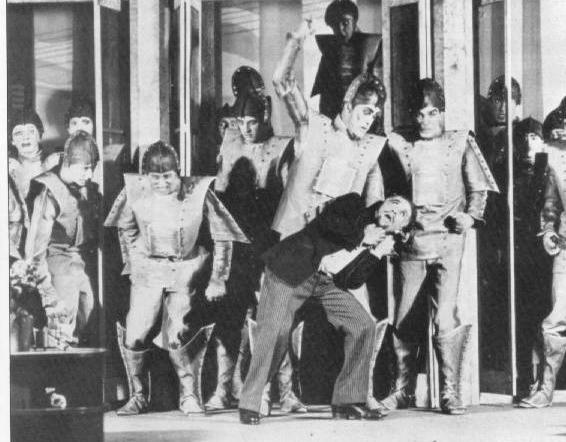
\includegraphics[width=0.4\textwidth]{introduction/rur.jpg}
     \vspace{-15pt}
  \end{center}
  \caption{A `robot' rebellion from Karel Capek's 1920 play, \textit{Rossum's Universal Robots}.}
  \vspace{-5pt}
  \label{fig:into_rur}
\end{wrapfigure}

Autonomous systems, in some form, have been imagined and realized for the bulk of recorded history. In ancient Greek mythology, the god Hephaestus, the `patron of invention and technology' \citep{MayorGodsRobots2019} was said to create talking mechanical hand-maidens, while early Hindu and Buddhist texts tell of \textit{yantakara} that lived in Greece and created machines that helped in trade and farming. The secret methods of the \textit{yantakara} (the early `roboticists') were closely guarded, and mechanical assassins were said to pursue and kill any person who revealed their techniques\footnote{Please be careful distributing this thesis.} \citep{MayorGodsRobots2019}. 
%https://scroll.in/article/916490/in-an-ancient-indian-legend-robots-guarded-buddhas-relics
%Cite 


Since the industrial revolution, the idea of an autonomous machine--one that requires no, or very minimal, human intervention or oversight to operate--has been imagined in different ways. Depending on one's perspective, autonomous machines have perennially promised to either usher in a utopia of freedom, or threatened to bring about an age of job loss and social upheaval that worsens socioeconomic divisions. Much like the Luddites of the 19th century, the social critics of the 21st century have continued the dialectic to understand the social ramifications of modern \textit{yantakara} and their newly-created autonomous hand-maidens.

These controversial origins are embedded even within the modern name of for the academic field, \textit{robotics}. The word \textit{robot} comes from the title of a science fiction play, R.U.R.: Rossum's Universal Robots, written by the Czech playwright Karel Capek in 1920 (see \Cref{fig:into_rur}). In naming the play, the word \textit{robot} was derived from the Slavic term for slave, \textit{rab}, and its Czech derivative for serf labour, \textit{rabota}, while the name \textit{Rossum} was inspired by the Czech word for reason, or intellect. Indeed, the concept of enslaved or embodied  intelligence is at the heart of modern definitions of the discipline of robotics \citep{Redfield2019-pi}. Much of the popular culture surrounding robots (e.g., Shelley's \textit{Frankenstein}, Asimov's \textit{I, Robot}, Kubrick's and Clarke's \textit{2001: A Space Odyssey}) also paints a complicated picture of humanity's relationship with such enslaved machines. In this dissertation, we focus on improving a specific part of a modern \textit{mobile} autonomy pipeline, while minimizing the use of term \textit{robot} to avoid maelstrom of philosophical and ethical problems that it connotes. We hope this work aids the march of technological progress towards a future which finds some Hegelian synthesis of autonomy and humanity---a future in which human-in-the-loop autonomous systems augment and improve the lot of many people while still negotiating and constantly considering the social costs that come with technological innovation.

\section{Mobile Autonomy and State Estimation}
While the looms and railroads of the industrial revolution were spurred by the discovery of steam engines and electricity, modern \textit{mobile} autonomy was largely born out of the technological arms race of the cold war and the constraints and challenges associated with long-distance flight and extraterrestrial travel (see \cite{Grewal2010-ts} for a history of one of the seminal algorithms in mobile autonomy, the Kalman filter). Indeed, much of the work on modern perception algorithms has its origins in the automated compilation of cold-war-era reconnaissance imagery and the design of extraterrestrial rovers like the Mars Exploration Rovers, \textit{Spirit} and \textit{Opportunity} \citep{Scaramuzza2011-qr}. Similarly, much of the planning and control algorithms originate in American and Soviet defence-funded research \citep{Nilsson1984-oc,Thrun2006-hb}.

%https://mars.nasa.gov/resources/22342/opportunity-legacy-pan-true-color/
\begin{figure}
  \begin{center}
  	\vspace{-10pt}
    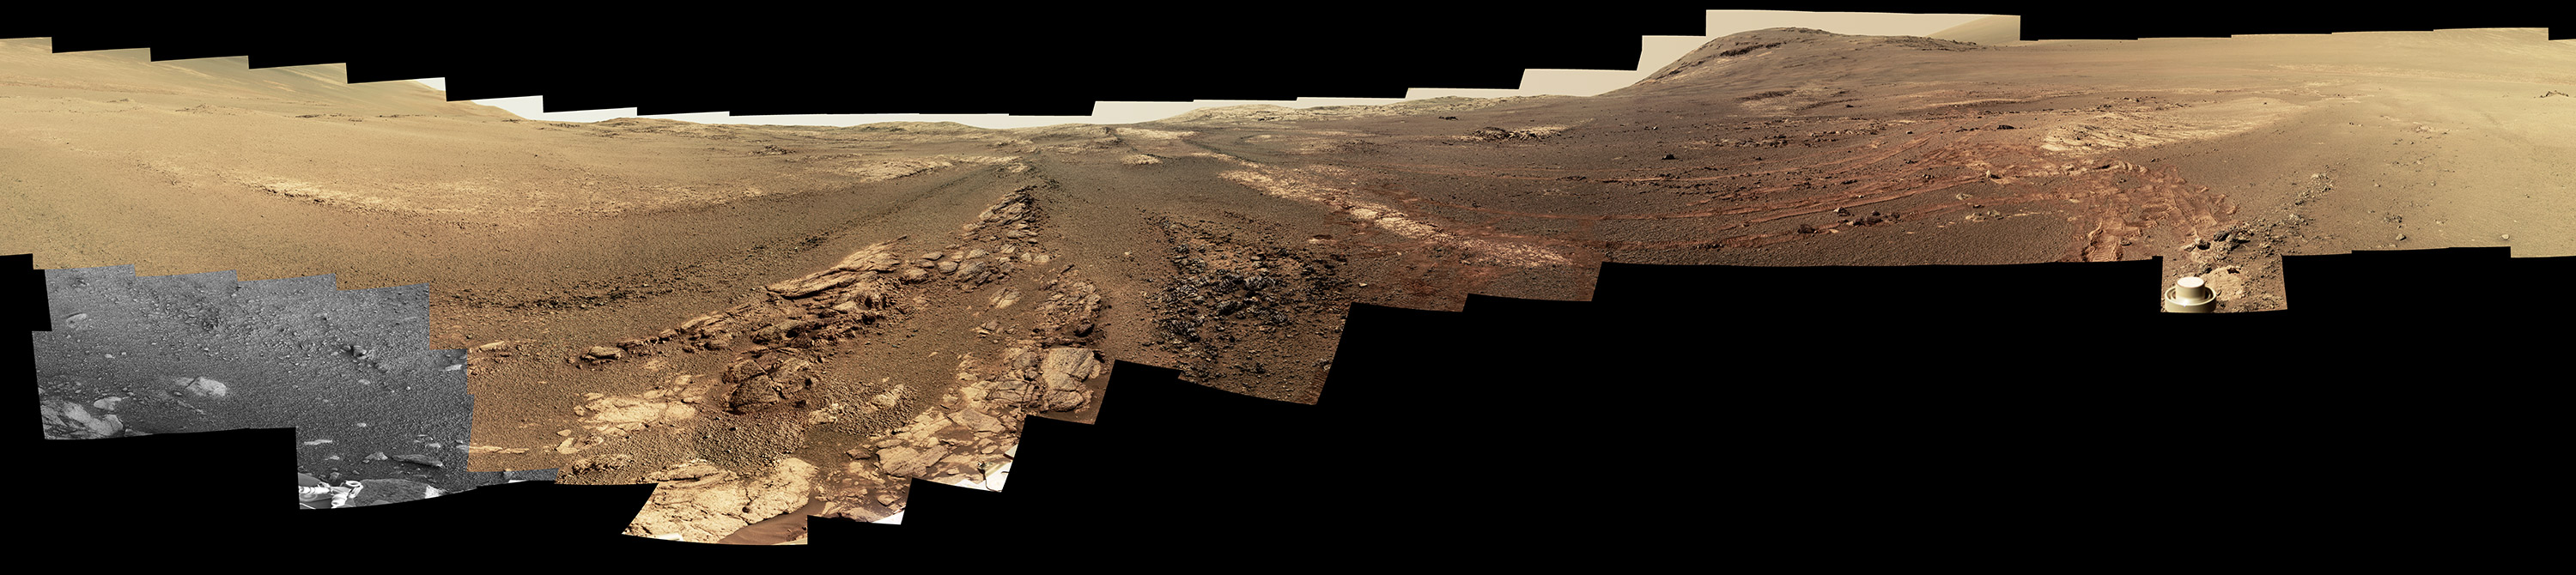
\includegraphics[width=0.95\textwidth]{introduction/pancam-panorama-opportunity}
     \vspace{-15pt}
  \end{center}
  \caption{The last 360 degree panorama taken by the PanCam apparatus of the Mars Exploration Rover, \textit{Opportunity}, at its final resting place on Mars, the western rim of the Endeavour Crater. Contact with \textit{Opportunity} was lost shortly after this was captured, due to a severe dust storm (credit: NASA/JPL-Caltech/Cornell/ASU).}
  \vspace{-5pt}
  \label{fig:into_rur}
\end{figure}


Once confined to carefully-controlled factory floors, autonomous mobile platforms have now began to show great promise in improving the safety of human transport, reducing the burden of repetitive, arduous jobs, and more efficiently leveraging limited resources for environmental monitoring. This newly-realized potential can be attributed to several factors: improvements in the cost and efficiency of computing devices (in terms energy efficiency, processing power, and overall size), the availability of relatively cheap, compact, high-quality sensors and rapid prototyping tools, and the development of open-source hardware, software platforms and datasets (e.g., the Robot Operating System, the KITTI Self-Driving Car dataset \citep{Geiger2013-ky}). 

\begin{figure}
     \centering
     \begin{subfigure}[b]{0.3\textwidth}
         \centering
\def\firstcircle{(0,0) circle (2cm)}
\def\secondcircle{(60:2.75cm) circle (2cm)}
\def\thirdcircle{(0:2.75cm) circle (2cm)}
\scalebox{0.75}{
\begin{tikzpicture}
    \begin{scope}[shift={(3cm,-5cm)}, fill]
        \fill[green!80,opacity=0.5] \firstcircle;
        \fill[blue,opacity=0.5] \secondcircle;
        \fill[black,opacity=0.5] \thirdcircle;
        \draw \firstcircle node [yshift=-1ex,xshift=-2.5ex,align=center] {C. Human\\Interaction};
        \draw \secondcircle node [above,color=white] {A. Software};
        \draw \thirdcircle node [yshift=-1ex,xshift=3ex,color=white] {B. Hardware};
    \end{scope}
\end{tikzpicture}         
}
\caption{Research strands in mobile autonomy.}
 \label{fig:intro_autonomy_venn}
     \end{subfigure}
     \hfill
     \begin{subfigure}[b]{0.3\textwidth}
         \centering
\def\firstcircle{(0,0) circle (2cm)}
\def\secondcircle{(60:2.75cm) circle (2cm)}
\def\thirdcircle{(0:2.75cm) circle (2cm)}
\scalebox{0.75}{
\begin{tikzpicture}
    \begin{scope}[shift={(3cm,-5cm)}, fill]
        \fill[blue,opacity=0.5] \firstcircle;
        \fill[blue!20,opacity=0.5] \secondcircle;
        \fill[blue!60,opacity=0.5] \thirdcircle;
        \draw \firstcircle node [align=center,yshift=-1ex,xshift=-2.5ex,color=white] {A.III.\\Control};
        \draw \secondcircle node [above,align=center,color=black] {A.I.\\Perception};
        \draw \thirdcircle node [align=center,yshift=-1ex,xshift=2.5ex] {A.II.\\ Planning};
    \end{scope}
\end{tikzpicture} 
}        \caption{The components of software research.}
         \label{fig:intro_software_venn}
 \end{subfigure}
 \hfill
      \begin{subfigure}[b]{0.3\textwidth}
         \centering
\def\firstcircle{(0,0) circle (2cm)}
\def\secondcircle{(60:2.75cm) circle (2cm)}
\def\thirdcircle{(0:2.75cm) circle (2cm)}
\scalebox{0.75}{
\begin{tikzpicture}
    \begin{scope}[shift={(3cm,-5cm)}, fill]
        \fill[blue!20,opacity=0.5] \firstcircle;
        \fill[blue!10,opacity=0.5] \secondcircle;
        \fill[blue!5,opacity=0.5] \thirdcircle;
        \draw \firstcircle node [align=center,yshift=-1ex,xshift=-2.5ex] {A.I.3\\Object\\Detection\\ \& Tracking};
        \draw \secondcircle node [above,align=center] {A.I.1.\\Localization};
        \draw \thirdcircle node [align=center,yshift=-1ex,xshift=2.5ex] {A.I.2.\\Mapping};
        \draw[->] (1.2,0.8) -- (3.7,3) node[right,align=left] {State\\Estimation};
    \end{scope}
\end{tikzpicture} 
}        \caption{The components of perception.}
         \label{fig:intro_perception_venn}
 \end{subfigure}
        \caption{Venn diagrams of modern mobile autonomy.}
        \label{fig:intro_three_venn}
\end{figure}

 
 Despite decades of research, mobile autonomy as a field still has nebulous demarcations between subfields. We have attempted to provide a general overview of the field through a series of Venn diagrams in \Cref{fig:intro_three_venn}.  At the highest level, the field can be roughly divided into those researchers who study and develop software, those who study and develop hardware, and those who study and analyze the interaction between autonomous systems (composed of both software and hardware) and humans (\Cref{fig:intro_autonomy_venn}). There is, of course, a plethora of overlap between all three of these rough categories. Within the software realm, there has historically been a distinction between those who study algorithms that deal with the perception of the interoceptive and exteroceptive data, those who study how to use that data to plan action, and those who study how to use those plans to control a system to execute that action (\Cref{fig:intro_software_venn}). 
 
 %Add some discussion about computer science vs. robotics research
 
 Within perception, which is the focus of this dissertation, there are three general directions of research: localization, mapping, and object detection and tracking. Localization and mapping can refer to self-localization, or egomotion estimation, which deals with the problem of estimating the pose of a moving platform through an unknown world, SLAM, simultaneous localization and mapping, which deals with the former problem and mapping simultaneously or finally, it can refer to localization within a known map given some hitherto unseen observation of that environment. The field of object detection and tracking (whether that be static objects like stop signs, or moving objects like humans, animals or vehicles) uses much of the same underlying mathematics as the former two, but has historically been a separate strand of research. Broadly, the overlap of all three of these pursuits within the field of autonomy and robotics is referred to as \textit{state estimation} \citep{Barfoot2017-ri}. To provide context for the central concept of this thesis, a \textit{pseudo-sensor}, we will first outline a traditional approach to state estimation.
 %https://tex.stackexchange.com/questions/9681/how-to-draw-venn-diagrams-especially-complements-in-latex 


\section{The \textit{State} of State Estimation}

\begin{figure}
\begin{center}
		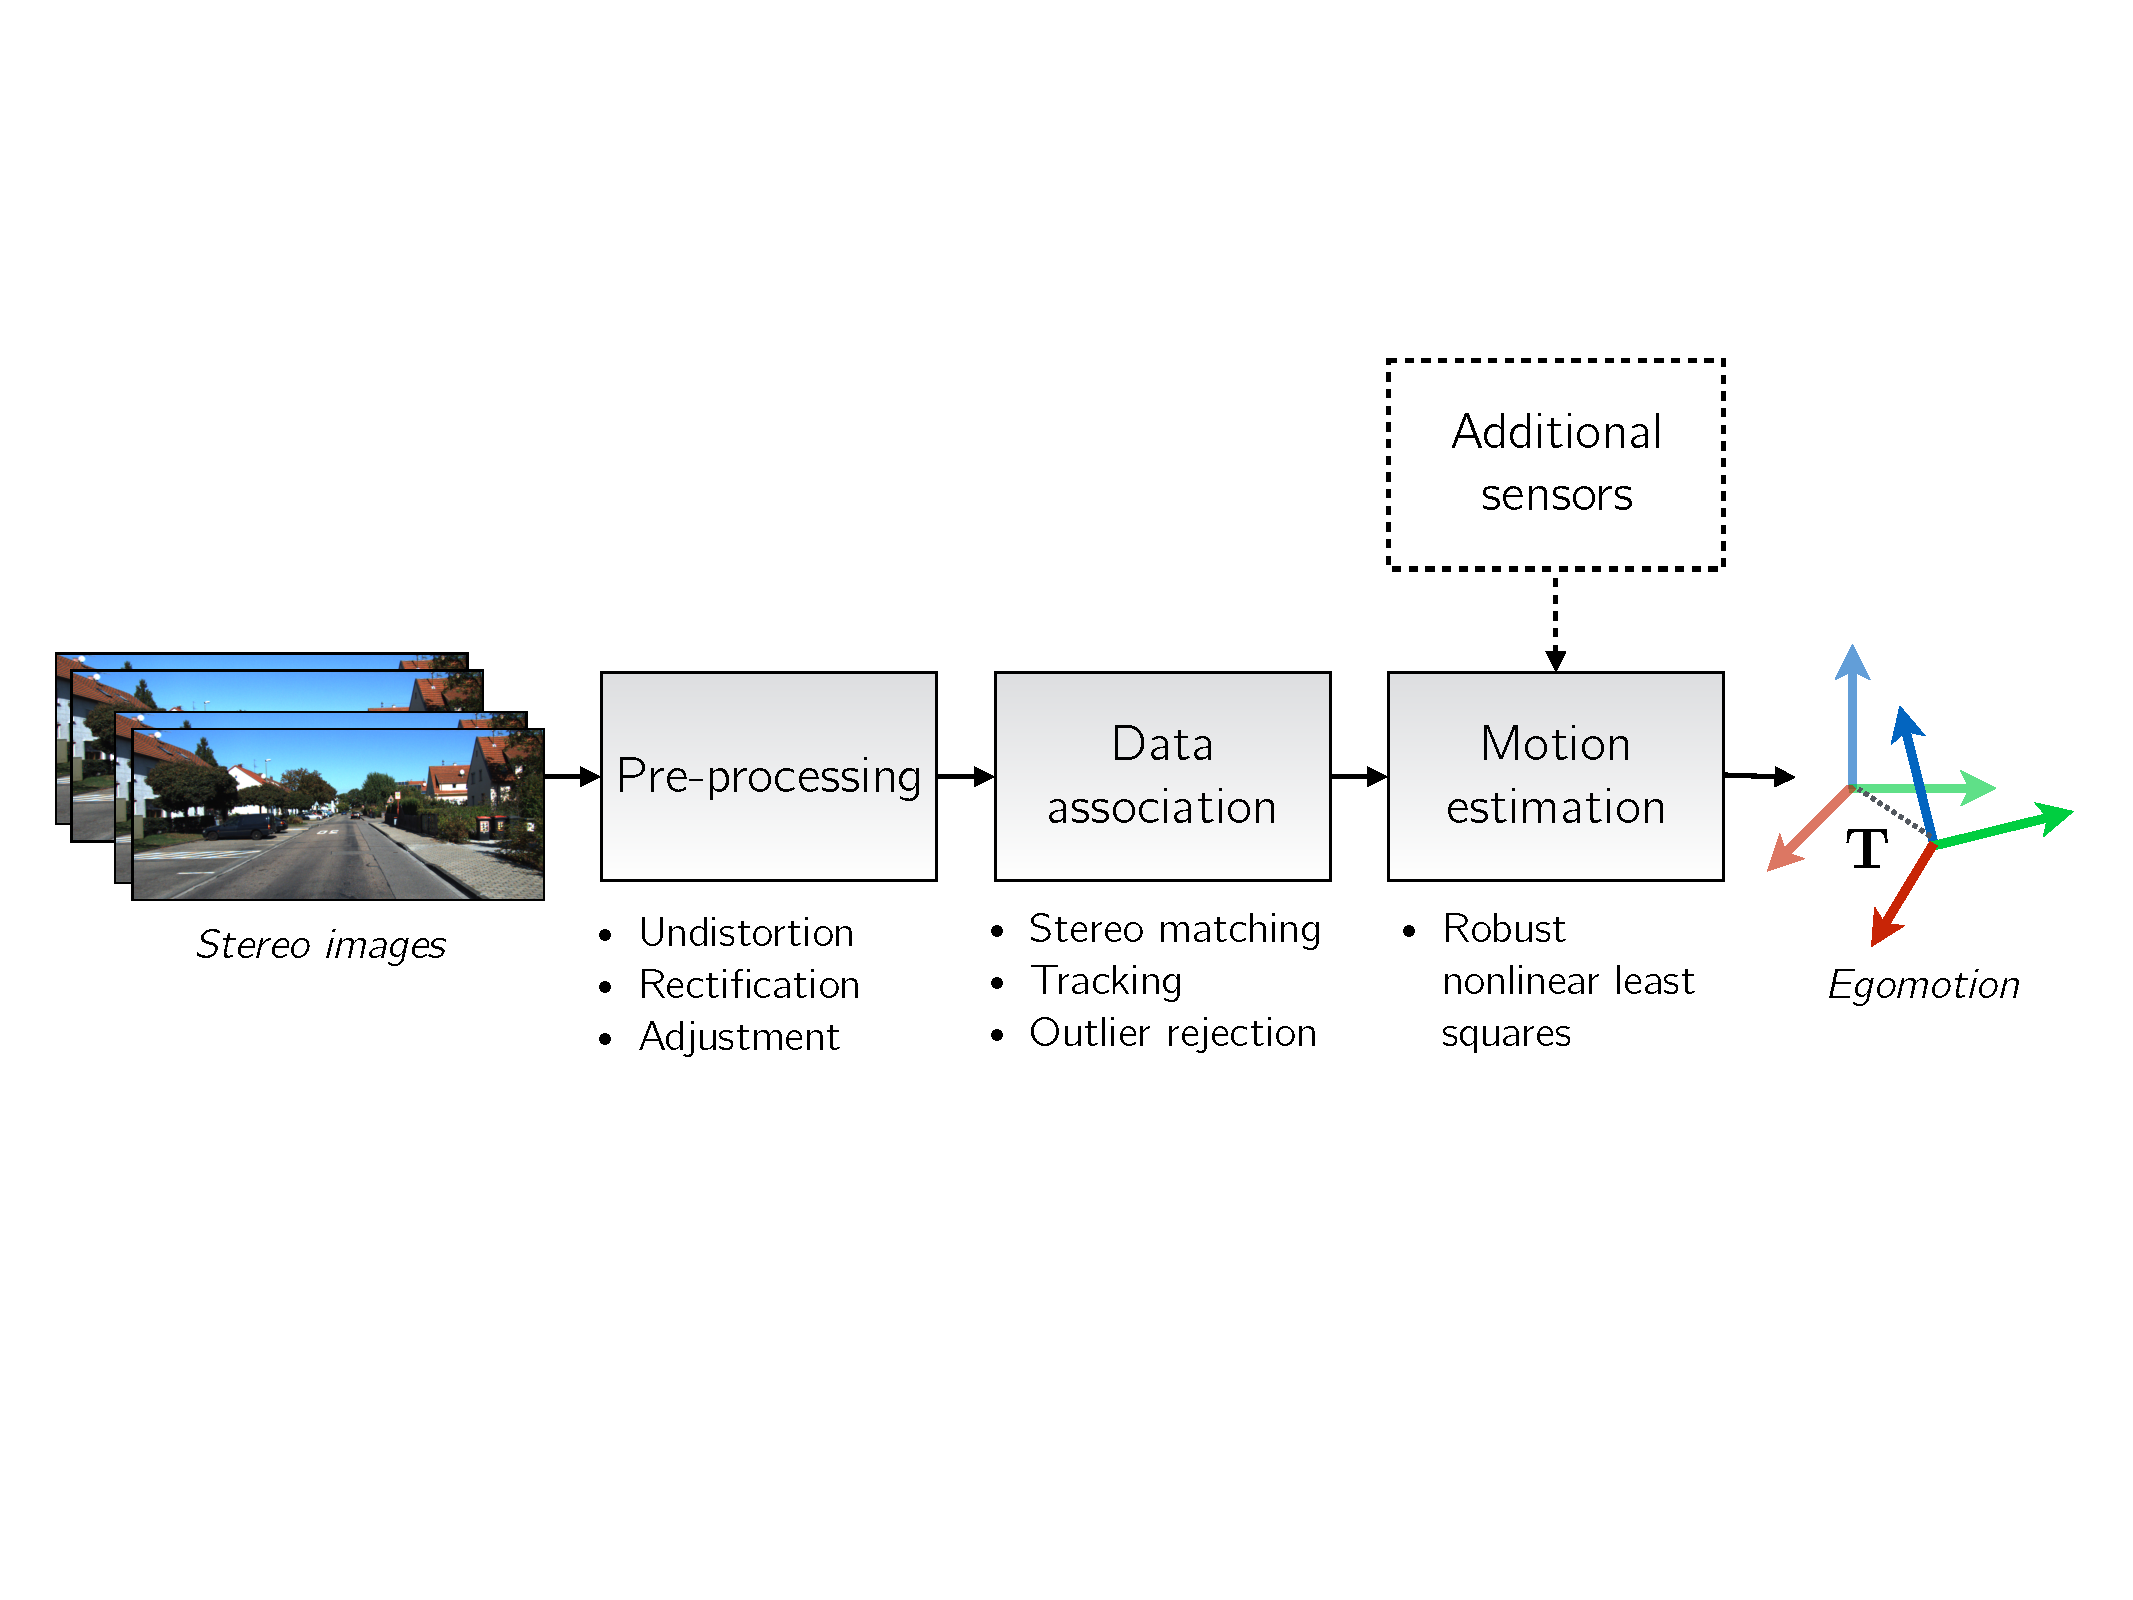
\includegraphics[width=0.98\textwidth]{introduction/vo_pipeline.pdf}
		\caption{A `classical' visual odometry pipeline consists of several distinct components that have interpretable inputs and outputs.}
  	\label{fig:intro_vo_pipeline}
\end{center}
\end{figure}


Central to \textit{classical} state estimation algorithms (which, in this context, refers to the bulk of state estimation research published during what \cite{Cadena2016-ds} call the \textit{classical} and \textit{algorithmic-analysis} ages of SLAM research between 1986 and 2015) is the idea of a pipeline. A pipeline consists several distinguishable blocks that have interpretable inputs and outputs.  By carefully processing information contained within sensor data, pipelines facilitate the construction of complex state estimation architectures that can fuse observations from sensors of varied modality to create rich models of the external world and infer the state of a mobile platform within it. This dissertation focuses on egomotion estimation: the problem of accurately and consistently estimating the relative pose of a moving platform. For this task, a variety of different sensors may be useful (e.g., lidar, stereo cameras, or inertial measurement units), and each may allow for various components of a state estimation pipeline. For cameras, egomotion estimation is typically referred to as \textit{visual odometry} or VO for short. In this thesis, we will largely deal with the improvement of a `classical' VO pipeline-- we illustrate its major components in \Cref{fig:intro_vo_pipeline}. 




Modern VO pipelines (e.g., \cite{Leutenegger2015-fk, Cvisic2015-mt, Tsotsos2015}) have achieved impressive localization accuracy on trajectories spanning several kilometres by carefully extracting and tracking sparse visual features (using \textit{hand-crafted} algorithms) across consecutive images. Simultaneously, significant effort has gone to developing localization pipelines that eschew sparse features in favour of \textit{dense} visual data \citep{Alcantarilla2016-kv, forster2014svo}, typically relying on loss functions that use direct pixel intensities. 

In the last five years, a significant part of the visual state estimation literature has also focused on the idea of replacing classical pipelines with parametric modelling through deep convolutional neural networks (CNNs) and data-driven training. Although initially developed for image classification  \citep{LeCun2015-qf}, CNN-based measurement models have been applied to numerous problems in geometric state estimation (e.g., homography estimation \citep{DeTone2016-ue}, single image depth reconstruction \citep{Garg2016-ip},  camera re-localization \citep{Kendall2016-zf}, place recognition \citep{Sunderhauf2015-is}). A number of recent CNN-based approaches have also tackled the problem of egomotion estimation, often purporting to obviate the need for classical visual localization pipelines by learning pose changes \textit{end-to-end}, directly from image data (e.g., \cite{Melekhov2017-dl}, \cite{Handa2016-hm}, \cite{Oliveira2017-lt}).

Despite this surge of excitement, significant debate has emerged within the robotics and computer vision communities regarding the extent to which deep models should replace existing geometric state estimation algorithms. Owing to their representational power, deep models may move the onerous task of selecting `good' (i.e., robust to environmental vagaries and sensor motion) visual features from the roboticist to the learned model. By design, deep models also provide a straight-forward formulation for using \textit{dense} data while being flexible in their loss function, and taking full advantage of modern computing architecture to minimize run-time. Despite these potential benefits, current deep regression techniques for state estimation often generalize poorly to new environments, come with few analytical guarantees, and provide only point estimates of latent parameters. Indeed, the most accurate visual egomotion pipelines\footnote{Cite KITTI leaderboard} largely those based on carefully selected sparse features. Furthermore, there is recent empirical evidence \citep{Zhou2019-se} that suggests that designing a pipeline with interpretable components (e.g., optical flow, scene segmentation) is crucial to generalization on various visual tasks. We summarize the benefits and detriments to using deep models (as opposed to classical pipelines) in \Cref{tab:intro_classical_vs_deep}. 

\begin{figure}
\begin{center}
		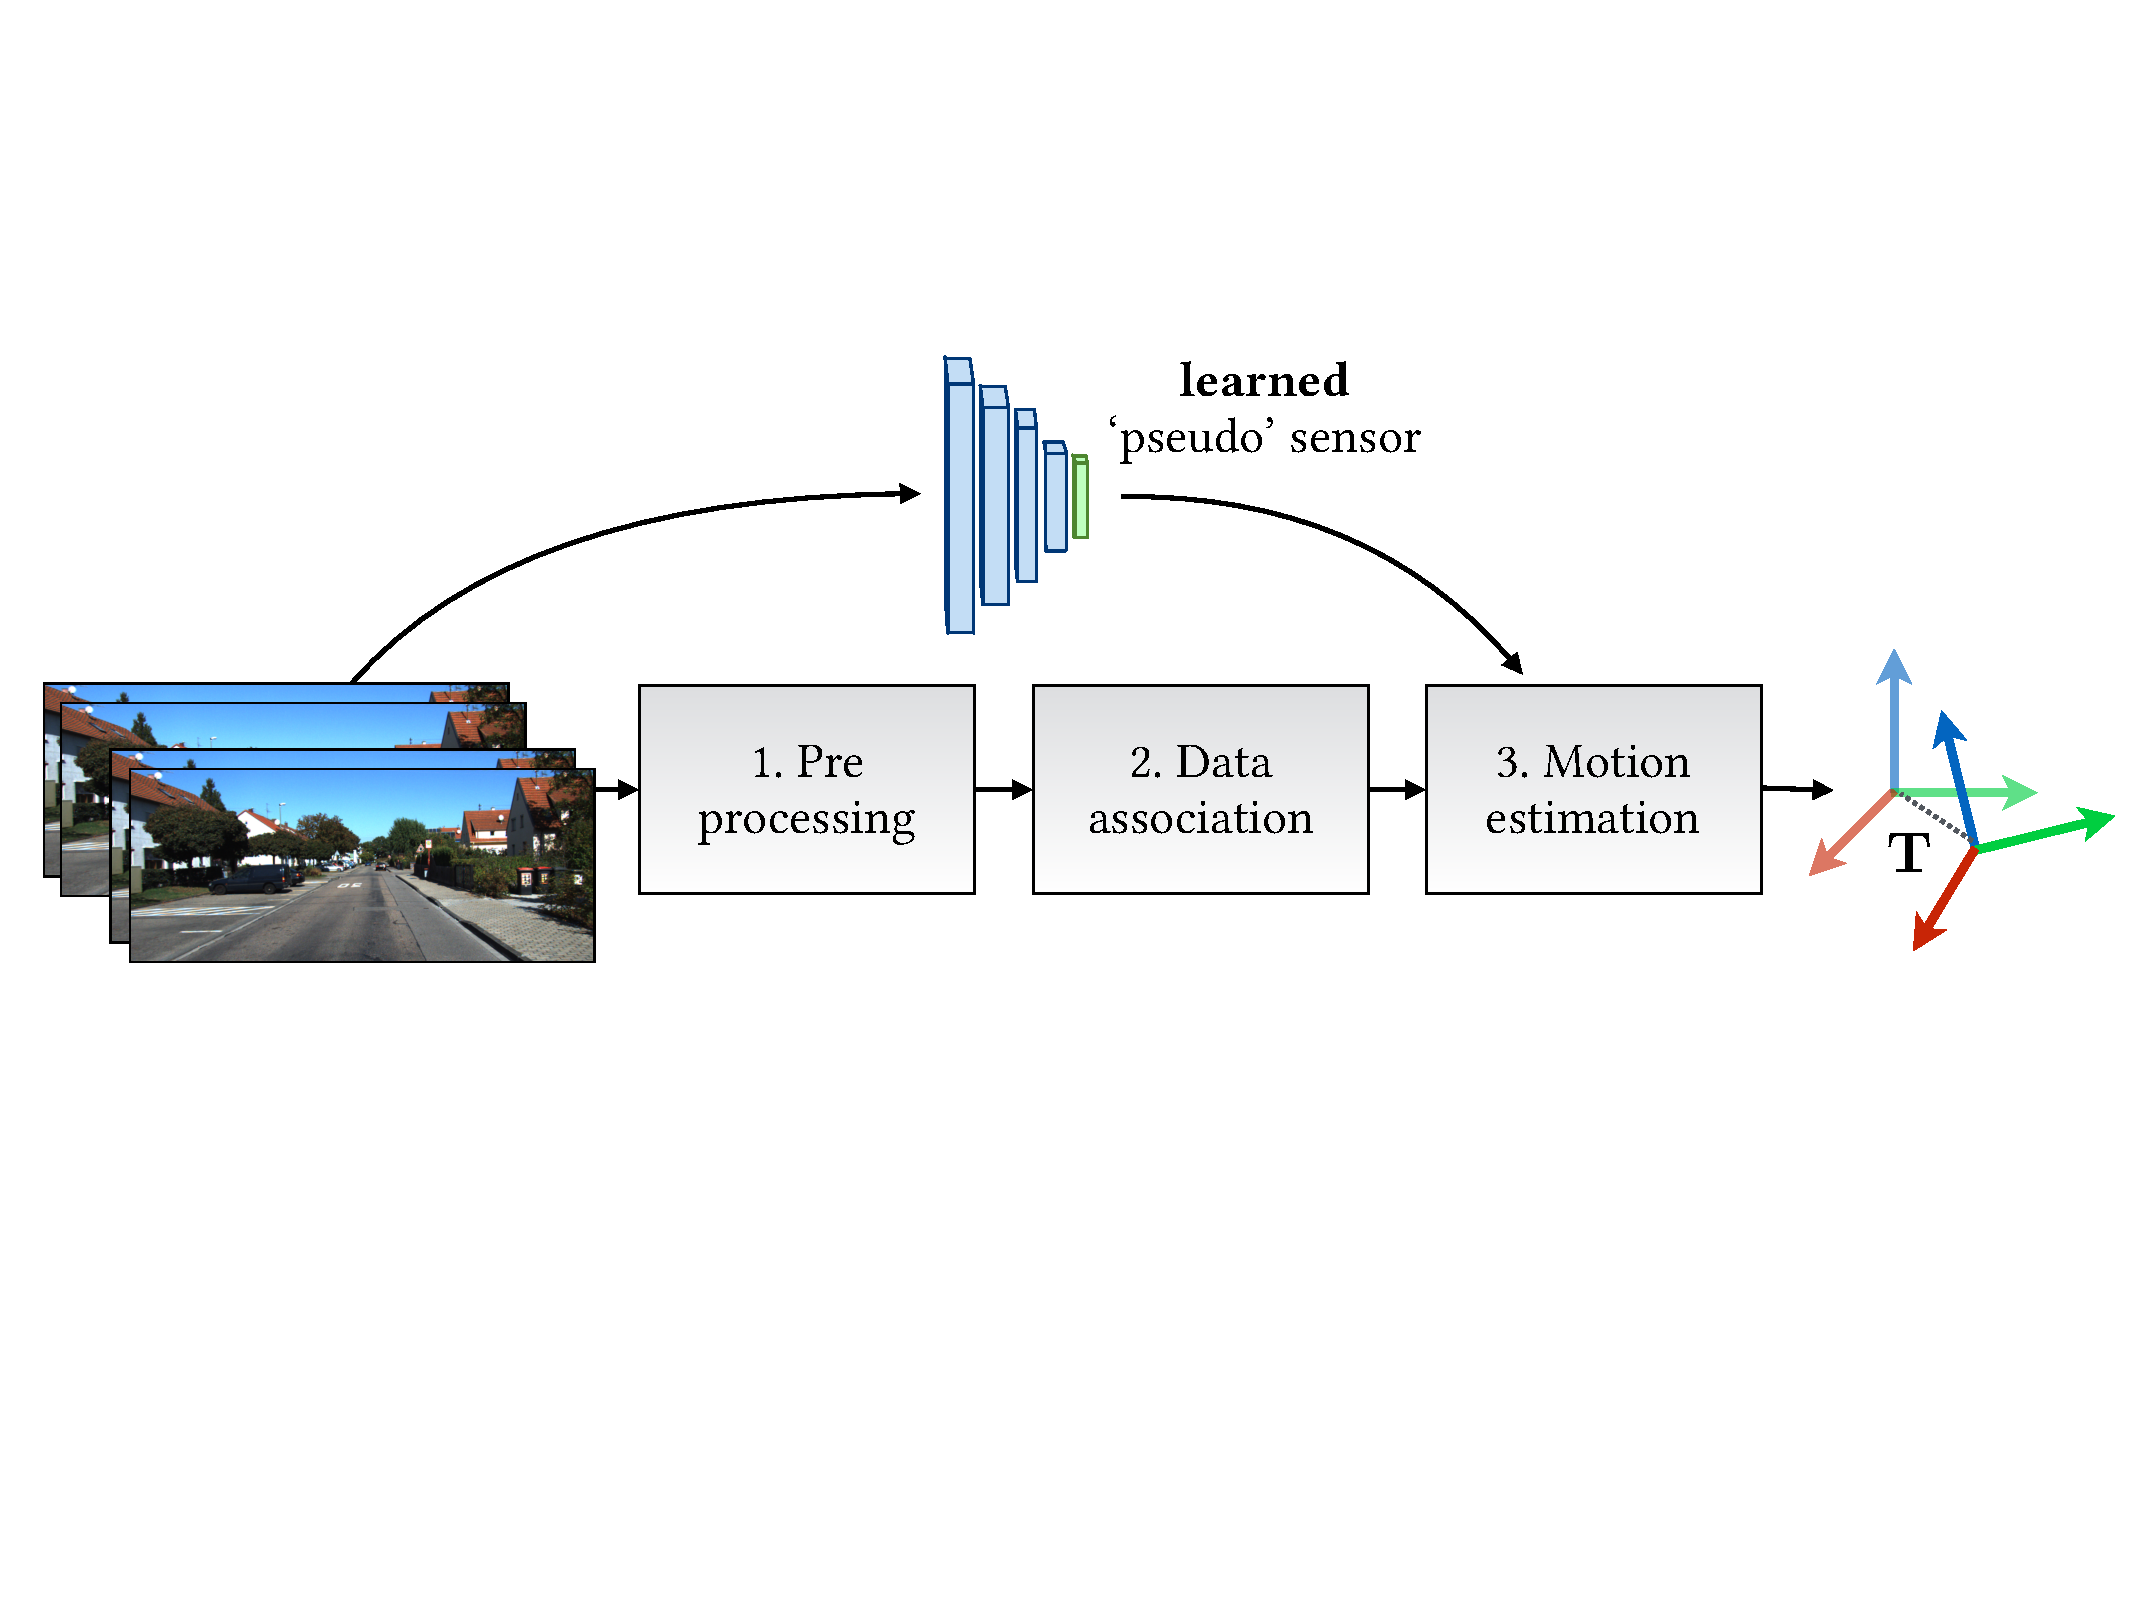
\includegraphics[width=0.98\textwidth]{introduction/pseudo_sensor.pdf}
		\caption{A learned \textit{pseudo-sensor} extracts latent information from the same data stream.}
  	\label{fig:intro_pseudo_sensor}
\end{center}
\end{figure}


\begin{table}[h!]
	\caption{A comaprison of pipelines and end-to-end deep models for visual egomotion estimation.}
	\begin{threeparttable}
	\begin{tabular}{m{0.18\textwidth}m{0.38\textwidth}m{0.38\textwidth}}
		\toprule
		& \textbf{Classical Pipelines} & \textbf{Deep Models} \\ \midrule  
		\textit{Maturity} & Decades of literature \& domain knowledge & Nascent with few uses in mobile autonomy \\
		& & \\
		\textit{Interpretability} & Good, each component has interpretable input and output & Poor, often with no interpretable intermediate outputs \\
		& & \\
		\textit{Uncertainty} & Foundational to \textit{probabilistic robotics} & Few nascent methods (Monte-carlo Dropout \citep{Gal2016-ny}, Bootstrap \citep{Osband2016})  \\
		& & \\
		\textit{Robustness} & Empirically generalizable \citep{Zhou2019-se} & Highly dependant on training data\\
		& & \\
		\textit{Flexibility} & Limited by ingenuity of designer & Limited by training data \\
		\bottomrule
	\end{tabular}
\end{threeparttable}
\label{tab:intro_classical_vs_deep}
\end{table}

\section{The Learned Pseudo-Sensor}

As state estimation enters the robust-perception age \citep{Cadena2016-ds}, algorithms that work in limited contexts will need to be adapted and augmented to ensure they can operate over longer time-periods, and through sundry environments. Towards this end, we introduce the paradigm of the \textit{learned pseudo-sensor}. Learned pseudo-sensors allow one to retain the benefits of classical state estimation pipelines while leveraging the representational power of modern data-drive learning techniques. Instead of completely replacing the classical pipeline, herein we present four ways in which machine learning can be used to train a hyper-parametric model (a 'pseudo-sensor') that extracts latent information from an existing visual data stream. By fusing the output of these sensors with the output of the pipeline, we can make the final egomotion estimates more accurate and more robust to difficult-to-model effects (\Cref{fig:intro_pseudo_sensor}). To accomplish this fusion, we rely on two approaches. The first, which is used in Predictive Robust Estimation (PROBE, and its follow up PROBE-GK, \Cref{ch:probe}), treats the pseudo-sensor as a heteroscedastic noise model that can be incorporated into a maximum-likelihood loss. The uncertainty quantification provided by this pseudo-sensor is used to re-weight a loss which can then be minimized through traditional non-linear optimization routines during test-time. The second approach (used by Sun-BCNN, DPC-Net, and HydraNet,  \Cref{ch:sun-bcnn,ch:dpc,ch:hydranet} respectively) produces geometric quantities (probabilistic estimates of an illumination source, $\LieGroupSE{3}$ corrections to existing egomotion estimates, and independent probabilistic rotation estimates, respectively), that can be fused with the original pipeline through a factor graph optimization routine.

%\section{Outstanding Issues in the Field}

%\subsection{The limits of homoscedastic noise models}
%
%Although several state-of-the-art state estimation pipelines  \citep{Leutenegger2015-fk, Cvisic2015-mt} leave observation uncertainty associated with sensor measurements as a static tuning parameter, recent work \citep{Vega-Brown2014-sb, Hu2015-uw} suggests that using a stationary, homoscedastic noise in observation models can often reduce the consistency and accuracy of state estimates. This is especially true for complex, inferred measurement models. In foot-mounted navigation, the inferred zero velocity detector may be more or less informative depending on the exact type of motion and individual gait. In visual data, inferred visual observations can be degraded not only due to sensor imperfections (e.g. poor intrinsic calibration, digitization effects, motion blur), but also as a result of the observed environment (e.g. self-similar scenes, specular surfaces, textureless environments). Indeed, robust costs \cite{Alcantarilla2016-kv, MacTavish2015-wt, Agarwal2013-jq} and whiteness tests \citep{Tsotsos2015} have commonly been used to alleviate the problem of poor noise modelling, but more work is required to better learn uncertainty in complex measurement models.
%
%
%\subsection{Deep, learned models with no uncertainty estimates}
%
%Although the paradigm of deep neural networks has resulted in several significant achievements in the fields of computer vision \citep{LeCun2015-qf}, these types of models have largely focused on point estimates (in either regression or classification) without any principled uncertainty estimates. Recently, the regularization techniques of dropout and dropconnect in Convolutional Neural Networks have been linked with approximate variational inference in homoscedastic Gaussian Processes \citep{Gal2015-bf, Kendall2016-zf, McClure2016-ai}, and the statistical technique of \textit{bootstrapping} has been applied to Deep Q Networks \citep{Osband2016-jg} to infer uncertainty, but both techniques are in their infancy. Recent work \citep{Osband_undated-wl} has also suggested that the former technique of dropout-based `uncertainty' is actually a measure of \textit{risk} (i.e., stochasticity in the measurements) and not \textit{uncertainty} over state parameters. Further, the same work showed that even this risk quantification can be arbitrarily bad given a fixed dropout parameter (which is typically the case).
%
%\subsection{Integration of deep models into state estimation pipelines}
%
% To integrate the power of deep networks into state estimation algorithms, the recent literature differs in how to proceed. While some attempt to parametrize geometric transformations in their unconstrained state, and then learn the resulting state within a deep network regression optimization \citep{Costante2016-hb, Kendall2015-kh}, others integrate deep networks within outer estimation loops \citep{Haarnoja2016-ph}. Yet other work has used the neural network as an error correcting mechanism on top on an existing kinematic or dynamic model \citep{Punjani2015-pj}. This integration is made more difficult by the lack of uncertainty estimates associated with many learned measurement models in the computer vision and machine learning literature.
% 
 
\section{Original Contributions}

\begin{figure}[h!]
\begin{center}
		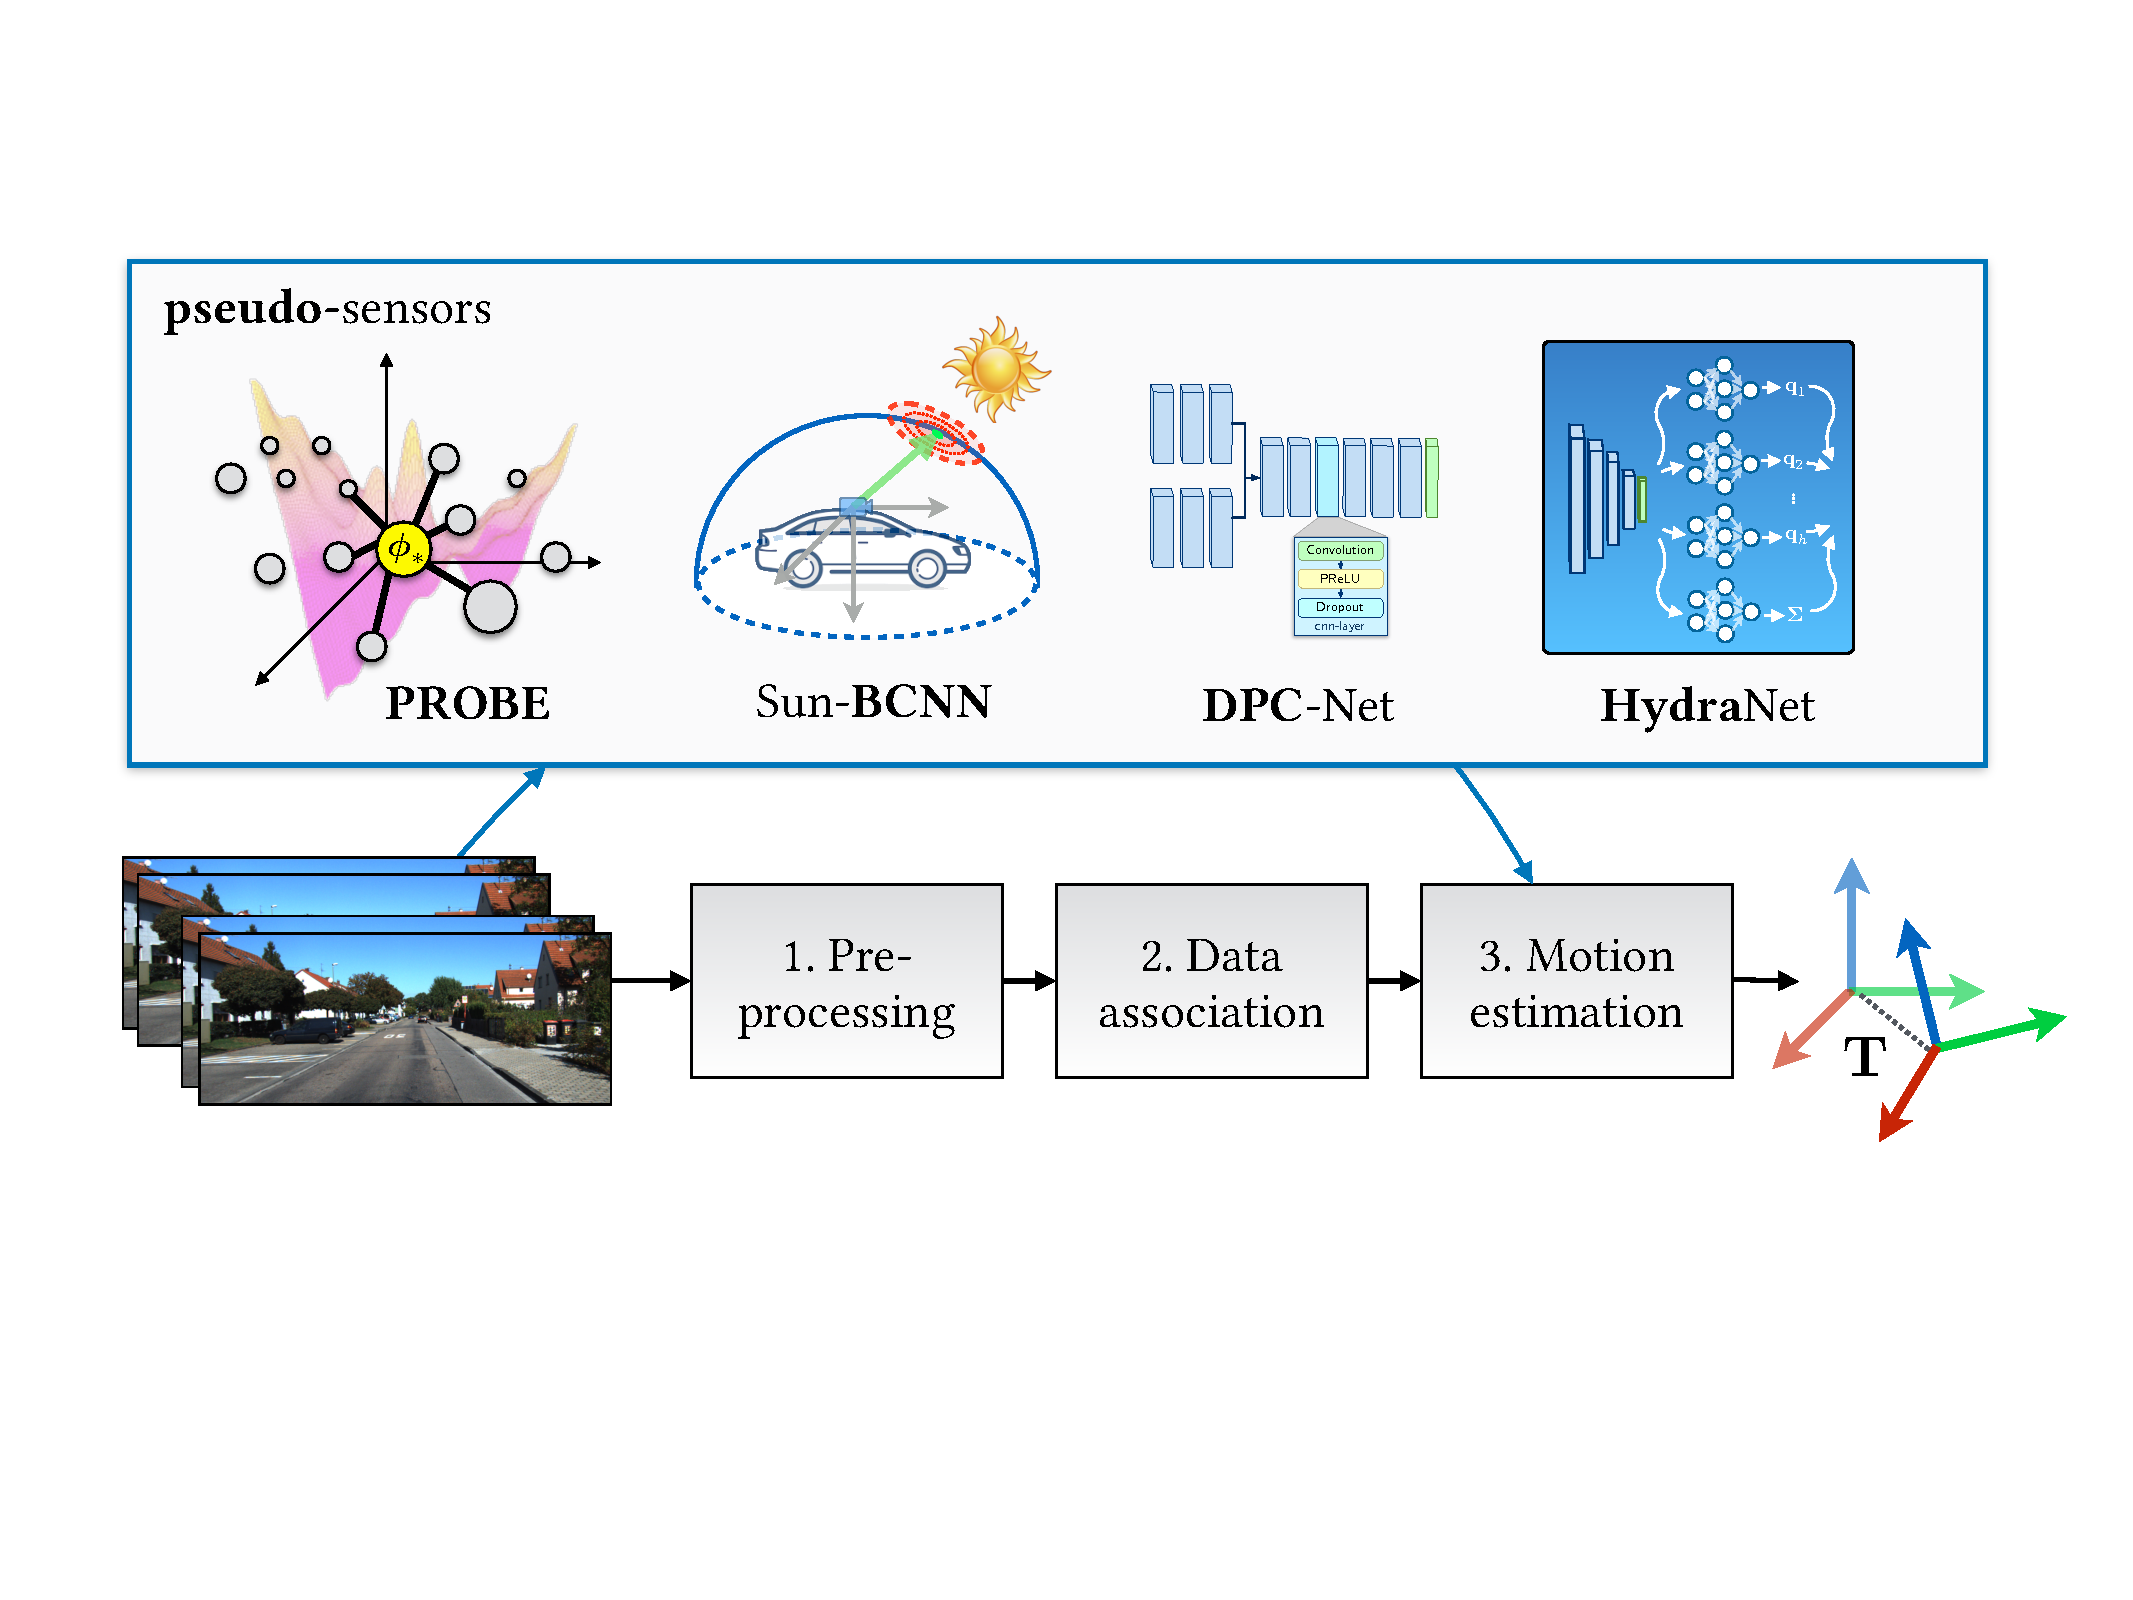
\includegraphics[width=0.98\textwidth]{introduction/all_pseudo_sensors.pdf}
		\caption{This dissertation details four examples of \textit{pseudo-sensors} that improve 'classical` egomotion estimation through data-driven learning.}
  	\label{fig:intro_pseudo_sensors}
\end{center}
\end{figure}


This dissertation consists of several published contributions under the umbrella of a \textit{learned pseudo-sensor} that improves a canonical visual egomotion pipeline. Before detailing each pseudo-sensor, we present some mathematical foundations (\Cref{ch:math}) and a common baseline for an indirect stereo visual odometry pipeline (\Cref{ch:vo}) which all four methods build upon. In total, there are two journal papers, and five conference papers associated with our work. Below, we briefly summarize each of the pseudo-sensors and list the publications that are associated with each.
\begin{enumerate}
\item \textbf{Predictive Robust Estimation (PROBE)},  \\
Predictive Robust Estimation (\Cref{ch:probe}) uses k-NN regression (original PROBE) or Generalized Kernels \citep{Vega-Brown2014-sb} (PROBE-GK) to train a predictive model for heteroscedastic measurement covariance of stereo reprojection errors to improve the accuracy and consistency of an indirect stereo visual odometry pipeline. It is associated with three publications:
\begin{itemize}
\item \bibentry{2015_Peretroukhin_PROBE}
\item \bibentry{2015_Peretroukhin_Get}
\item \bibentry{Peretroukhin2016-om}
\end{itemize}

\item \textbf{Virtual Sun Sensor using a Bayesian Convolutional Neural Network} \\ 
Sun-BCNN (\Cref{ch:sun-bcnn}) is a technique to infer a probabilistic estimate of the direction of the sun from a single RGB image using a Bayesian Convolutional Neural Networks (BCNN). The method works much like dedicated sun sensors \citep{Lambert2012-sn}, but requires no additional hardware, and can provide mean and covariance estimates that can be readily incorporated into existing visual odometry frameworks.  It is associated with three publications listed below. Initial exploratory work was published at ISER 2016, and the BCNN improvement was presented at ICRA 2017. An additional journal paper summarizing the work of the prior two papers, adding data from the Canadian High Arctic and Oxford, and investigating the effect of cloud cover and transfer learning was published in the International Journal of Robotics' Research, Special Issue on Experimental Robotics at the end of 2017. 
\begin{itemize}
\item \bibentry{2017_Clement_Improving}
\item \bibentry{2017_Peretroukhin_Reducing}
\item \bibentry{2018_Peretroukhin_Inferring}
\end{itemize}

\item \textbf{Deep Pose Corrections (DPC-Net)} \\
Deep Pose Correction (\Cref{ch:dpc}) is an approach to improving egomotion estimates through pose corrections learned through deep regression. DPC takes as its starting point an efficient, classical localization algorithm that computes high-rate pose estimates. To it, it adds a Deep Pose Correction Network (DPC-Net) that learns low-rate, `small' \textit{corrections} from training data that are then fused with the original estimates. DPC-Net does not require any modification to an existing localization pipeline, and can learn to correct multi-faceted errors from estimator bias, sensor mis-calibration or environmental effects. It is associated with a journal publication:
\begin{itemize}
\item \bibentry{2018_Peretroukhin_Deep}.
\end{itemize}

\item \textbf{Estimating Rotation through Deep Probabilistic Inference with HydraNet}

Finally, HydraNet (\Cref{ch:hydranet}) is a multi-headed network structure that can regress probabilistic estimates of rotation (elements of the matrix Lie group, $\LieGroupSO{3}$ accounting for both aleatoric and epistemic uncertainty. This uncertainty can then be used to fuse the output of HydraNet with the output of classical egomotion pipelines in a probabilistic factor graph formulation. It is associated with one publication:

\begin{itemize}
\item \bibentry{2019_Peretroukhin_Deep}.
\end{itemize}


\end{enumerate}

%\subsection{Software Contributions}
%
%\begin{itemize}
%\item DPC-Net
%\item SO(3) Learning
%\item \texttt{liegroups}
%\item pyslam 	
%\end{itemize}







\chapter{Mathematical Foundations}
\label{ch:math}
\epigraph{By relieving the brain of all unnecessary work, a good notation sets it free to concentrate on more advanced problems, and, in effect, increases the mental power of the race.}{\textsc{Alfred North Whitehead}}
  \section{Coordinate Frames}

Before we can present the main contributions of this thesis, it will be useful to first outline the notation and mathematical foundations that underly the work. Throughout this thesis, we largely follow the notation of \cite{Barfoot2017-ri} when dealing with three-dimensional rigid-body kinematics. 

\begin{figure}[h!]
\center
\tdplotsetmaincoords{60}{110}
%
\pgfmathsetmacro{\rvec}{1.75}
\pgfmathsetmacro{\thetavec}{45}
\pgfmathsetmacro{\phivec}{60}
%
\begin{tikzpicture}[scale=5,tdplot_main_coords]
\coordinate (O) at (0,0,0) node[anchor=south east]{$\CoordinateFrame{o}$};
\draw[very thick,->, red] (0,0,0) -- (0.7,0,0);
\draw[very thick,->, green] (0,0,0) -- (0,0.7,0);
\draw[very thick,->, blue] (0,0,0) -- (0,0,0.7);
\tdplotsetcoord{V}{\rvec}{\thetavec}{\phivec}
\tdplotsetrotatedcoords{\phivec}{\thetavec}{0} 
\tdplotsetrotatedcoordsorigin{(V)}

\draw [fill, tdplot_rotated_coords] (.3,.3,.3) circle [radius=0.01] node[anchor=north west]{$p$};
\draw[-stealth,tdplot_rotated_coords, black] (O) -- (.31,.31,.31) node[midway,below] {$\VectorArrow{r}^{po}$} ;


\end{tikzpicture}
\caption{A position vector expressed in a coordinate frame.}
\end{figure}

We refer to a three-dimensional position vector, $\VectorArrow{r}^{po}$, as one that originates at the origin of a coordinate reference frame, $\CoordinateFrame{o}$, and terminates at the point $p$. This geometric quantity has the numerical coordinates $\Vector{r}^{po}_o$ when expressed in $\CoordinateFrame{o}$. Often, we will refer to two reference frames such as a world or \textit{inertial} frame,  $\CoordinateFrame{i}$, and a vehicle frame, $\CoordinateFrame{v}$. Rotation matrices or rigid-body transformations that convert coordinates from $\CoordinateFrame{i}$ to $\CoordinateFrame{v}$ will be represented as $\Transform_{vi}$, and $\Rotation_{vi}$\footnote{We use $\Rotation$ and not $\Matrix{R}$ for rotation matrices to avoid confusion with common notation for measurement model covariance.}, respectively. 


\begin{figure}[h!]
\center
\tdplotsetmaincoords{60}{110}
%
\pgfmathsetmacro{\rvec}{1.75}
\pgfmathsetmacro{\thetavec}{45}
\pgfmathsetmacro{\phivec}{60}
%
\begin{tikzpicture}[scale=5,tdplot_main_coords]
\coordinate (O) at (0,0,0) node[anchor=south east]{$\CoordinateFrame{i}$};
\draw[very thick,->, red] (0,0,0) -- (0.7,0,0);
\draw[very thick,->, green] (0,0,0) -- (0,0.7,0);
\draw[very thick,->, blue] (0,0,0) -- (0,0,0.7);
\tdplotsetcoord{V}{\rvec}{\thetavec}{\phivec}
\draw[-stealth] (O) -- (V) node[midway,above] {$\VectorArrow{t}^{vi}$} ;

\tdplotsetrotatedcoords{\phivec}{\thetavec}{0} 
\tdplotsetrotatedcoordsorigin{(V)}


%Coordinate frame with label
\draw[very thick,tdplot_rotated_coords,->, red] (0,0,0) -- (.4,0,0);
\draw[very thick,tdplot_rotated_coords,->, green] (0,0,0) -- (0,.4,0);
\draw[very thick,tdplot_rotated_coords,->, blue] (0,0,0)-- (0,0,.4);
\draw[tdplot_rotated_coords] (0,0,0) node[anchor=south east] {$\CoordinateFrame{v}$};

%Local vector
\draw [fill, tdplot_rotated_coords] (.31,.31,.31) circle [radius=0.01] node[anchor=north west]{$p$};
\draw[-stealth,tdplot_rotated_coords, purple] (0,0,0) -- (.3,.3,.3) node[midway,above] {\footnotesize $\VectorArrow{r}^{pv}$};
\draw[-stealth,tdplot_rotated_coords, black] (O) -- (.3,.3,.3) node[midway,below] {$\VectorArrow{r}^{pi}$} ;

\end{tikzpicture}
\label{fig:math_two_ref_frames}
\caption{Two common references frames used throughout this thesis.}
\end{figure}



\section{Rotations} 

The rotation matrix $\Rotation$ is a member of the matrix Lie group $\LieGroupSO{3}$ (the Special Orthogonal group) and can be defined as a matrix as follows:

\begin{equation}
\LieGroupSO{3} = \{ \Rotation \in \Real{}^{3 \times 3} | ~ \Rotation^T\Rotation = \Matrix{1}, \det{\Rotation} = 1  \}.	
\end{equation}

\subsubsection{Active vs. Passive}
An active (or \textit{alibi}) rotation changes the coordinates of a position directly while implicitly assuming that the reference frame is fixed. A passive (or \textit{alias}) rotation rotates the reference frame. Following \cite{Barfoot2017-ri}, all rotation matrices in this dissertation are passive unless otherwise noted.  

\subsubsection{Exponential and Logarithmic Maps}

Since rotations form a matrix Lie group (we refer the reader to \cite{Sola2018-kg} and \cite{Barfoot2017-ri} for a thorough treatment of Lie groups for state estimation), we can define a surjective exponential map\footnote{We follow \cite{Sola2018-kg} and also define \textit{capitalized} map for notational clarity.} from three axis-angle parameters, $\RotationVector = \phi \RotationAxisVector, ~~ \phi \in \Real{}, \RotationAxisVector \in S^2$, to a rotation matrix, $\Rotation$: 
\begin{align}
\label{eq:so3_exp}
\Rotation = \MatExp{\Vector{\phi}} = \Matexp{\Vector{\phi}} &= \sum_{n=0}^{\infty}  \frac{1}{n!} {(\Vector{\phi}^\wedge)}^n\\
\label{eq:euler_rodriguez}
&= \cos{\phi} \IdentityMatrix + (1 - \cos{\phi}) \RotationAxisVector\RotationAxisVector^T + \sin{\phi} \RotationAxisVector^\wedge,
\end{align}

where the wedge operator $(\cdot)^\wedge$\footnote{This operator is sometimes also expressed as $(\cdot)^\times$ or $[\cdot]_\times$ and is known as the skew-symmetric operator.} is defined as
\begin{equation}
\RotationAxisVector^\wedge = \bbm a_0 \\ a_1 \\ a_2 \ebm^\wedge = \bbm 0 & -a_2 & a_1 \\ a_2 & 0 & -a_0 \\ -a_1 & a_0 & 0 \ebm.	
\end{equation}

\Cref{eq:euler_rodriguez} is known as the Euler-Rodriguez formula and it can also be derived geometrically, starting from Euler's theorem that any rotation can be expressed as an axis of rotation and an angle of rotation about that axis. Although  the map in \Cref{eq:so3_exp} is surjective, we can define an inverse map if we restrict its domain to $0 \leq \phi < \pi$:

\begin{align}
\label{eq:so3_log}
\RotationVector =  \MatLog{\Rotation} = \Matlog{\Rotation} &= \frac{\phi (\Rotation - \Rotation^T)^\vee}{2 \sin{\phi}}, 
\end{align}

where $\phi = \arccos{\frac{\Trace{\Rotation} - 1}{2}}$ and the \textit{vee} operator, $(\cdot)^\vee : \Real{}^{3 \times 3} \rightarrow \Real{}^3$, is defined as the unique inverse of the wedge operator $(\cdot)^\wedge$. Note \Cref{eq:so3_log} is undefined at both $\phi = 0$ and at $\phi = \pi$. In the former case, we can use a small-angle approximation and define

\begin{equation}
	\MatLog{\Rotation} \approx (\Rotation - \IdentityMatrix)^\vee ~~ \textrm{when} ~~ \phi \approx 0. 
\end{equation}

The latter case (when $\phi = \pi$) defines the \textit{cut locus} of the space where $\MatExp{\cdot}$ is not a covering map and both $+\RotationVector$ and $-\RotationVector$ map to the same $\Rotation$. This \textit{cut locus} is related to the idea that any three parameterization of $\LieGroupSO{3}$ will have singularities associated with it.

\subsection{Unit Quaternions}

Another way (and historically, the original way) to represent a general rotation is to use a unit quaternion, $\quat$. A unit quaternion has four parameters, a scalar value $q_\omega$, and a three-dimensional vector component, $\quat_v$:

\begin{equation}
	\quat = \bbm q_\omega \\ \quat_v \ebm \in S^3, ~~ (\Norm{\quat} = 1).
\end{equation}
Unit quaternions also form a Lie group \citep{Sola2018-kg} and and lie on a three-dimensional unit sphere within $\Real{}^4$. This manifold represents a double cover of $\LieGroupSO{3}$ (since both $\quat$ and $-\quat$ represent the same rotation). As with rotation matrices, we can define a surjective map from three parameters to the group itself,

\begin{equation}
\quat = \MatExp{\RotationVector} = \bbm \cos{\phi/2} \\ \RotationAxisVector \sin{\phi/2} \ebm.	
\end{equation}
Similarly, we can also define a logarithmic map as
\begin{align}
\label{eq:math_quat_log}
	\RotationVector =  \MatLog{\quat} = 2 \quat_v \frac{\arctan{(\Norm{\quat_v},  q_\omega})}{\Norm{\quat_v}}.
\end{align}

\noindent To avoid issues with the double cover, we replace $\quat$ with $-\quat$ if $q_\omega$ is negative before evaluating \Cref{eq:math_quat_log}. Also note again that \Cref{eq:math_quat_log} is undefined when $\phi = 0$, but, importantly, we do not face any issues when $\phi = \pi$ due to the half angle. As with rotation matrices, we can use small angle approximations to define:

\begin{equation}
	\MatLog{\quat} \approx \frac{\quat_v}{q_\omega} \left( 1 - \frac{\Norm{\quat_v}^2}{3 q_\omega^2}\right) ~~ \textrm{when} ~~ \phi \approx 0. 
\end{equation}

A fantastic summary of the history of rotation parameterizations, unit quaternions and the story of Hamilton and Rodriguez can be found in \cite{Altmann1989-ru}.



\section{Spatial Transforms}
The rigid body transform $\Transform$ is a also a member of the matrix Lie group, the Special Euclidian group $\LieGroupSE{3}$ and can be defined as a $4 \times 4$ matrix as follows:

\begin{equation}
\LieGroupSE{3} = \{ \Transform = \bbm \Rotation & \Vector{t} \\ \Vector{0}^T & 1 \ebm \in \Real{}^{4 \times 4} | ~  \Rotation \in \LieGroupSO{3},  \Vector{t} \in \Real{}^3  \}.
\end{equation}

As a member of a matrix Lie group, it also admits a surjective exponential map,

\begin{equation}
\Transform = \MatExp{\Vector{\xi}} = \Matexp{\Vector{\xi}} = \sum_{n=0}^{\infty}  \frac{1}{n!} {(\Vector{\xi}^\wedge)}^n	
\end{equation}

where $\TransformVector = \bbm \Vector \rho \\ \Vector \phi \ebm \in \Real{}^6$ and the wedge operator is overloaded (following \cite{Barfoot2017-ri}) as follows:
\begin{equation}
  \Vector \xi^\wedge \triangleq \bbm \Vector \rho \\ \Vector \phi \ebm ^\wedge = \bbm
  \Vector \phi^\wedge & \Vector \rho \\ \Transpose{\Vector{0}} &  0 \ebm.	
\end{equation}

In practice, we can evaluate the exponential map through the Euler-Rodriguez formula (\Cref{eq:euler_rodriguez}) and by computing the left-Jacobian of $\LieGroupSO{3}$,  $\LeftJacobianSO$, 

\begin{equation}
\Transform = \MatExp{\bbm \Vector \rho \\ \Vector \phi \ebm} = \bbm \Rotation(\RotationVector) & \LeftJacobianSO(\RotationVector) \Vector{\rho} \\ \Vector{0}^T & 1 \ebm,
\end{equation}
where
\begin{equation}
\LeftJacobianSO(\RotationVector) = \frac{\sin{\phi}}{\phi} \IdentityMatrix + (1 - \frac{\sin{\phi}}{\phi}) \RotationAxisVector\RotationAxisVector^T + \frac{1 - \cos{\phi}}{\phi} \RotationAxisVector^\wedge.
\end{equation}




\subsection{Applying Transforms}
Applying our notation for coordinate frames (and referring back to \Cref{fig:math_two_ref_frames}), a transform, $\Transform_{vi}$ can be expressed as 
\begin{equation}
\Transform_{vi} = \bbm \Rotation_{vi} & \Vector{t}_v^{iv} \\ \Vector{0}^T & 1 \ebm.
\end{equation}
This allows us to use the homogenous point representation for $\Vector{r}^{pi}_i$ and express the following relation:

\begin{equation}
	\bbm \Vector{r}^{pi}_v \\ 1 \ebm = \underbrace{\bbm \Rotation_{vi} & \Vector{t}_v^{iv} \\ \Vector{0}^T & 1 \ebm}_{\Transform_{vi}} \bbm \Vector{r}^{pi}_i \\ 1 \ebm
\end{equation}
which is numerically equivalent to  

\begin{equation}
 \Vector{r}^{pi}_v =  \Rotation_{vi} \Vector{r}^{pi}_i + \Vector{t}_v^{iv}.  
 \end{equation}

\section{Perturbations}

When solving optimization problems that involve rotations or rigid-body transforms, it is often useful to consider a small \textit{perturbation} about an operating point. By leveraging a core property of Lie groups (that they are locally `Euclidian'), we can convert difficult non-linear problems into ones that have local linear approximations.

Using rotations as an example, we can perturb an operating point, $\Mean{\Rotation} \definedtobe \MatExp{\Mean{\RotationVector}}$, in three different ways:
\begin{align}
\Rotation &= \left\{  	\begin{array}{ll}
		\MatExp{\delta \RotationVector^\ell} \Mean{\Rotation}   & \mbox{left perturbation,} \\
		\MatExp{\Mean{\RotationVector} + \delta \RotationVector^m}  & \mbox{middle perturbation,} \\
		\Mean{\Rotation} ~ \MatExp{\delta \RotationVector^r}  & \mbox{right perturbation.}  \\
	\end{array}
	\right.
\end{align}
We can relate all the left and middle perturbations through the left Jacobian of $\LieGroupSO{3}$ with the following useful identity,

\begin{equation}
\MatExp{( \RotationVector + \delta \RotationVector^m)} \approx \MatExp{\LeftJacobianSO(\RotationVector) \delta \RotationVector^m} \MatExp{\RotationVector}.	
\end{equation}
From this it follows that $\delta \RotationVector^\ell \approx \LeftJacobianSO(\RotationVector) \delta \RotationVector^m$ and elucidates why $\LeftJacobianSO$ is called the \textit{left} Jacobian. 

In this thesis, we will use the left and middle perturbations when appropriate. Using small angle approximations, the Euler-Rodriguez formula (\Cref{eq:euler_rodriguez}) yields $\MatExp{\delta \RotationVector} \approx \IdentityMatrix + \delta \RotationVector^\wedge$, which allows us to write the useful formula for the left perturbation:

\begin{equation}
	\Rotation = (\IdentityMatrix + (\delta \RotationVector^\ell)^\wedge) \Mean{\Rotation}.
\end{equation}

Similarly, we can write analogous expressions for a rigid body transform, $\Transform \in \LieGroupSE{3}$, as composed of an operating point $\Mean{\Transform} \definedtobe \MatExp{\Mean{\TransformVector}}$, and a small perturbation about that operating point:
\begin{align}
\Transform &= \left\{  	\begin{array}{ll}
		\MatExp{\delta \TransformVector^\ell} \Mean{\Transform}   & \mbox{left perturbation,} \\
		\MatExp{\Mean{\TransformVector} + \delta \TransformVector^m}  & \mbox{middle perturbation,} \\
		\Mean{\Transform} ~ \MatExp{\delta \TransformVector^r}  & \mbox{right perturbation.}  \\
	\end{array}
	\right.
\end{align}

\noindent Now, we can also note a similar identity for $\LieGroupSE{3}$,
 
\begin{equation}
\MatExp{( \TransformVector + \delta \TransformVector^m)} \approx \MatExp{(\LeftJacobianSE(\TransformVector) \delta \TransformVector^m)} \MatExp{\TransformVector},
\end{equation}

where $\LeftJacobianSE$ is the left Jacobian of $\LieGroupSE{3}$ and defined as

\begin{equation}
\LeftJacobianSE (\TransformVector) \definedtobe \bbm  \LeftJacobianSO(\RotationVector) & \Matrix{Q}(\TransformVector) \\ \Matrix{0} & \LeftJacobianSO(\RotationVector) \ebm,
\end{equation}
where $\Matrix{Q}(\TransformVector)$ can be evaluated analytically (see \cite{Barfoot2017-ri}). This again allows us to write $\delta \TransformVector^\ell \approx \LeftJacobianSE(\TransformVector) \delta \TransformVector^m$ and form a similar expression,

\begin{equation}
	\label{eq:math_se3_perturbations}
	\Transform = (\IdentityMatrix + (\delta \TransformVector^\ell)^\wedge) \Mean{\Transform}.
\end{equation}
To derive locally linear systems from sets of rigid-body transforms, or `poses', we can apply \Cref{eq:math_se3_perturbations}. To update an operating point, we solve for $\delta \TransformVector^\ell$ and then use the constraint-sensitive update $\Transform \leftarrow \MatExp{\delta \TransformVector^\ell} \Mean{\Transform}$.


\section{Uncertainty}


\begin{wrapfigure}{r}{0.35\textwidth}
  \vspace{-20pt}
  \begin{center}
	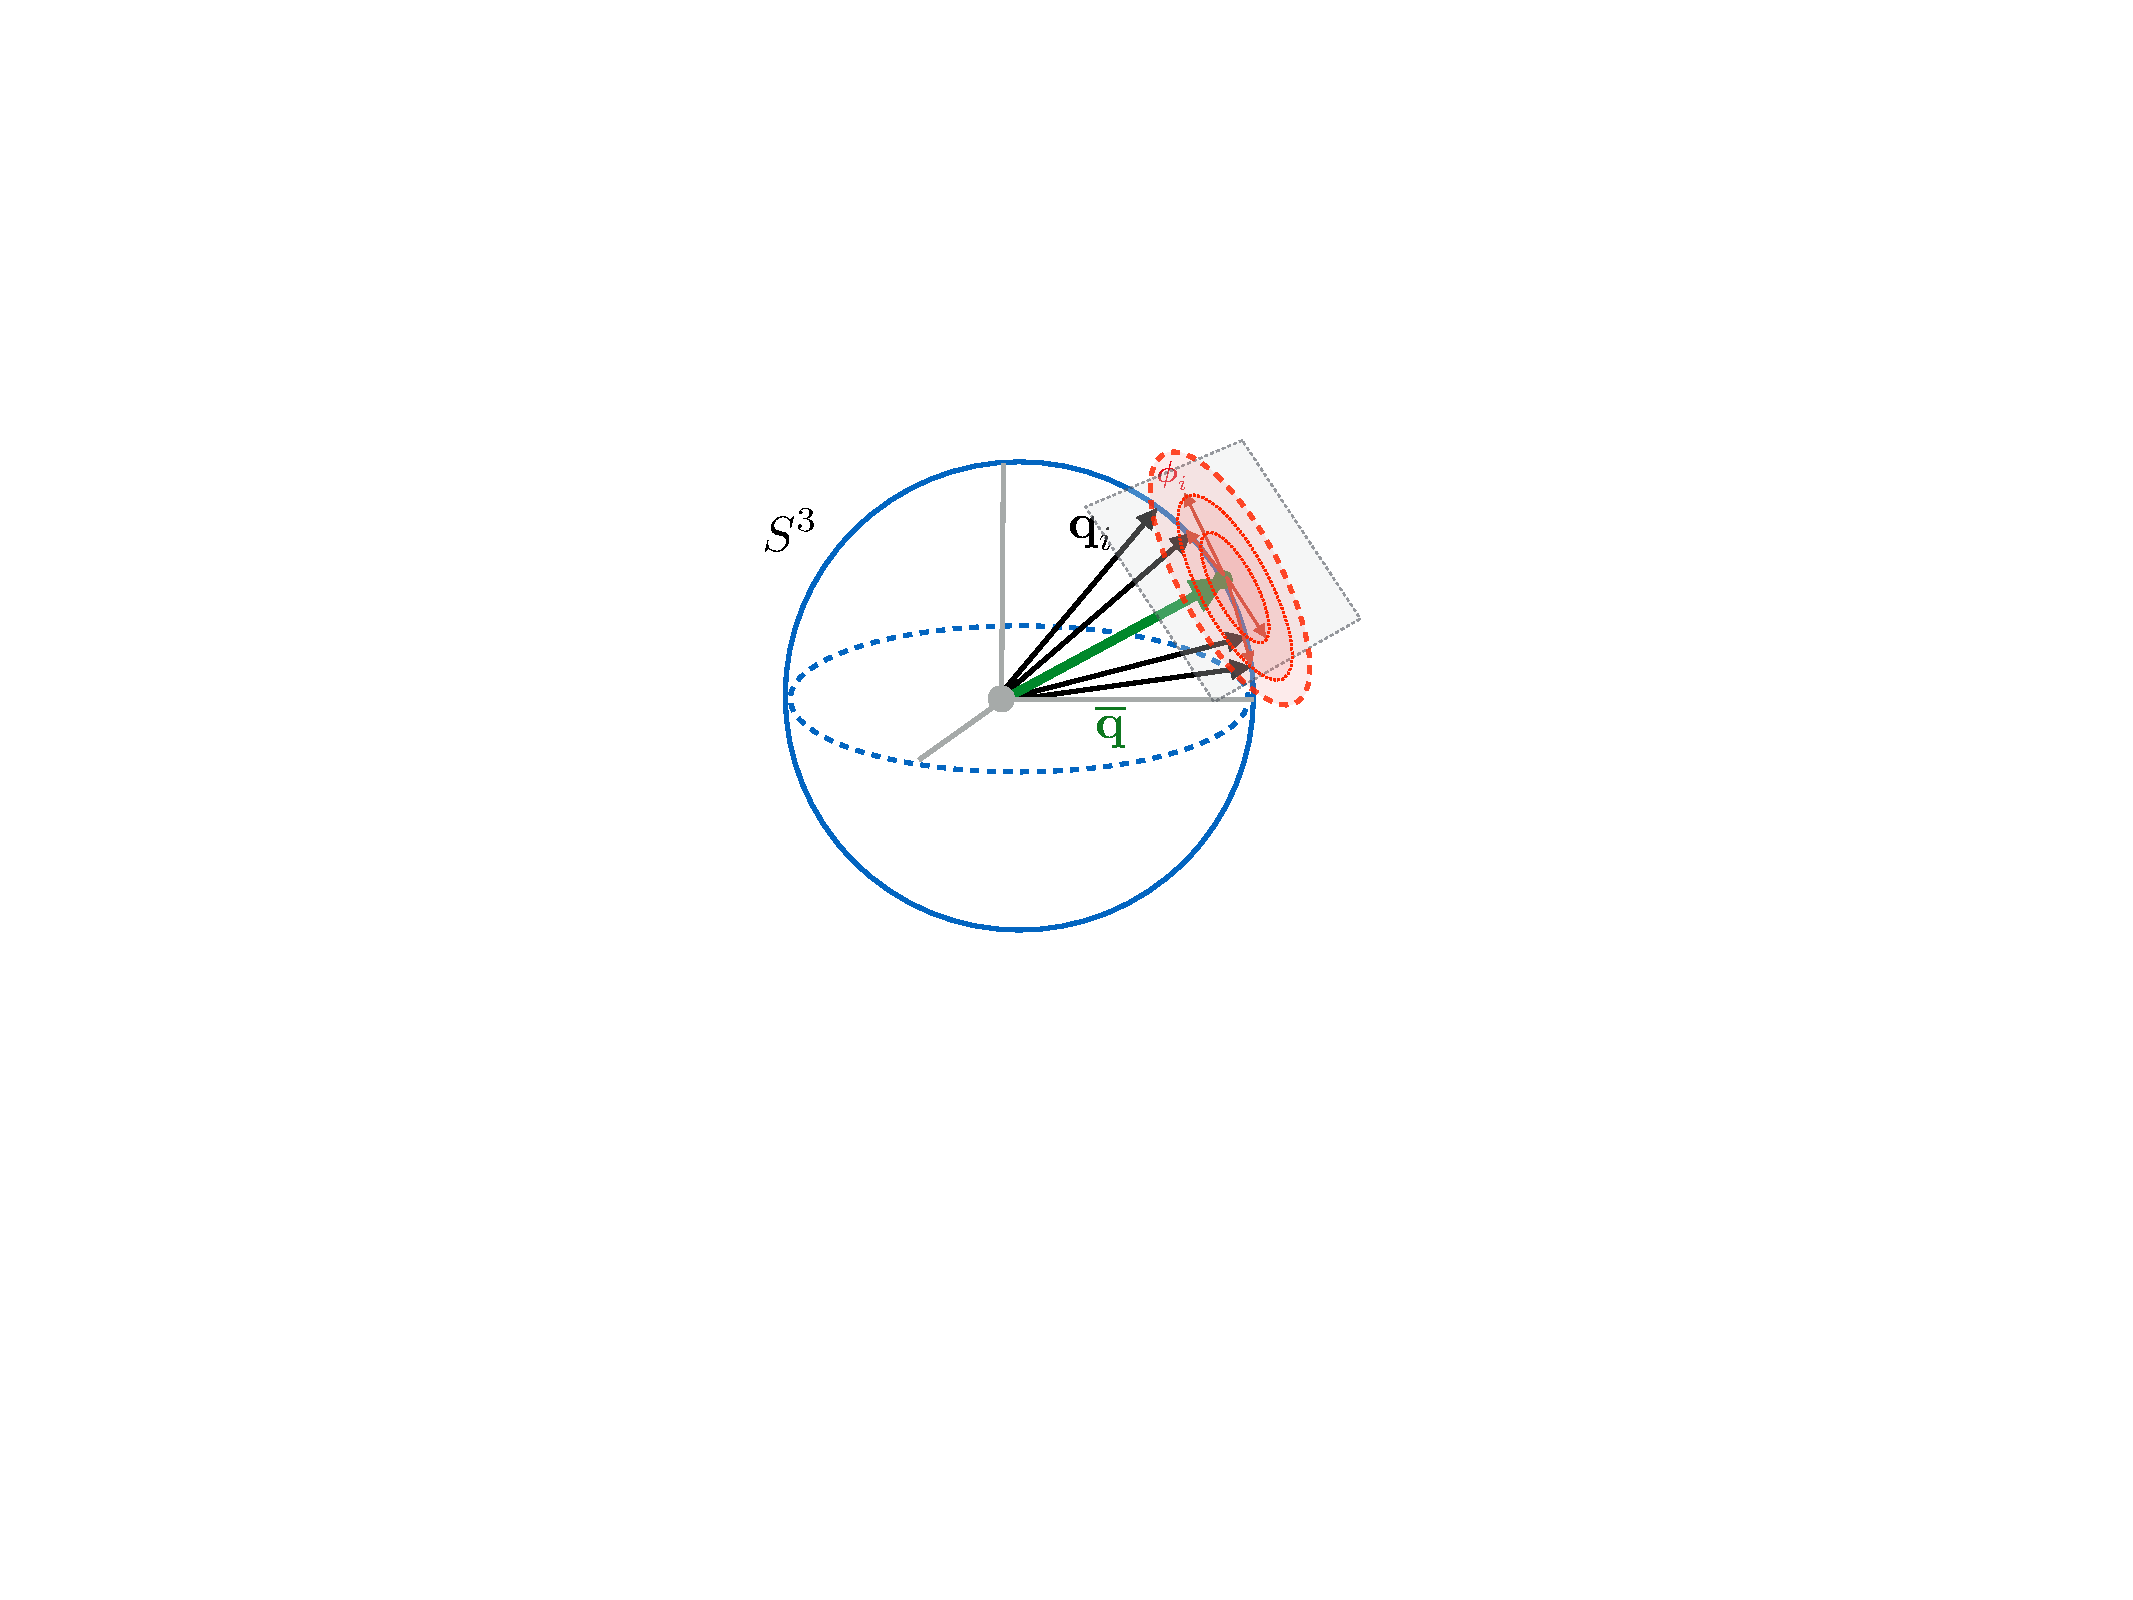
\includegraphics[width=0.33\textwidth]{math/quaternion_uncertainty.pdf}
  \end{center}
    \vspace{-20pt}
	\label{fig:math_quat_uncertainty}
	\caption{We can define uncertainty in the left tangent space of a mean element of a Lie group (here illustrated for unit quaternions).}
\end{wrapfigure} 


We can also use perturbation theory to implicitly define uncertainty on constrained manifolds (see \cite{Barfoot2014-ac} for a thorough discussion). 

Given a concentrated normal density, $\delta \TransformVector \sim \NormalDistribution{}(\Matrix{0}, \Matrix{\Sigma}_{6 \times 6})$, we can \textit{inject} this unconstrained density onto the Lie group through left perturbations about some mean:
\begin{align}
\Transform &= \MatExp{\delta \TransformVector} \Mean{\Transform} 
\end{align}
This allows us to keep track of a random variable, $\Transform$, by keeping its mean in group form, $\Mean{\Transform}$, while its second statistical moment is stored as a standard $6 \times 6$ covariance matrix, $\Matrix{\Sigma}$.

We can define an analogous density for rotation matrices given normal densities over rotation perturbations $\delta \RotationVector \sim \NormalDistribution{}(\Matrix{0}, \Matrix{\Sigma}_{3 \times 3})$,

\begin{align}
\Rotation &= \MatExp{\delta \RotationVector} \Mean{\Rotation}, 
\end{align}
and also, for unit quaternions,
\begin{align}
\quat &= \MatExp{\delta \RotationVector} \otimes \Mean{\quat} 
\end{align}
where $\otimes$ refers to the standard quaternion product operator \cite{Sola2017quaternion}. %\todo{Add discussion of banana density this induces for SE(3) and the impossibility of known position but unknown rotation}.



 
\chapter{Classical Visual Odometry}
\label{ch:vo}
\epigraph{Eventually, my eyes were opened, and I really understood nature.}{\textsc{Claude Monet}}

\begin{figure}[h!]
\begin{center}
		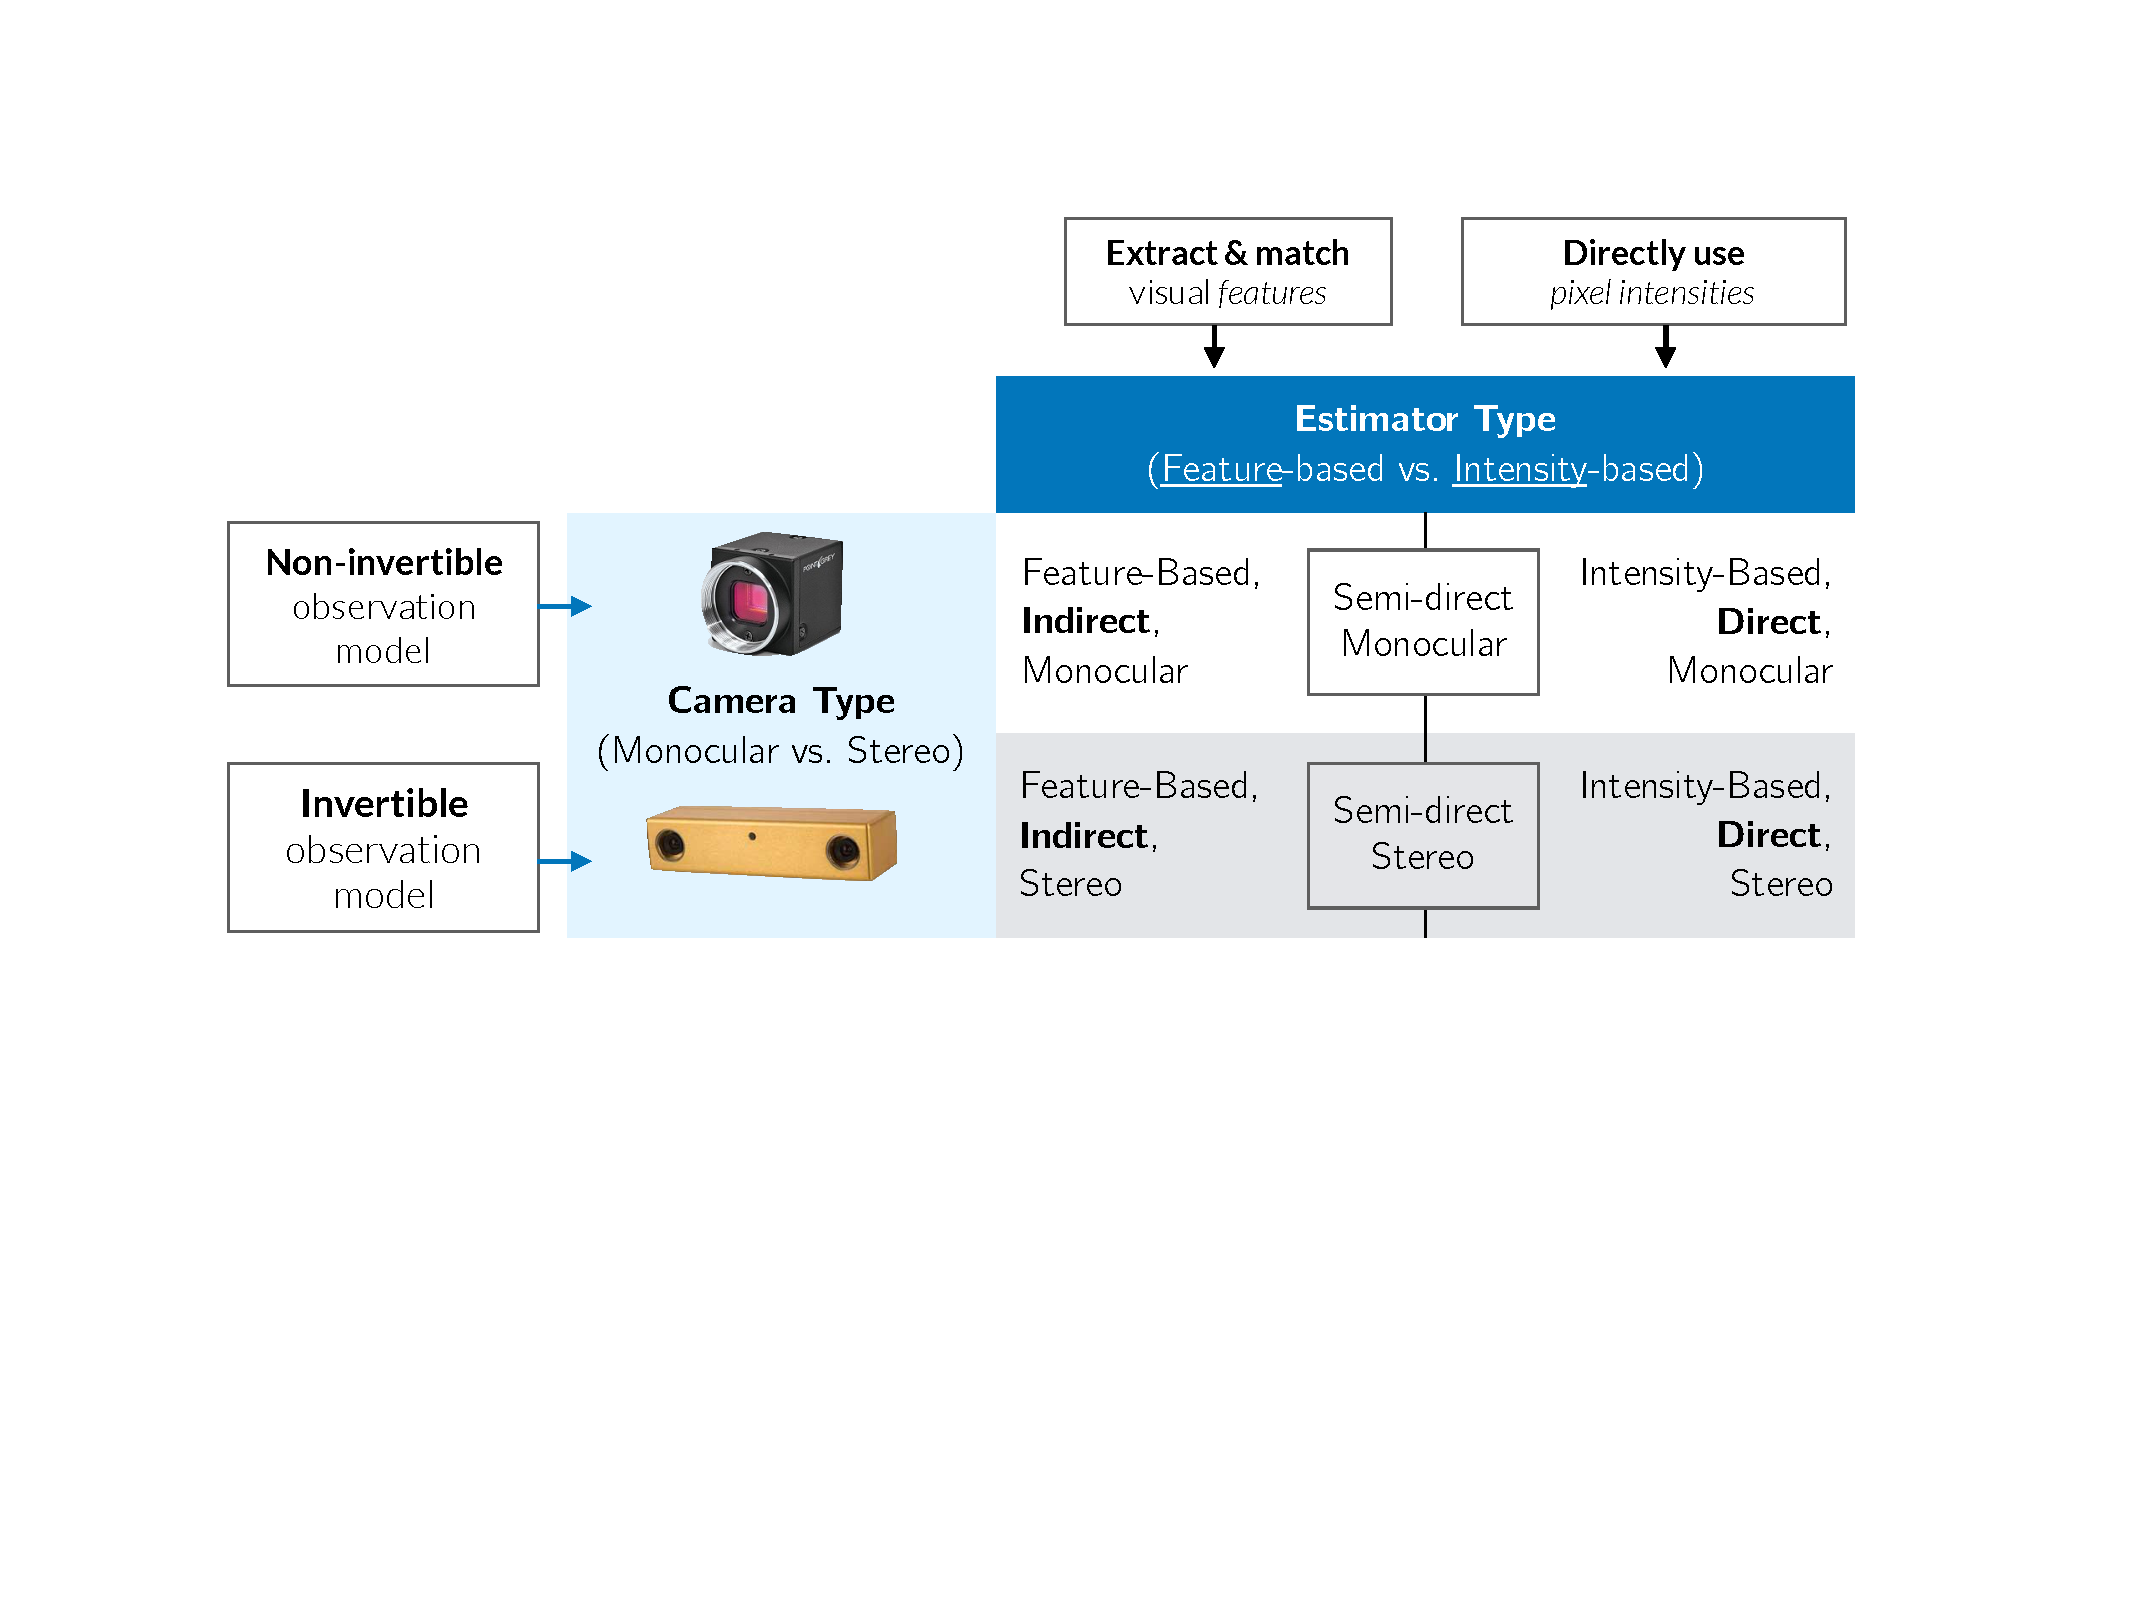
\includegraphics[width=0.95\textwidth]{classical-vo/vo_taxonomy.pdf}
		\caption{A taxonomy of different types of visual odometry.}
  	\label{fig:vo_taxonomy}
\end{center}
\end{figure}


Visual odometry (VO) has a rich history in mobile robotics and computer vision. As this dissertation largely deals with the improvement of a baseline visual odometry pipeline, we first outline the components of what we have chosen to be a canonical VO system. For a seminal tutorial on visual odometry and its more general cousin, visual SLAM, we refer the reader to two seminal papers: \cite{Scaramuzza2011-qr} and \cite{Cadena2016-ds}.

\section{A taxonomy of VO}

VO can be largely divided along two dimensions (c.f. \Cref{fig:vo_taxonomy}): the type of camera (monocular vs. stereo) and the type of data association (indirect, or feature-based vs. direct, or pixel intensity-based). 

\textbf{Monocular vs. Stereo:}
The first distinction is based on the type of camera used by the VO pipeline. Monocular VO methods use a single camera to infer motion and can use a single compact, low-power vision sensor. They do not require any extrinsic calibration but must rely on known visual cues or external information (e.g., wheel odometry, inertial measurements) to provide metric egomotion estimates. Conversely, stereo VO methods use a stereo camera to triangulate objects with metric scale. This allows stereo VO to provide metricaly-acurate egomotion estimates. However, stereo methods rely on accurate extrinsic calibration, and their ability to resolve depth is limited by the baseline distance between the stereo pair. 

\textbf{Direct vs. Indirect:}
The second distinction is based on the type of data association used to match sequential images. Direct methods make the assumption of brightness constancy, and attempt to \textit{directly} maximize the similarity of pixel intensities. Indirect methods, however, rely on image features detectors to extract a set of salient landmarks, and then match these landmarks across images (typically through some sort of invariant descriptor).

\section{A classical VO pipeline}

In this thesis, we apply our learned pseudo-sensors to a baseline stereo, indirect visual odometry pipeline largely based on the work of \cite{furgale_phd11}. We choose this baseline system for its computational efficiency and robustness. We briefly summarize the main components of the dpipeline here.

\begin{figure}[h!]
\begin{center}
		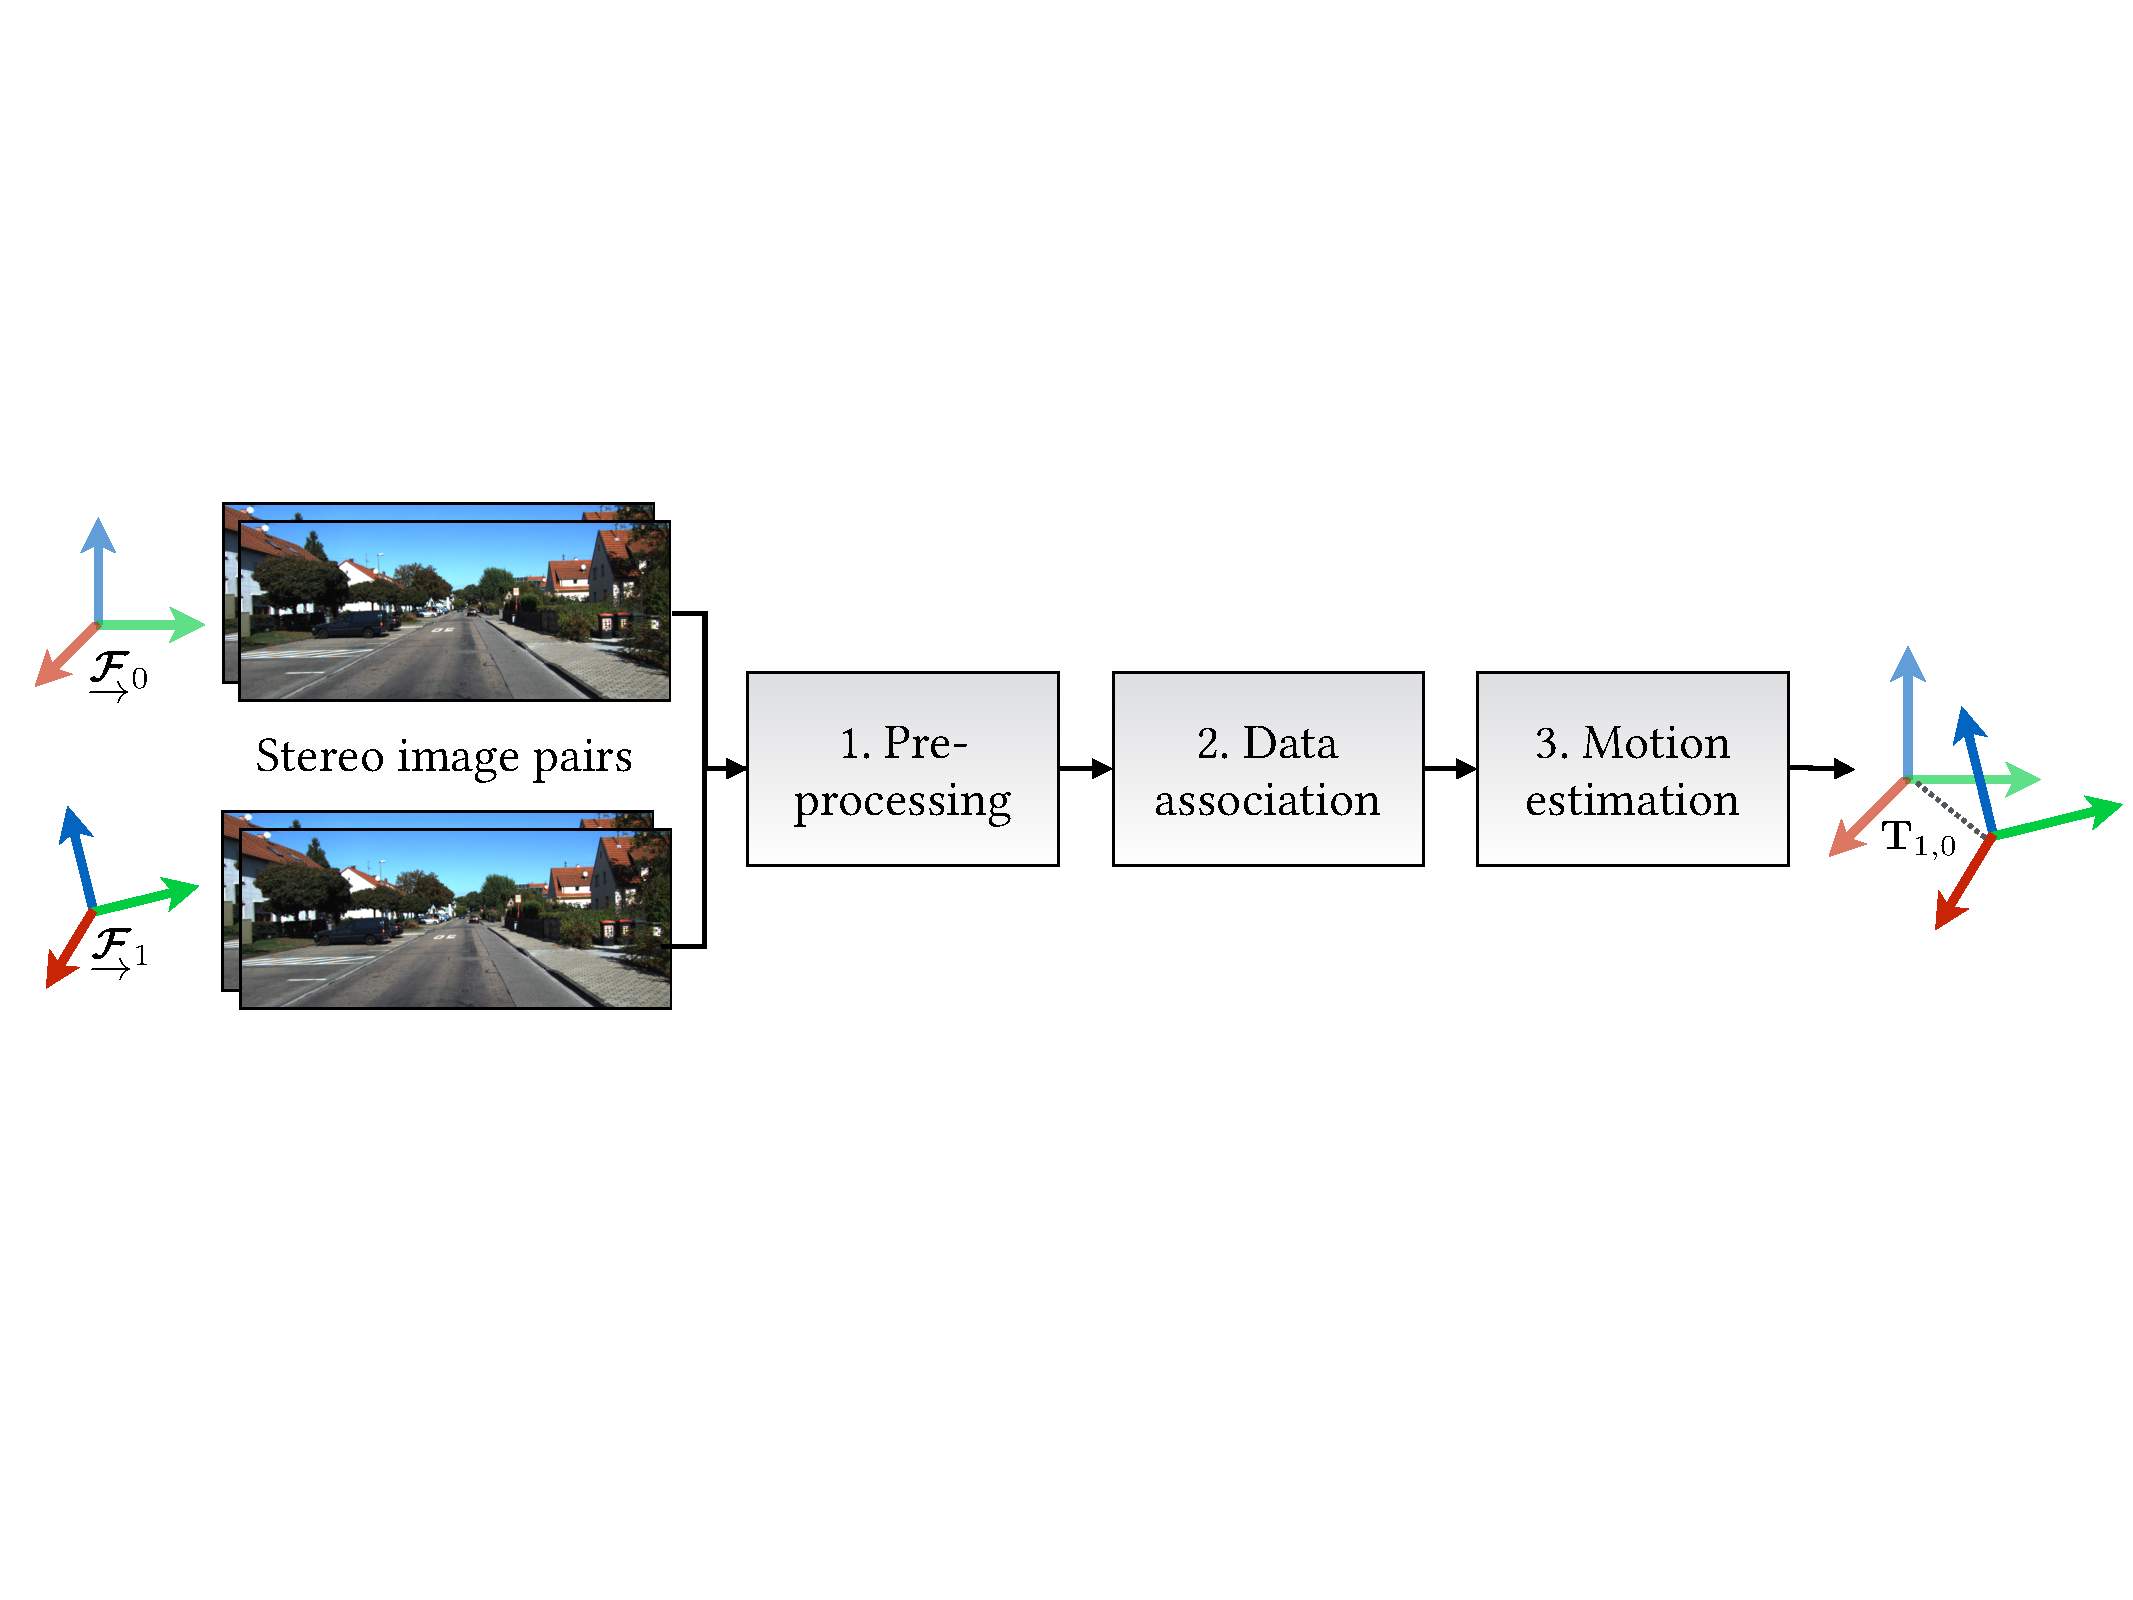
\includegraphics[width=0.98\textwidth]{classical-vo/stereo_vo_pipeline.pdf}
		\caption{A `classical' stereo visual odometry pipeline consists of several distinct components that have interpretable inputs and outputs.}
  	\label{fig:vo_stereo_vo_pipeline}
\end{center}
\end{figure}

\subsection{Preprocessing}


\begin{figure}[h!]
     \centering
     \begin{subfigure}[b]{0.48\textwidth}
         \centering
     		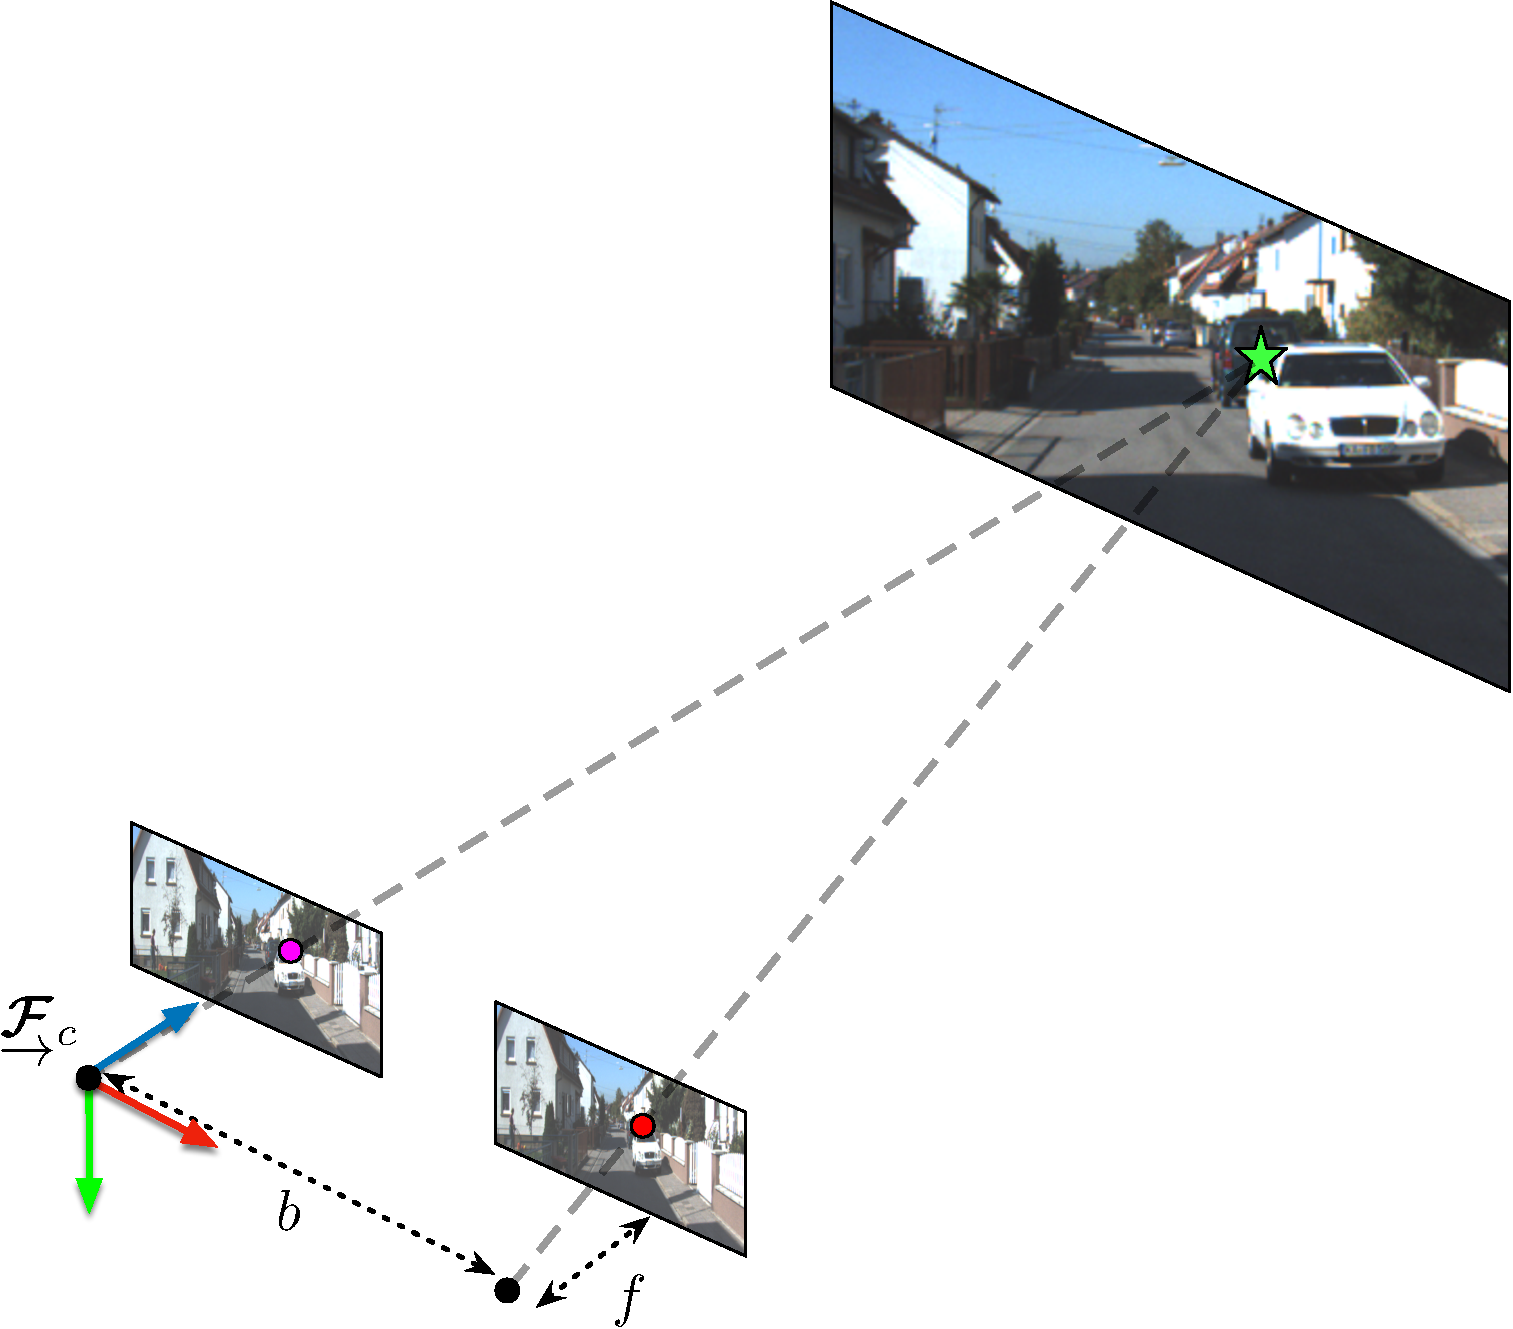
\includegraphics[width=0.98\textwidth]{classical-vo/stereo_camera}
			\caption{Ideal stereo camera.}
			 \label{fig:vo_stereo_camera}
     \end{subfigure}
     \hfill
     \begin{subfigure}[b]{0.48\textwidth}
         \centering
         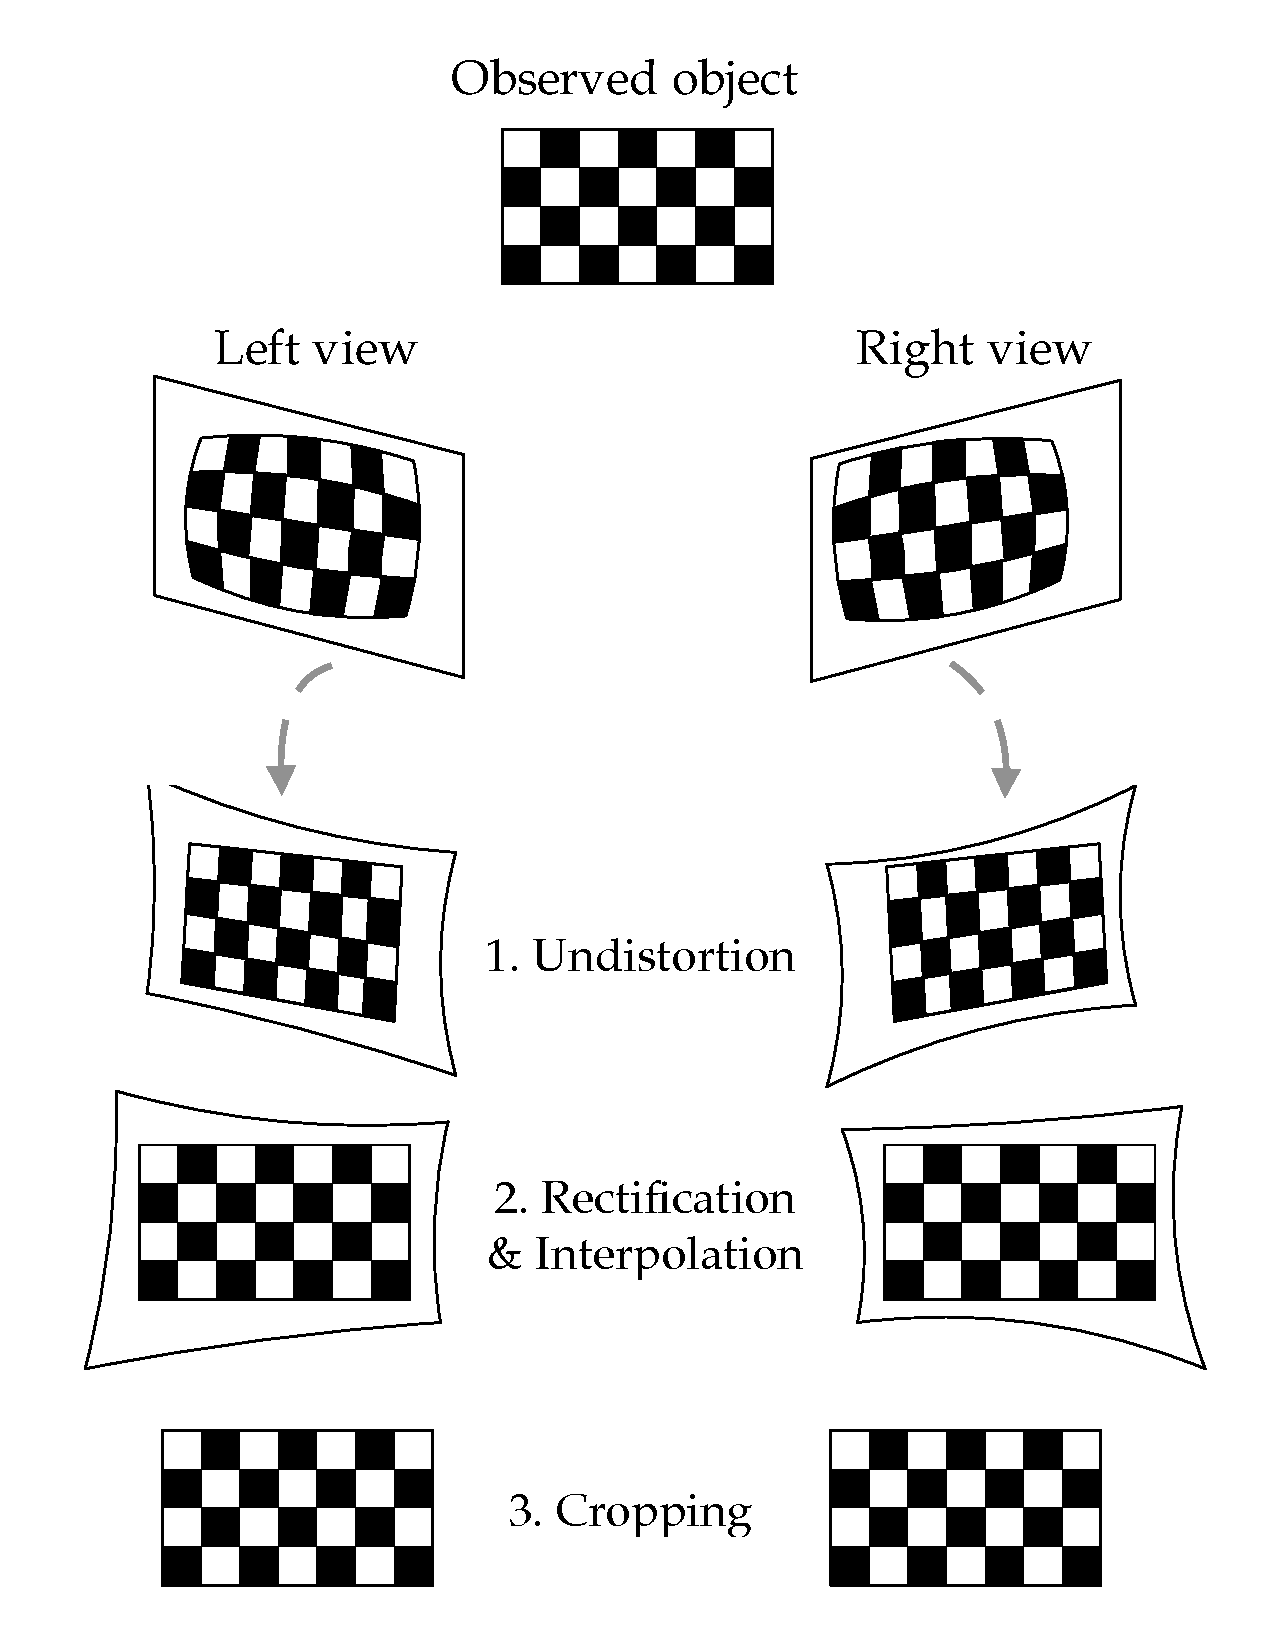
\includegraphics[width=0.75\textwidth]{classical-vo/stereo_rectification}
        \caption{Rectification and undistortion process. Figure adapted from \cite{florez2010}.}
         \label{fig:vo_undistort_recitfy}
	 \end{subfigure}
    \caption{Preprocessing components.}
        \label{fig:vo_preprocessing}
\end{figure}

During preprocessing, we use a lens model (assumed to be known apriori) to undistort each stereo image. Further, using the camera extrinsic parameters (also assumed to be known), we \textit{rectify} the stereo pair such that the images can be assumed to come from two cameras whose principal axes are parallel (\Cref{fig:vo_preprocessing}). Finally, we also assume that the stereo camera intrinsics are known a priori or compute them through a calibration process \citep{Furgale2013-sl}.

\subsection{Data association}

\subsubsection{Feature extraction and matching}

\begin{figure}[h!]
\begin{center}
		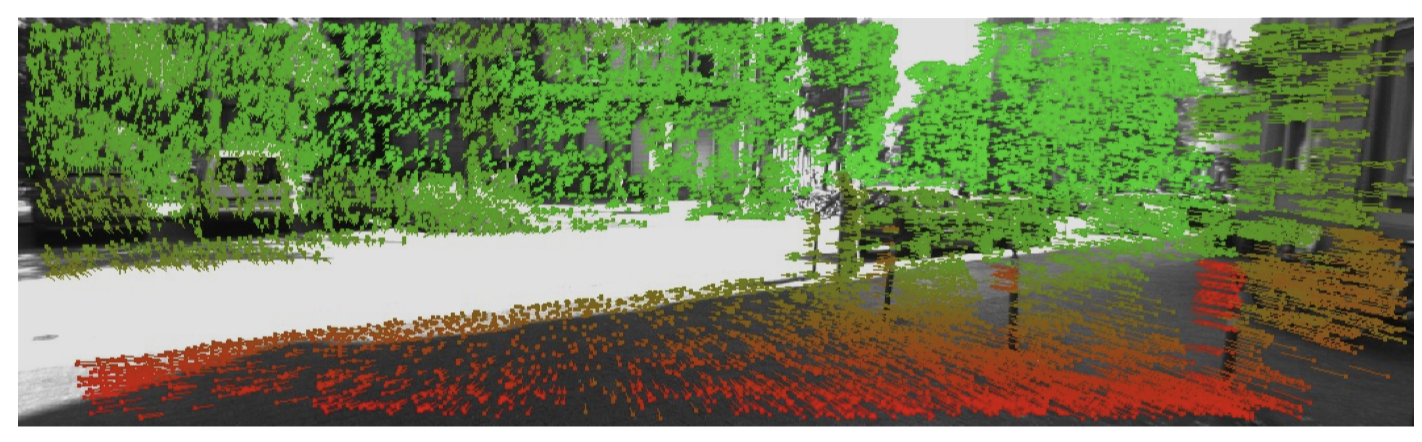
\includegraphics[width=0.88\textwidth]{classical-vo/libviso2_scan}
		\caption{Feature tracking using \texttt{libviso2}, taken from \cite{Geiger2011-xe}. Colours correspond to depth.}
  	\label{fig:vo_feature_tracking}
\end{center}
\end{figure}

In this thesis, we focus on indirect stereo visual odometry for its computational efficiency. Although a number of different types of indirect feature extraction and matching methods can be used towards this end, we choose to use the \texttt{viso2} \citep{geiger2011stereoscan} image feature extraction and matching algorithm. In \texttt{viso2}, features are extracted using blob and corner masks with non-minimum and non-maximum suppression. Unlike other features detectors that do not assume a particular camera motion, \texttt{viso2} assumes a smooth camera trajectory that permits fast matching through a simple sum-of-absolute-difference error metric of $11 \times 11$ windows of Sobel filter responses. Finally, features are matched across a stereo-pair and forward in time, to ensure that a single feature exists across two consecutive stereo camera poses. 

Each extract feature corresponds to a
point in space, expressed in homogeneous coordinates in the camera frame as
$\HomogeneousPoint{i}{t} := \Transpose{\bbm p_1 & p_2 & p_3 & p_4 \ebm} \in
\HomogeneousNumbers[3]$.  Given our intrinsics and extrinsic calibration parameters, our idealized stereo-camera model, $\ProjectionFunction$,
projects a landmark expressed in homogeneous coordinates into image space, so
that $\ImageLandmark{i}{t}$, the stereo pixel coordinates of landmark $i$ in the first camera pose at time $t$, is given
by 
\begin{equation}
	\ImageLandmark{i}{t} = \bbm u_l \\ v_l \\ u_r \\ v_r \ebm 
  = \ProjectionFunction(\HomogeneousPoint{i}{t}) 
  = \Matrix{M} \frac{1}{p_3}\HomogeneousPoint{i}{t},
\end{equation}
where
\begin{equation}
 \Matrix{M} = \bbm f & 0 & c_u & f \frac{b}{2} \\ 0 & f & c_v & 0 \\ f 
                        & 0 & c_u & -f\frac{b}{2} \\ 0 & f & c_v & 0 \ebm.
\end{equation}
Here, $\{c_u, c_v\}$, $\{f_u, f_v\}$, and $b$ are the principal points, focal
lengths and baseline of the stereo camera respectively. Note that in this
formulation, the stereo camera frame is centered between the two individual
lenses.  


\subsubsection{Outlier rejection}

To filter out any residual outlier matches, we use a three-point random sample consensus algorithm (RANSAC, \cite{FischlerRANSAC:1981}) based on an analytic solution to the six degree-of-freedom motion \citep{Umeyama1991-ws}.
  
\subsection{Motion solution}

To compute
$\Transform\in\text{SE}(3)$, the rigid transform between two subsequent stereo camera poses, we assume we have a set
of $N_t$ visual landmarks in each stereo pair at a time instance, $t$.

We triangulate landmarks in the first camera frame, $\ImageLandmark{i}{t}$, and re-project
them into the second frame, $\ImageLandmark{i}{t}'$. We model errors due to sensor noise
and quantization as a Gaussian distribution in image space with a covariance
$\ImageCovariance_{i,t}$ that may change for each feature or may be constant, $\ImageCovariance_{i,t} = \ImageCovariance$,
\begin{equation}
  p(\ImageLandmark{i}{t}' \vert \ImageLandmark{i}{t}, \Transform,
  \ImageCovariance_{i,t})
  =\NormalDistribution\left(\Vector{e}_{i,t}(\Transform); \Vector 0, \ImageCovariance_{i,t}\right), 
\end{equation}
where
\begin{equation}
 \Vector{e}_{i,t} = \ImageLandmark{i}{t}' - \ProjectionFunction( \Transform 
    \ProjectionFunction^{-1}( \ImageLandmark{i}{t} ) ).	
   \label{eq:image_error}
\end{equation}
  The maximum likelihood transform,
$\Transform^*$, is then given by 
\begin{equation}
  \Transform^* = \ArgMin{\Transform\in\text{SE}(3)}\sum_{i=1}^{N_t} 
  \Transpose{\Vector{e}_{i,t}} \ImageCovariance_{i,t}^{-1} \Vector{e}_{i,t}.
\end{equation}
This is a nonlinear least squares problem, and can be solved iteratively using
standard techniques. During iteration $n$, we represent the transform as the
product of an estimate $\Transform^{(n)}\in\text{SE}(3)$ and a perturbation
$\delta\Vector{\xi}\in\RealNumbers[6]$ represented in exponential
coordinates:
\begin{equation}
  \Transform = \exp{\left( \delta\Vector{\xi}^{\wedge}
  \right)} \Mean{\Transform}.
\end{equation}
Linearizing the transform for small perturbations $\delta\Vector{\xi}$
yields a linear least-squares problem:
\begin{equation}
\label{eq:vo_linleastsquares}
  \mathcal{L}(\delta \Vector{\xi}) = \frac{1}{2}\sum_{i=1}^{N_t} 
  \Transpose{\left(\Vector{e}_{i,t}^{(n)}
  - \Matrix J_{i,t}^{(n)} \delta\Vector{\xi}\right)}
\ImageCovariance_{i,t}^{-1}
 \left(\Vector{e}_{i,t}^{(n)}
 - \Matrix J_{i,t}^{(n)} \delta\Vector{\xi}\right)
  \end{equation}
Here, $\Matrix J_{i,t}^{(n)}$ is the Jacobian matrix of the reprojection error. 
Rearranging, we see the minimizing perturbation is the solution to a
linear system of equations:
\begin{equation}
  \delta\Vector{\xi}^{(n)} = 
  \left( \sum_{i=1}^{N_t} \Transpose{\Matrix J}_{i,t}
  \ImageLandmarkCovariance{}{}^{-1} \Matrix J_{i,t} \right)^{-1}
  \sum_{i=1}^{N_t} \Transpose{\Matrix J}_{i,t}
  \ImageCovariance_{i,t}^{-1} \Vector{e}_{i,t}^{(n)}. 
\label{eq:least-squares-iteration}
\end{equation}
We then update the estimated transform and proceed to the next iteration,
\begin{equation}
  \Transform^{(n+1)} = \MatExp{\delta\Vector{\xi}^{(n)}} \Transform^{(n)}. \label{eq:update}
\end{equation}
There are many reasonable choices for both the initial transform
$\Transform^{(0)}$ and for the conditions under which we terminate
iteration. We initialize the estimated transform to identity, and iteratively
perform the update given by \cref{eq:update} until we see a relative change in
the squared error of less than one percent after an update. 

%\newpage
%\section{Pose Graph Optimization}
%
%\begin{wrapfigure}{r}{0.4\textwidth}
%  \vspace{-20pt}
%  \begin{center}
%	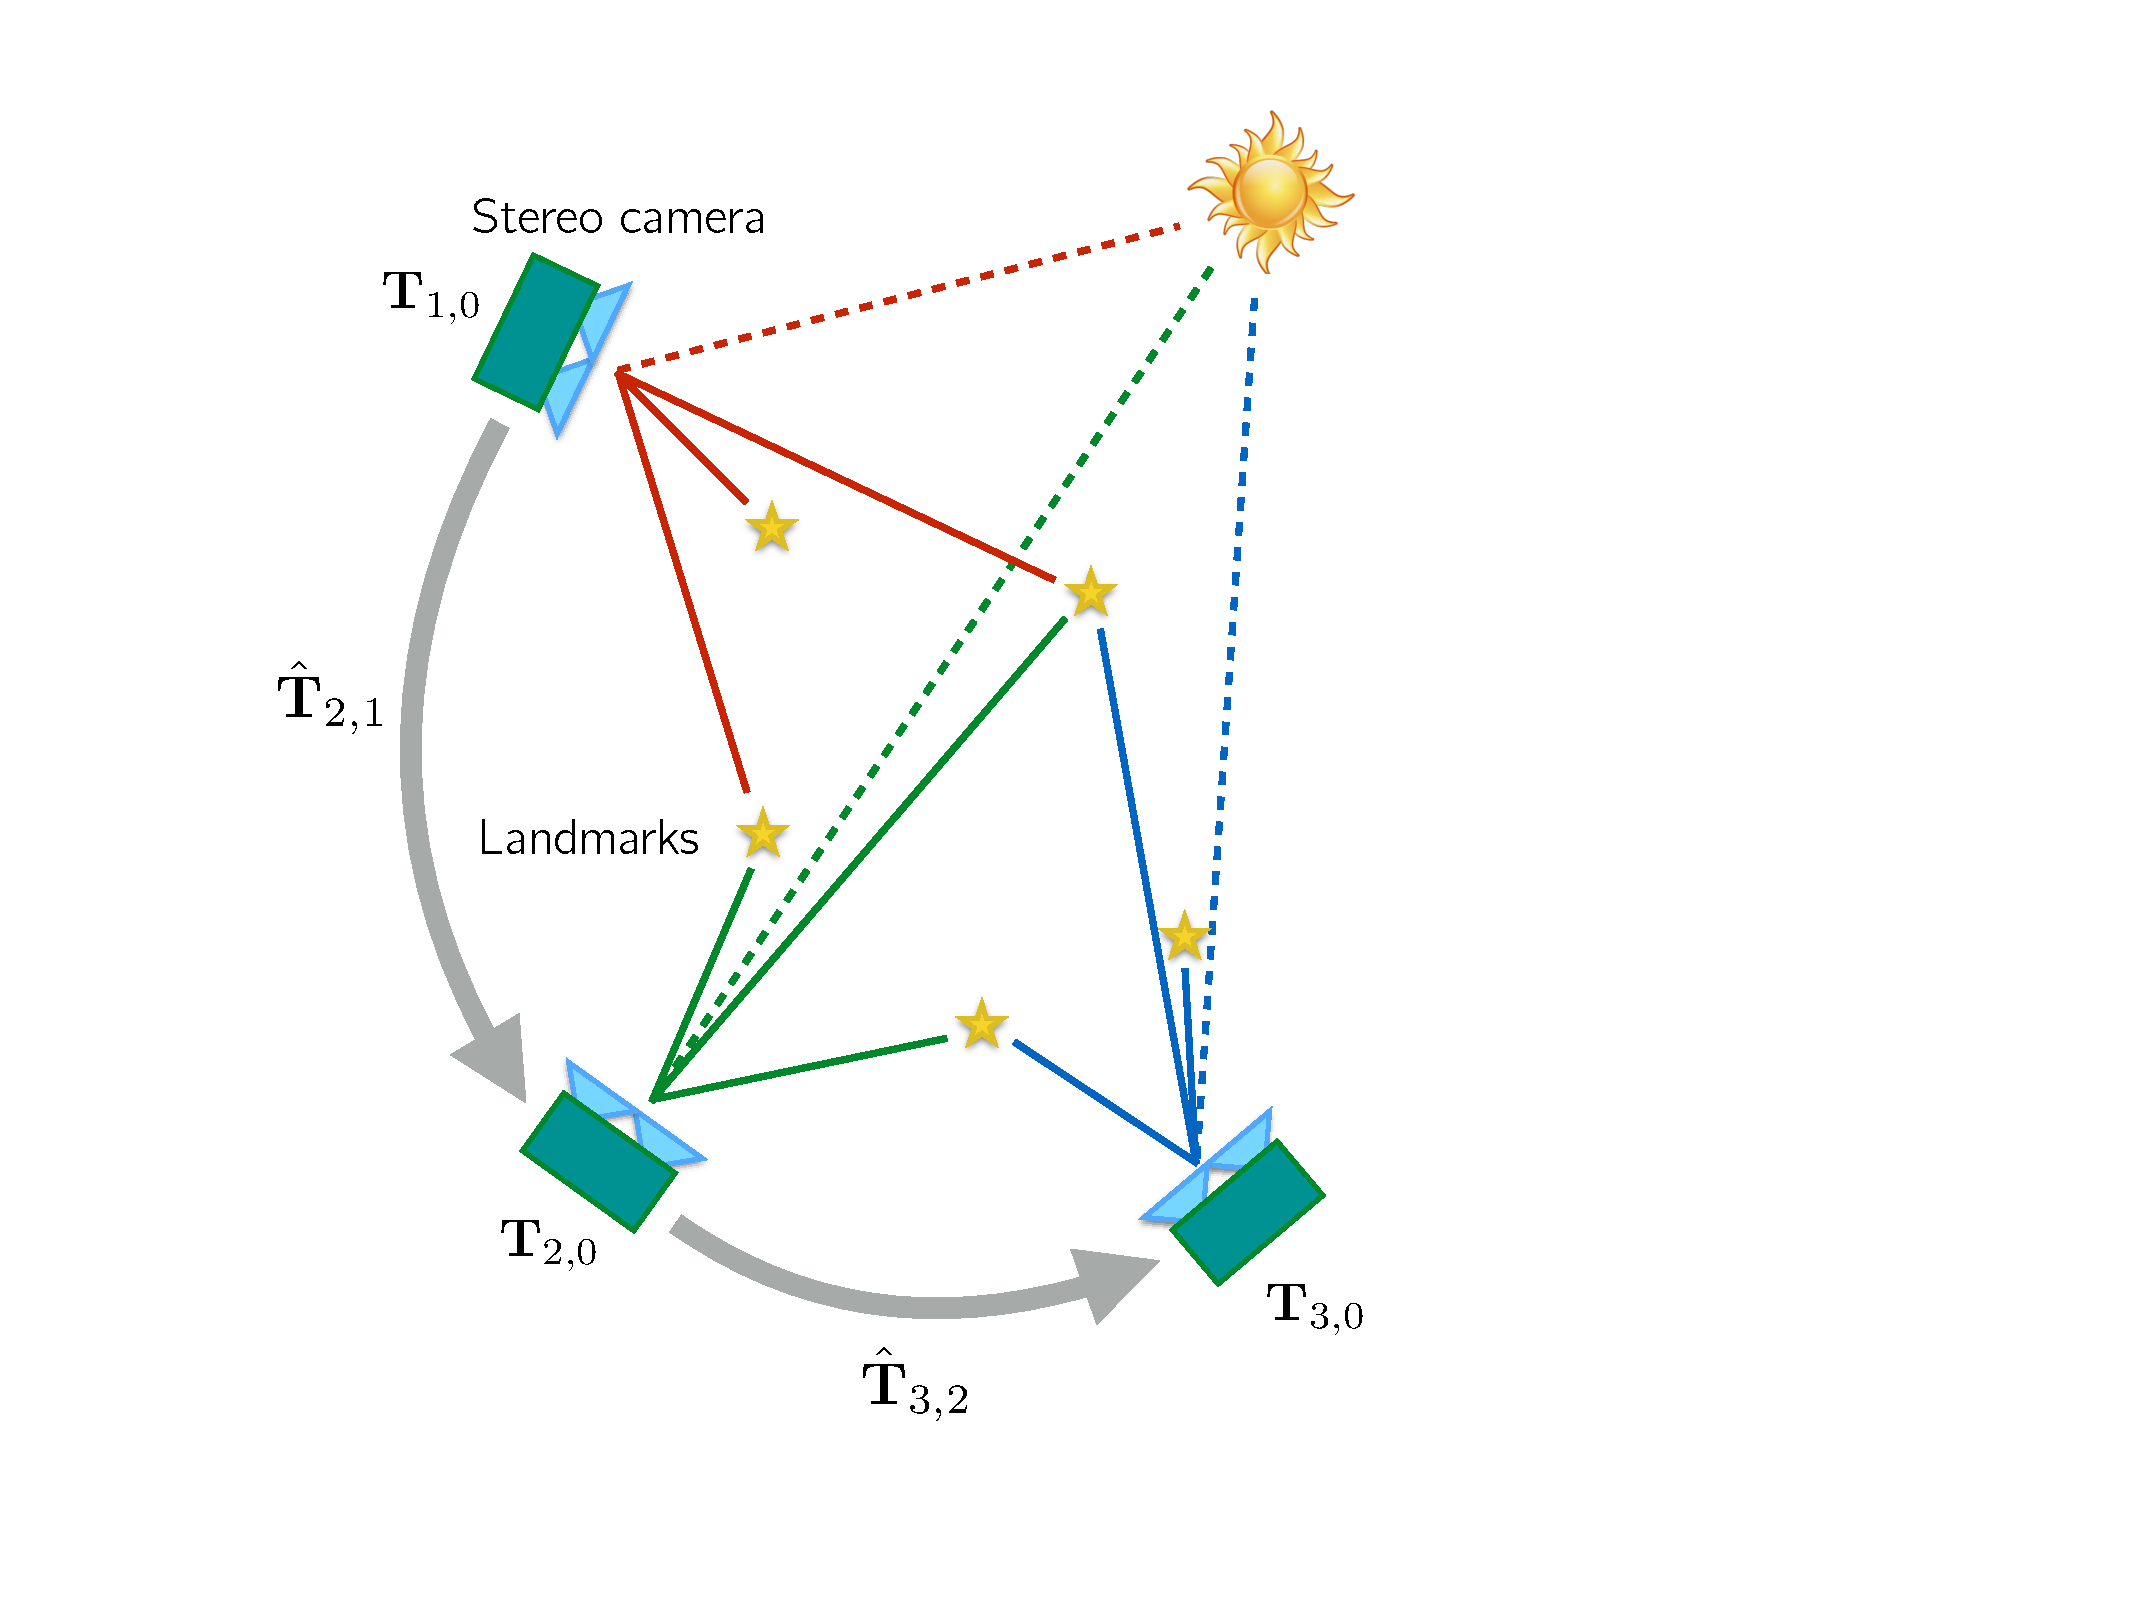
\includegraphics[width=0.38\textwidth]{classical-vo/pose_graph.pdf}
%  \end{center}
%    \vspace{-20pt}
%	\label{fig:math_pose_graph}
%	\caption{The formulation of pose graph relaxation can incorporate different probabilistic \textit{factors} that constrain each camera pose.}
%\end{wrapfigure} 
%
%
%we fused our probabilistic rotation regression with classical stereo visual odometry using pose graph relaxation implemented with the help of a Python-based factor graph library which we will publicize after the review process. Using that framework, we solved
%\begin{align}
%	\Transform_{1,w}^*, \Transform_{2,w}^* &= \ArgMin{\Transform_{1,w}, \Transform_{2,w}\in\text{SE}(3)}\mathcal{L}(\Estimate{\Transform}_{2,1}, \Estimate{\Rotation}_{2,1}) \\ & = \ArgMin{\Transform_{1,w}, \Transform_{2,w}\in\text{SE}(3)} \Vector{\xi}_\text{1,2}^T \Matrix{\Sigma}^{-1}_\text{vo} \Vector{\xi}_\text{1,2} + \Vector{\phi}_\text{1,2}^T \Matrix{\Sigma}^{-1}_{\text{hn}} \Vector{\phi}_\text{1,2} 
%\end{align}
%where
%\begin{equation}
%	\Vector{\xi}_\text{1,2} =  \MatLog{\left(\Transform_{2,w} \Transform_{1,w}^{-1} \right)\Estimate{\Transform}_{2,1}^{-1}},
%\end{equation}
%\begin{equation}
%	\Vector{\phi}_\text{1,2} =  \MatLog{\left(\Rotation_{2,w} \Rotation_{1,w}^{T} \right)\Estimate{\Rotation}_{2,1}^{T}},
%\end{equation}
%and $\Estimate{\Transform}_{2,1}$, $\Matrix{\Sigma}_\text{vo}$ and $\Estimate{\Rotation}_{2,1}$, $\Matrix{\Sigma}_{\text{hn}}$ were provided by our classical estimator and the HydraNet network respectively. Note that $\Matrix{\Sigma}_{\text{hn}} \in \Real^{3 \times 3} \geq 0$ while $\Matrix{\Sigma}_{\text{vo}} \in \Real^{6 \times 6} \geq 0 $. We also overload the logarithm function, $\MatLog{\cdot}$ to represent both $\LieGroupSE{3}$ and $\LieGroupSO{3}$ logarithmic maps as necessary. To account for gauge freedom, we fixed the first transformation to identity, $\Transform_{1,w} = \IdentityMatrix$, and initialized $\Transform_{2,w}$ to  $\Estimate{\Transform}_{2,1}$.  After convergence, we composed the final frame-to-frame estimate as $ \Transform_{2,1}^* =  \Transform_{2,w}^*  \left(\Transform_{1,w}^*\right)^{-1} = \Transform_{2,w}^*$.
%



\section{Robust Estimation}
Since \cref{eq:vo_linleastsquares} assigns cost values that grow quadratically with measurement error, it is very sensitive to outlier measurements.
A common solution to this problem is to replace the $L_2$ cost function with one that is less sensitive to large measurement errors \citep{MacTavish2015-wt}.
These robust cost functions are collectively known as M-estimators, and many variants exist. Each uses a re-weighting function, $\rho(\cdot)$,

\begin{equation}
  \Transform^* = \ArgMin{\Transform\in\text{SE}(3)}\sum_{i=1}^{N_t} 
  \rho\left(\Transpose{\Vector{e}_{i,t}} \ImageCovariance_{i,t}^{-1} \Vector{e}_{i,t}\right) = \ArgMin{\Transform\in\text{SE}(3)}\sum_{i=1}^{N_t} 
  \rho(\epsilon_i),
\end{equation}

where. given a parameter $c$, some common examples include:

\begin{align}
\rho(\epsilon) &= \left\{  	\begin{array}{ll}
		 \frac{c^2}{2} \log{\left(1 + \frac{\epsilon^2}{c^2}\right)}   & \mbox{Cauchy,} \\
		 \frac{1}{2} \frac{\epsilon^2}{c^2 + \epsilon^2}  & \mbox{Geman-McClure \citep{geman1992nonlinear},} \\
		 \\
		\left\{  	\begin{array}{ll}  \frac{\epsilon^2}{2} & \mbox{if} \Norm{\epsilon} < c \\
										c\Norm{\epsilon} - \frac{c^2}{2} & \mbox{if} \Norm{\epsilon} \geq c \end{array}
																						 \right.   & \mbox{Huber \citep{huber1964robust}.} \\
	\end{array}
	\right.
\end{align}




\section{Outstanding Issues}
There are several outstanding limitations of classical visual odometry pipelines that we can address with learned pseudo-sensors. 

\begin{table}[h!]
	\caption{\textbf{Data efficiency vs. computational efficiency}}	\begin{threeparttable}
	\begin{tabular}{m{0.68\textwidth}m{0.28\textwidth}}
		\toprule
		\textbf{Synopsis} & \textbf{Addressed by} \\ \midrule  
		Classical VO pipelines face a difficult-to-optimize trade-off between using all of the information contained within image and while still remaining computationally tractable.  & PROBE, DPC-Net, Sun-BCNN, HydraNet \\
		& \\
		\bottomrule
	\end{tabular}
\end{threeparttable}
\end{table}


\begin{table}[h!]
	\caption{\textbf{Systematic bias}}
	\begin{threeparttable}
	\begin{tabular}{m{0.68\textwidth}m{0.28\textwidth}}
		\toprule
		\textbf{Synopsis} & \textbf{Addressed by} \\ \midrule  
		Stereo visual odometry can incur systematic bias through poor extrinsic or intrinsic calibration, stereo triangulation errors, poor feature \textit{spread} (i.e., concentration of features on one side of an image), and poor data association due self-similar textures. &  DPC-Net \\
		& \\
		\bottomrule
	\end{tabular}
\end{threeparttable}
\end{table}


\begin{table}[h!]
	\caption{\textbf{Homoscedastic uncertainty}}
	\begin{threeparttable}
	\begin{tabular}{m{0.68\textwidth}m{0.28\textwidth}}
		\toprule
		\textbf{Synopsis} & \textbf{Addressed by} \\ \midrule  
		Stationary, homoscedastic noise in observation models can often reduce the consistency and accuracy of state estimates. This is especially true for complex, inferred measurement models. In visual data, inferred visual observations can be degraded not only due to sensor imperfections (e.g. poor intrinsic calibration, digitization effects, motion blur), but also as a result of the observed environment (e.g. self-similar scenes, specular surfaces, textureless environments). &  PROBE, Sun-BCNN, HydraNet \\
		& \\
		\bottomrule
	\end{tabular}
\end{threeparttable}
\end{table}

%
%
%\textbf{Adaptation to new environments}
%
%\begin{table}[h!]
%	\begin{threeparttable}
%	\begin{tabular}{m{0.68\textwidth}m{0.28\textwidth}}
%		\toprule
%		\textbf{Synopsis} & \textbf{Addressed by} \\ \midrule  
%		Traditional VO pipelines do little to adapt to new environments.
%. &  PROBE-GK, DPC-Net, HydraNet \\
%		& \\
%		\bottomrule
%	\end{tabular}
%\end{threeparttable}
%\end{table}


\chapter{Predictive Robust Estimation}
\label{ch:probe}
\epigraph{Information is the resolution of uncertainty.}{Claude Shannon}

\section{Introduction}

\begin{figure*}[h!]
\centering
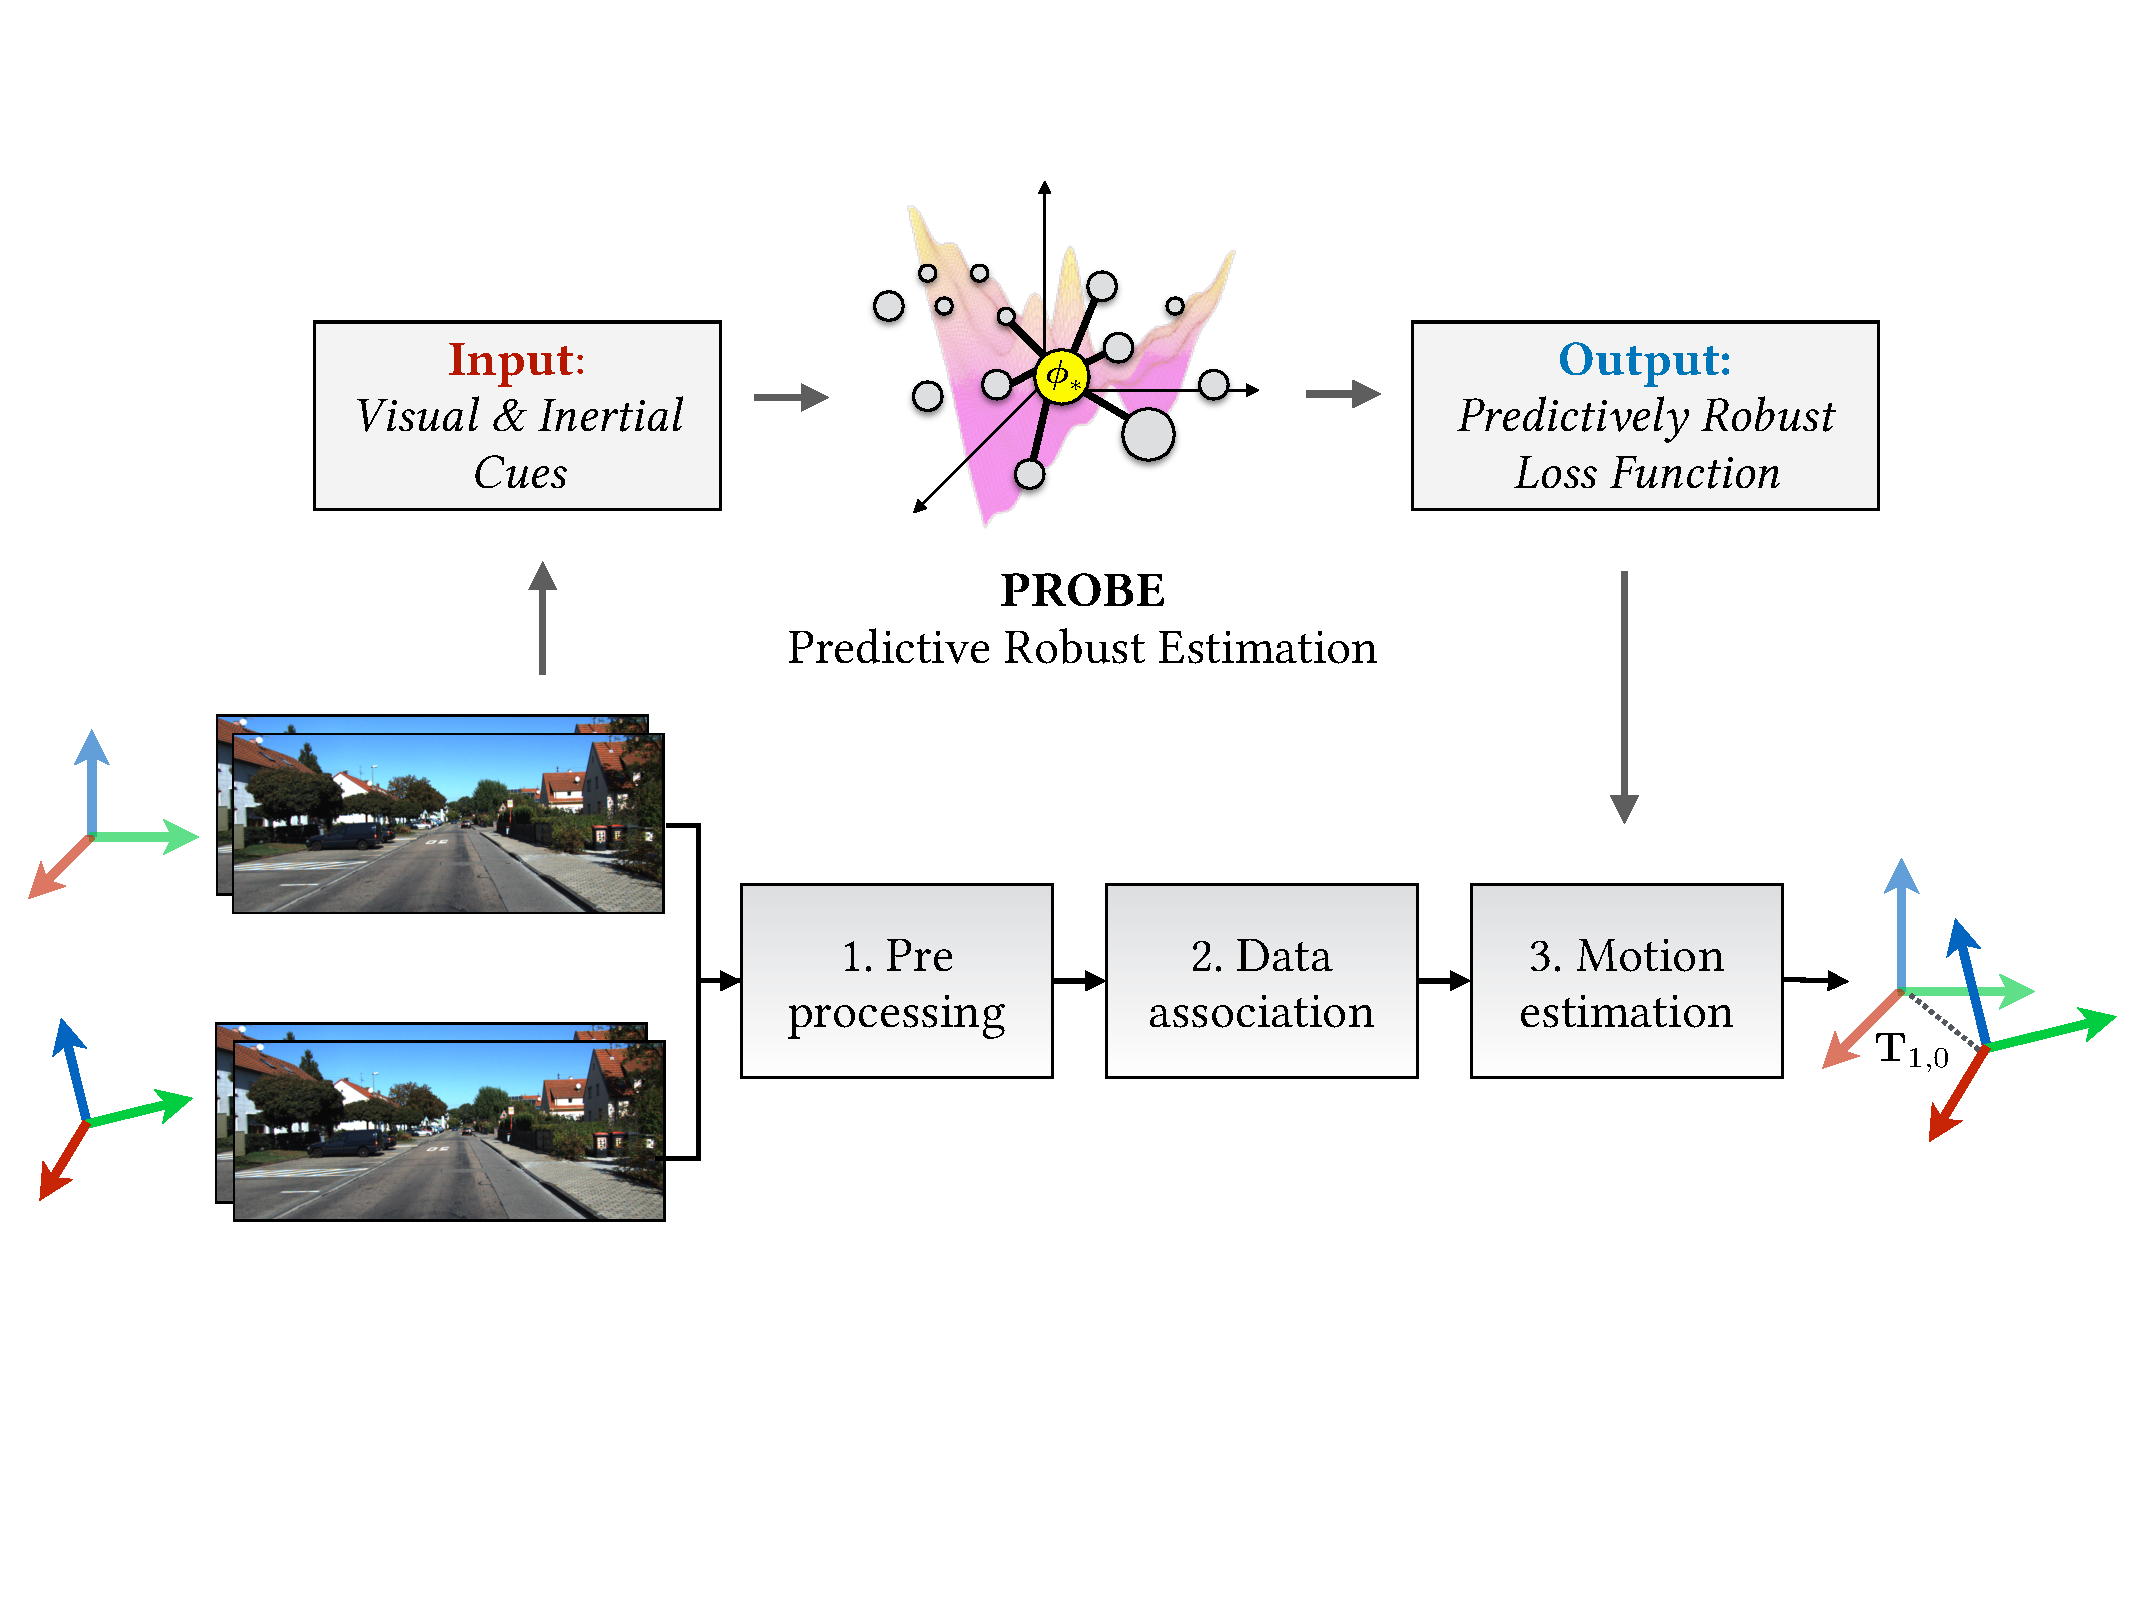
\includegraphics[width=0.8\textwidth]{probe.pdf}
 \caption{PROBE builds a predictive noise model for stereo visual odometry.}
 \label{fig:probe_intro_fig}
\end{figure*}

The first pseudo-sensor we present is a technique we call PRedictive ROBust Estimation, or PROBE. This approach uses non-parametric learning to build a model for anisotropic observation covariances for a stereo visual odometry pipeline. Namely, we apply the method of Generalized Kernels to a Bayesian treatment of covariance estimation. We show that by assuming a particular covariance prior over re-projection errors, we can then naturally derive a robust least squares objective that resembles the widely-used Cauchy loss. The parameters of this robust loss are predicted (hence \textit{predictive} robust estimation) for each error term as a function of a prediction space that we define.

PROBE was initially published as a simpler non-Bayesian technique that learned isotropic covariances through a k-nearest-neighbours approach (see Appendix \ref{app:appendix_probe_knn} for more details).  The following two publications summarize this initial technique:
\begin{enumerate}
\item \bibentry{2015_Peretroukhin_PROBE}
\item \bibentry{2015_Peretroukhin_Get}
\end{enumerate}

We significantly extended this technique to full anisotropic covariances and generalized kernels in the following publication:
\begin{enumerate}
\item \bibentry{Peretroukhin2016-om}	.
\end{enumerate}

We will present this latter technique in this chapter.


%\begin{wrapfigure}{r}{0.5\textwidth}
%    \centering
%      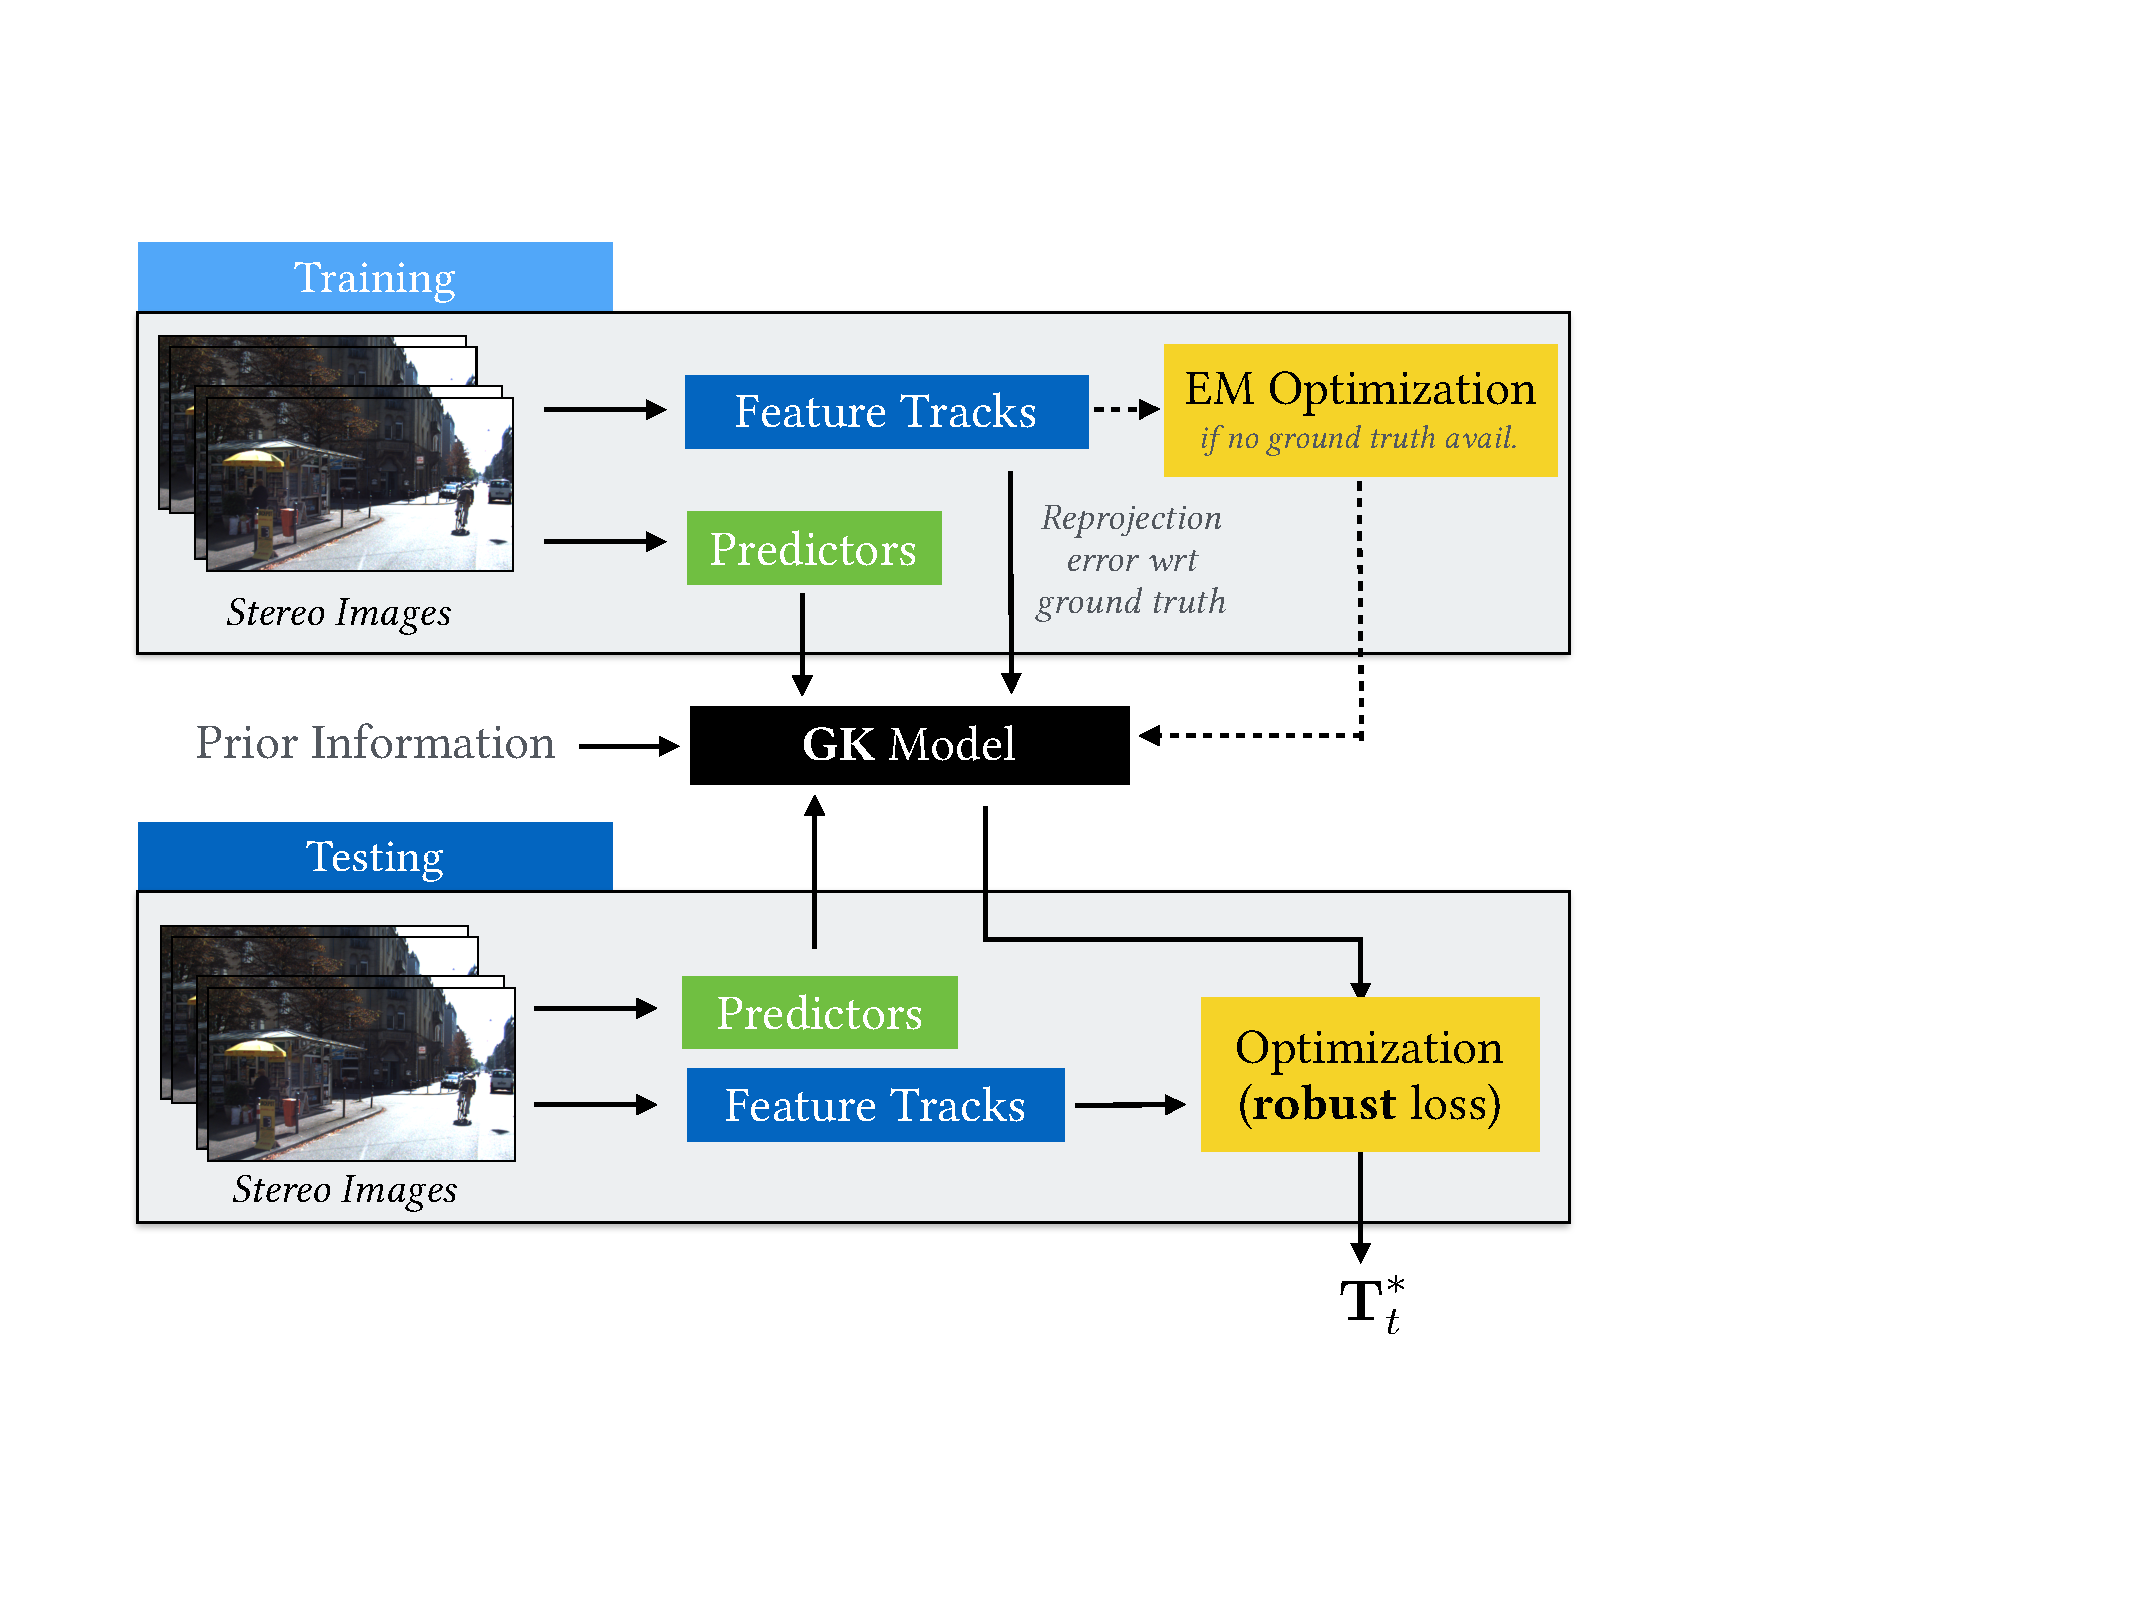
\includegraphics[width=0.5\textwidth]{probe-gk/system_overview}
%      \caption{PROBE builds a predictive noise model for stereo visual odometry.}
%        \vspace{-1em}
%    \label{fig:probe_gk_system}
%\end{wrapfigure}

\section{Motivation}

Robot navigation relies on an accurate quantification of sensor noise or uncertainty in order to produce reliable state estimates.
In practice, this uncertainty is often fixed for a given sensor and experiment, whether by automatic calibration or by manual tuning.
Although a fixed measure of uncertainty may be reasonable in certain static environments, dynamic scenes frequently exhibit many effects that corrupt a portion of the available observations.
For visual sensors, these effects include, for example, self-similar textures, variations in lighting, moving objects, and motion blur. 
Further, there may be useful information available in these observations that would normally be rejected by a fixed-threshold outlier rejection scheme. 
Ideally, we would like to retain some of these observations in our estimator, while still placing more trust in observations that do not suffer from such effects.


\section{Related Work}


There is a large and growing body of work on the problem of deriving accurate,
consistent state estimates from visual data.  Although our approach to noise
modelling is applicable in other domains, for simplicity we focus our attention
on the problem of inferring egomotion from features extracted from sequential
pairs of stereo images; see \citet{sunderhauf2007stereo} for a survey of
techniques. The spectrum of alternative approaches to visual state estimation
include monocular techniques, which may be feature-based
\citep{Scaramuzza2011-qr}, direct \citep{irani2000direct}, or semi-direct
\citep{forster2014svo}. 

Apart from simply rejecting outliers, a number of recent approaches attempt to
select the optimal set of features to produce an accurate localization estimate
from tracked visual features. For example, \citet{Tsotsos2015} amend Random
Sample Consensus (RANSAC) with statistical hypothesis testing to ensure that tracked visual features have normally distributed residuals before including them in
the estimator. Unlike our predictive approach, their technique relies on the availability of feature tracks, and requires scene overlap to work continuously. In a different
approach, \Citet{Zhang2015} choose an optimally observable feature subset for a
monocular SLAM pipeline by selecting features with the highest \textit{informativeness} - a measure calculated based on the observability of the SLAM subsystem. Observability, however, is governed by the 3D location of the features, and therefore cannot predict systematic feature degradation due to environmental or sensor-based effects. 


\section{Predictive Robust Estimation for VO}

%However, not all features are created equal; most feature-based methods rely on
%random sample consensus algorithms \citep{fischler1981random} to partition the extracted features
%into inliers and outliers, and perform estimation based only on inliers. It is
%common to guard against misclassifying an outlier as an inlier by using robust
%estimation techniques, such as the Cauchy costs employed in
%\citet{kerl2013robust} or the dynamic covariance scaling devised
%by \citet{Burgard:ii}. These approaches, often grouped under the title of M-estimation, aim to maintain a quadratic influence
%of small errors, while reducing the contribution of larger errors. The
%robustness and accuracy of feature-based visual odometry often hinges on the
%tuning of the parameters of inlier selection and robust estimation. Performance
%can vary significantly from one environment to the next, and most algorithms require
%careful tuning to work in a given environment. 

We present a principled, data-driven way to build a noise model
for visual odometry. We combine our previous work
on predictive robust estimation with isotropic covariances (Appendix \ref{app:appendix_probe_knn}) with work on covariance estimation
\citep{VegaBrown:2013fv} to formulate a predictive robust estimator for a
stereo visual odometry pipeline. We frame the traditional non-linear least
squares optimization problem as a problem of maximum likelihood estimation with
a Gaussian noise model, and infer a distribution over the covariance matrix of
the Gaussian noise from a predictive model learned from training data. This
results in a Student's~$t$ distribution over the noise, and naturally yields a
robust nonlinear least-squares optimization problem.  In this way, we can predict,
in a principled manner, how informative each visual feature is with respect to the final state
estimate, which allows our approach to intelligently weight observations to
produce more accurate odometry estimates.  
\subsection{Bayesian Noise Model for Visual Odometry}
We adopt the motion solution for visual odometry based on reprojection errors presented in \Cref{sec:vo_reprojection}. In brief, this technique assumes independent Gaussian errors on stereo reprojections of a landmark from one frame, $\CoordinateFrame{c_0}$ into a subsequent frame, $\CoordinateFrame{c_1}$: 
 \begin{equation}
  \Vector{e}_{i}(\Transform_t) = \Vector{e}_{i,t} = \ImageLandmark{i}{c_1} - \ProjectionFunction( \Transform_t 
    \ProjectionFunction^{-1}( \ImageLandmark{i}{c_0} ) ) \sim 
 \NormalDistribution\left(\Vector 0,  \ImageLandmarkCovariance{i}{t}\right). 
\end{equation}
Maximizing the likelihood of these errors is then equivalent to solving the following weighted non-linear least squares objective for $\Transform_t \in \LieGroupSE{3}$ the rigid-body transform that transforms points in  $\CoordinateFrame{c_0}$ to those in $\CoordinateFrame{c_1}$:
\begin{align}
\label{eq:probe_vo_objective}
  \Transform_t^* &=  \ArgMax{\Transform\in\text{SE}(3)} \prod_{i=1}^{N_t} p(\Vector{e}_{i,t}; \Transform_t,  \ImageLandmarkCovariance{i}{t}) \\
  &= \ArgMin{\Transform\in\text{SE}(3)}\sum_{i=1}^{N_t} 
  \Transpose{\Vector{e}_{i,t}} \ImageLandmarkCovariance{i}{t}^{-1} \Vector{e}_{i,t}.
\end{align}
With PROBE, instead of treating $\ImageLandmarkCovariance{i}{t}$ as fixed, we build a model for it as a function of some useful \textit{predictor}, $\Predictor{i}{t}$. 
\begin{equation}
\ImageLandmarkCovariance{i}{t} = \Covariance(\Predictor{i}{t}).	
\end{equation}
Each predictor can be computed based on the stereo track ($\{\ImageLandmark{i}{c_0}, \ImageLandmark{i}{c_1}\}$) and additional visual\footnote{Including potentially data from all four images in the pair of stereo images.} and inertial cues, allowing us to model effects like motion blur and self-similar textures. Further, instead of treating the covariance as a point function $\Covariance(\Predictor{i}{t})	
$, we instead build a non-parametric model of covariance \textit{density} based on a training dataset, $\mathcal{D}$,
\begin{equation}
	p(\ImageLandmarkCovariance{i}{t}) = p(\Covariance|\mathcal{D}, \Predictor{i}{t}).
\end{equation}
We will seek the transform that then maximizes the posterior predictive distribution of the errors, given this posterior:
\begin{align}
\label{eq:probe_vo_objective}
  \Transform_t^* &=  \ArgMax{\Transform\in\text{SE}(3)} \prod_{i=1}^{N_t} \int p(\Vector{e}_{i,t}; \Transform_t |  \ImageLandmarkCovariance{i}{t}) p(\Covariance|\mathcal{D}, \Predictor{i}{t}) d\Covariance
\end{align}
Although at first this may seem unwieldy, we present an efficient method for computing the posterior and show that a particular formulation allows it to be marginalized out analytically to arrive at a simple posterior predictive distribution with a straight-forward objective for achieving a maximum likelihood egomotion transform.
\subsection{Generalized Kernels}
The technique of generalized kernels \citep{Vega-Brown2014-sb} combines the benefits of kernel density estimation with Bayesian inference. The basic idea is as follows. 
Consider a dataset of inputs, $\Vector{x}$, and outputs, $\Vector{y}$,  and a dataset of independent observations $\mathcal{D} = \{(\Vector{x}_1, \Vector{y}_1), ..., (\Vector{x}_N, \Vector{y}_N) \}$. We are given a new `test' input $\Vector{x}^*$, and are asked to infer the likelihood of a observing a given output at this input:
\begin{equation}
p(\Vector{y} | 	\Vector{x}^*, \mathcal{D}).
\end{equation}
 If we associate a set of latent parameters, $\Vector{\pi}$, with each input $\Vector{x}$, and assume a known likelihood function $p(\Vector{y}|\Vector{\pi})$, we can infer a distribution over $\Vector{\pi}$ and then marginalize it out to arrive at the desired likelihood

\begin{equation}
p(\Vector{y} | 	\Vector{x}^*, \mathcal{D}) = \int_{\Vector{\pi}} \underbrace{p(\Vector{y} | \Vector{\pi}^*)}_{\text{Known likelihood function}} \underbrace{p(\Vector{\pi}^* | \Vector{x}^*, \mathcal{D})}_{\text{Parameter posterior}} d\Vector{\pi}^*.
\end{equation}

This is called the posterior predictive distribution. Using Bayes rule, we can write

\begin{equation}
\label{eq:probe_posterior_bayes_rule}
p(\Vector{\pi}^* | \Vector{x}^*, \mathcal{D}) \propto \int \left( \prod_{i=1}^N p(\Vector{y}_i | \Vector{\pi}_i)d\Vector{\pi}_i \right) p(\Vector{\pi}_{1:N}, \Vector{\pi}^*| \Vector{x}^*, \Vector{x}_{1:N})
\end{equation}


The technique of generalized kernels makes the assumption that the parameters $\Vector{\pi}_{1:N}$ are conditionally independent given the target parameters, $\Vector{\pi}^*$. This gives the distribution:

\begin{equation}
 p(\Vector{\pi}_{1:N}, \Vector{\pi}^*| \Vector{x}^*, \Vector{x}_{1:N}) = \left( \prod_{i=1}^N  p(\Vector{\pi}_i | \Vector{\pi}^* \Vector{x}^*, \Vector{x}_i)  \right) p(\Vector{\pi}^* | \Vector{x}^*) 
\end{equation}
which combined with \Cref{eq:probe_posterior_bayes_rule} results in
\begin{equation}
\label{eq:probe_extended_likelihood}
p(\Vector{\pi}^* | \Vector{x}^*, \mathcal{D}) \propto \prod_{i=1}^N \underbrace{p(\Vector{y}_i | \Vector{\pi}^*, \Vector{x}_i, \Vector{x}^*)}_{\text{Extended likelihood}} \underbrace{p(\Vector{\pi}^*|\Vector{x}^*)}_{\text{Prior}}.
\end{equation}
Now, the piece-de-resistance of generalized kernels is that the \textit{extended} likelihood can be written as function of the known likelihood $p(\Vector{y}_i | \Vector{\pi}_i)$ if we assume it is the maximum entropy distribution whose information divergence from the likelihood is bounded by the metric $\rho(\Vector{x}^*, \Vector{x}_i)$. Specifically, in \cite{Vega-Brown2014-sb}, it is shown that in this case, the extended likelihood must have the form:
\begin{equation}
\label{eq:probe_kernel_likelihood}
p(\Vector{y} | \Vector{\pi}^*, \Vector{x}, \Vector{x}^*) \propto p(\Vector{y} | \Vector{\pi})^{k(\Vector{x}^*, \Vector{x})},
\end{equation}
where $k(\cdot, \cdot)$ is a kernel function\footnote{i.e., $k(\Vector{x}, \Vector{x}) = 1 \forall \Vector{x}$ and $k(\Vector{x}, \Vector{x}') \in [0,1] \forall \Vector{x}, \Vector{x}'$.} that is uniquely defined by $\rho$. The intuition behind this is that we expect the extended likelihood to equal the known likelihood if $\Vector{x}^*$ = $\Vector{x}_i$ (and therefore $\Vector{\pi}^* = \Vector{\pi}_i$, resulting in $p(\Vector{y}_i | \Vector{\pi}^*, \Vector{x}_i, \Vector{x}^*) = p(\Vector{y}_i | \Vector{\pi}_i)$) and diverge in some smooth way when $\Vector{x}^* \neq \Vector{x}_i$. 
Combining \Cref{eq:probe_extended_likelihood} with \Cref{eq:probe_kernel_likelihood}, we arrive at an expression for the posterior over parameters as 
\begin{equation}
\label{eq:probe_posterior}
p(\Vector{\pi} | \Vector{x}, \mathcal{D}) \propto \prod_{i=1}^N p(\Vector{y} | \Vector{\pi})^{k(\Vector{x}, \Vector{x}_i)} p(\Vector{\pi} |\Vector{x}),
\end{equation}
which can be evaluated in closed form for appropriate an appropriate likelihood and prior. Namely, for PROBE, we will assume Gaussian likelihoods for the reprojection errors (and therefore the observations $\ImageLandmark{i}{c_1}$), and inverse Wishart priors for covariance matrices (this will result in inverse Wishart posteriors due to conjugacy). The input, $\Vector{x}$, will be the vector of predictors $\Vector{\phi}$.




%Kernel estimation:
%\begin{equation}
%	p(\Vector{\theta} | \mathcal{D}) = \prod_{i=1}^N p (\Vector{y} | \Vector{\theta})^{w_i}
%\end{equation}



\subsection{Generalized Kernels for Visual Odometry}
In
order to exploit conjugacy to a Gaussian noise model, we formulate our prior knowledge
about this function using an inverse Wishart (IW) distribution over positive
definite $d \times d$ matrices (the IW distribution has been used as a prior on covariance matrices in other robotics and computer vision contexts, see for example, \citep{fitzgibbon2007learning}). This distribution is defined by a scale matrix
$\Matrix{\Psi} \in \RealNumbers[d][d]\succ0$ and a scalar quantity called the
degrees of freedom $\nu\in\RealNumbers>d-1$:
\begin{align}
  p\left(\Matrix{R}\right) &= \InverseWishartDistribution
  \left(\Matrix{R}; \Matrix{\Psi}, \nu\right)  \\ 
  &= \frac{\vert\Matrix{\Psi}\vert^{\nu/2}}{2^{\frac{\nu
  d}{2}}\Gamma_d(\frac{\nu}{2})} \vert\Matrix{R}\vert
  ^{-\frac{\nu+d+1}{2}} \exp\left( -\frac{1}{2} \text{tr}\left(\Matrix{\Psi}
  \Matrix{R}^{-1}\right)\right) \nonumber.
\end{align}
We use the scale matrix to encode our prior estimate of the
covariance, and the degrees of freedom to encode our confidence in
that estimate.  Specifically, if we estimate the covariance $\Matrix{R}$
associated with predictor $\Vector{\phi}$ to be $\hat{\Matrix{R}}$ with a
confidence equivalent to seeing $n$ independent samples of the error from
$\NormalDistribution(\Vector{0}, \hat{\Matrix R})$, we would choose
$\nu(\Vector{\phi})=n$ and $\Matrix{\Psi}(\Vector{\phi})=n\hat{\Matrix{R}}$.
Given a sequence of observations and ground truth transformations,
\begin{equation}
\mathcal{D}=\{\mathcal{I}_t,\Transform_t\},\quad t\in[1,N]
\end{equation} 
where
\begin{equation}
 \mathcal{I}_t = \{\ImageLandmark{i}{c_0},
\ImageLandmark{i}{c_1}, \Predictor{i}{t} \} \quad i\in[1,N_t],
\end{equation}
we can use the procedure of generalized kernel estimation as described above to infer a posterior distribution over the
covariance matrix $\TargetImageLandmarkCovariance$ associated with some query
predictor vector $\TargetPredictor$:
\begin{align}
  p(\TargetImageLandmarkCovariance|\mathcal{D}, \TargetPredictor) &\propto
    \prod_{i,t}\mathcal{N}(\Vector{e}_{i,t} \vert \Vector{0},
      \TargetImageLandmarkCovariance)^{k(\TargetPredictor,\Predictor{i}{t})} \nonumber
      \\
      &\qquad\times\text{IW}(\TargetImageLandmarkCovariance;\Matrix{\Psi}(\TargetPredictor),
      \nu(\TargetPredictor)) \\
      &=\text{IW}(\TargetImageLandmarkCovariance;\Matrix{\Psi}_*, \nu_*). 
\end{align}
Here, $\Vector{e}_{i,t}= \ImageLandmark{i}{c_1} - \ProjectionFunction(
\Transform_t \ProjectionFunction^{-1}( \ImageLandmark{i}{c_0} ))$ as before.  
The function $k: \RealNumbers[M]\times\RealNumbers[M]\to[0,1]$ is a kernel
function which measures the similarity of two points in predictor space.
Note also that the posterior parameters $\Matrix{\Psi}_*$ and $\nu_*$ can be
computed in closed form  (see \cite{Vega-Brown2014-sb}) as
\begin{align}
  \Matrix{\Psi}_* &= \Matrix{\Psi}(\TargetPredictor) + 
    \sum_{i,t} k(\TargetPredictor,\Predictor{i}{t}) 
    \Vector{e}_{i,t}\Transpose{\Vector{e}_{i,t}}, \label{eq:compute-psi}\\
  \nu_* &= \nu(\TargetPredictor) + \sum_{i,t}
    k(\TargetPredictor,\Predictor{i}{t}).  \label{eq:compute-nu}
\end{align}
If we marginalize over the covariance matrix, we find that the posterior
predictive distribution is a multivariate Student's~$t$ distribution:
\begin{align}
p(\ImageLandmark{i}{c_1}&|  \Transform_t,\ImageLandmark{i}{c_0}, \mathcal{D},
  \Predictor{i}{t}) \\ &= \int \mathrm{d}\ImageLandmarkCovariance{i}{t}
  \NormalDistribution\left( \Vector{e}_{i,t}; \Vector{0},
    \ImageLandmarkCovariance{i}{t}\right)
  \text{IW}(\ImageLandmarkCovariance{i}{t};\Matrix{\Psi}_*, \nu_*)  \\ &=
  \StudentTDistribution_{\nu_*-d+1}\left(
    \Vector{e}_{i,t}; \Vector{0}, \frac{1}{\nu_*-d+1}\Matrix{\Psi}_*\right) \\ &=
    \frac{\Gamma(\frac{\nu_*+1}{2})}{\Gamma(\frac{\nu_*-d+1}{2})}
    \vert\Matrix{\Psi_*}\vert^{-\frac{1}{2}}\pi^{-\frac{d}{2}} \left(1+
    \Transpose{\Vector{e}_{i,t}} \Matrix{\Psi_*}^{-1} \Vector{e}_{i,t}
  \right)^{-\frac{\nu_*+1}{2}}. 
\end{align}
Given a new landmark and predictor vector, we can infer a noise model by
evaluating \cref{eq:compute-psi,eq:compute-nu}.  In order to accelerate this
computation, it is helpful to choose a kernel function with finite support:
that is, $k(\Vector{\phi},\Vector{\phi}')=0$ if $\Vert\Vector{\phi} -
\Vector{\phi}'\Vert_2 > \rho$. Then, by indexing our training data in a spatial
index such as a $k$-d tree, we can identify the subset of samples relevant to
evaluating the sums in \cref{eq:compute-psi,eq:compute-nu} in $\mathcal{O}(\log
N + \log N_t)$ time.  \Cref{alg:train-ground-truth} describes the procedure for
building this model. 

\begin{algorithm}
  \caption{Build the covariance model given a sequence of observations, $\mathcal{D}$.}
  \label{alg:train-ground-truth}
  \begin{algorithmic}
    \Function{BuildCovarianceModel}{$\mathcal{D}$}
      \State Initialize an empty spatial index $\mathcal{M}$
      \ForAll{$\mathcal{I}_t,\Transform_t$ in $\mathcal{D}$}
        \ForAll{$\{\ImageLandmark{i}{c_0}, \ImageLandmark{i}{c_1},
          \Predictor{i}{c_0} \}$ in $\mathcal{I}_t$}
          \State $\Vector{e}_{i,t} = \ImageLandmark{i}{c_1} -
            \ProjectionFunction( \Transform_t \ProjectionFunction^{-1}(
            \ImageLandmark{i}{c_0} ))$
            \State Insert $\Predictor{i}{t}$ into $\mathcal{M}$ and store
              $\Vector{e}_{i,t}$ at its location
        \EndFor
      \EndFor
      \State\Return $\mathcal{M}$
    \EndFunction
  \end{algorithmic}
\end{algorithm}

Once we have inferred a noise model for each landmark in a new image pair, the
maximum likelihood optimization problem is given by 
\begin{equation}
  \Transform_t^* = \ArgMin{\Transform_t\in\text{SE}(3)}\sum_{i=1}^{N_t} 
  (\nu_{i,t}+1)\log \left(1+ \Transpose{\Vector{e}_{i,t}}
  \Matrix{\Psi}_{i,t}^{-1} \Vector{e}_{i,t} \right).\label{eq:robust-loss}
\end{equation}
The final optimization problem thus emerges as a nonlinear least squares problem with a rescaled Cauchy-like loss
function, with error term $\Transpose{\Vector{e}_{i,t}}
(\frac{1}{\nu_{i,t}+1}\Matrix{\Psi}_{i,t})^{-1} \Vector{e}_{i,t}$ and outlier
scale $\nu_{i,t}+1$.  This is a common robust loss function which is
approximately quadratic in the reprojection error for
$\Transpose{\Vector{e}_{i,t}} \Matrix{\Psi}_{i,t}^{-1} \Vector{e}_{i,t} \ll
\nu_{i,t}+1$, but grows only logarithmically for $\Transpose{\Vector{e}_{i,t}}
\Matrix{\Psi}_{i,t}^{-1} \Vector{e}_{i,t} \gg \nu_{i,t}+1$.  It follows that in
the limit of large $\nu_{i,t}$---in regions of predictor space where there are
many relevant samples---our optimization problem becomes the original
least-squares optimization problem.

Solving nonlinear optimization problems with the form of  \Cref{eq:robust-loss}
is a well-studied and well-understood task, and software packages to
perform this computation are readily available. 
% TODO: summarize implementation details: how we perform the optimization
\Cref{alg:compute-transform} describes the procedure for computing the transform
between a new image pair, treating the optimization of \Cref{eq:robust-loss} as
a subroutine.

\begin{algorithm}
  \caption{Compute the transform between two images, given a set, $\mathcal{I}_t$,
    of landmarks and predictors extracted from an image pair and a covariance
    model $\mathcal{M}$. }
  \label{alg:compute-transform}
  \begin{algorithmic}
    \Function{ComputeTransform}{$\mathcal{I}_t$, $\mathcal{M}$}
      \ForAll{$\{\ImageLandmark{i}{c_0}, \ImageLandmark{i}{c_1},
      \Predictor{i}{c_0} \}$ in $\mathcal{I}_t$}
        \State $\Matrix{\Psi}, \nu\gets$ \Call{InferNoiseModel} {$\mathcal{M}$, $
          \Predictor{i}{t}$}
        \State $g(\Transform) = \ImageLandmark{i}{c_1} -
          \ProjectionFunction( \Transform\ProjectionFunction^{-1}(
          \ImageLandmark{i}{c_0} ))$
        \State $\mathcal{L} \gets \mathcal{L} +
        (\nu+1)\log\left(1 + \Transpose{g(\Transform)}
          \Matrix{\Psi}^{-1}
        g(\Transform)\right)$
      \EndFor
      \State \Return $\ArgMin{\Transform\in\text{SE}(3)}\mathcal{L}(\Transform)$
    \EndFunction
    \Function{InferNoiseModel}{$\mathcal{M}$, $\TargetPredictor$}
      \State $\textsc{neighbors}\gets$ \Call{GetNeighbors}{$\mathcal{M},
          \TargetPredictor, \rho$} \Comment{$\rho$ is the radius of support of kernel $k$}
      \State $\Matrix{\Psi}_* \gets \Matrix{\Psi}(\TargetPredictor)$ \State
      $\nu_* \gets \nu(\TargetPredictor)$
      \For{$(\Predictor{i}{t},\Vector{e}_{i,t})$ in $\textsc{Neighbors}$}
        \State $\Matrix{\Psi}_* \gets \Matrix{\Psi}_* + k(\TargetPredictor,
          \Predictor{i}{t}) \Vector{e}_{i,t}\Transpose{\Vector{e}_{i,t}}$
        \State $\nu_* \gets \nu_* + k(\TargetPredictor, \Predictor{i}{t})$
      \EndFor
    \State \Return $\Matrix{\Psi}_*, \nu_*$
    \EndFunction
  \end{algorithmic}
\end{algorithm}

We observe that \Cref{alg:compute-transform} is predictively robust, in the
sense that it uses past experiences not just to predict the reliability of a
given image landmark, but also to introspect and estimate its own knowledge of
that reliability.  Landmarks which are not known to be reliable are trusted 
less than landmarks which look like those which have been observed previously, where ``looks like'' is defined by our prediction space and choice of kernel. 

\subsection{Inference without ground truth}

\Cref{alg:train-ground-truth} requires access to the true transform between
training image pairs.  In practice, such ground truth data may be difficult
to obtain.  In these cases, we can instead formulate a likelihood model $p(\mathcal{D}' \vert
\Transform_1, \dots, \Transform_t)$, where $\mathcal{D}' = \{\mathcal{I}_t\}$ is a dataset consisting only of
landmarks and predictors for each training image pair. We can construct a model
for future queries by inferring the most likely sequence of transforms for our
training images.  The likelihood has the following factorized form:
\begin{equation}
  p(\mathcal{D}' \vert \Transform_{1:T}) \propto \int \prod_{i,t}
  \mathrm{d}\ImageLandmarkCovariance{i}{t}\,
  p(\ImageLandmark{i}{c_1} \vert \ImageLandmark{i}{c_0}, 
    \Transform_t, \ImageLandmarkCovariance{i}{t}) p(\ImageLandmarkCovariance{i}{t}\vert \Predictor{i}{t},
    \mathcal{D}, \Transform_{1:T}).
\end{equation}
We cannot easily maximize this likelihood, since marginalizing over the
noise covariances removes the independence of the transforms between
each image pair. To render the optimization tractable, we follow previous work \citep{VegaBrown:2013fv} and formulate an iterative expectation-maximization (EM)
procedure. Given an estimate $\Transform_{t}^{(n)}$ of the transforms, we can
compute the expected log-likelihood conditioned on our current estimate: 
\begin{equation}
  Q(\Transform_{1:T} \vert \Transform_{1:T}^{(n)}) = 
    \int \left(\prod_{i,t}\mathrm{d}\ImageLandmarkCovariance{i}{t}
      \,p(\ImageLandmarkCovariance{i}{t} | \mathcal{D}_{\setminus
        i,t},
      \Transform_{1:T}^{(n)})\right) \log \prod_{i,t} p(\ImageLandmark{i}{c_1} \vert
      \ImageLandmark{i}{c_0}, \Transform_t,
      \ImageLandmarkCovariance{i}{t}).
\end{equation}
This has the effect of rendering the likelihood of each transform to be
estimated independently.  Moreover, the expected log-likelihood can be
evaluated in closed form:
\begin{align}
  Q(\Transform_{1:T} | \Transform_{1:T}^{(n)}) \cong -\frac{1}{2}\sum_{t=1}^T
  \sum_{i=1}^{N_t} \Transpose{\Vector{e}_{i,t}}
  \left(\frac{1}{\nu_{i,t}^{(n)}}\Matrix{\Psi}_{i,t}^{(n)}\right)^{-1}
  \Vector{e}_{i,t}.
\end{align}
The symbol $\cong$ is used to indicate equality up to an additive constant. We can iteratively refine our estimate by maximizing the expected
log-likelihood
\begin{equation}
  \Transform_{1:T}^{(n+1)} = 
    \ArgMax {\Transform_{1:T}\in\text{SE}(3)^T}
    Q(\Transform_{1:T} \vert \Transform_{1:T}^{(n)}).
\end{equation}
Due to the additive structure of $Q(\Transform_{1:T} \vert
\Transform_{1:T}^{(n)})$, this takes the form of $T$ separate nonlinear least-squares optimizations:  
\begin{equation}
\label{eq:Qargmin}
  \Transform_{t}^{(n+1)} = 
    \ArgMin {\Transform_{t}\in\text{SE}(3)}
  \sum_{i=1}^{N_t} \Transpose{\Vector{e}_{i,t}}
  \left(\frac{1}{\nu_{i,t}^{(n)}}\Matrix{\Psi}_{i,t}^{(n)}\right)^{-1}
  \Vector{e}_{i,t}.
\end{equation}
 \Cref{alg:train-em} describes the process of training a model without
ground truth. We refer to this process as PROBE-GK-EM, and distinguish it from
PROBE-GK-GT (Ground Truth). We note that the sequence of estimated transforms,
$\Transform_{1:T}^{(n)}$, is guaranteed to converge to a local maxima of the
likelihood function \citep{dempster1977maximum}. It is also possible to use a robust loss function (\Cref{eq:robust-loss}) in place of \Cref{eq:Qargmin} during EM training. Although not formally motivated by the derivation  above, this approach often leads to lower test errors in practice. Characterizing when and why this robust learning process outperforms its non-robust alternative is outside the scope of this dissertation.

\begin{algorithm}
  \caption{Build the covariance model without ground truth given a sequence of observations, $\mathcal{D'}$, and an initial odometry estimate $\Transform_{1:T}^{(0)}$.}
  \label{alg:train-em}
  \begin{algorithmic}
    \Function{BuildCovarianceModel}{$\mathcal{D'}$, $\Transform_{1:T}^{(0)}$}
      \State Initialize an empty spatial index $\mathcal{M}$
      \ForAll{$\mathcal{I}_t$ in $\mathcal{D'}$}
        \ForAll{$\{\ImageLandmark{i}{c_0}, \ImageLandmark{i}{c_1},
        \Predictor{i}{t} \}$ in $\mathcal{I}_t$}
          \State $\Vector{e}_{i,t} = \ImageLandmark{i}{c_1} -
          \ProjectionFunction( \Transform_t^{(0)} \ProjectionFunction^{-1}(
            \ImageLandmark{i}{c_0} ))$
            \State Insert $\Predictor{i}{t}$ into $\mathcal{M}$ and store
              $\Vector{e}_{i,t}$ at its location
        \EndFor
      \EndFor
      \Repeat
        \ForAll{$\mathcal{I}_t$ in $\mathcal{D'}$}
          \ForAll{$\{\ImageLandmark{i}{c_0}, \ImageLandmark{i}{c_1},
          \Predictor{i}{t} \}$ in $\mathcal{I}_t$}
            \State $\Matrix{\Psi}, \nu\gets$ \Call{InferNoiseModel} {$\mathcal{M}, \Predictor{i}{t}$}
            \State $g(\Transform) = \ImageLandmark{i}{c_1} -
              \ProjectionFunction( \Transform\ProjectionFunction^{-1}(
              \ImageLandmark{i}{c_0} ))$
            \State $\mathcal{L} \gets \mathcal{L} +
              \Transpose{g(\Transform)}
              \left(\frac{1}{\nu}\Matrix{\Psi}\right)^{-1}
              g(\Transform)$
          \EndFor
          \State $\Transform_t \gets \ArgMin{\Transform\in\text{SE}(3)}
            \mathcal{L}(\Transform)$
          \State $\Vector{e}_{i,t} = \ImageLandmark{i}{c_1} -
            \ProjectionFunction( \Transform_t^{(0)} \ProjectionFunction^{-1}(
            \ImageLandmark{i}{c_0} ))$
          \State Update the error stored at $\Predictor{i}{t}$ in $\mathcal{M}$
            to $\Vector{e}_{i,t}$
        \EndFor
      \Until{converged}
      \State\Return $\mathcal{M}$
    \EndFunction
  \end{algorithmic}
\end{algorithm}

\section{Prediction Space} \label{sec:predictors}
A crucial component of our technique is the choice of the vector of predictors $\Vector{\phi}$.
In practice, feature tracking quality is often degraded by a variety of effects such as motion blur, moving objects, and textureless or self-similar image regions.
% Features suffering from such effects are often poorly localized in the image, yet may contain useful information that we would like to retain in our estimator.
% Conversely, we would like to place more trust in features that do not suffer from such effects.
The challenge is in determining predictors that account for such effects without requiring excessive computation.
In our implementation, we use the following predictors, but stress that the choice of predictors can be tailored to suit particular applications and environments:
\begin{itemize}
    \item Angular velocity and linear acceleration magnitudes
    \item Local image entropy
    \item Blur (quantified by the blur metric of \cite{crete2007blur})
    \item Optical flow variance score
    \item Image frequency composition
\end{itemize}
We discuss each of these predictors in turn.


\subsection{Angular velocity and linear acceleration}
While most of the predictors in our system are computed directly from image data, the magnitudes of the angular velocities and linear accelerations reported by an IMU (if available) are in themselves good predictors of image degradation (e.g., image blur) and hence poor feature tracking. 
We do not explicitly correct for bias in linear accelerations because we expect real motion-induced acceleration to trump bias at the timescales of our test trials.  As a result, there is virtually no computational cost involved in incorporating these quantities as predictors.

\subsection{Local image entropy}
Entropy is a statistical measure of randomness that can be used to characterize the texture in an image or patch.
Since the quality of feature detection is strongly influenced by the strength of the texture in the vicinity of the feature point, we expect the entropy of a patch centered on the feature to be a good predictor of its quality.
We evaluate the entropy $S$ in an image patch by sorting pixel intensities into $N$ bins and computing
\begin{equation}
    S = -\sum_{i=1}^N c_i \log_2(c_i),
\end{equation}
where $c_i$ is the number of pixels counted in the $i^\text{th}$ bin.


\subsection{Blur}
Blur can arise from a number of sources including motion, dirty lenses, and sensor defects.
All of these have deleterious effects on feature tracking quality.
To assess the effect of blur in detail, we performed a separate experiment.
We recorded images of 32 interior corners of a standard checkerboard calibration target using a low frame-rate (20 FPS) Skybotix VI-Sensor stereo camera and a high frame-rate (125 FPS) Point Grey Flea3 monocular camera rigidly connected by a bar (\Cref{fig:probe_tricifix}).
Prior to the experiment, we determined the intrinsic and extrinsic calibration parameters of our rig using the \textsc{Kalibr}\footnote{\url{https://github.com/ethz-asl/kalibr}} package \cite{Furgale2013-sl}.
The apparatus underwent both slow and fast translational and rotational motion, which induced different levels of motion blur as quantified by the blur metric proposed by \cite{crete2007blur}.
% The two motion regimes induced different levels of motion blur, which we distinguish by thresholding the blur metric proposed by \cite{Anonymous:Ngi3VEEU}.

\begin{figure}
    \centering
    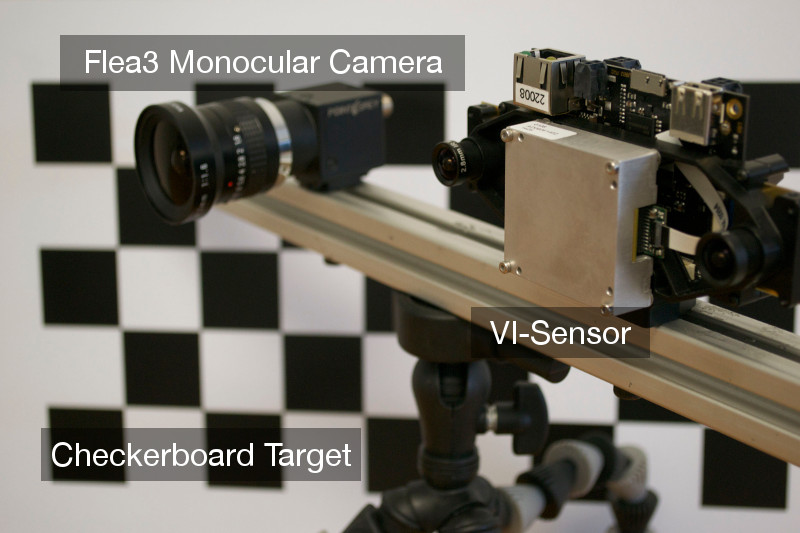
\includegraphics[width=0.4\textwidth]{probe/tricifix2}
    \caption{The Skybotix VI-Sensor, Point Grey Flea3, and checkerboard target used in our motion blur experiments.}
    \label{fig:probe_tricifix}
\end{figure}

%\begin{figure}
%    \centering
%    \includegraphics[width=0.4\textwidth]{figs/blurMetric_short}
%    \caption{Blur metric \cite{Anonymous:Ngi3VEEU} computed for the left camera of the VI-Sensor for the checkerboard dataset. We separate the dataset into regions of high and low blur corresponding to fast and slow motion, respectively.}
%    \label{fig:visensor_blurMetric}
%\end{figure}


\begin{figure}
    \centering
        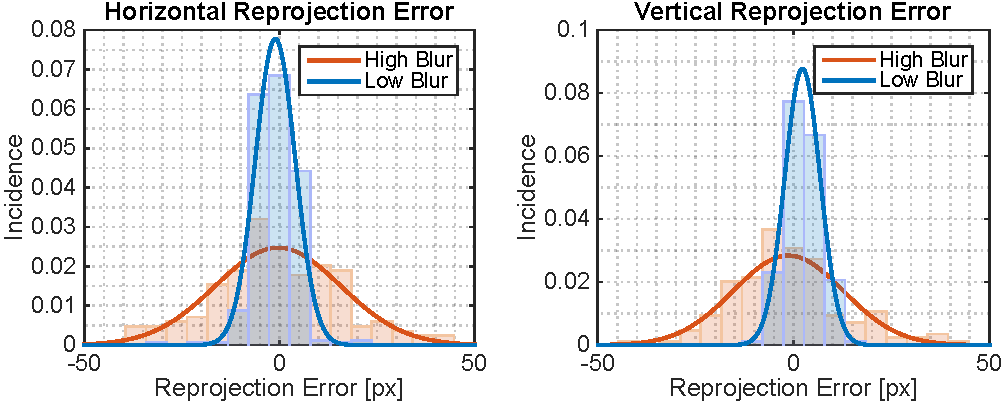
\includegraphics[width=0.85\textwidth]{probe/reprojectionError}
        \label{fig:probe_visensor_reprojectionError}
      \caption{Reprojection error of checkerboard corners triangulated from the VI-Sensor and reprojected into the Flea3.We distinguish between high and low blur by thresholding the blur metric \cite{crete2007blur}.}
\end{figure}

\begin{figure}
    \centering
    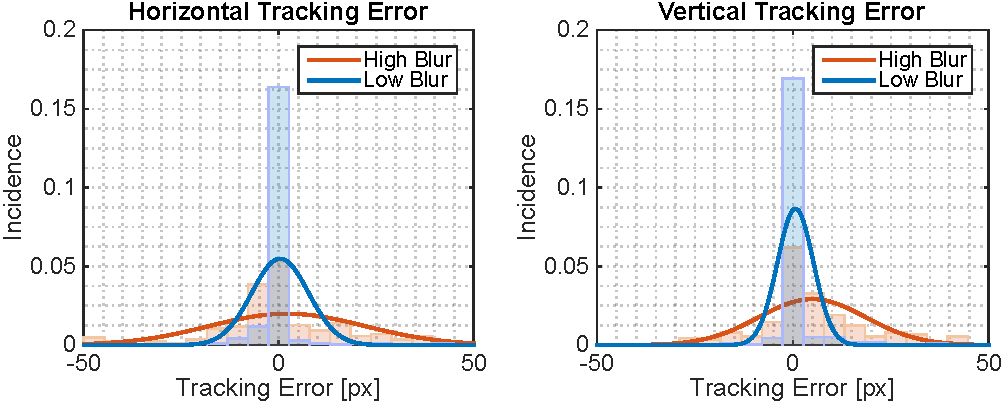
\includegraphics[width=0.85\textwidth]{probe/trackingError}
    \label{fig:probe_visensor_trackingError}
    \caption{Effect of blur on reprojection and tracking error for the slow-then-fast checkerboard dataset. We distinguish between high and low blur by thresholding the blur metric \cite{crete2007blur}. The variance in both errors increases with blur.}
    \label{fig:probe_visensor_histograms}
\end{figure}

We detected checkerboard corners in each camera at synchronized time steps, computed their 3D coordinates in the VI-Sensor frame, then reprojected these 3D coordinates into the Flea3 frame.
We then computed the reprojection error as the distance between the reprojected image coordinates and the true image coordinates in the Flea3 frame.
Since the Flea3 operated at a much higher frame rate than the VI-Sensor, it was less susceptible to motion blur and so we treated its observations as ground truth.
We also computed a tracking error by comparing the image coordinates of checkerboard corners in the left camera of the VI-Sensor computed from both KLT tracking \cite{Lucas:1981} and re-detection.

\Cref{fig:probe_visensor_histograms} shows histograms and fitted normal distributions for both reprojection error and tracking error.
From these distributions we can see that the errors remain approximately zero-mean, but that their variance increases with blur.
This result is compelling evidence that the effect of blur on feature tracking quality can be accounted for by scaling the feature covariance matrix by a function of the blur metric.


\subsection{Optical flow variance}
To detect moving objects, we compute a score for each feature based on the ratio of the variance in optical flow vectors in a small region around the feature to the variance in flow vectors of a larger region.
Intuitively, if the flow variance in the small region differs significantly from that in the larger region, we might expect the feature in question to belong to a moving object, and we would therefore like to trust the feature less.
Since we consider only the variance in optical flow vectors, we expect this predictor to be reasonably invariant to scene geometry.

We compute this optical flow variance score according to
\begin{equation}
    \log \left( \frac{\bar{\sigma}^2_s}{\bar{\sigma}^2_l} \right),
\end{equation}
where $\bar{\sigma}^2_s, \bar{\sigma}^2_l$ are the means of the variance of the vertical and horizontal optical flow vector components in the small and large regions respectively.
\Cref{fig:probe_flow_variance} shows sample results of this scoring procedure for two images in the KITTI dataset.
Our optical flow variance score generally picks out moving objects such as vehicles and cyclists in diverse scenes.

\begin{figure}
    \centering
    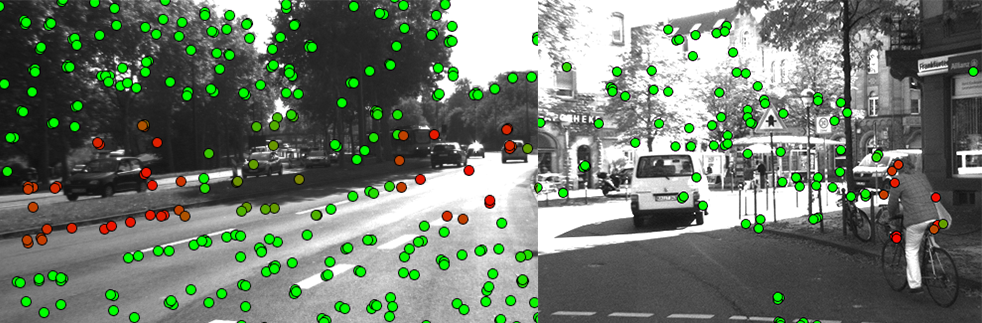
\includegraphics[width=0.8\textwidth]{probe/flowPredictorCombined.png}
    \caption{The optical flow variance predictor can help in detecting moving objects. Red circles correspond to higher values of the optical flow variance score (i.e., features more likely to belong to a moving object).}
    \label{fig:probe_flow_variance}
\end{figure}

\subsection{Image frequency composition}
Reliable feature tracking is often difficult in textureless or self-similar environments due to low feature counts and false matches.
We detect textureless and self-similar image regions by computing the Fast Fourier Transform (FFT) of each image and analyzing its frequency composition.
For each feature, we compute a coefficient for the low- and high-frequency regimes of the FFT.
\Cref{fig:probe_high_frequency} shows the result of the high-frequency version of this predictor on a sample image from the KITTI dataset.
Our high-frequency predictor effectively distinguishes between textureless regions (e.g., shadows and roads) and texture-rich regions (e.g., foliage).


\begin{figure}
    \centering
    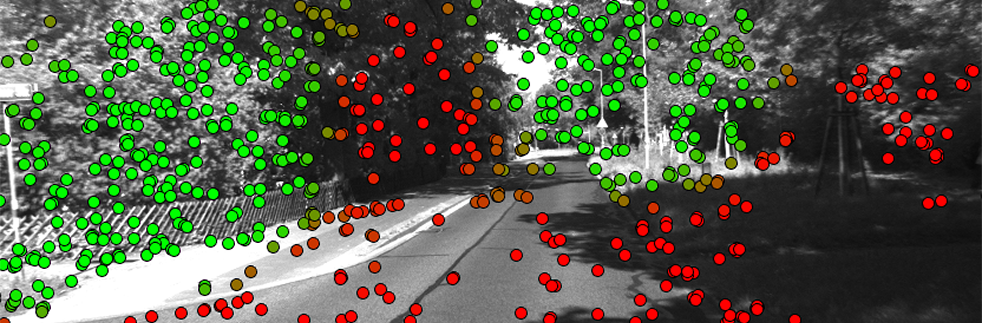
\includegraphics[width=0.8\textwidth]{probe/highFreqPredictor.png}
    \caption{A high-frequency predictor can distinguish between regions of high and low texture such as foliage and shadows. Green indicates higher values.}
    \label{fig:probe_high_frequency}
\end{figure}


\section{Experiments}
To validate PROBE-GK, we used three types of data: synthetic simulations, the
KITTI dataset, and our own experimental data collected at the University of
Toronto. 

\subsection{Simulation}
\subsubsection{Monte-Carlo Verification}
To begin, we verified that PROBE-GK can predict increasingly accurate estimates of the true error covariance as more training data is added. We developed a basic simulation environment consisting of a large amount of point landmarks being observed by a stereo camera. In our simulation, the camera traversed a single step in one direction, and recorded  empirical reprojection errors based on ground truth poses. We simulated additive Gaussian noise on image coordinates, and used Monte Carlo simulations (propagating the additive noise through \Cref{eq:image_error}) to estimate the true covariances. \Cref{fig:probe_frobNorm} shows the mean Frobenius norm (as defined in \cite{Barfoot2014-ac}) between the covariances estimated by PROBE-GK and the true covariances for a test trial. The mean norm tends to zero as more landmarks are added, indicating that PROBE-GK does learn the correct covariances.


\begin{figure}
    \centering
      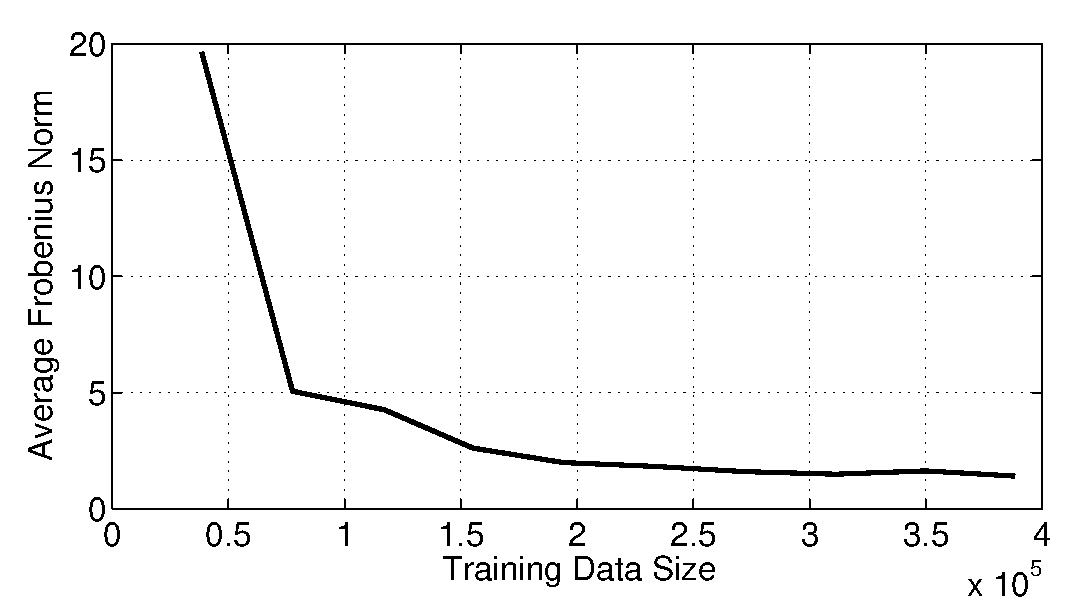
\includegraphics[width=0.45\textwidth]{probe-gk/frobNorm.eps}
     \caption{Mean Frobenius norm of the error between the estimated and true
       noise covariance as a function of training data size. The norm tends to
       zero as training data is added which indicates that PROBE-GK is learning
       the correct covariances.}
    \label{fig:probe_frobNorm}
\end{figure}


\subsubsection{Synthetic}

Next, we formulated a synthetic dataset wherein a stereo camera traverses a circular path observing 2000 randomly distributed point features.
We added Gaussian noise to each of the ideal projected
pixel co-ordinates for visible landmarks at every step. We varied the noise variance as a function of the vertical pixel coordinate of
the feature in image space. In addition, a small subset of the landmarks received an error term drawn from a uniform distribution to simulate the presence of outliers. The prediction space was composed of
the vertical and horizontal pixel locations in each of the stereo cameras.

\begin{figure}
\centering
   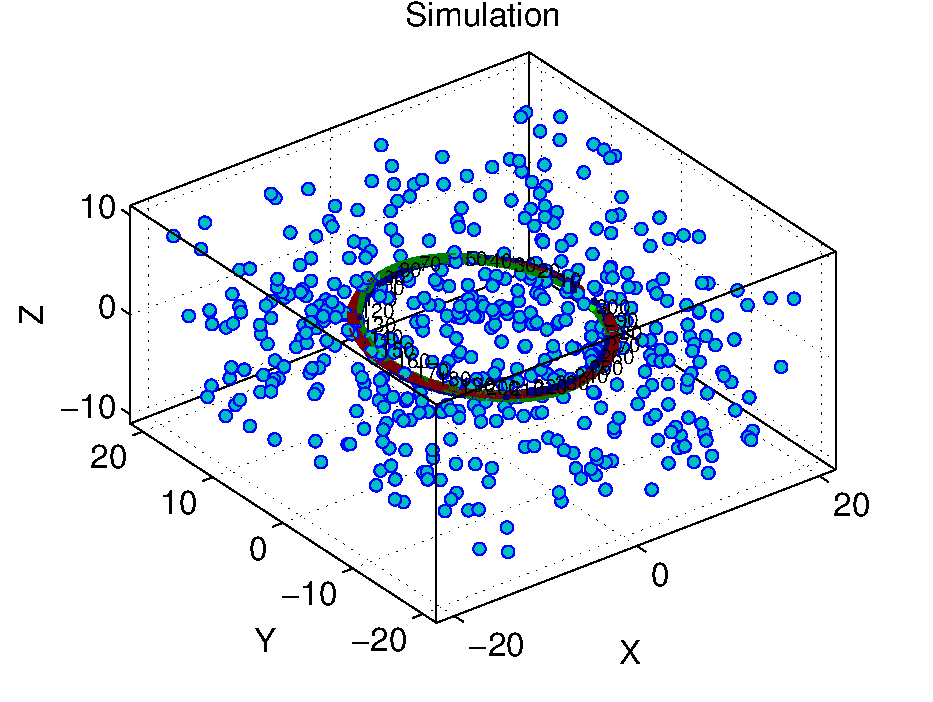
\includegraphics[width=0.5\textwidth]{probe-gk/sim_world.pdf}
   \label{fig:probe_SimWorld} 
\caption{Our synthetic world. A stereo camera rig moves through a world with 2000 point features.}
\end{figure}

We simulated independent training and test traversals, where the camera moved for
30 and 60 seconds respectively (at a forward speed of 3 metres per second for final path
lengths of 90 and 180 meters).  \Cref{fig:sim_comparison} and \Cref{table:probe-gk_armse_errors} document the qualitative and quantitative comparisons of PROBE-GK (trained with and without ground-truth) against two baseline stereo odometry frameworks. Both baseline estimators were implemented based on \Cref{sec:ssvo}. The first utilized fixed covariances for all reprojection errors, while the second used a modified robust cost (i.e. M-estimation) based on Student's~$t$ weighting, with $\nu = 5$ (as suggested in \cite{kerl2013robust}).  These benchmarks served as baseline estimators (with and without robust costs) that used fixed covariance matrices and did not include a predictive component. 

Using PROBE-GK with ground truth data for training,
we significantly reduced both the translation and rotational Average Root Mean Squared Error (ARMSE)
by approximately 50\%. In our synthetic data, the Expectation Maximization approach was able to achieve nearly identical results to the ground-truth-aided model within 5 iterations.  

\begin{figure}
    \centering
    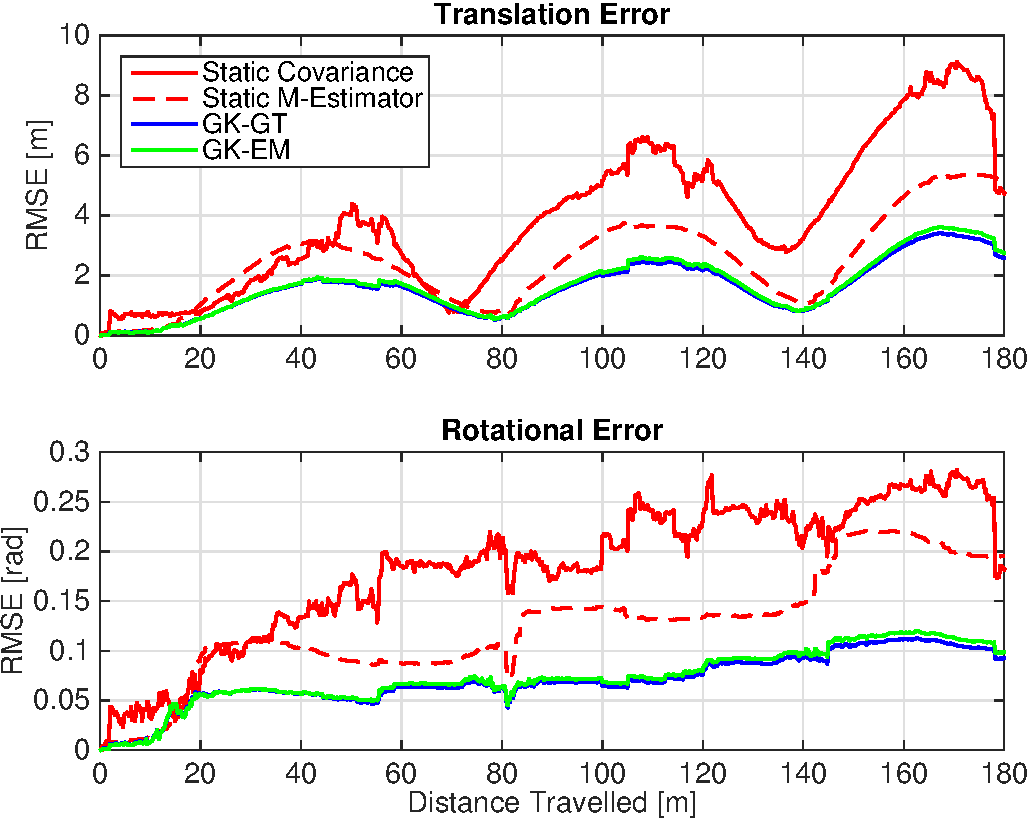
\includegraphics[width=0.75\textwidth]{probe-gk/simComparison_sim_rerun}
    \caption{A comparison of translational and rotational Root Mean Square Error on simulated data
    (RMSE) for four different stereo-visual odometry pipelines: two baseline
    bundle adjustment procedures with and without a robust Student's~$t$ cost with a fixed and
    hand-tuned covariance and degrees of freedom (M-Estimation), a robust bundle
    adjustment with covariances learned from ground truth with
    \cref{alg:train-ground-truth} (GK-GT), and a robust bundle adjustment using
    covariances learned without ground truth using expectation maximization,
    with \cref{alg:train-em} (GK-EM). Note in this experiment, the RMSE curves
    for GK-GT and GK-EM very nearly overlap. The overall translational and
    rotational ARMSE values are shown in Table \ref{table:probe-gk_armse_errors}.} 
    \label{fig:sim_comparison}
\end{figure}

\subsection{KITTI}

\begin{figure}
    \centering
    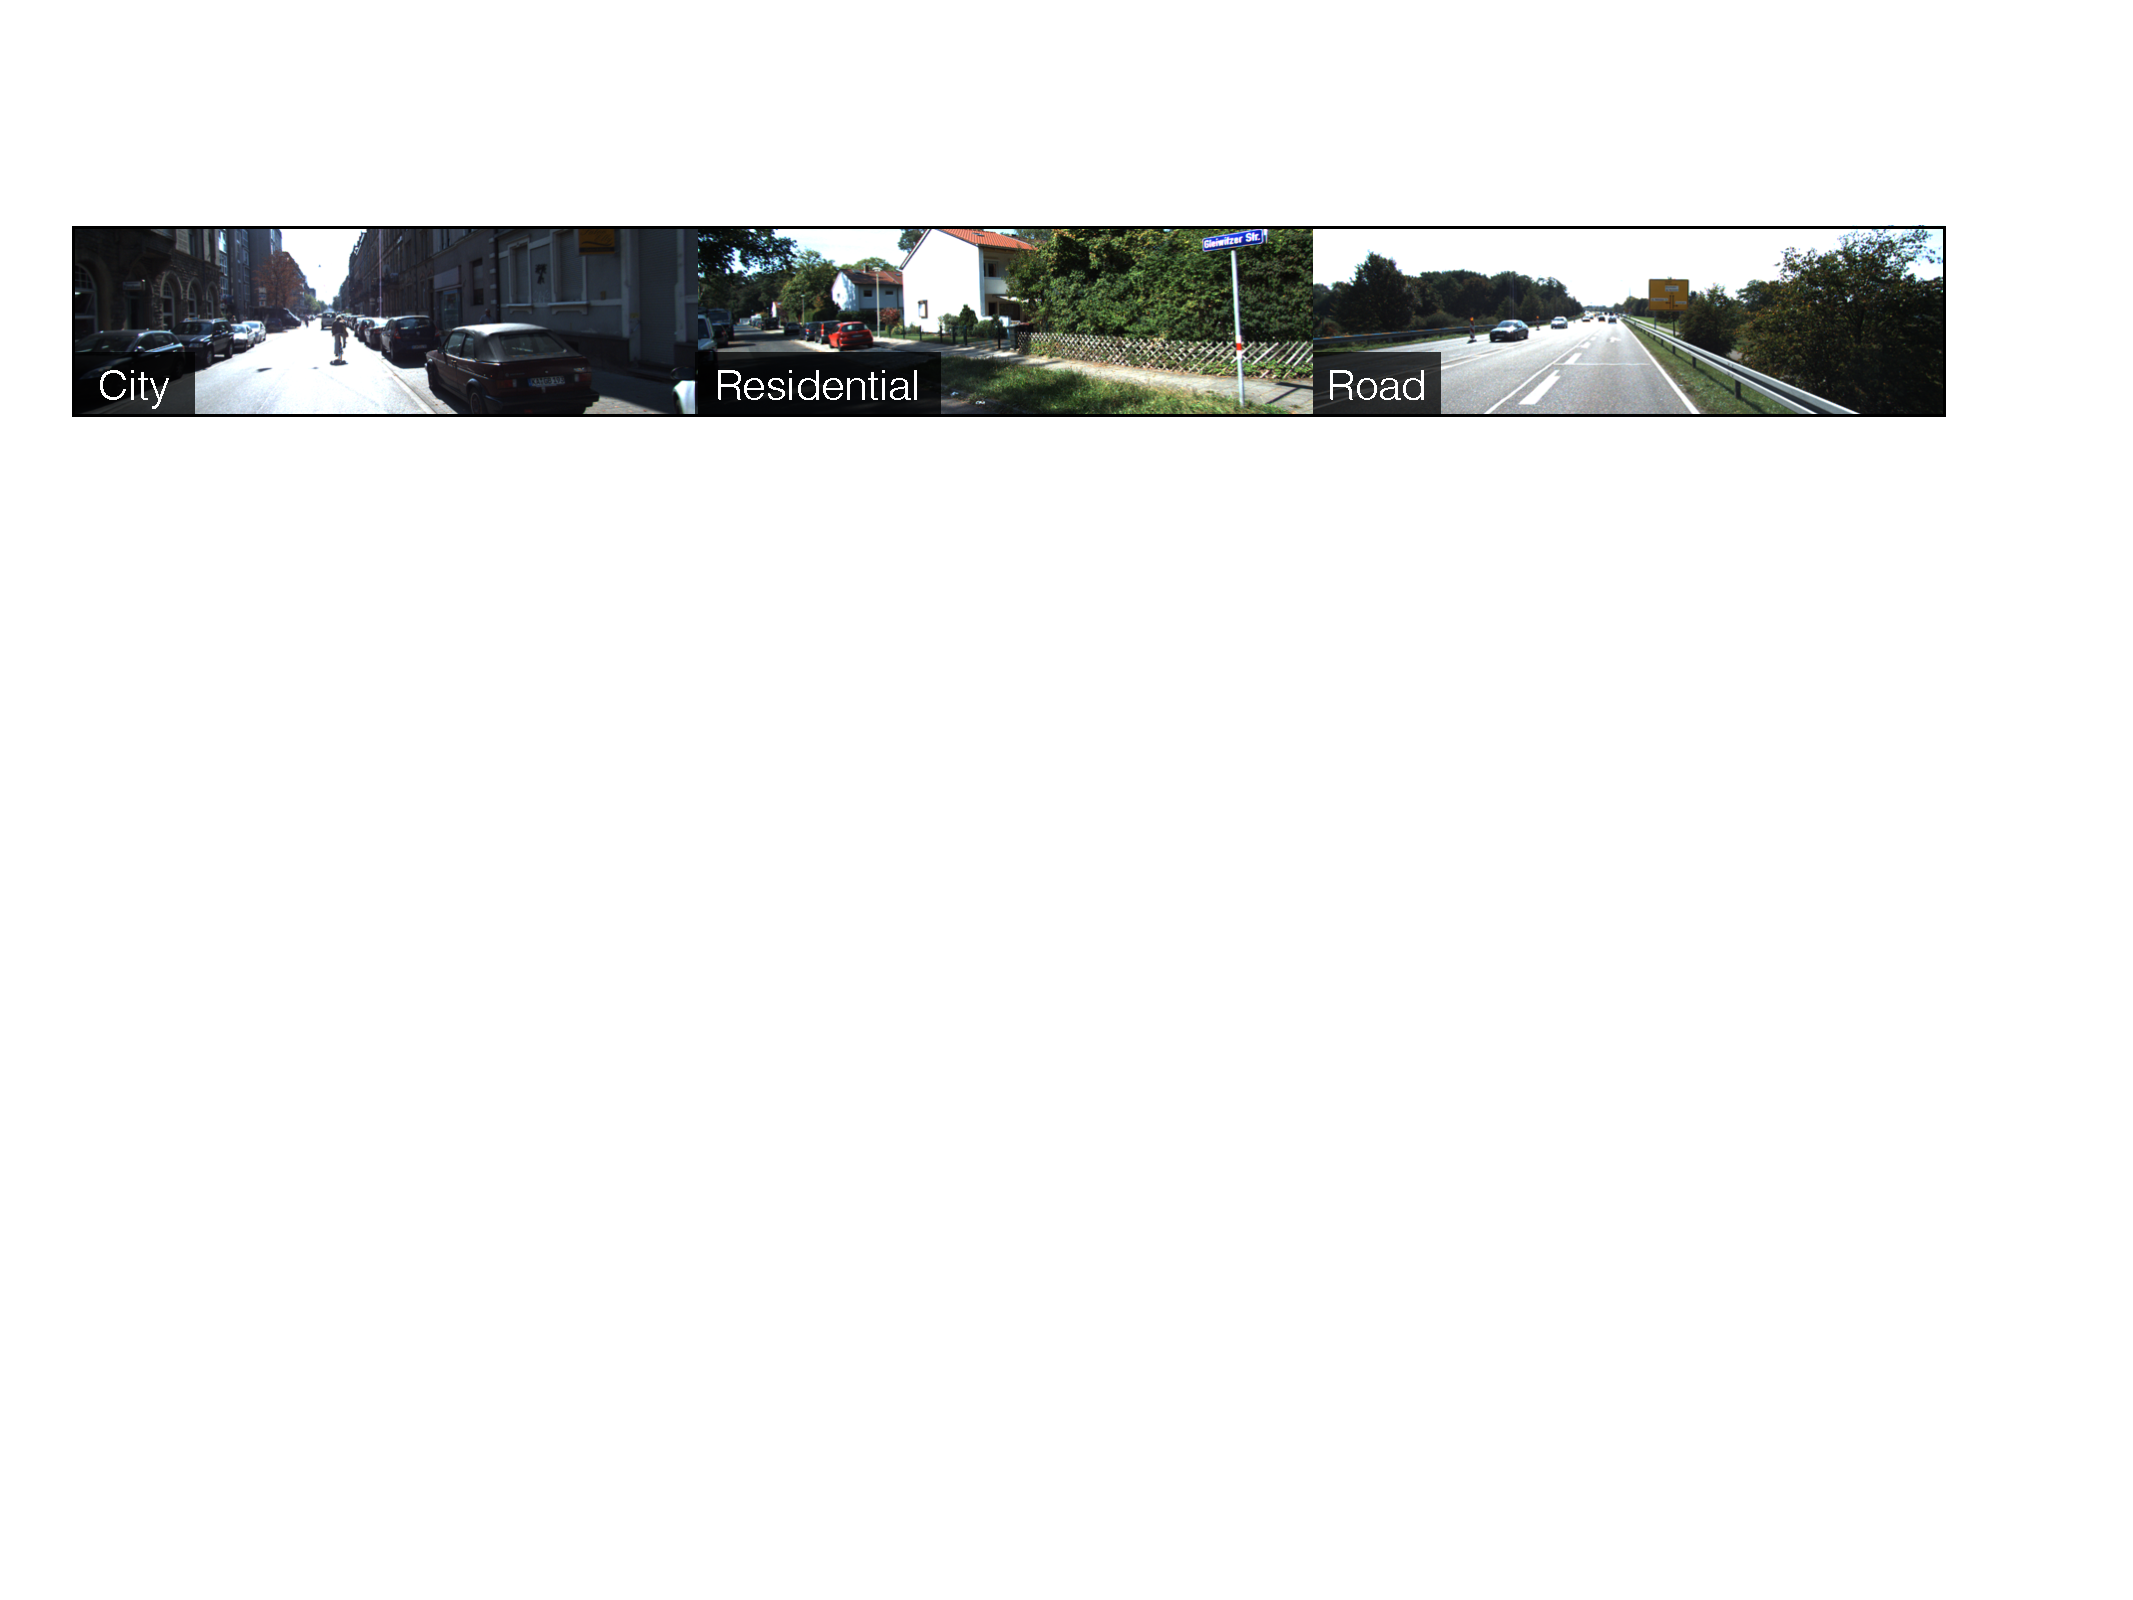
\includegraphics[width=0.98\textwidth]{probe-gk/KittiEnvironments}
    \caption{The KITTI dataset contains three different environments. We
      validate PROBE-GK by training on each type and testing against a baseline
      stereo visual odometry pipeline.}
      \vspace{-0.5em}
    \label{fig:kitti_environments}
\end{figure}

To evaluate PROBE-GK on real environments, we trained and tested several models on
the KITTI Vision Benchmark suite \citep{Geiger2013-ky}, a series of datasets collected by a car outfitted with a number of
sensors driven around different parts of Karlsruhe, Germany. Within the dataset, ground truth pose information is
provided by a high grade inertial navigation unit which also fuses measurements from differential GPS. Raw data
is available for different types of environments through which the car was driving; for our
work, we focused on the city, residential and road categories
(\Cref{fig:kitti_environments}).  From each category, we chose two separate trials for training and testing.

\begin{figure}
    \centering
    \includegraphics[width=0.75\textwidth]{probe-gk/{kittiComparison-0011-0009-15-Sep-2015-4way}}
    \caption{RMSE comparison of stereo odometry estimators evaluated on data from the city category in the KITTI dataset. See \Cref{table:probe-gk_armse_errors} for a quantitative summary.}
    \vspace{-0.4em}
    \label{fig:probe-gk_kitti_comparison1}
\end{figure}



\begin{figure}
    \centering
    \includegraphics[width=0.75\textwidth]{probe-gk/{kittiComparison-0035-0036-15-Sep-2015-4way}}
    \caption{RMSE comparison of stereo odometry estimators evaluated on data from the residential category in the KITTI dataset.}
    \vspace{-0.4em}
    \label{fig:probe-gk_kitti_comparison2}
\end{figure}

\begin{figure}
    \centering
    \includegraphics[width=0.75\textwidth]{probe-gk/{kittiComparison-0070-0028-15-Sep-2015-4way}}
    \caption{RMSE comparison of stereo odometry estimators evaluated on data from the road category in the KITTI dataset.}
    \vspace{-0.4em}
    \label{fig:probe-gk_kitti_comparison3}
\end{figure}

\Cref{fig:probe-gk_kitti_comparison1,fig:probe-gk_kitti_comparison2,fig:probe-gk_kitti_comparison3} show
typical results; \Cref{table:probe-gk_armse_errors} presents a quantitative comparison.
PROBE GK-GT produced significant reductions in ARMSE, reducing translational ARMSE by
as much as 80\%. In contrast, GK-EM showed more modest improvements; this is
unlike our synthetic experiments, where both GK-EM and GK-GT achieved similar
performance. We are still actively exploring why this is the case; we note that although our simulated
data is drawn from a mixture of Gaussian distributions, the underlying
noise distribution for real data may be far more complex. With no ground truth, EM has to jointly optimize the camera poses and sensor uncertainty. It is unclear whether this is feasible in the general case with no ground truth information.

Further, we observe that the performance of PROBE-GK depends on the similarity
of the training data to the final test trials. A characteristic training dataset was important for consistent improvements on test trials.


\subsection{UTIAS}

\begin{table}
\centering
\caption{Comparison of average root mean squared errors (ARMSE) for rotational
  and translational components. Each trial is trained and tested from a
  particular category of raw data from the synthetic and KITTI datasets.}

\resizebox{\columnwidth}{!}{%
\begin{tabular}{l c c c c c c c c c }
 & & \multicolumn{4}{c}{Trans. ARMSE [m]} & \multicolumn{4}{c}{Rot. ARMSE [rad]}  \\  \cline{3-6}  \cline{7-10} \T                                                                                    
 & Length [m] & Fixed Covar. & Static M-Estimator  & GK-GT & GK-EM & Fixed Covar. &  Static M-Estimator  & GK-GT & GK-EM  \\                         
\hline \T
Synthetic & 180 & 3.87 & 2.49 & 1.59 & 1.66 & 0.18 & 0.13 & 0.070 & 0.073 \\                                                                                                                
City & 332.9 & 3.84 & 2.99 & 1.69 & 2.87 & 0.032 & 0.021 & 0.0046 & 0.018 \\ 
Residential & 714.1 & 13.48 & 9.37 & 1.97 & 8.80 & 0.068 & 0.050 & 0.013 & 0.044 \\
Road & 723.8 & 17.69 & 9.38 & 5.24 & 8.87 & 0.060 & 0.027 & 0.015 & 0.024
\\ \hline                                                                                                                
\end{tabular}               \label{table:probe-gk_armse_errors}
}
\end{table}

\begin{figure}
    \centering
    \hspace*{0.25cm}
    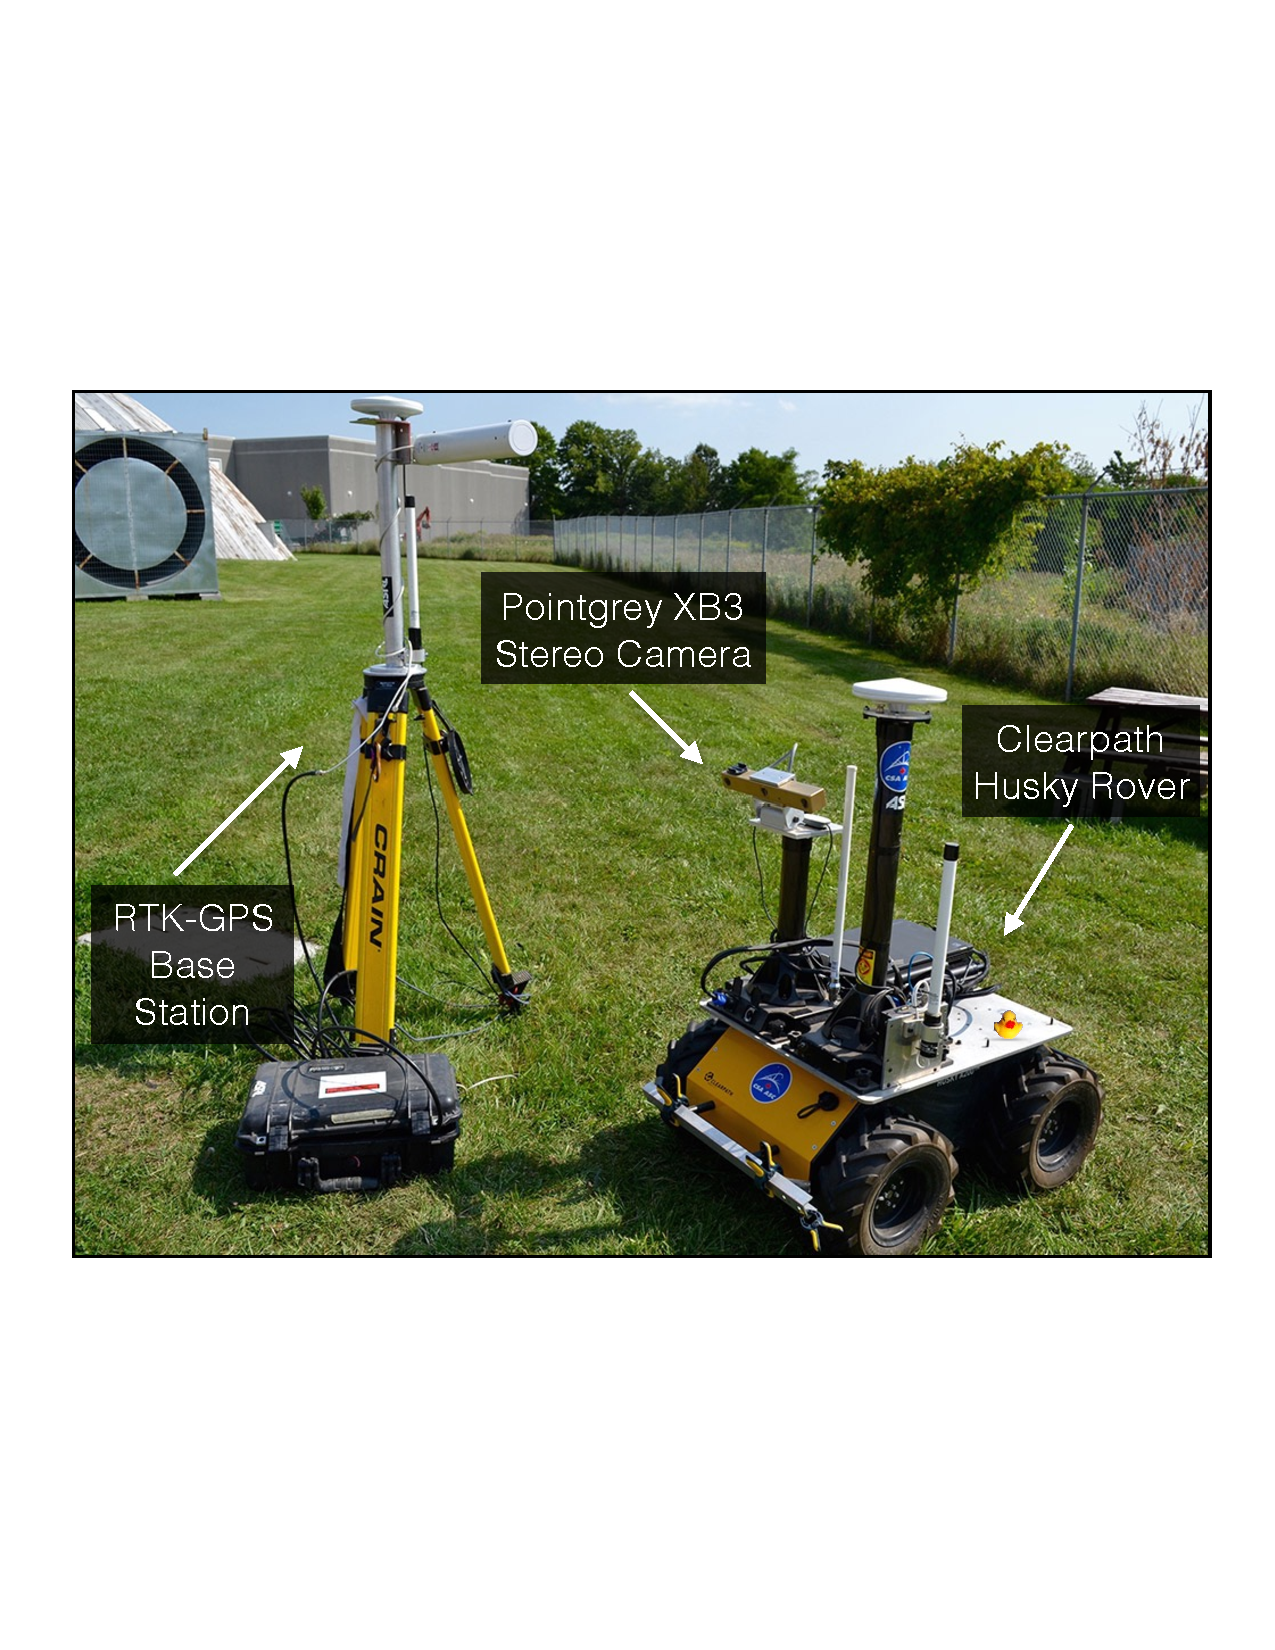
\includegraphics[width=0.75\textwidth]{probe-gk/experiment_wide_border}
    \caption{Our experimental apparatus: a Clearpath Husky rover outfitted with a PointGrey XB3 stereo camera and a differential GPS receiver and base station.}
      \vspace{-0.5em}
   	    \label{fig:probe-gk_experiments}
\end{figure}

\begin{figure}
    \centering
	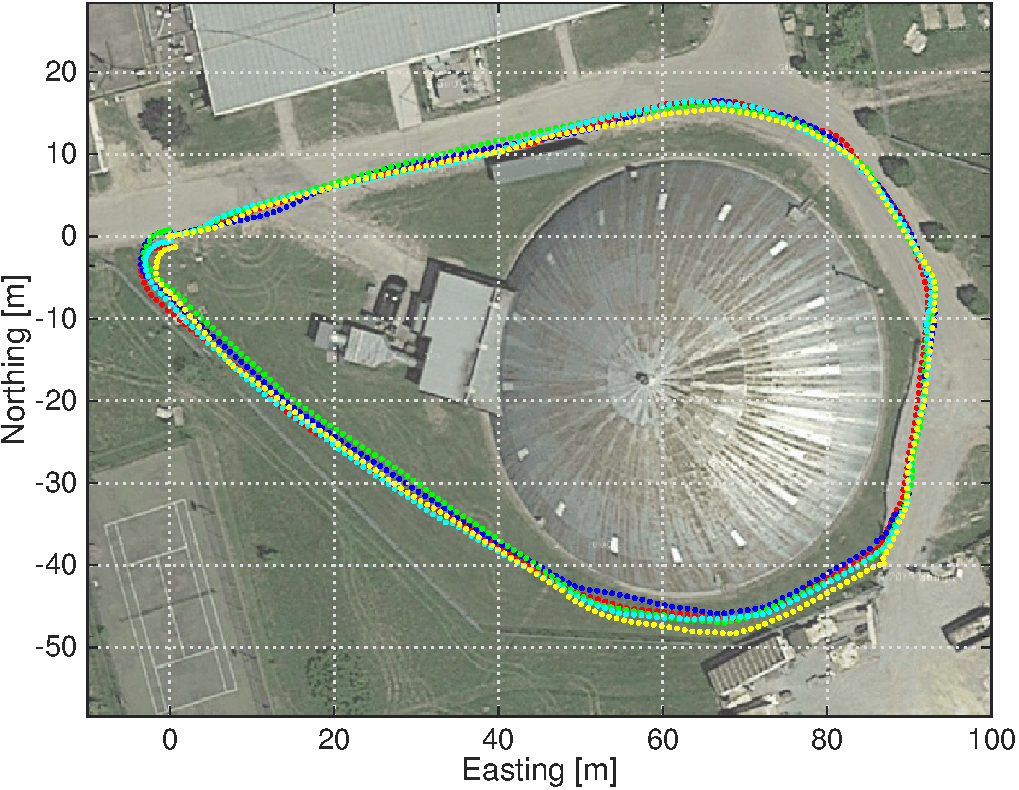
\includegraphics[width=0.75\textwidth]{probe-gk/xb3_rtk_fig}
    \caption{GPS ground truth for 5 experimental trials collected
      near the UTIAS Mars Dome. Each trial is approximately 250 m long.}
      \vspace{-0.5em}
    \label{fig:probe-gk_experiment_groundtruth}
\end{figure}

\begin{figure}
    \centering
    \includegraphics[width=0.75\textwidth]{probe-gk/{trainingStats}}
    \caption{Training without ground truth using PROBE-GK-EM on a 250.2m path
      around the Mars Dome at UTIAS. The likelihood of the data increases with
      each iteration, and the loop closure error decreases, improving significantly from a baseline static M-estimator.}
      \vspace{-1em}
    \label{fig:probe-gk_experiments_trainingstats}
\end{figure}


To further investigate the capability of our EM approach, we evaluated PROBE-GK on experimental data collected at the University of Toronto Institute for Aerospace Studies (UTIAS). For this experiment, we drove a Clearpath Husky rover outfitted with an Ashtech DG14 Differential GPS, and a PointGrey XB3 stereo camera around the MarsDome (an indoor Mars analog testing environment) at UTIAS (\Cref{fig:probe-gk_experiments}) for five trials of a similar path.  Each trial was approximately 250 m in length and we made an effort to align the start and end points of each loop. We used the wide baseline (25 cm) of the XB3 stereo camera to record the stereo images. The approximate trajectory for all 5 trials, as recorded by GPS, is shown in \Cref{fig:probe-gk_experiment_groundtruth}.  Note that the GPS data was not used during training, and only recorded for reference.

For the prediction space in our experiments, we mimicked the KITTI experiments, omitting inertial magnitudes as no inertial data was available. We trained PROBE-GK without ground truth, using the Expectation Maximization approach. \Cref{fig:probe-gk_experiments_trainingstats} shows the likelihood and loop closure error as a function of EM iteration. 

The EM approach indeed produced significant error reductions on the training dataset after just a few iterations.  Although  it was trained with no ground truth information, our PROBE-GK model was used to produce significant reductions in the loop closure errors of the remaining 4 test trials. This reinforced our earlier hypothesis: the EM method works well when the training trajectory more closely resembles the test trials (as was the case in this experiment). \Cref{table:probe-gk_loop_closure_errors} lists the statistics for each test. 


\begin{table}
\centering
\caption{Comparison of loop closure errors for 4 different experimental trials
  with and without a learned PROBE-GK-EM model.}
\begin{tabular}{ c  c  c  c }
     & & \multicolumn{2}{c}{Loop Closure Error [m]}  \\ \cline{3-4} \T
    Trial & Path Length [m] & PROBE-GK-EM & Static M-Estimator \\    
      \hline \T	
  2 & 250.3 & 3.88 & 8.07 \\
  3 & 250.5 & 3.07 & 6.64 \\
  4 & 205.4 & 2.81 & 7.57 \\
  5 & 249.9 & 2.34 & 7.75 \\ \hline
\end{tabular}
\label{table:probe-gk_loop_closure_errors}
\end{table}


\section{Summary}

Predictive Robust Estimation (PROBE) applied Generalized Kernel estimation to improve on the uncorrelated and static Gaussian error models typically employed in stereo odometry. By building a non-parametric predictive model for the density of reprojection errors, we derived a robust least squares objective whose parameters were predicted based on training data. In summary, this chapter contributed
\begin{enumerate}
\item a probabilistic model for indirect stereo visual odometry, leading to a predictive robust algorithm for inference on that model,
\item an efficient approach to constructing the robust algorithm based on Generalized Kernel (GK) estimation,
\item a procedure for training our model using pairs of stereo images with known relative transforms, and
\item an iterative, expectation-maximization approach to train our GK model when the relative ground truth egomotion was unavailable.
\end{enumerate}

%In this work, we presented PROBE, a novel method for predicting the quality of visual features within complex, dynamic environments. By using training data to learn a mapping from a predefined space of visual-inertial predictors to a scalar weight, we can adjust the influence of individual visual features on the final navigation estimate. PROBE can be used in place of traditional outlier rejection techniques such as RANSAC, or combined with them to more intelli- gently weight inlier measurements.
%We explored a variety of potential predictors, and validated our technique using a visual-inertial navigation system on over 4 km of data from the KITTI dataset and 700 m of indoor and outdoor data collected at the University of Toronto Institute for Aerospace Studies. Our results show that PROBE outperforms RANSAC-based binary outlier re- jection in many environments, even with only sparse ground truth available during the training step.
%In future work, we plan to examine a broader set of predic- tors, and extend the training procedure to incorporate online learning using intermittent ground truth measurements or loop closures detected by a place recognition thread. Further, we are interested in analyzing the amount of training data required for a given improvement in navigation accuracy, and in investigating PROBE’s effect on estimator consistency.


% By inferring a more accurate noise model given past sensory experience, we can reduce the tracking error of a sequence of estimates and improve the robustness of our estimator, even when the training data does not have associated ground truth. Our method has the advantage of having relatively few tuning parameters, meaning it can be applied to new problems with very little user intervention. We do rely on the availability of a good set of predictors, and have found that for problems of interest finding a good set is not difficult; a principled choice of an optimal set of predictors, however, remains an interesting open problem.
%Although our experiments demonstrate utility only in the context of sequential maximum likelihood estimation on stereo vision data, we believe the model presented here can be applied to a more general class of filter or factor- based estimation algorithms, as well as to a more general class of sensors. In future work, we plan to investigate the applicability of our method to problems of simultaneous localization and mapping, explore the possibility of learning the predictive model online (obviating the need for training data), and examine more principled approaches to selecting an informative prediction space.

\chapter{Learned Probabilistic Sun Sensor}
\epigraph{He stepped down, avoiding any long look at her as one avoids long looks at the sun, but seeing her as one sees the sun, without looking.}{Leo Tolstoy, \textit{Anna Karenina}}
\label{ch:sun-bcnn}

\section{Introduction}

Given that we can infer useful uncertainty information from images, is it possible to infer both uncertainty and some other geometric quantity that can aid in egomotion estimation? In this chapter, we present a pseudo-sensor that can do just that. Namely, we train a deep parametric model (a Bayesian Convolutional Neural Network) to act as a \textit{virtual sun sensor} that aims to reproduce the output of a dedicated sun sensor from a single RGB image.  This project was a collaboration with Lee Clement. While we both contributed to its formulation, Lee lead the integration of sun information into a visual odometry pipeline, while I designed and implemented the learning components.

\begin{figure*}[h!]
\centering
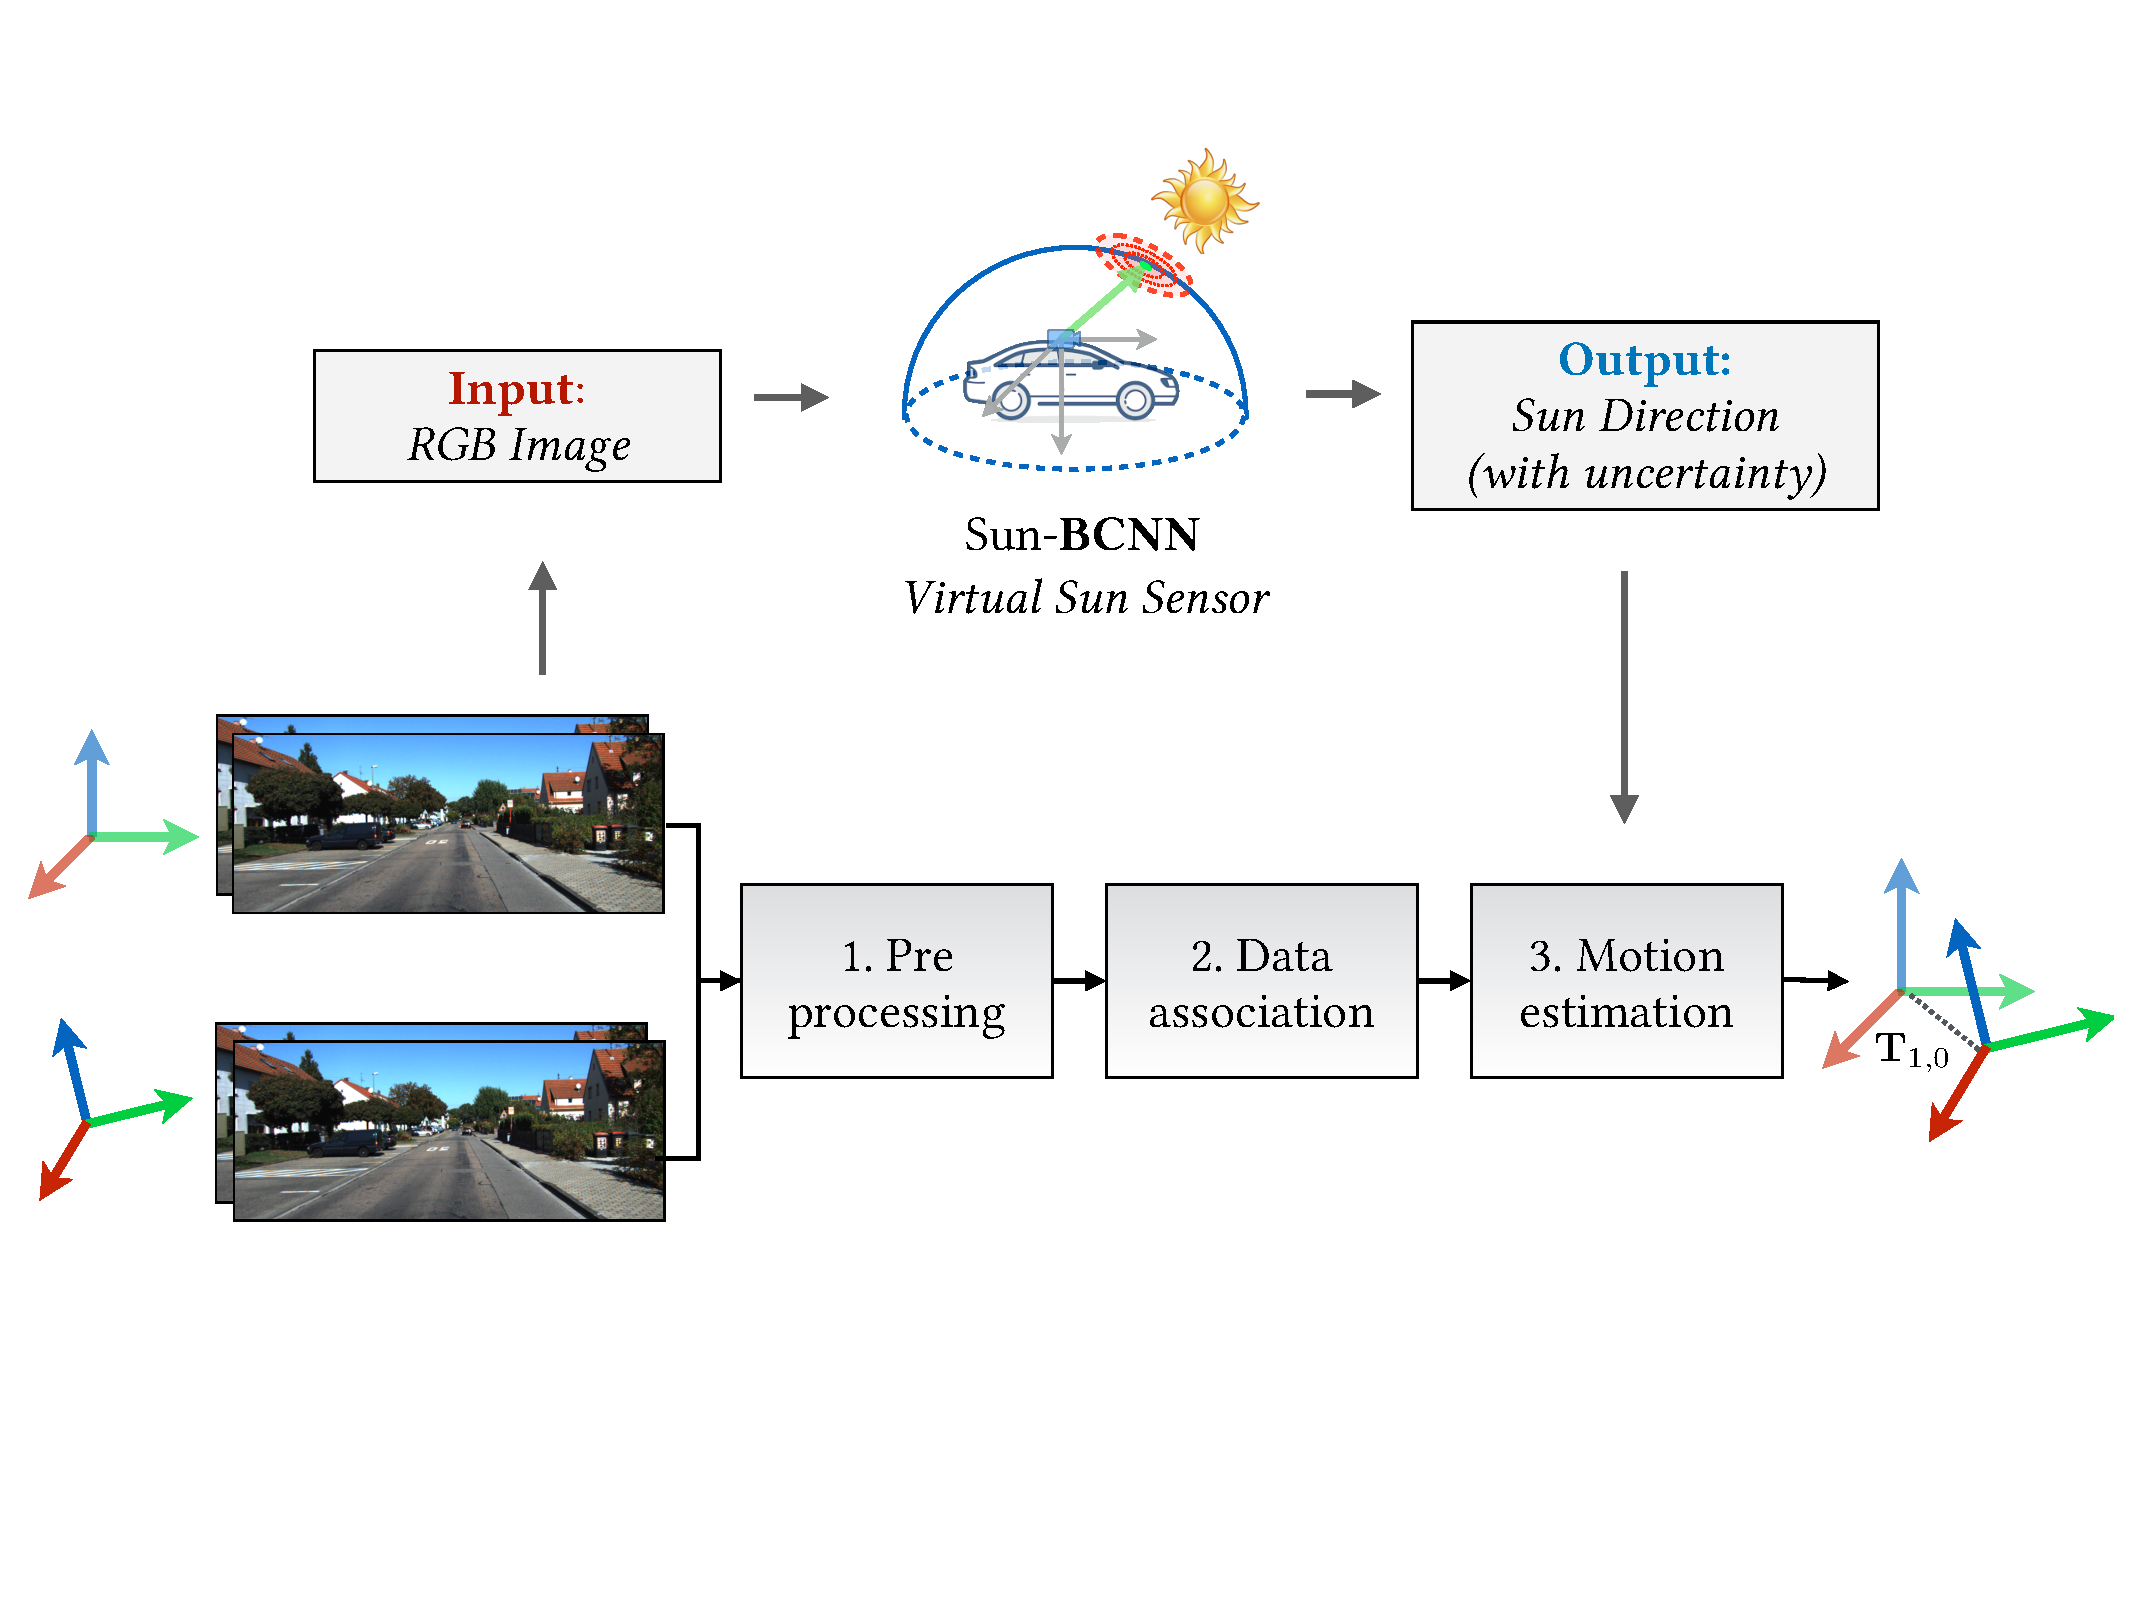
\includegraphics[width=0.8\textwidth]{sun-bcnn.pdf}
 \caption{Sun-BCNN is a learned virtual sun sensor that outputs sun direction with an associated uncertainty based on a single RGB image. We use this as a source of orientation information within a privileged reference frame.}
 \label{fig:sun-bcnn_intro_fig}
\end{figure*}

This work was associated with three publications:
\begin{enumerate}
\item \bibentry{2017_Clement_Improving},
\item \bibentry{2017_Peretroukhin_Reducing},
\item \bibentry{2018_Peretroukhin_Inferring}.
\end{enumerate}
This chapter is largely a reproduction of the latter journal publication which summarizes the approach.
 

\section{Motivation}
A crucial competency of any autonomous mobile robot is the ability to estimate its own motion through an operating environment.
While there exists a rich body of literature on the topic of motion estimation using a variety of techniques such as lidar-based point cloud matching \citep{Zhang2015} and visual-inertial odometry \citep{Leutenegger2015-fk}, egomotion estimation is fundamentally a process of dead-reckoning and will accumulate unbounded error over time.
This accumulated error, or drift, can be limited by incorporating global information into the motion estimation problem.
This frequently takes the form of a globally consistent map, loop closure detection, or reliance on additional sensors such as GPS to make corrections to the estimated trajectory.
In many situations, however, a globally consistent map may be unavailable or prohibitively expensive to compute, loop closures may not occur, or GPS may be unavailable or inaccurate.
In such cases, it can be advantageous to rely on environmental cues such as the sun, which can easily provide global orientation information since it is readily detectable and its apparent motion in the sky is well described by ephemeris models.


\begin{figure}
    \centering
    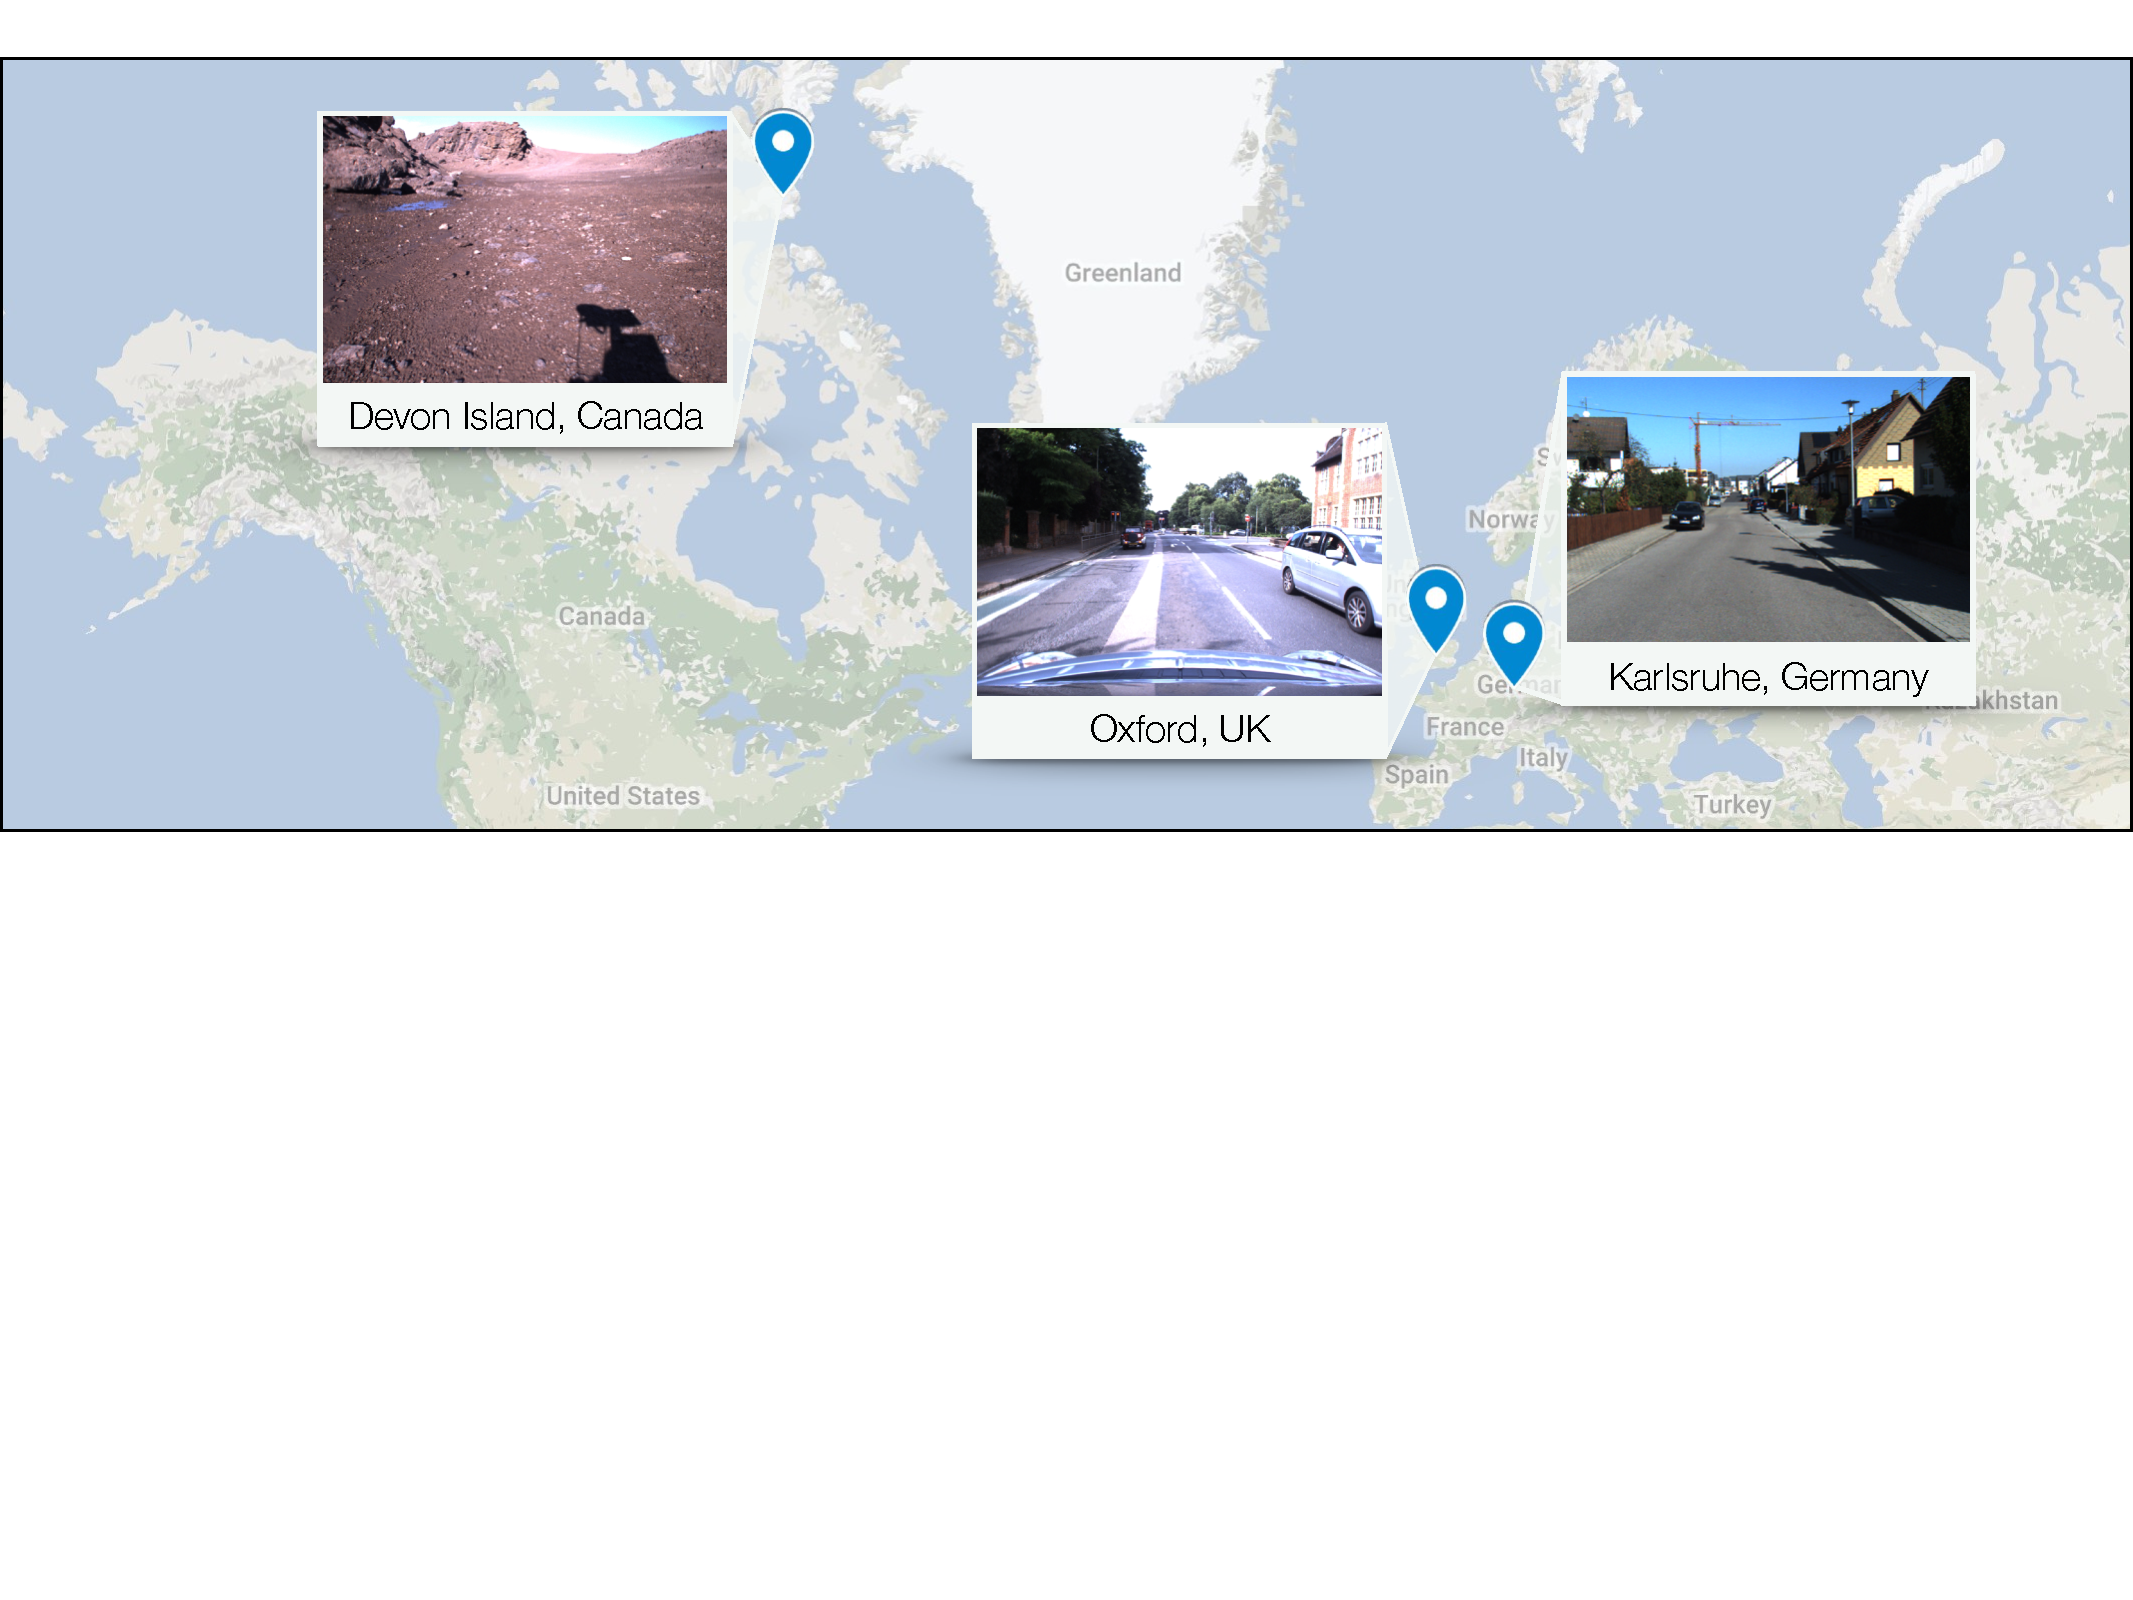
\includegraphics[width=0.98\textwidth]{sun-bcnn/all_datasets_gps}
    \caption{We train and test Sun-BCNN in a variety of environments ranging from urban driving in Europe to remote planetary analogue sites in the Canadian High Arctic. (Map data: Google, INEGI, ORION-ME.)}
    %\vspace{-0.4em}
    \label{fig:sun-bcnn_global-gps}
\end{figure}



\begin{wrapfigure}{r}{0.5\textwidth}
    \centering
      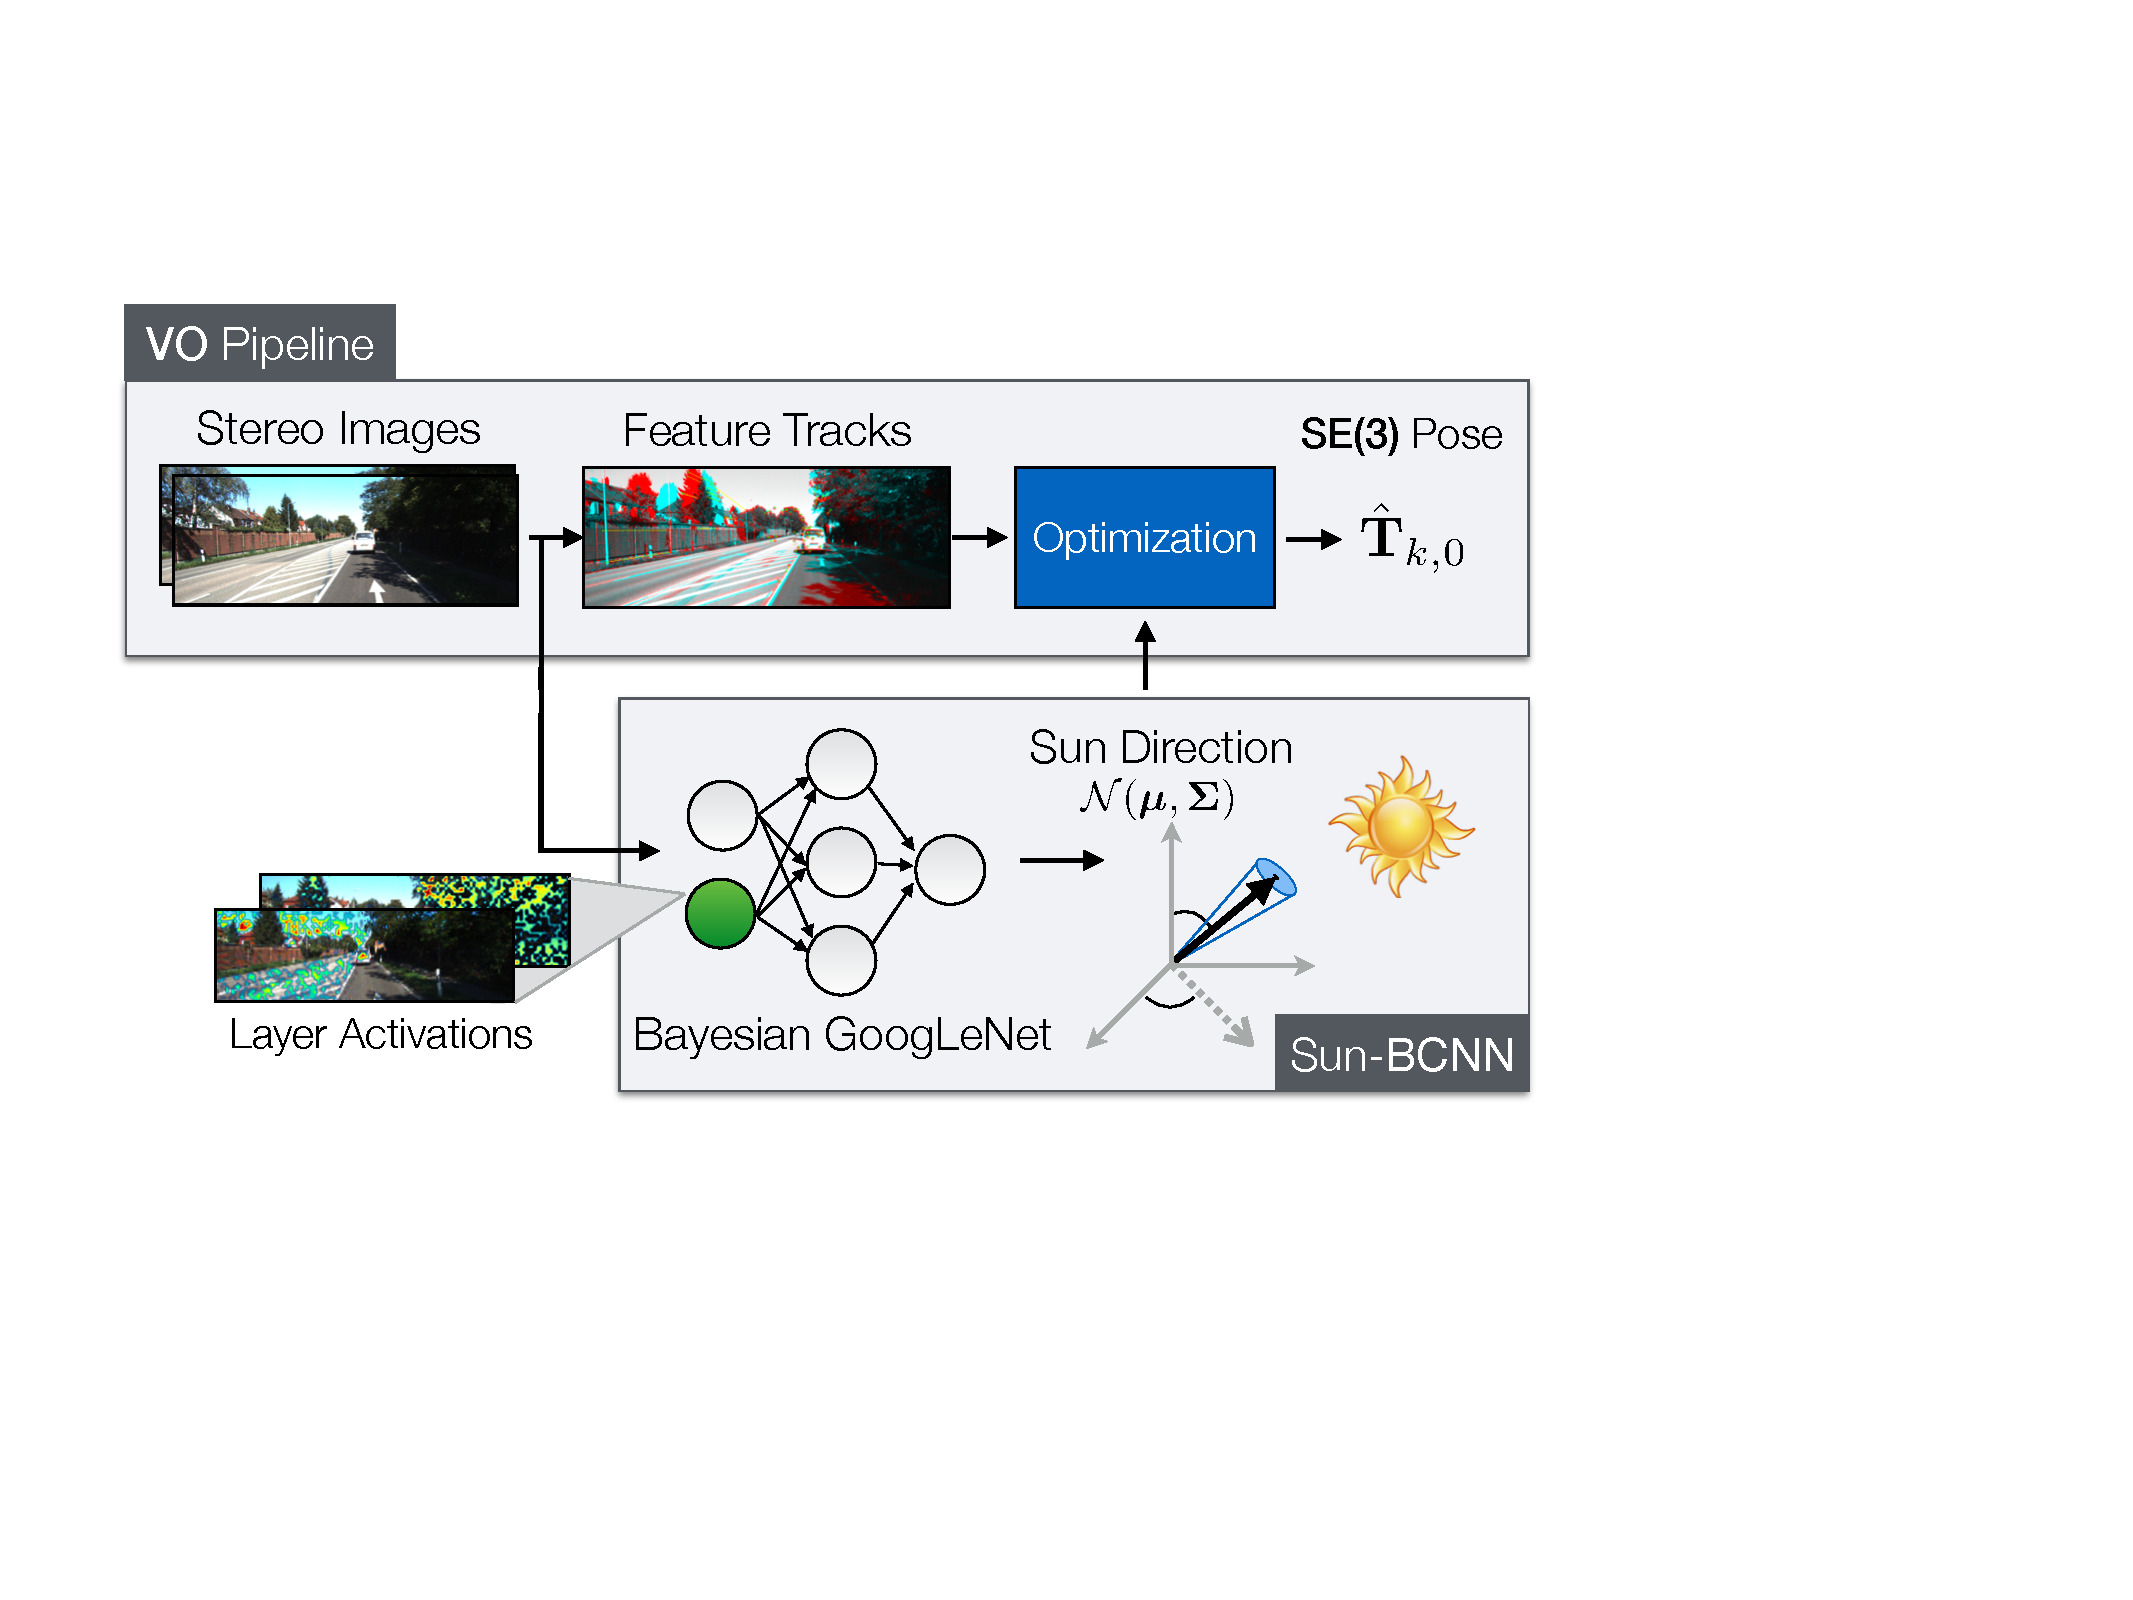
\includegraphics[width=0.48\columnwidth]{sun-bcnn/system_overview}
      \caption{Our method uses a Bayesian Convolutional Neural Network (BCNN) to estimate the direction of the sun and to produce a principled uncertainty estimate for each prediction. We incorporate this \emph{virtual sun sensor} into a stereo visual odometry pipeline to reduce estimation error.}
    \label{fig:sun-bcnn_system}
\end{wrapfigure}

For visual odometry (VO) in particular, the addition of global orientation information can limit the growth of drift error to be linear rather than superlinear with distance traveled \citep{Olson2003-ax}.

Sun-based orientation corrections have been successfully used in planetary analogue environments \citep{Furgale2011-zu,Lambert2012-sn} as well as on board the Mars Exploration Rovers (MERs) \citep{Eisenman2002-cg,Maimone2007-tc}.
In particular, \citet{Lambert2012-sn} showed that incorporating sun sensor and inclinometer measurements directly into the motion estimation pipeline (as opposed to periodically updating the vehicle heading, as in earlier work) can significantly reduce VO drift over long trajectories.


In this work, we seek to answer the question of whether similar reductions in VO drift can be obtained solely from the image stream already being used to compute VO.
The main idea here is that by reasoning over more than just the geometric information available from a standard RGB camera, we can improve existing VO techniques without needing to rely on a dedicated sun sensor or specially oriented camera.
In particular, we leverage recent advances in Bayesian Convolutional Neural Networks (BCNNs) to demonstrate how we can build and train a deep model capable of inferring the direction of the sun from a single RGB image. 
Moreover, we show that our network, dubbed Sun-BCNN, can produce a covariance estimate for each observation that obviates the need for a hand-tuned or empirically computed static covariance typically used for data fusion in a motion estimation pipeline. 




The remainder of this chapter begins with a discussion of related work, followed by an overview of the theory underlying BCNNs and a discussion of our model architecture, implementation, and training procedure.
We then outline our chosen visual odometry pipeline, which is based is an adapted version of the pipeline describe in \Cref{ch:vo}, and describe how observations of the sun can be incorporated directly into the motion estimation problem following the technique of \citet{Lambert2012-sn}.
Finally, we present several sets of experiments designed to test and validate both Sun-BCNN and our sun-aided VO pipeline in variety of environments.
These include experiments on 21.6~km of urban driving data from the KITTI odometry benchmark training set \citep{Geiger2013-ky}, as well as a further 10~km traverse through a planetary analogue site taken from the Devon Island Rover Navigation Dataset collected in a planetary analogue site in the Canadian High Arctic \citep{Furgale2012-kk}.
We investigate the possibility of model generalization between different cameras and environments, and further explore the sensitivity of Sun-BCNN to cloud cover during training and testing, using data from the Oxford Robotcar Dataset \citep{Maddern2016-ng}.
We also examine the impact of different methods for computing the mean and covariance of a norm-constrained vector on the accuracy and consistency of the estimated sun directions.

\section{Related Work}

Visual odometry (VO), a technique to estimate the motion of a moving platform equipped with one or more cameras, has a rich history of research including a notable implementation onboard the Mars Exploration Rovers (MERs) \citep{Scaramuzza2011-qr}. 
Modern approaches to VO can achieve estimation errors below 1\% of total distance traveled  \citep{Geiger2013-ky}. 
To achieve such accurate and robust estimates, modern techniques use careful visual feature pruning \citep{Cvisic2015-mt}, adaptive robust methods  \citep{Alcantarilla2016-kv,Peretroukhin2016-om}, or operate directly on pixel intensities \citep{Engel2015-il}.

Independent of the estimator, VO exhibits superlinear error growth, and is particularly sensitive to errors in orientation \citep{Olson2003-ax, Cvisic2015-mt}. 
One way to reduce orientation error is to incorporate observations of a landmark whose position or direction in the navigation frame is known \emph{a priori}. 
The sun is an example of such a known directional landmark. 
Accordingly, hardware sun sensors have been used to improve the accuracy of VO in planetary analogue environments (e.g., the Sinclair Interplanetary SS-411 sun sensor used by \citet{Furgale2011-zu} and \citet{Lambert2012-sn}), while the MERs articulated their Pancam apparatus to directly image the sun~\citep{Maimone2007-tc,Eisenman2002-cg}. 
More recently, software-based alternatives have been developed that can estimate the direction of the sun from a single image, making sun-aided navigation possible without additional sensors or a specially-oriented camera \citep{2017_Clement_Improving}. 
Some of these methods have been based on hand-crafted illumination cues such as shadows and variation in sky brightness \citep{Lalonde2011-jw,2017_Clement_Improving}, while others have attempted to learn such cues from data using deep Convolutional Neural Networks (CNNs) \citep{Ma2016-at}.

Convolutional Neural Networks (CNNs) have been applied to a wide range of classification, segmentation, and learning tasks in computer vision \citep{LeCun2015-qf}. 
Recent work has shown that CNNs can learn orientation information directly from images by modifying the loss functions of existing discrete classification-based CNN architectures into continuous regression losses \citep{Ma2016-at, Kendall2015-ew, Kendall2016-zf}. 
Despite their success in improving prediction accuracy, most existing CNN-based models do not report uncertainty estimates, which are important in the context of data fusion.

For classification, it is possible to restrict CNN model outputs to a certain range (e.g., using a softmax function) and interpret these values as the model's confidence in its output. As \citet{Gal2016UncertaintyThesis} noted, however, this can be misleading because these  values can be unjustifiably large for test points far away from training data.  To address this, \citet{Gal2016-ny} showed that it is possible to achieve covariance outputs that better quantify model uncertainty for classification and regression tasks, with only minor modifications to existing CNN architectures. 
An early application of this uncertainty quantification was presented by \citet{Kendall2016-zf} who used it to improve their prior work \citep{Kendall2015-ew} on camera pose regression.

We build on on previous work by \citet{2017_Clement_Improving}, who demonstrated empirically that techniques for single-image sun estimation based on hand-crafted models \citep{Lalonde2011-jw} and Convolutional Neural Networks (CNNs) \citep{Ma2016-at} could be incorporated into a stereo visual odometry pipeline to reduce estimation error in the manner of \citet{Lambert2012-sn}.
We also build on the work of \citet{2017_Peretroukhin_Reducing}, who presented preliminary experimental results comparing Sun-BCNN against the method of \citet{Lalonde2011-jw} and its VO-informed variant \citep{2017_Clement_Improving} as well as the Sun-CNN of \citet{Ma2016-at} on the KITTI odometry benchmark \citep{Geiger2013-ky}, both in terms of raw measurement accuracy and in terms of their impact on VO accuracy.

While our method is similar in spirit to the work of \citet{Ma2016-at}, who built a CNN-based sun sensor as part of a relocalization pipeline, our model makes three important improvements: 1) in addition to a point estimate of the sun direction, we output a principled covariance estimate that is incorporated into our estimator; 2) we produce a full 3D sun direction estimate with azimuth and zenith angles that is better suited to 6-DOF robot pose estimation problems (as opposed to only the azimuth angle and 3-DOF estimator used by \citet{Ma2016-at}); and 3) we incorporate the sun direction covariance into a VO estimator that accounts for growth in pose uncertainty over time (unlike \citet{2017_Clement_Improving}). 
Furthermore, our Bayesian CNN includes a dropout layer after every convolutional and fully connected layer (as outlined by \citet{Gal2016-ny} but not done by \citet{Kendall2016-zf}).

\section{Background}
\subsection{Neural Networks for Parametric Learning}


\subsection{Convolutional Neural Networks}
\subsection{Regularization and Dropout}

\begin{figure}
\centering
\begin{subfigure}{0.45\textwidth}
	\centering
    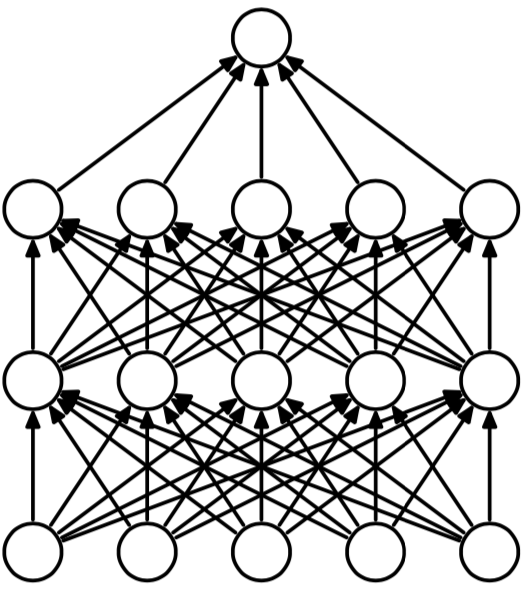
\includegraphics[width=0.8\textwidth]{sun-bcnn/dropout_fcn}
    \caption{Standard fully-connected neural network.}
\end{subfigure}
~
\begin{subfigure}{0.45\textwidth}
	\centering
    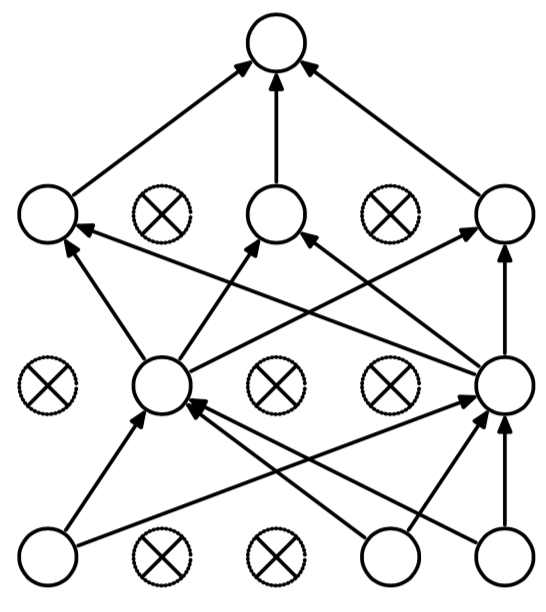
\includegraphics[width=0.8\textwidth]{sun-bcnn/dropout_fcnwdrop}
    \caption{A neural network with dropout applied.}
\end{subfigure}
\caption{The technique of \textit{dropout} stochastically removes the contribution of certain neurons to regularize learning. Figures	 from \cite{srivastava_dropout_2014}.}
\label{fig:sun-bcnn_dropout}
\end{figure}



\subsection{Dropout as Variational Inference}
\begin{align}
\label{eq:sun_direction_mean}
\Expectation{\Optimal{\Estimate{\SunDirection}}}_k &= \Optimal{\Estimate{\Mean{\SunDirection}}}_k \approx \frac{1}{N} \sum_{n=1}^N \Optimal{\Estimate{\SunDirection}}_k (\Optimal{\SunImage}_k, \CNNVariationalWeight^n) \\
\Expectation{\Optimal{\Estimate{\SunDirection}_k} \Transpose{\Optimal{\Estimate{\SunDirection}}}_k} &\approx \tau^{-1} \IdentityMatrix 
 +  \frac{1}{N} \sum_{n=1}^N \Optimal{\Estimate{\SunDirection}}_k(\Optimal{\SunImage}_k, \CNNVariationalWeight^n) \Transpose{\Optimal{\Estimate{\SunDirection}_k}(\Optimal{\SunImage}_k, \CNNVariationalWeight^n)} \notag \\ 
 &- \Optimal{\Estimate{\Mean{\SunDirection}}}_k \Transpose{\Optimal{\Estimate{\Mean{\SunDirection}}}_k},
 \label{eq:bcnn_covar}
\end{align}



\section{Sun-Aided Stereo Visual Odometry} 
\label{sec:sun_bcnn-stereo-vo}
We adopt a sliding window sparse stereo VO technique (adopted based on the frame-to-frame pipeline described in \Cref{ch:vo}) that has been used in a number of successful mobile robotics applications \citep{Cheng2006-nl,Furgale2010-to,Geiger2011-xe,Kelly2008-mh}.
Our task is to estimate a window of $\LieGroupSE{3}$ poses $\Set{\Transform_{k_1,0}, \Transform_{k_1+1,0}, \dots, \Transform_{k_2-1, 0}, \Transform_{k_2, 0}}$ expressed in a base coordinate frame $\CoordinateFrame{0}$, given a prior estimate of the transformation $\Transform_{k_1,0}$.
We accomplish this by tracking keypoints across pairs of stereo images and computing an initial guess for each pose in the window using frame-to-frame point cloud alignment, which we then refine by solving a local bundle adjustment problem over the window.
In our experiments we choose a window size of two, which we observed to provide good VO accuracy at low computational cost. 
We select the initial pose $\Transform_{1,0}$ to be the first GPS ground truth pose such that $\CoordinateFrame{0}$ is a local East-North-Up (ENU) coordinate system with its origin at the first GPS position.

\subsection{Observation Model}
We assume that incoming stereo images have been undistorted and rectified in a pre-processing step, and model the stereo camera as a pair of perfect pinhole cameras with focal lengths $f_u, f_v$ and principal points $\left(c_u,c_v\right)$, separated by a fixed and known baseline $b$ (see \Cref{sec:vo_data_extraction}).

If we take $\Keypoint_0^j$ to be the homogeneous 3D coordinates of keypoint $j$, expressed in our chosen base frame $\CoordinateFrame{0}$, we can transform the keypoint into the camera frame at pose $k$ to obtain $\Keypoint_k^j = \Transform_{k,0}\Keypoint_0^j = \Transpose{\bbm \KeypointComponent_{k,x}^j & \KeypointComponent_{k,y}^j & \KeypointComponent_{k,z}^j & 1 \ebm}$. Our observation model $\Vector{g}\left(\cdot\right)$ (defined with disparity, unlike the function $\Vector{f}(\cdot)$ in \Cref{sec:vo_data_extraction}) can then be formulated as
\begin{align} \label{eq:cam_model}
    \Vector{y}_{k,j} &= \CameraModel{\Keypoint_k^j}
%                    = \CameraModel{\Transform_{k,0} \Keypoint_0^j}
                    = \bbm u \\ v \T \\ d \T \ebm 
                    = \bbm 
			   		    f_u \KeypointComponent_{k,x}^j / \KeypointComponent_{k,z}^j + c_u \\
			   		    f_v \KeypointComponent_{k,y}^j / \KeypointComponent_{k,z}^j + c_v \T \\
			   		    f_u b / \KeypointComponent_{k,z}^j  \T
			         \ebm,
\end{align}
where $\left(u,v\right)$ are the keypoint coordinates in the left image and $d$ is the disparity in pixels.

\subsection{Sliding Window Bundle Adjustment}
Like with PROBE, we use the open-source \texttt{viso2} package \citep{Geiger2011-xe} to detect and track keypoints between stereo image pairs.
Based on these keypoint tracks, a three-point Random Sample Consensus (RANSAC) algorithm \citep{fischler1981random} generates an initial guess of the interframe motion and rejects outlier keypoint tracks by thresholding their reprojection error.
We compound these pose-to-pose transformation estimates through our chosen window and refine them using a local bundle adjustment, which we solve using the nonlinear least-squares solver Ceres \citep{ceres-solver}.
The objective function to be minimized can be written as
\begin{equation} \label{eq:cost_function}
    \BACost = \BACost_\text{reprojection} + \BACost_\text{prior},
\end{equation}
where
\begin{equation} \label{eq:reprojection_cost}
	\BACost_\text{reprojection} = \sum_{k=k_1}^{k_2} \sum_{j=1}^J \Transpose{\Error}_{\CameraObservation_{k,j}} \Covariance^{-1}_{\CameraObservation_{k,j}} \Error_{\CameraObservation_{k,j}}
\end{equation}
and 
\begin{equation} \label{eq:prior_cost}
	\BACost_\text{prior} = \Transpose{\Error}_{\Estimate{\Transform}_{k_1,0}} \Covariance^{-1}_{\Estimate{\Transform}_{k_1,0}} \Error_{\Estimate{\Transform}_{k_1,0}}.
\end{equation}

The quantity $\Error_{\CameraObservation_{k,j}} = \Estimate{\CameraObservation}_{k,j} - \CameraObservation_{k,j}$ represents the reprojection error of keypoint $j$ for camera pose $k$, with $\Covariance_{\CameraObservation_{k,j}}$ being the covariance of these errors.
The predicted measurements are given by $\Estimate{\CameraObservation}_{k,j} = \CameraModel{\Estimate{\Transform}_{k,0} \Estimate{\Keypoint}^j_{0}}$, where $\Estimate{\Transform}_{k,0}$ and $\Estimate{\Keypoint}^j_{0}$ are the estimated poses and keypoint positions in base frame $\CoordinateFrame{0}$.

The cost term $\BACost_\text{prior}$ imposes a normally distributed prior $\Prior{\Transform}_{k_1,0}$ on the first pose in the current window, based on the estimate of this pose in the previous window.
The error in the current estimate $\Estimate{\Transform}_{k_1,0}$ of this pose compared to the prior can be computed via the $\LieGroupSE{3}$ matrix logarithm as $\Error_{\Prior{\Transform}_{k_1,0}} = \log \left( \Prior{\Transform}_{k_1,0}^{-1} \Estimate{\Transform}_{k_1,0} \right)^\vee \in \mathbb{R}^6$.
The $6 \times 6$ matrix $\Covariance_{\Prior{\Transform}_{k_1,0}}$ is the covariance associated with $\Prior{\Transform}_{k_1,0}$ in its local tangent space, and is obtained as part of the previous window's bundle adjustment solution.
This prior term allows consecutive windows of pose estimates to be combined in a principled way that appropriately propagates global pose uncertainty from window to window, which is essential in the context of optimal data fusion.

\section{Orientation Correction}
In order to combat drift in the VO estimate produced by accumulated orientation error, we adopt the technique of \citet{Lambert2012-sn} to incorporate absolute orientation information from the sun directly into the estimation problem.
We assume the initial camera pose and its timestamp are available from GPS and use them to determine the global direction of the sun $\Vector{s}_0$, expressed as a 3D unit vector, from ephemeris data.
We define the world frame $\CoordinateFrame{0}$ to be a local ENU coordinate system with the initial GPS position as its origin.
At each timestep we update $\SunDirection_0$ by querying the ephemeris model using the current timestamp and the initial camera pose, allowing our model to account for the apparent motion of the sun over long trajectories.

By transforming the global sun direction into each camera frame $\CoordinateFrame{k}$ in the window, we obtain predicted sun directions $\Estimate{\SunDirection}_k = \Estimate{\Transform}_{k,0} \SunDirection_0$, where $\Estimate{\Transform}_{k,0}$ is the current estimate of camera pose $k$ in the base frame. 
We compare the predicted and estimated sun directions to introduce an additional error term into the bundle adjustment cost function (cf. \Cref{eq:cost_function}):
\begin{equation} \label{eq:cost_function_with_sun}
    \BACost = \BACost_\text{reprojection} + \BACost_\text{prior} + \BACost_\text{sun},
\end{equation}
where 
\begin{equation} \label{eq:sun_cost}
	\BACost_\text{sun} = \sum_{k=k_1}^{k_2} \Transpose{\Error}_{\SunDirection_k} \Covariance^{-1}_{\SunDirection_k} \Error_{\SunDirection_k},
\end{equation}
and $\BACost_\text{reprojection}$ and $\BACost_\text{prior}$ are defined in \Cref{eq:reprojection_cost,eq:prior_cost}, respectively.
This additional term constrains the orientation of the camera, which helps limit drift in the VO result due to orientation error \citep{Lambert2012-sn}.

Since $\SunDirection_k$ is constrained to be unit length, there are only two underlying degrees of freedom.
We therefore define $\Vector{f}\left(\cdot\right)$ to be a function that transforms a 3D unit vector in camera frame $\CoordinateFrame{k}$ to a zenith-azimuth parametrization:
\begin{equation} \label{eq:vec-to-az-zen}
	\bbm \theta \\ \phi \ebm
    = \Vector{f} \left( \SunDirection_k \right)
    = \bbm \text{acos}\left( -\SunDirectionComponent_{k,y} \right) \\ \text{atan2}\left(\SunDirectionComponent_{k,x}, \SunDirectionComponent_{k,z} \right) \ebm
\end{equation}
where $\SunDirection_k = \Transpose{\bbm \SunDirectionComponent_{k,x} & \SunDirectionComponent_{k,y} & \SunDirectionComponent_{k,z} \ebm}$.
We can then define the term $\Error_{\SunDirection_k} = \Vector{f}\left(\Estimate{\SunDirection}_k\right) - \Vector{f}\left(\SunDirection_k\right)$ to be the error in the predicted sun direction, expressed in azimuth-zenith coordinates, and $\Covariance_{\SunDirection_k}$ to be the covariance of these errors.
While $\Covariance_{\SunDirection_k}$ would generally be treated as an empirically determined static covariance, in our approach we use the per-observation covariance computed using \Cref{eq:bcnn_covar}, which allows us to weight each observation individually according to a measure of its intrinsic quality.
In practice, we also attempt to mitigate the effect of outlier sun predictions by applying a robust Huber loss to the sun measurements in our optimizer.




\section{Indirect Sun Detection using a Bayesian Convolutional Neural Network} \label{sec:sun-bcnn}

\begin{figure}
    \centering
    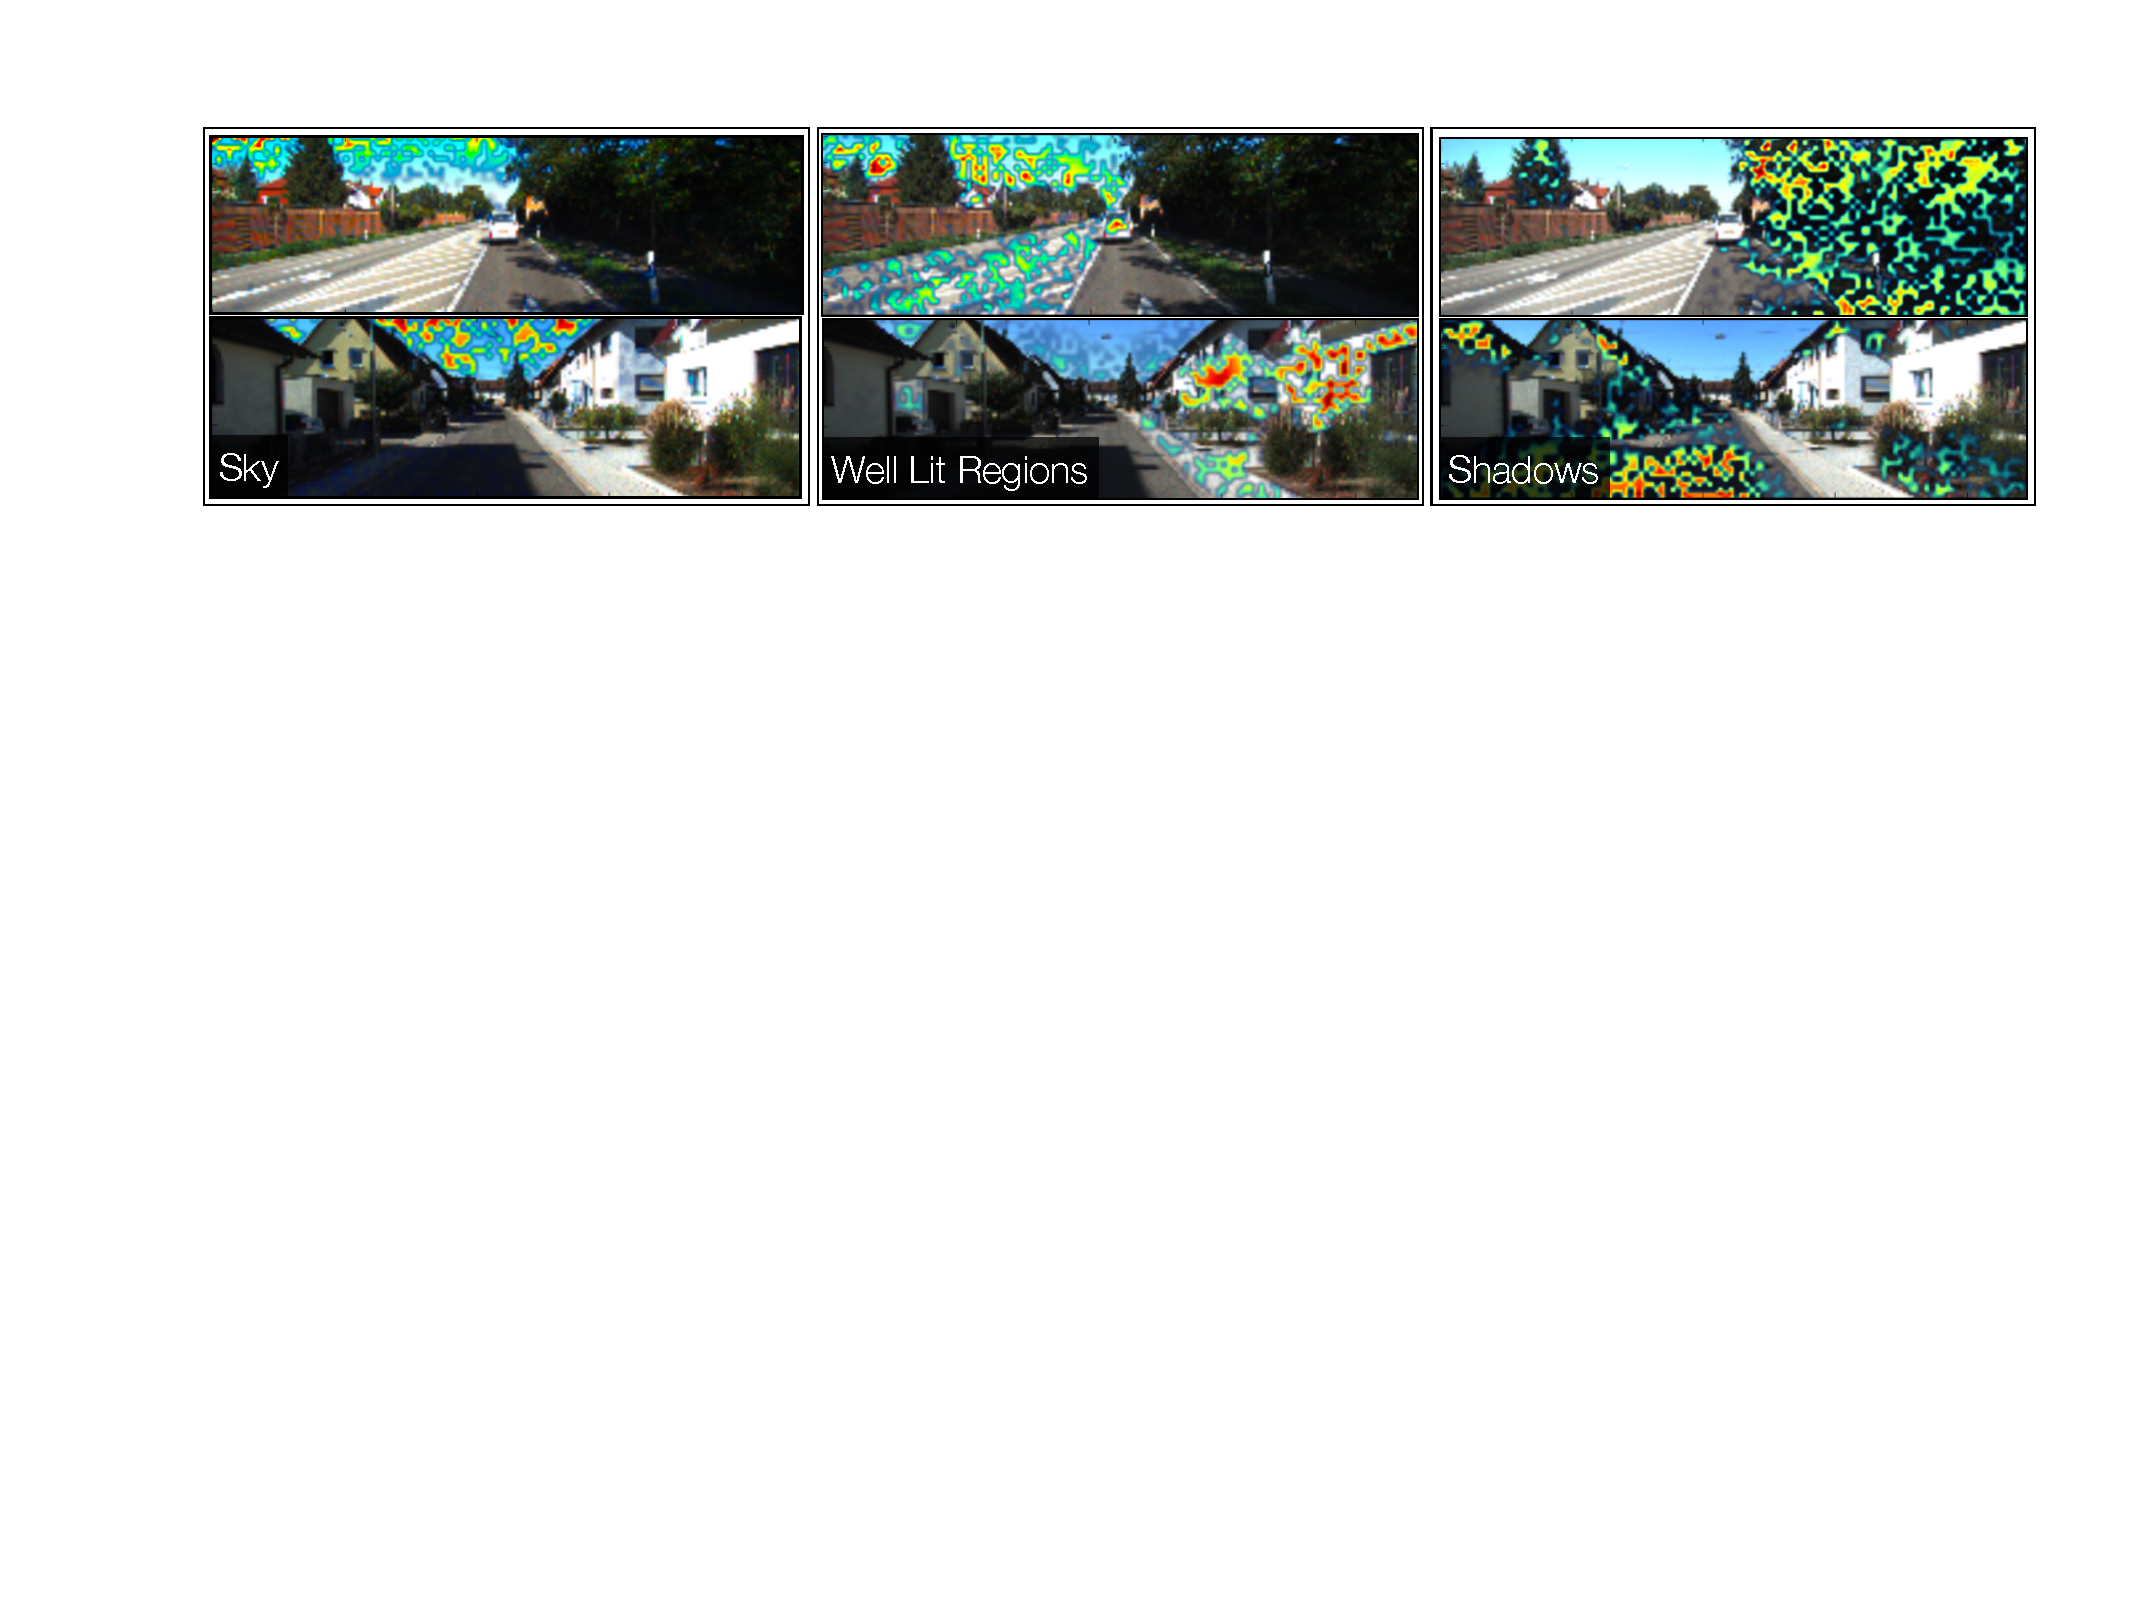
\includegraphics[width=0.98\textwidth]{sun-bcnn/kitti_activations_horiz}
    \caption{Three \texttt{conv1} layer activation maps superimposed on two images from the KITTI odometry benchmark \citep{Geiger2013-ky} \texttt{00} and \texttt{04} for three selected filters. Each filter picks out salient parts of the image that aid in sun direction inference.}
%      \vspace{-0.5em}
    \label{fig:sun-bcnn_kitti_cnn_activations}
\end{figure}

We use a Bayesian Convolutional Neural Network (BCNN) to infer the direction of the sun and an associated uncertainty, and refer to our model as Sun-BCNN. 
We motivate the choice of a deep model through the empirical findings of \citet{2017_Clement_Improving} and \citet{Ma2016-at}, who demonstrated that a CNN-based sun detector can substantially outperform hand-crafted models such as that of \citet{Lalonde2011-jw} both in terms of measurement accuracy and in its application to a VO task.

We choose a deep neural network structure based on GoogLeNet \citep{Szegedy2015-uw} due to its use in past work that adapted it for orientation regression \citep{Kendall2016-zf,Kendall2015-ew}. 
Unlike \citet{Ma2016-at}, we choose to transfer weights trained on the MIT Places dataset \citep{zhou2014MITPlaces} rather than ImageNet \citep{deng2009imagenet}.
We believe the MIT Places dataset is a more appropriate starting point for localization tasks than ImageNet since it includes outdoor scenes and is concerned with classifying physical locations rather than objects.

\subsection{Cost Function}
We train Sun-BCNN by minimizing the cosine distance between the unit-norm target sun direction vector $\SunDirection_k$  and the predicted unit-norm sun direction vector $\Estimate{\SunDirection}_k$, where $k$ indexes the images in the training set:
\begin{equation}
	\CNNLoss{\Estimate{\SunDirection}_k} = 1 - (\Estimate{\SunDirection}_k \cdot \SunDirection_k).
	\label{eq:cnn_loss}
\end{equation}
Note that in our implementation, we do not formulate the cosine distance loss explicitly, but instead minimize half the square of the tip-to-tip Euclidian distance between $\SunDirection_k$ and $\Estimate{\SunDirection}_k$, which is equivalent to \Cref{eq:cnn_loss} since both vectors have unit length:
\begin{align*}
 	\frac{1}{2} \Norm{\Estimate{\SunDirection}_k  - \SunDirection_k}^2 &= \frac{1}{2} \left( \Norm{\Estimate{\SunDirection}_k}^2 + \Norm{\SunDirection_k}^2 - 2 (\Estimate{\SunDirection}_k \cdot \SunDirection_k) \right) \\
 		&= 1 - (\Estimate{\SunDirection}_k \cdot \SunDirection_k) \\
 		&= \CNNLoss{\Estimate{\SunDirection}_k}.
\end{align*}
We ensure that our network output, $\Estimate{\SunDirection}_k$, has a unit norm by appending a normalization layer to the network.

\subsection{Uncertainty Estimation}
Following recent work on Bayesian Convolutional Neural Networks (BCNNs) \citep{Gal2016CNN,Gal2016-ny,Gal2016UncertaintyThesis}, we modify our model architecture to enable the computation of principled covariance estimates associated with each predicted sun direction. 
To achieve computationally tractable Bayesian inference with a CNN architecture, BCNNs exploit a connection between stochastic regularization (e.g., dropout, a widely used technique in deep learning to mitigate overfitting) and approximate variational inference of a Bayesian Neural Network.
We outline the technique here briefly, and refer the reader to \citet{Gal2016CNN} for more details. 

The method begins with a prior $p(\CNNVariationalWeight)$ on the weights in a deep neural network and attempts to compute a posterior distribution $p(\CNNVariationalWeight | \SunImageAll, \SunDirectionAll)$ given training inputs $\SunImageAll = \Set{\SunImage_k}$ and targets $\SunDirectionAll = \Set{\SunDirection_k}$. This posterior can be used to compute a predictive distribution for test samples but is generally intractable. To overcome this, the BCNN approach notes that CNN training with stochastic regularization can be viewed as variational inference if we define a variational distribution $q(\CNNVariationalWeight)$ as:
\begin{align}
	q(\CNNVariationalWeight_i) &= \CNNWeightAll_i \Diag{\{b^i_j\}_{j=1}^{K_i}}, \\
    b^i_j &\in \mathrm{Bernoulli}(p_i).
\end{align}
Here, $i$ indexes a particular layer in the neural network with $K_i$ weights, $\CNNWeightAll$ are the weights to be optimized, $b^i_j$ are Bernoulli distributed binary variables, and $p_i$ is the dropout probability for weights in layer $i$.

With this variational distribution $q(\CNNVariationalWeight)$, training a CNN with dropout is analogous to minimizing $\text{KL}(p(\CNNVariationalWeight | \SunImageAll, \SunDirectionAll)~||~q(\CNNVariationalWeight))$, the Kullback-Leibler (KL) divergence  between the variational distribution and the true posterior.
At test time, the first two moments of the predictive distribution are approximated using Monte Carlo integration over the weights $\CNNVariationalWeight$:
\begin{align}
\label{eq:sun_direction_mean}
\Expectation{\Optimal{\Estimate{\SunDirection}}}_k &= \Optimal{\Estimate{\Mean{\SunDirection}}}_k \approx \frac{1}{N} \sum_{n=1}^N \Optimal{\Estimate{\SunDirection}}_k (\Optimal{\SunImage}_k, \CNNVariationalWeight^n) \\
\Expectation{\Optimal{\Estimate{\SunDirection}_k} \Transpose{\Optimal{\Estimate{\SunDirection}}}_k} &\approx \tau^{-1} \IdentityMatrix 
 +  \frac{1}{N} \sum_{n=1}^N \Optimal{\Estimate{\SunDirection}}_k(\Optimal{\SunImage}_k, \CNNVariationalWeight^n) \Transpose{\Optimal{\Estimate{\SunDirection}_k}(\Optimal{\SunImage}_k, \CNNVariationalWeight^n)} \notag \\ 
 &- \Optimal{\Estimate{\Mean{\SunDirection}}}_k \Transpose{\Optimal{\Estimate{\Mean{\SunDirection}}}_k},
 \label{eq:bcnn_covar}
\end{align}
where $\IdentityMatrix$ is the identity matrix, and $\CNNVariationalWeight^n$ is a sample from $q(\CNNVariationalWeight)$ (obtained by sampling the network with dropout). The model precision, $\tau$, is computed as
\begin{equation}
	\label{eq:model_precision}
	\tau = \frac{p l^2}{2 M \lambda}, 
\end{equation} 
where $p$ is the dropout probability, $l$ is the characteristic length scale, $M$ is the number of samples in the training data, and $\lambda$ is the weight decay. 

Following \citet{Gal2016CNN}, we build our BCNN by adding dropout layers after every convolutional and fully connected layer in the network. 
We then retain these layers at test time to sample the network stochastically, following the technique of Monte Carlo Dropout, and obtain the relevant statistical quantities using \Cref{eq:bcnn_covar,eq:sun_direction_mean}. 

\subsection{Implementation and Training}
We implement our network in Caffe \citep{jia2014caffe}, using the \texttt{L2Norm} layer from the Caffe-SL fork\footnote{\url{https://github.com/wanji/caffe-sl}} to enforce a unit-norm constraint on the final output.
We train the network using stochastic gradient descent, setting all dropout probabilities to 0.5, performing 30,000 iterations with a batch size of 64, and setting the initial learning rate to be between $10^{-3}$ and $10^{-4}$. 
Training requires approximately 2.5 hours on an NVIDIA Titan X GPU.
Interestingly, \Cref{fig:sun-bcnn_kitti_cnn_activations} shows that some convolutional filters learned by Sun-BCNN on the KITTI dataset appear to correspond to illumination variations reminiscent of the visual cues designed by \citet{Lalonde2011-jw}.

\subsubsection{Data Preparation \& Transfer Learning}
We resize images from their original size to $[224 \times 224]$ pixels to achieve the image size expected by GoogleLeNet. 
We experimented with preserving the aspect ratio of the original image and padding zeros to the top and bottom of the resized image, but found that preserving the vertical resolution (as done by \citet{Ma2016-at}) results in better test-time accuracy. We do not crop or rotate the images, nor do we augment the dataset in any other way.

\subsubsection{Model Precision}
We find an empirically optimal model precision $\tau$ (see \Cref{eq:model_precision}) by optimizing the Average Normalized Estimation Error Squared (ANEES) across the entire test set for each dataset. 
While this hyperparameter should in principle be tuned using a validation set, we omit this step to keep our training procedure consistent with that of \citet{Ma2016-at}. 
We note that the BCNN uncertainty estimates are affected by two significant factors: 1) variational inference is known to underestimate predictive variance  \citep{Gal2016UncertaintyThesis}; and 2) we assume the observation noise is homoscedastic. 
As noted by \citet{Gal2016UncertaintyThesis}, the BCNN can be made heteroscedastic by learning the model precision during training, but this extension is outside the scope of this work.

\subsubsection{Data Partitioning}
    We partition our data into training and testing sets using a leave-one-out approach based on temporally disjoint sequences of images. That is, given $N$ sequences, the model tested on sequence $i$ is trained with sequences $\Set{1,2,..., N} \setminus i$. This process varies based on the dataset, and we discuss the specifics in the experimental discussion corresponding to each. In contrast to  randomly holding out a subset of the data, this method minimizes the similarity of training and testing data for temporally correlated image streams.

%%%%%%%%%%%%%%%%%%%%%%%%%%%%%%%%%%%%%%%%
% EXPERIMENTS: Simulated VO
%%%%%%%%%%%%%%%%%%%%%%%%%%%%%%%%%%%%%%%%
\section{Simulation Experiments} \label{sec:sim_vo}
\begin{figure*}
\centering
% \begin{subfigure}{0.4\textwidth}
%     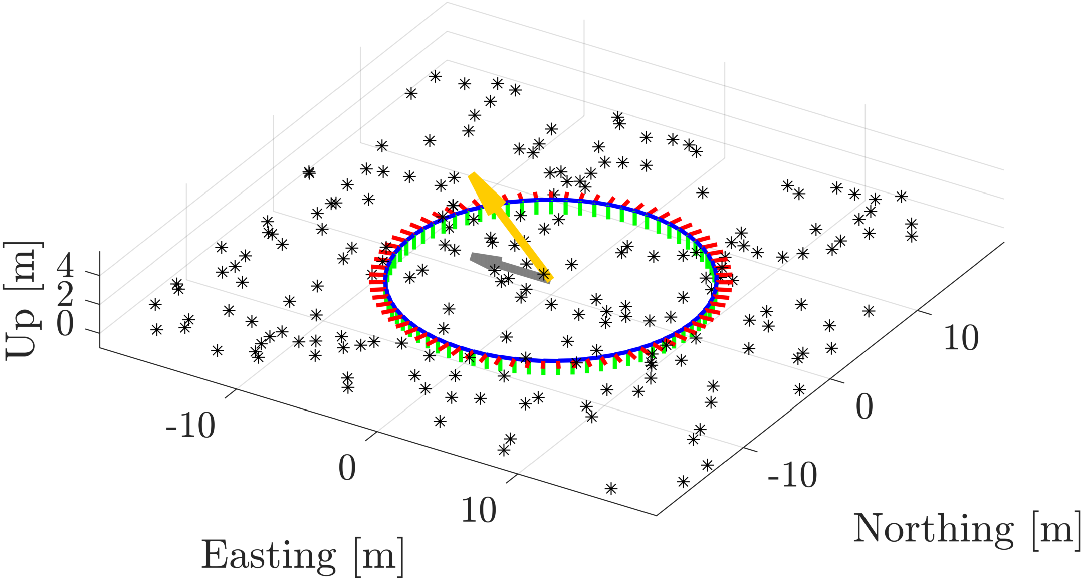
\includegraphics[width=\textwidth]{sims_circle200_environment}
%     \caption{``Circle'' trajectory}
% \end{subfigure}
\begin{subfigure}{0.45\textwidth}
    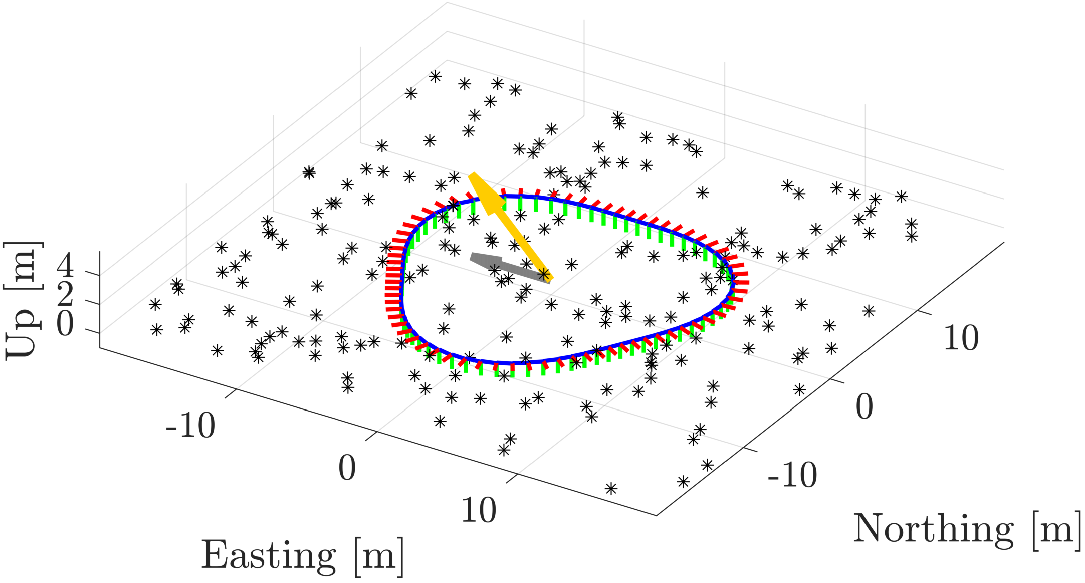
\includegraphics[width=\textwidth]{sun-bcnn/sims/sims_triangle200_environment}
    \caption{``Triangle'' trajectory}
\end{subfigure}
~
\begin{subfigure}{0.45\textwidth}
    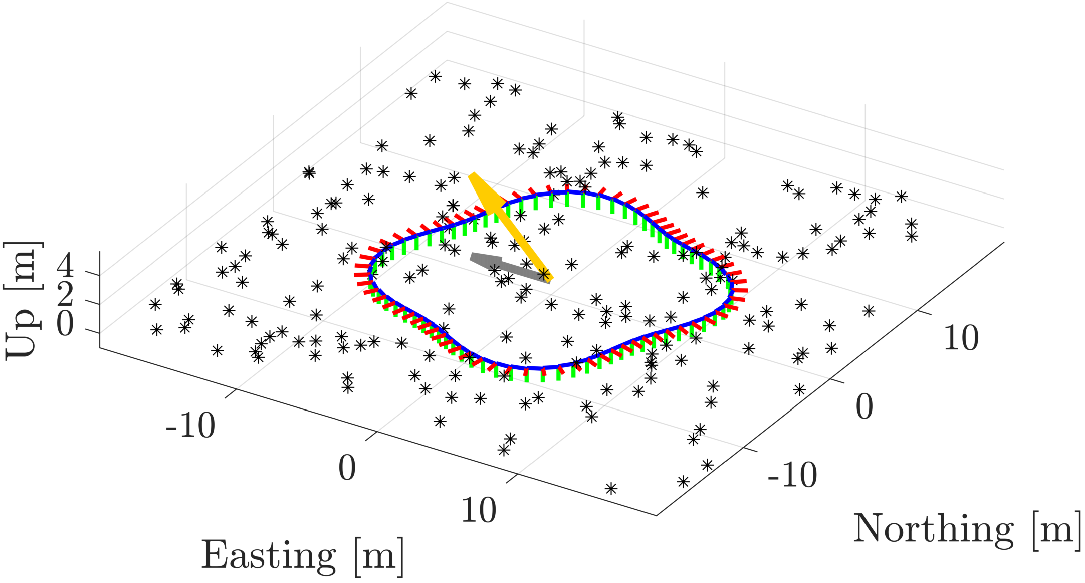
\includegraphics[width=\textwidth]{sun-bcnn/sims/sims_square200_environment}
    \caption{``Square'' trajectory}
\end{subfigure}
~
\begin{subfigure}{0.45\textwidth}
    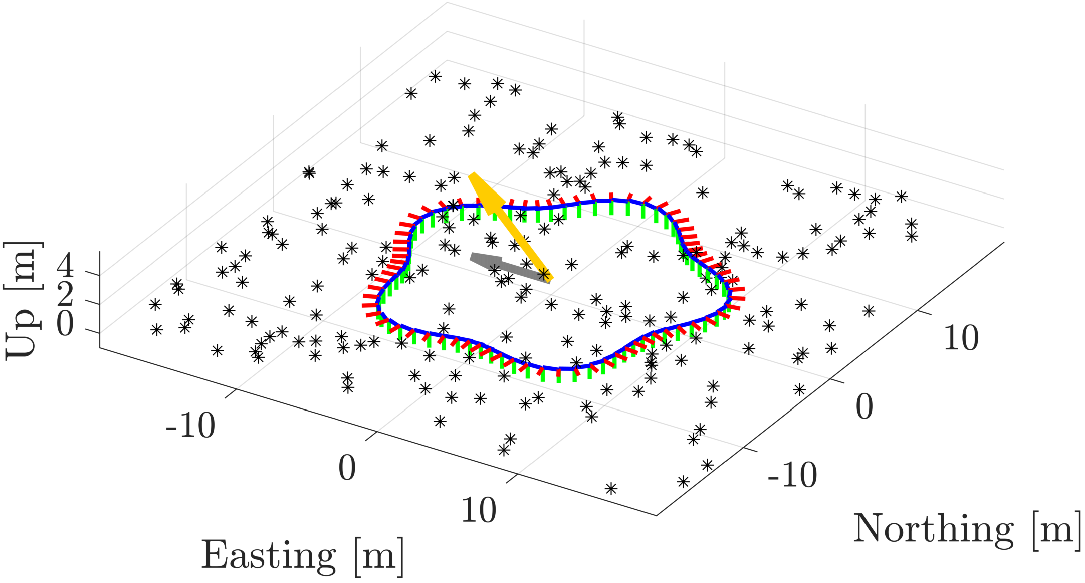
\includegraphics[width=\textwidth]{sun-bcnn/sims/sims_penta200_environment}
    \caption{``Star'' trajectory}
\end{subfigure}
\caption{One loop of the ``Triangle'', ``Square'', and ``Star'' trajectories, consisting primarily of translation and yaw rotation. Landmarks are shown as black asterisks, and the simulated sun direction is indicated with a yellow arrow along with its projection, in grey, on the EN-plane.}
\label{fig:sim_environment}
\end{figure*}

\begin{figure*}
\centering
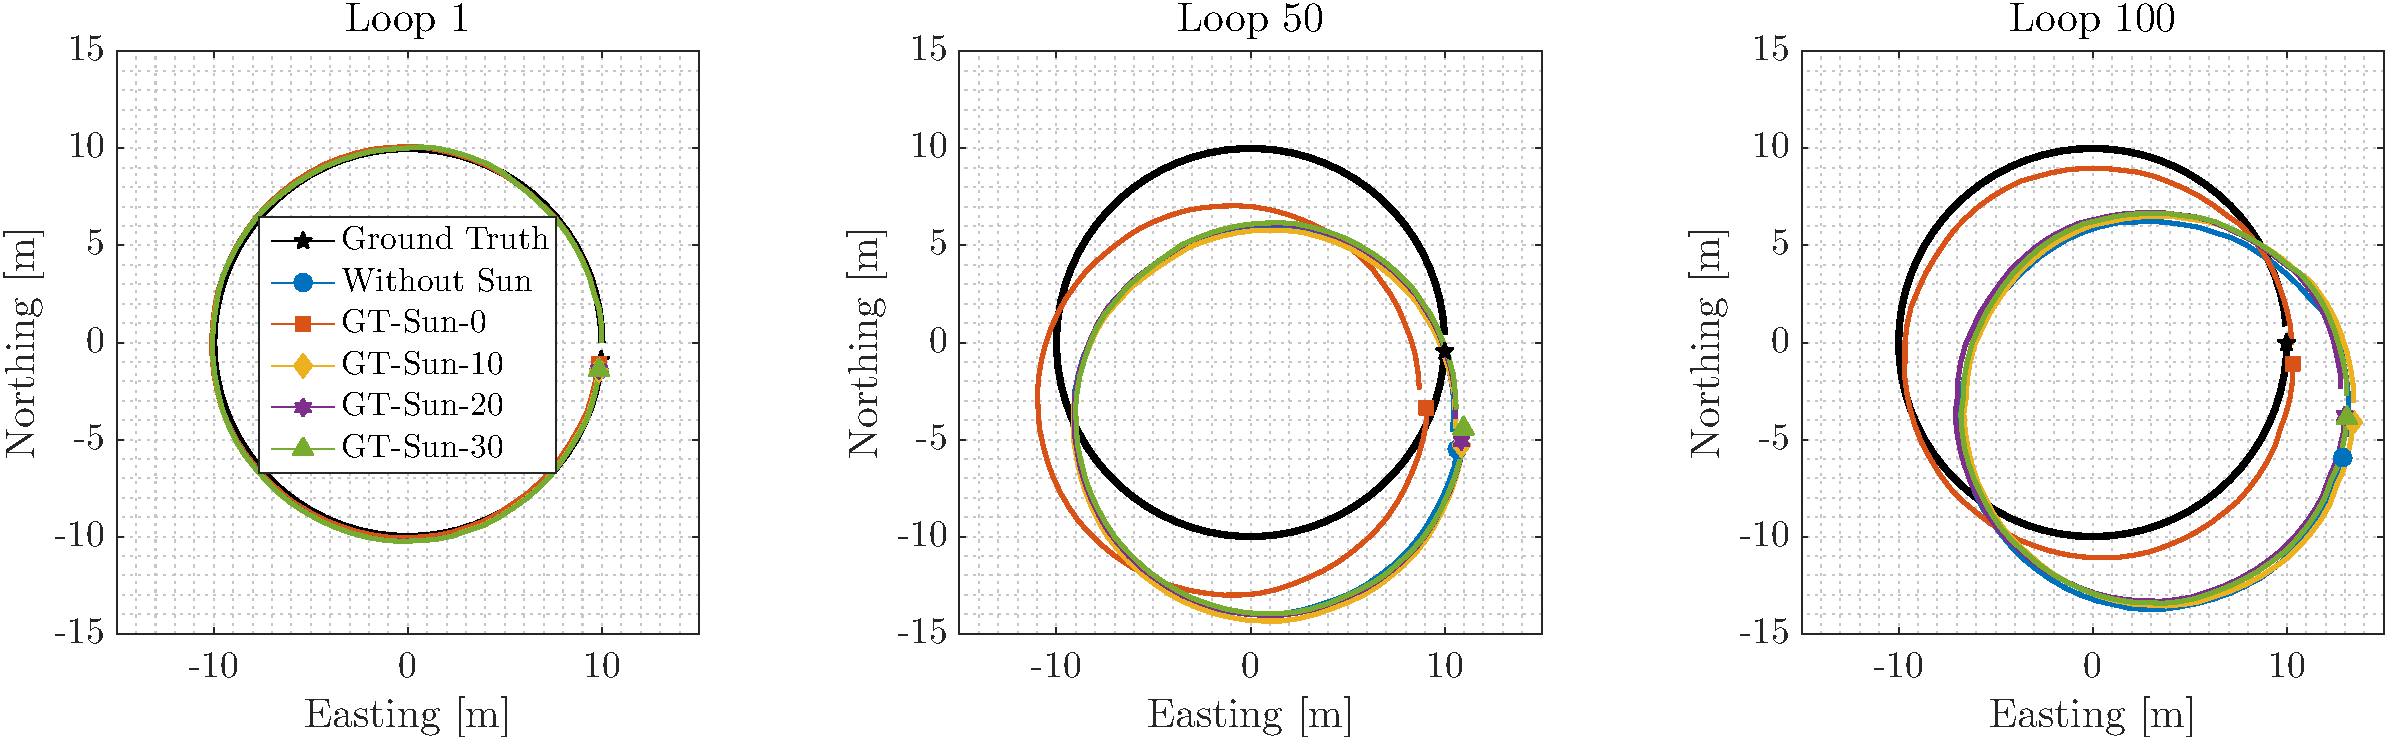
\includegraphics[width=0.98\textwidth]{sun-bcnn/sims/sims_circle200_traj}
\caption{Selected segments of a 100-loop ``Circle'' trajectory, without sun corrections, and with sun corrections corrupted by varying levels of artificial Gaussian noise. The effect of VO drift can be clearly seen, as well as the benefit of incorporating observations of a directional landmark such as the sun.}
\label{fig:sim_topdown}
\end{figure*}

\begin{figure*}
\centering
	 \begin{subfigure}{0.42\textwidth}
	 	\vspace{-5pt}
    	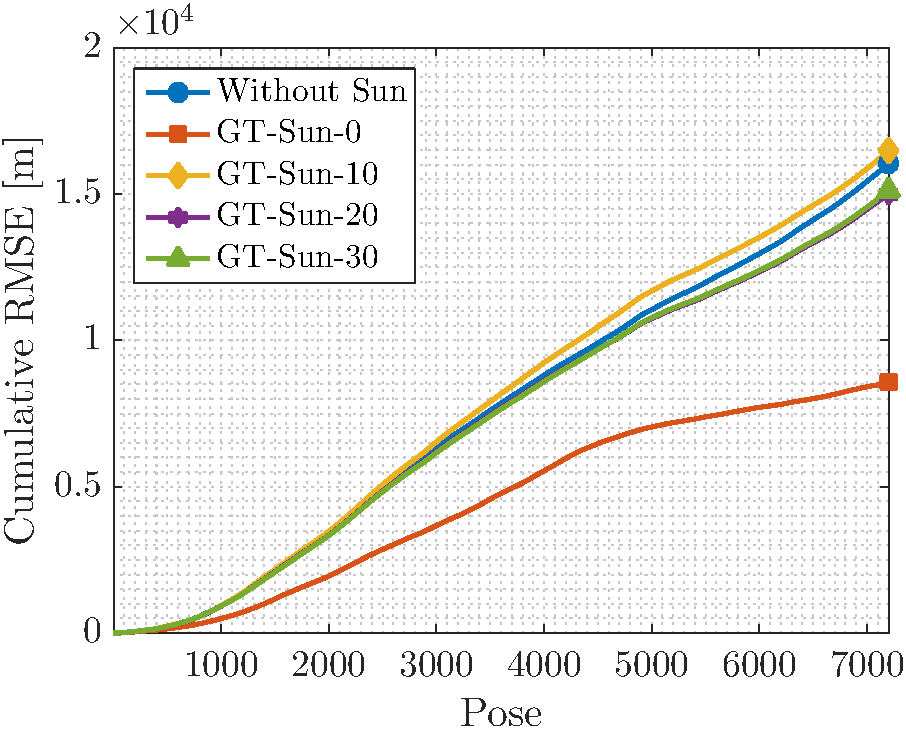
\includegraphics[width=\textwidth]{sun-bcnn/sims/sims_circle200_enu_rmse}
        \caption{Translational CRMSE (ENU)}
        \label{fig:sim_traj}
    \end{subfigure}
    ~
    \begin{subfigure}{0.42\textwidth}
    	\vspace{-5pt}
    	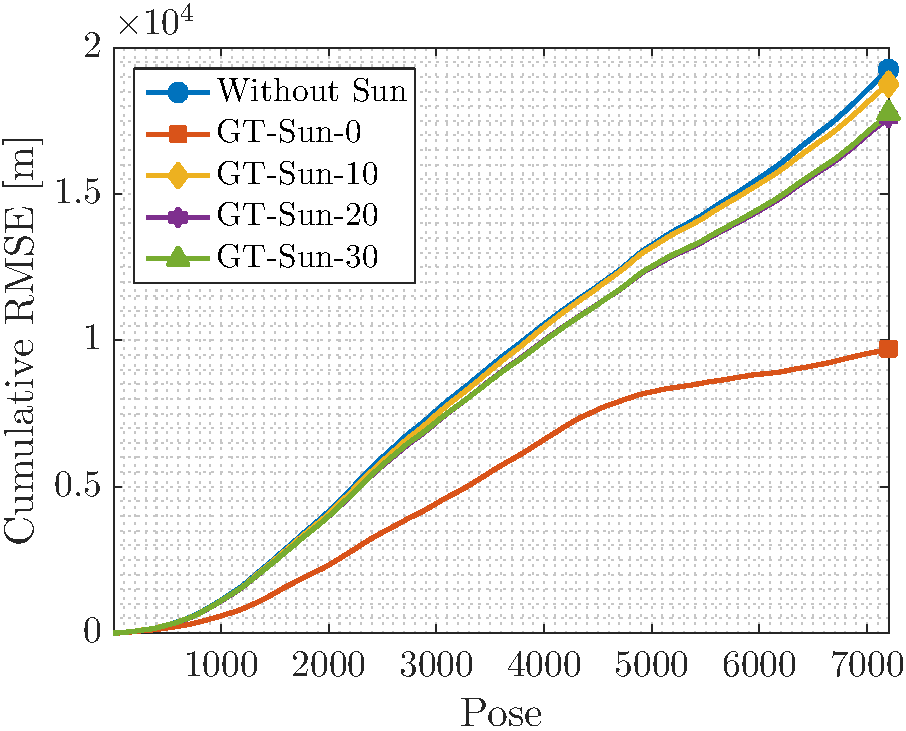
\includegraphics[width=\textwidth]{sun-bcnn/sims/sims_circle200_en_rmse}
        \caption{Translational CRMSE (EN plane)}
        \label{fig:sim_en_rmse}
    \end{subfigure}
    ~
    \begin{subfigure}{0.42\textwidth}
    	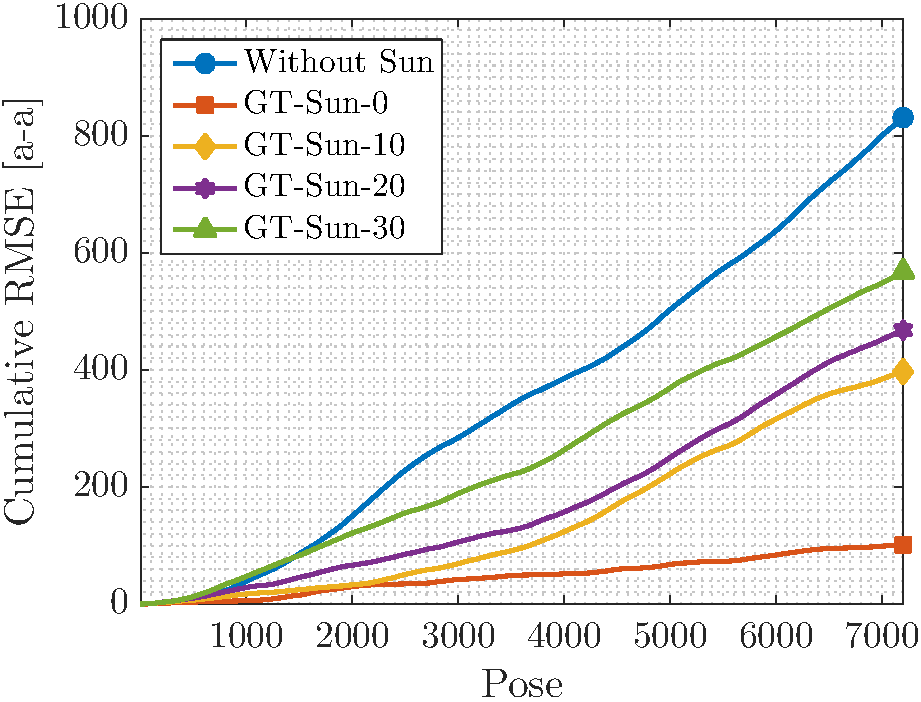
\includegraphics[width=\textwidth]{sun-bcnn/sims/sims_circle200_rot_rmse}
        \caption{Rotational CRMSE}
        \label{fig:sim_rot_rmse}
    \end{subfigure}

\caption{Cumulative root mean squared error (CRMSE) of a simulated 100-loop circular trajectory, without sun corrections, and with sun corrections corrupted by varying levels of artificial Gaussian noise. The accumulated estimation error is greatly reduced by incorporating observations of the sun, and the benefit decreases as these observations become noisier.}
\label{fig:sim_rmse}
\end{figure*}

\begin{table}[]
\centering
\caption{Comparison of translational and rotational average root mean squared errors (ARMSE) on simulated sequences.}
\label{tab:sim_armse}
\begin{tabular}{@{}lcccc@{}}
\textbf{Loop Shape}                                  & Circle & Triangle & Square & Star   \\ \midrule
\textbf{\# Loops}                             & 100    & 100      & 100    & 100    \\ \midrule
\multicolumn{5}{@{}l@{}}{\textbf{Trans. ARMSE {[}m{]}}  } \\
\quad Without Sun & 2.22 & 2.00 & 2.33 & 1.41 \T\B \\
\quad GT-Sun-0    & 1.19 & 1.62 & 2.13 & 0.75 \T \\
\quad GT-Sun-10   & 2.29 & 2.07 & 2.05 & 1.32 \\
\quad GT-Sun-20   & 2.08 & 2.12 & 2.31 & 1.33 \\
\quad GT-Sun-30   & 2.10 & 1.95 & 2.16 & 1.38 \\ \midrule
\multicolumn{5}{@{}l@{}}{\textbf{Trans. ARMSE (EN-plane) {[}m{]}}} \\
\quad Without Sun & 2.67 & 1.88 & 2.57 & 1.10 \T\B \\
\quad GT-Sun-0    & 1.34 & 1.89 & 2.56 & 0.83 \T \\
\quad GT-Sun-10   & 2.61 & 2.04 & 2.26 & 0.99 \\
\quad GT-Sun-20   & 2.44 & 2.03 & 2.57 & 0.88 \\
\quad GT-Sun-30   & 2.46 & 2.00 & 2.35 & 1.25 \\ \midrule
\multicolumn{5}{@{}l@{}}{\textbf{Rot. ARMSE $\mathbf{(\times 10^{-3})}$ {[}axis-angle{]}}} \\
\quad Without Sun & 115.32 & 144.56 & 107.27 & 111.19 \T\B \\
\quad GT-Sun-0    & 14.10  & 113.58 & 59.21  & 30.69  \T \\
\quad GT-Sun-10   & 55.22  & 115.03 & 75.62  & 39.17  \\
\quad GT-Sun-20   & 65.02  & 121.11 & 80.41  & 49.75  \\
\quad GT-Sun-30   & 78.73  & 145.22 & 100.91 & 72.39  \\ \bottomrule
\end{tabular}
\end{table}


We assess the benefit of incorporating sun observations of varying quality by conducting a series of simulation experiments consisting of a stereo camera moving along loopy trajectories of varying shapes through a simulated field of point landmarks, with a single static directional landmark representing the sun.
\Cref{fig:sim_environment} shows several such loopy trajectories.

We simulate the sun at $45^\circ$ of zenith and an arbitrary azimuth angle, and corrupt observations of the ground truth sun vector with artificial noise such that the mean angular distance (a non-negative quantity) between the observed and true sun direction is $0^\circ$, $10^\circ$, $20^\circ$, and $30^\circ$, labeling these conditions \emph{GT-Sun-0}, \emph{GT-Sun-10}, \emph{GT-Sun-20}, and \emph{GT-Sun-30}, respectively.
In our experiments, we treated the measurement noise as an additive quantity sampled from a zero-mean isotropic 3D Gaussian distribution, and renormalized the resulting vectors to enforce the unit-norm constraint.


We simulate the sun at $45^\circ$ of zenith and an arbitrary azimuth angle, and corrupt observations of the ground truth sun vector with artificial noise such that the mean angular distance (a non-negative quantity computed from the dot product) between the ground truth and noisy sun vectors is $0^\circ$, $10^\circ$, $20^\circ$, or $30^\circ$.
We label these conditions \emph{GT-Sun-0}, \emph{GT-Sun-10}, \emph{GT-Sun-20}, and \emph{GT-Sun-30}, respectively.
We generated these noisy measurements by first sampling \mbox{3-vectors} from an isotropic zero-mean multivariate Gaussian distribution, then adding these vectors to the ground truth sun vector, and finally normalizing the result to unit length. 
We chose the covariance of this distribution to yield the desired average angular distance in each case.
Note that although the distribution from which we sample noise vectors is zero-mean, the average angular distances will not be zero-mean because angular distance is non-negative.


Our choice to add noise in $\Real^3$ and re-normalize was motivated by the fact that this process yields approximately Gaussian error distributions over the azimuth and zenith error angles, which is an important property assumed by our VO pipeline to produce maximum likelihood motion estimates based on the fusion of multiple data sources.
We note that these distributions are less Gaussian-like for larger covariances (due to the geometry of the unit 2-sphere) and for ground truth vectors near singularities (e.g., zero zenith).

We also experimented with sampling simulated measurements from a Von Mises-Fisher distribution \citep{fisher1953dispersion}, which is approximately analogous to an isotropic Gaussian distribution that respects the geodesics on the unit 2-sphere.
However, we observed that the resulting distributions on azimuth and zenith error were severely non-Gaussian, which violated the assumption of zero-mean Gaussian noise in our VO pipeline and interfered with our VO experiments.

Since our VO pipeline does not incorporate loop closures, the effects of drift in the VO solution can be clearly seen by examining individual loops in the camera trajectory. 
\Cref{fig:sim_topdown} shows three loops from the ``Circle'' trajectory, demonstrating that the VO solution drifts significantly from the true trajectory by the 100th loop.
\Cref{fig:sim_rmse} plots the translational and rotational cumulative root mean squared error (CRMSE) for this trajectory, which measures the growth in total estimation error over time.
\Cref{fig:sim_rot_rmse} in particular highlights the significant effect of sun sensing on rotational error, where we see a clear progression in estimation error as the sun direction observations become more noisy.

\Cref{tab:sim_armse} shows that while all four simulation trajectories display consistent and predictable reductions in rotational average root mean squared error (ARMSE), this is not always the case for translational ARMSE.
This is because translational errors are only partially induced by rotational errors, with the remainder made up of `sliding' motions orthogonal to the direction of travel.
These non-rotational errors are highly dependent on the specific trajectory, where more or less of the observed feature tracks can be explained by a sliding motion instead of a rotation.
Due to the coupling of translational and rotational errors, correcting for rotational error in such cases may actually worsen the translational error (e.g., on the ``Triangle'' sequence).

While we do not implement this in our work, we speculate that incorporating an appropriate motion model into our VO formulation would significantly mitigate the impact of these errors by, for example, imposing a nonholonomic constraint on a ground vehicle or accounting for the dynamics of a quadcopter.

%%%%%%%%%%%%%%%%%%%%%%%%%%%%%%%%%%%%%%%%
% EXPERIMENTS: KITTI
%%%%%%%%%%%%%%%%%%%%%%%%%%%%%%%%%%%%%%%%
\section{Urban Driving Experiments: The KITTI Odometry Benchmark}
\begin{figure}
    \centering
    \begin{subfigure}[b]{0.75\textwidth}
        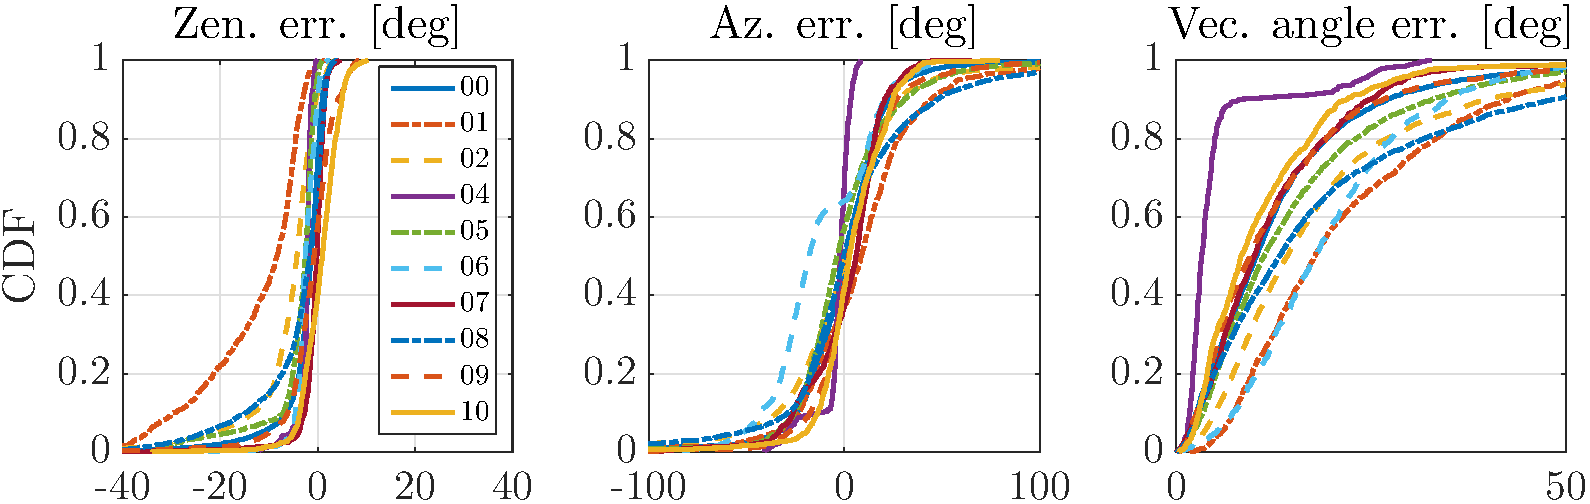
\includegraphics[width=\textwidth]{sun-bcnn/kitti/kitti_cdf}
    \end{subfigure} ~
    \begin{subfigure}[b]{0.75\textwidth}
        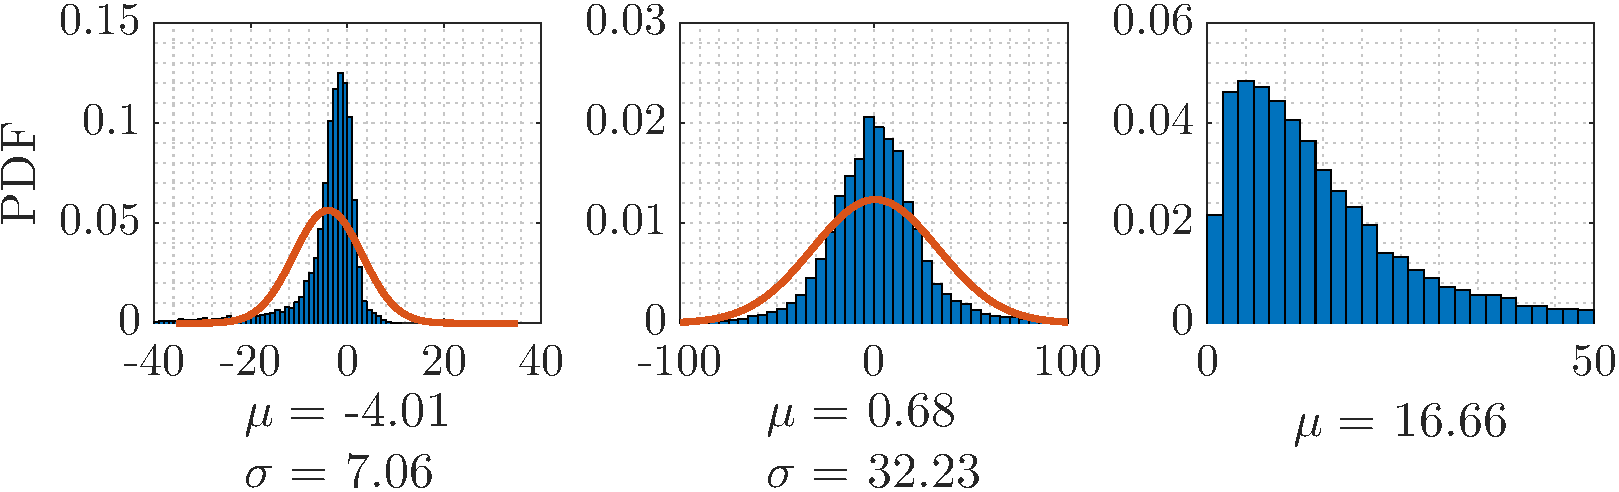
\includegraphics[width=\textwidth]{sun-bcnn/kitti/kitti_hist_azzen}
    \end{subfigure}
    \caption{Distributions of azimuth error, zenith error, and angular distance for Sun-BCNN compared to ground truth over each test sequence in the KITTI dataset. \emph{Top row}: Cumulative distributions of errors for each test sequence individually. \emph{Bottom row:} Histograms and Gaussian fits of aggregated errors.}
    \label{fig:sun-bcnn_kitti_cnn_testerrors}
\end{figure}

\begin{figure}
    \centering
    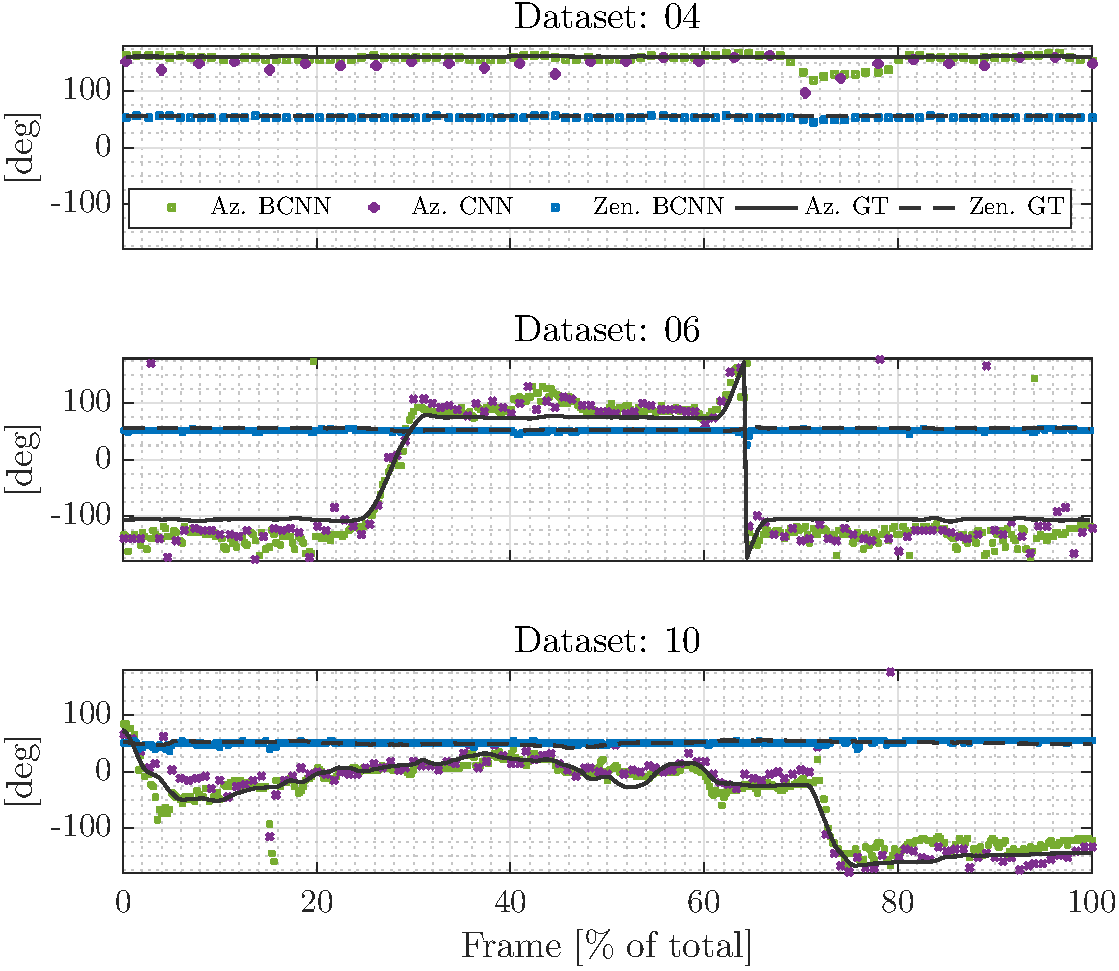
\includegraphics[width=0.75\textwidth]{sun-bcnn/kitti/kitti_error_over_time}
    \caption{Azimuth (Sun-CNN and Sun-BCNN) and zenith (Sun-BCNN only) predictions over time for KITTI test sequences \texttt{04}, \texttt{06} and \texttt{10}. Sun-CNN is trained and tested on every tenth image, whereas Sun-BCNN is trained and tested on every image. In our VO experiments, we use the Sun-BCNN predictions of every tenth image to make a fair comparison. }
    %\vspace{-0.4em}
    \label{fig:sun-bcnn_kitti_error_over_time}
\end{figure}

\begin{table}
\centering
\caption{Test Errors for Sun-BCNN on KITTI odometry sequences with estimates computed at every image.}
\resizebox{\columnwidth}{!}{%
\label{tab:kitti_test_cnn}
\begin{threeparttable}
\begin{tabular}{@{}cccccccccccccccc@{}}
         &  & \multicolumn{3}{c}{\textbf{Zenith Error {[}deg{]}}} &  & \multicolumn{3}{c}{\textbf{Azimuth Error {[}deg{]}}} &  & \multicolumn{3}{c}{\textbf{Vector Angle Error {[}deg{]}}} & & \B \\ \cline{3-5} \cline{7-9} \cline{11-13} 
\textbf{Sequence} &  & Mean          & Median       & Stdev       &  & Mean         & Median        & Stdev        &  & Mean           & Median          & Stdev & & \textbf{ANEES}\tnote{1}         \T \\ \midrule
\texttt{00}     &  & -2.59  & -1.37  & 5.15           &  & -0.33  & 0.81   & 25.61           &  & 13.56 & 10.31  & 13.14 &  & 1.00 \T \\
\texttt{01}     &  & -12.53 & -8.31  & 10.33          &  & 8.95   & 8.83   & 33.67           &  & 22.16 & 17.85  & 15.00 &  & 1.38 \\
\texttt{02}     &  & -6.13  & -4.26  & 7.38           &  & -1.03  & 0.74   & 37.61           &  & 19.69 & 14.32  & 18.25 &  & 1.40 \\
\texttt{04}     &  & -2.42  & -2.11  & 1.64           &  & -3.89  & -2.18  & 9.14            &  & 5.33  & 3.29   & 6.44  &  & 0.30 \\
\texttt{05}     &  & -4.31  & -2.51  & 6.18           &  & -0.74  & -3.80  & 29.81           &  & 15.66 & 11.33  & 14.80 &  & 1.05 \\
\texttt{06}     &  & -2.48  & -2.52  & 2.27           &  & -12.22 & -17.86 & 25.78           &  & 19.78 & 17.72  & 11.35 &  & 1.93 \\
\texttt{07}     &  & -0.69  & -0.16  & 3.26           &  & 1.25   & 5.98   & 20.27           &  & 12.44 & 10.05  & 9.97  &  & 0.97 \\
\texttt{08}     &  & -4.46  & -1.61  & 8.14           &  & 3.66   & -0.14  & 41.73           &  & 19.90 & 13.30  & 19.59 &  & 1.04 \\
\texttt{09}     &  & -1.35  & -0.75  & 5.60           &  & 4.78   & 2.36   & 23.84           &  & 13.09 & 9.48   & 12.66 &  & 0.73 \\
\texttt{10}     &  & 0.59   & 0.95   & 3.90           &  & 3.64   & 2.61   & 19.15           &  & 11.23 & 8.34   & 9.83  &  & 1.08 \B \\ \midrule
All                &  & -4.01  & -2.26  & 7.06           &  & 0.68   & 0.53   & 32.23           &  & 16.66 & 12.08  & 15.91 & & - &  \\ \bottomrule    
\end{tabular}
\begin{tablenotes}
	\item[1] We compute Average Normalized Estimation Error Squared (ANEES) values with all sun directions that fall below a cosine distance threshold of $0.3$ (relative to ground truth) and set $\tau^{-1} = 0.015$.
 \end{tablenotes}
\end{threeparttable}
}
\end{table}

\begin{figure}
    \centering
    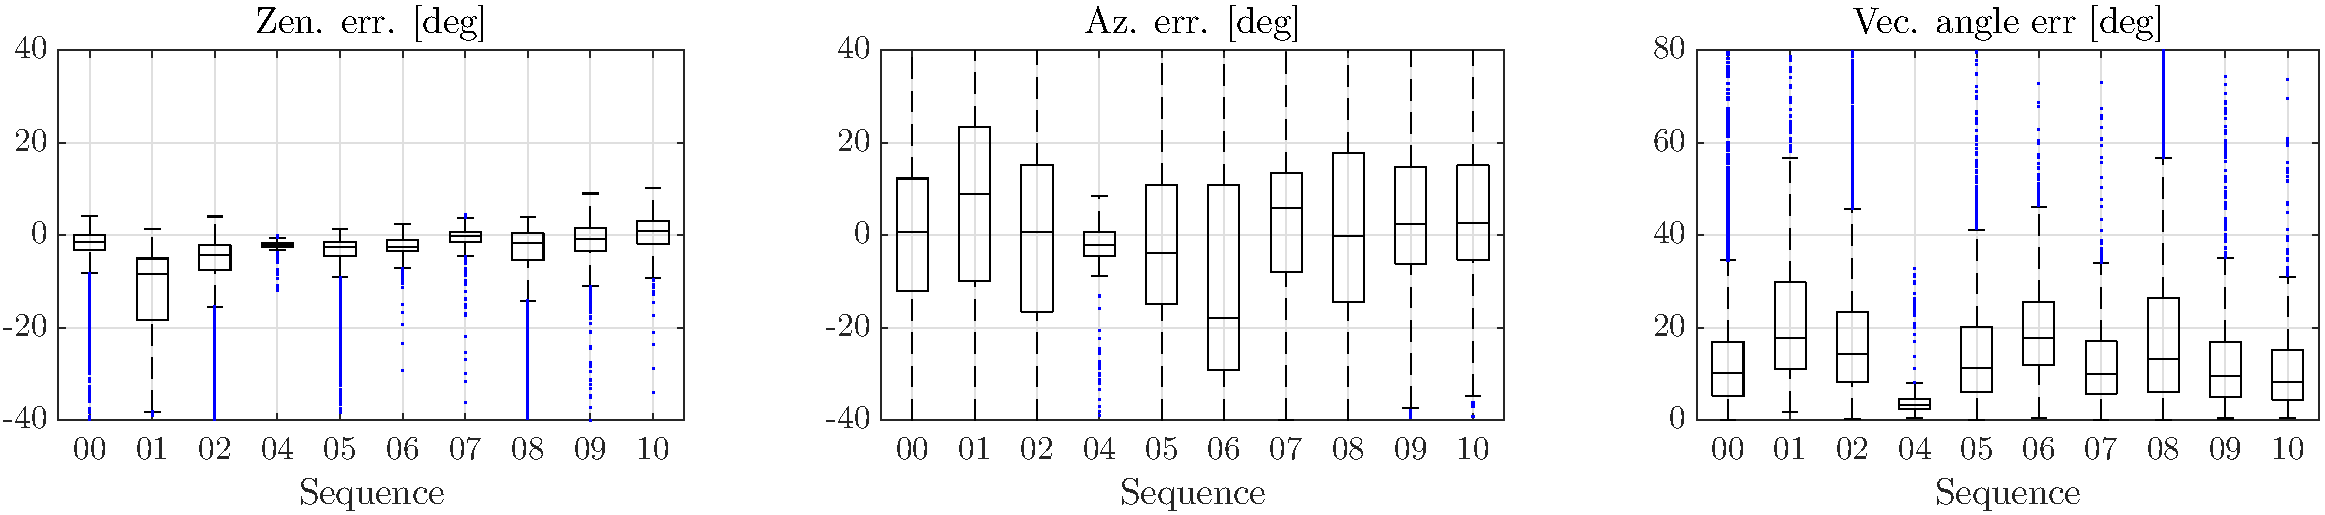
\includegraphics[width=0.98\textwidth]{sun-bcnn/kitti/kitti_testStatsBoxPlot}
    \caption{Box-and-whiskers plot of final test errors on all ten KITTI odometry sequences (c.f. \Cref{tab:kitti_test_cnn}).}
%    \vspace{-0.4em}
    \label{fig:kitti_test_error_whiskers}
\end{figure}

\begin{figure}
	\centering
	 \begin{subfigure}{0.42\textwidth}
    	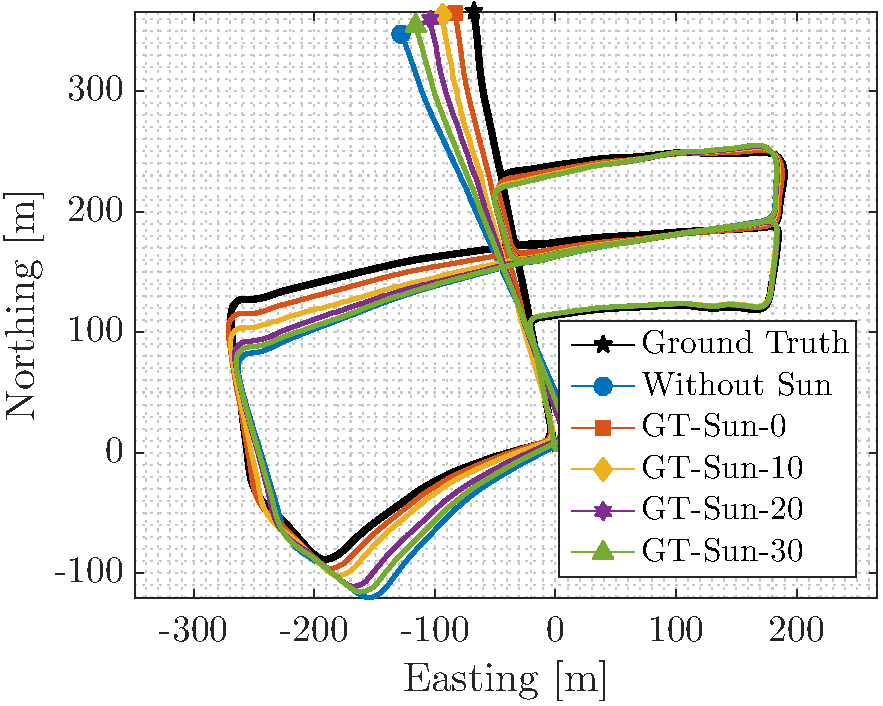
\includegraphics[width=\textwidth]{sun-bcnn/kitti/kitti_05_traj_sim}
        \caption{VO and ground truth trajectories}
    \end{subfigure}
    ~
    \begin{subfigure}{0.42\textwidth}
    	\vspace{-8pt}
    	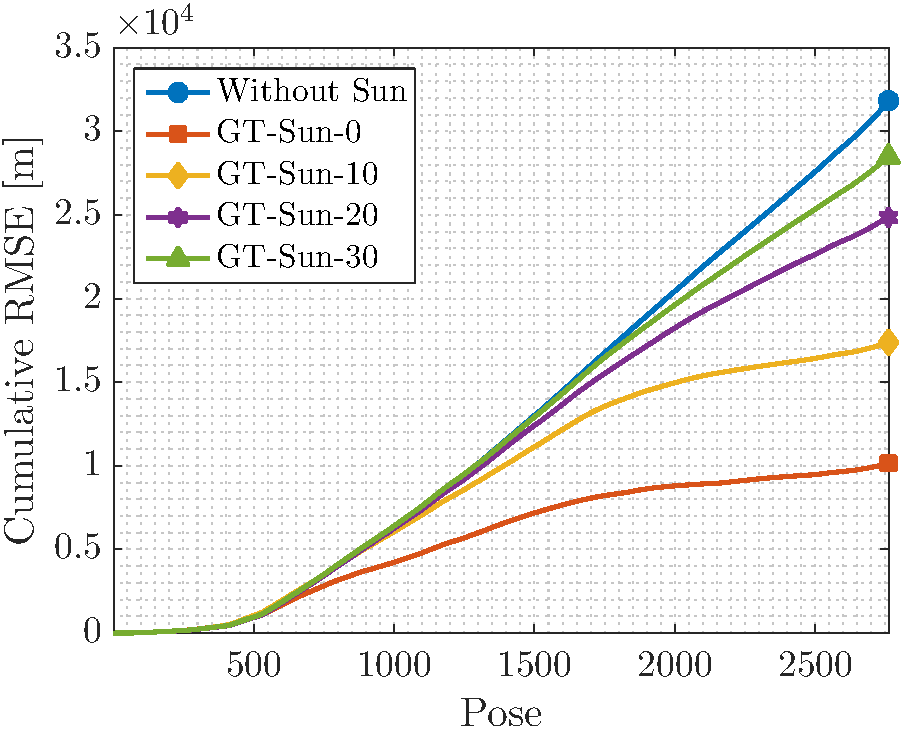
\includegraphics[width=\textwidth]{sun-bcnn/kitti/kitti_05_en_rmse_sim}
        \caption{Translational CRMSE (EN-plane)}
    \end{subfigure}
    ~
    \begin{subfigure}{0.42\textwidth}
    	\includegraphics[width=\textwidth]{sun-bcnn/kitti/kitti_05_rot_rmse_sim}
        \caption{Rotational CRMSE}
    \end{subfigure}

    \caption{VO results for KITTI odometry sequence \texttt{05} using simulated sun measurements at every tenth pose. We observe a clear progression in cumulative root mean squared error (CRMSE) in translation and rotation as noise in the simulated sun measurements increases.}
     \label{fig:kitti-vo-sim-results}
\end{figure}

We investigated the performance of Sun-BCNN on the KITTI odometry benchmark training set \citep{Geiger2013-ky}, which consists of 21.6 km of urban driving data\footnote{Because we rely on the first pose reported by the GPS/INS system, we used the raw (rectified and synchronized) sequences corresponding to each odometry sequence. However, the raw sequence \texttt{2011\_09\_26\_drive\_0067} corresponding to odometry sequence \texttt{03} was not available on the KITTI website at the time of writing, so we omit sequence \texttt{03} from our analysis.}.
Importantly, the dataset includes 6-DOF ground truth poses obtained from an accurate GPS/INS tracking system, as well as calibrated transformations between this sensor and the colour stereo pair we use for sun estimation and VO in our experiments.
This allows us to create a training set of ground truth sun vectors for each image by querying the solar ephemeris model at each ground truth pose and rotating the resulting vector from the GPS/INS frame $\CoordinateFrame{0}$ (which is an ENU coordinate system) into the camera coordinate frame $\CoordinateFrame{k}$.
For each of our experiments, we trained Sun-BCNN on nine benchmark sequences and tested on the remaining sequence.
This procedure is consistent with that of \citet{Ma2016-at}, against whose Sun-CNN we directly compare, and allows us to evaluate each sequence using the maximum amount of training data.

\begin{figure*}[h]
	\centering
	\includegraphics[width=0.82\textwidth]{sun-bcnn/kitti/kitti_kitti_arrow_fig}	
	\caption{Sun BCNN predictions and associated ground truth sun directions on the KITTI sequence \texttt{05}. \emph{Top two rows}: Sun BCNN produces accurate predictions in a variety of azimuth values. \emph{Bottom row}: Poor results occur rarely due to shadow ambiguities.}
	\label{fig:kitti_arrows}
\end{figure*}

\begin{figure*}
	\centering
	 \begin{subfigure}{0.3\textwidth}
    	\includegraphics[width=\textwidth]{sun-bcnn/kitti/kitti_02_traj}
        \caption{\texttt{02}: VO and ground truth trajectories}
    \end{subfigure}
    ~
    \begin{subfigure}{0.3\textwidth}
    	\includegraphics[width=\textwidth]{sun-bcnn/kitti/kitti_05_traj}
        \caption{\texttt{05}: VO and ground truth trajectories}
    \end{subfigure}
    ~
    \begin{subfigure}{0.3\textwidth}
    	\includegraphics[width=\textwidth]{sun-bcnn/kitti/kitti_08_traj}
        \caption{\texttt{08}: VO and ground truth trajectories}
    \end{subfigure}
    \\
    \begin{subfigure}{0.3\textwidth}
    	\includegraphics[width=\textwidth]{sun-bcnn/kitti/kitti_02_en_rmse}
        \caption{\texttt{02}: Translational CRMSE (EN-plane)}
    \end{subfigure}
    ~
    \begin{subfigure}{0.3\textwidth}
    	\includegraphics[width=\textwidth]{sun-bcnn/kitti/kitti_05_en_rmse}
        \caption{\texttt{05}: Translational CRMSE (EN-plane)}
    \end{subfigure}
    ~
    \begin{subfigure}{0.3\textwidth}
    	\includegraphics[width=\textwidth]{sun-bcnn/kitti/kitti_08_en_rmse}
        \caption{\texttt{08}: Translational CRMSE (EN-plane)}
    \end{subfigure}
    \\
    \begin{subfigure}{0.3\textwidth}
    	\includegraphics[width=\textwidth]{sun-bcnn/kitti/kitti_02_rot_rmse}
        \caption{\texttt{02}: Rotational CRMSE}
    \end{subfigure}
    ~
    \begin{subfigure}{0.3\textwidth}
    	\includegraphics[width=\textwidth]{sun-bcnn/kitti/kitti_05_rot_rmse}
        \caption{\texttt{05}: Rotational CRMSE}
    \end{subfigure}
    ~
    \begin{subfigure}{0.3\textwidth}
    	\includegraphics[width=\textwidth]{sun-bcnn/kitti/kitti_08_rot_rmse}
        \caption{\texttt{08}: Rotational CRMSE}
    \end{subfigure}
    
    \caption{VO results for KITTI odometry sequences \texttt{02}, \texttt{05}, and \texttt{08} using estimate sun directions at every tenth pose. \emph{Top row}: Estimated and ground truth trajectories in the Easting-Northing (EN) plane. \emph{Middle row}: Translational cumulative root mean squared error (CRMSE) in the EN-plane. \emph{Bottom row}: Rotational CRMSE. Sun-BCNN significantly reduces the estimation error on sequence \texttt{05}, while the Lalonde \citep{Lalonde2011-jw}, Lalonde-VO \citep{2017_Clement_Improving}, and Sun-CNN \citep{Ma2016-at} methods provide modest reductions in estimation error. The remaining sequences are less clear, but Sun-BCNN generally provides some benefit.}
     \label{fig:kitti-vo-results}
\end{figure*}

\begin{table}[]
\centering
\caption{Comparison of translational and rotational average root mean squared error (ARMSE) on KITTI odometry sequences with and without sun direction estimates at every tenth image. The best result (excluding simulated sun sensing) is highlighted in bold.}
\resizebox{\columnwidth}{!}{%
\label{tab:sun-bcnn_kitti_armse}
\begin{threeparttable}
\begin{tabular}{@{}lcccccccccc@{}}
\textbf{Sequence}\tnote{1}     & \texttt{00} & \texttt{01}\tnote{2} & \texttt{02} & \texttt{04} & \texttt{05} & \texttt{06} & \texttt{07} & \texttt{08} & \texttt{09} & \texttt{10} \\ \midrule
\textbf{Length {[}km{]}}       & 3.7   & 2.5    & 5.1   & 0.4  & 2.2   & 1.2   & 0.7   & 3.2   & 1.7   & 0.9   \\ \midrule
\multicolumn{11}{@{}l@{}}{\textbf{Trans. ARMSE {[}m{]}}} \\
\quad Without Sun & 4.33          & 198.52          & 28.59          & 2.48          & 9.90          & 3.35          & 4.55          & 28.05          & 10.44          & 5.54          \T\B \\
\quad GT-Sun-0    & 5.40          & 114.69          & 23.83          & 2.23          & 4.84          & 3.50          & 1.58          & 31.55          & 8.21           & 3.67          \T \\
\quad GT-Sun-10   & 4.85          & 123.84          & 25.34          & 2.45          & 5.84          & 2.80          & 2.94          & 28.47          & 8.65           & 4.81          \\
\quad GT-Sun-20   & 4.78          & 136.60          & 22.33          & 2.46          & 8.16          & 3.03          & 3.90          & 27.54          & 8.68           & 5.45          \\
\quad GT-Sun-30   & 4.83          & 157.14          & 27.30          & 2.48          & 8.93          & 3.44          & 4.62          & 26.73          & 10.10          & 5.28          \B \\
\quad Lalonde     & \textbf{3.81} & 200.34          & 28.13          & \textbf{2.47} & 9.88          & 3.36          & 4.61          & 29.70          & 10.49          & \textbf{5.48} \T \\
\quad Lalonde-VO  & 4.87          & 199.03          & 29.41          & 2.48          & 9.74          & \textbf{3.30} & 4.52          & 27.82          & 11.06          & 5.59          \B \\
\quad Sun-CNN     & 4.36          & 192.50          & \textbf{26.58} & 2.48          & 8.92          & 3.38          & 4.30          & \textbf{26.99} & 10.15          & 5.58          \T \\
\quad Sun-BCNN    & 4.44          & \textbf{188.46} & 26.89          & 2.48          & \textbf{8.50} & 4.10          & \textbf{4.21} & 27.71          & \textbf{10.13} & 5.61          \\ \midrule
\multicolumn{11}{@{}l@{}}{\textbf{Trans. ARMSE (EN-plane) {[}m{]}}} \\
\quad Without Sun & 4.53          & 230.73          & 30.66          & 1.81          & 11.50         & 3.68          & 5.44          & 32.37          & 11.65          & 5.95          \T\B \\
\quad GT-Sun-0    & 3.41          & 136.76          & 24.12          & 1.46          & 3.67          & 3.96          & 1.80          & 21.51          & 7.77           & 3.71          \T \\
\quad GT-Sun-10   & 5.05          & 149.36          & 24.79          & 1.79          & 6.29          & 2.73          & 3.51          & 22.41          & 8.90           & 5.09          \\
\quad GT-Sun-20   & 5.14          & 164.37          & 22.04          & 1.80          & 9.01          & 3.13          & 4.66          & 27.58          & 8.86           & 5.81          \\
\quad GT-Sun-30   & 5.12          & 188.61          & 22.65          & 1.83          & 10.31         & 3.83          & 5.50          & 27.65          & 11.16          & 5.58          \B \\
\quad Lalonde     & \textbf{3.95} & 232.66          & 27.30          & \textbf{1.81} & 11.20         & 3.70          & 5.52          & 27.84          & 11.41          & \textbf{5.87} \T \\
\quad Lalonde-VO  & 5.38          & 231.33          & 33.68          & 1.82          & 11.13         & \textbf{3.61} & 5.42          & 32.24          & 12.41          & 6.00          \B \\
\quad Sun-CNN     & 4.56          & 224.91          & 24.65          & 1.82          & 9.99          & 3.74          & 5.16          & 30.09          & 11.21          & 5.99          \T \\
\quad Sun-BCNN    & 4.68          & \textbf{220.54} & \textbf{23.58} & 1.82          & \textbf{6.70} & 4.78          & \textbf{5.05} & \textbf{26.59} & \textbf{10.97} & 6.03          \\ \midrule
\multicolumn{11}{@{}l@{}}{\textbf{Rot. ARMSE $\mathbf{(\times 10^{-3})}$ {[}axis-angle{]}}} \\
\quad Without Sun & 23.88          & 185.30          & 63.18          & 12.97          & 70.18          & 23.24          & 49.96          & 63.13          & 26.77          & 21.54          \T\B \\
\quad GT-Sun-0    & 11.20          & 38.82           & 53.48          & 11.75          & 29.38          & 17.66          & 20.37          & 56.39          & 17.00          & 12.60          \T \\
\quad GT-Sun-10   & 17.05          & 64.51           & 58.78          & 12.86          & 41.47          & 18.90          & 34.05          & 54.89          & 19.71          & 14.26          \\
\quad GT-Sun-20   & 18.84          & 94.65           & 58.03          & 12.91          & 55.39          & 19.67          & 43.34          & 58.82          & 20.99          & 25.87          \\
\quad GT-Sun-30   & 23.40          & 121.21          & 57.79          & 13.01          & 62.73          & 23.96          & 49.92          & 56.74          & 25.63          & 20.15          \B \\
\quad Lalonde     & \textbf{21.10} & 188.06          & 66.02          & \textbf{12.96} & 69.00          & 23.27          & 50.49          & 64.22          & 26.27          & \textbf{20.49} \T \\
\quad Lalonde-VO  & 27.91          & 185.52          & 69.52          & 12.98          & 68.09          & \textbf{22.79} & 49.74          & 65.35          & 28.82          & 22.10          \B \\
\quad Sun-CNN     & 24.05          & 177.45          & \textbf{58.32} & 13.00          & 61.48          & 23.34          & 47.77          & \textbf{60.55} & \textbf{26.19} & 21.99          \T \\
\quad Sun-BCNN    & 26.96          & \textbf{175.21} & 75.02          & 13.00          & \textbf{47.96} & 23.80          & \textbf{47.57} & 62.85          & 26.29          & 20.85          \\ \bottomrule
\end{tabular}
\begin{tablenotes}
	\item[1] Because we rely on the timestamps and first pose reported by the GPS/INS system, we use the raw (rectified and synchronized) sequences corresponding to each odometry sequence. However, the raw sequence \texttt{2011\_09\_26\_drive\_0067} corresponding to odometry sequence \texttt{03} was not available on the KITTI website at the time of writing, so we omit sequence \texttt{03} from our analysis.
    \item[2] Sequence \texttt{01} consists largely of self-similar, corridor-like highway driving which causes difficulties when detecting and matching features using \texttt{libviso2}. The base VO result is of low quality, although we note that including global orientation from the sun nevertheless improves the VO result.
\end{tablenotes}
\end{threeparttable}
}
\end{table}

\subsection{Sun-BCNN Test Results}
Once trained, we analyzed the accuracy and consistency of the Sun-BCNN mean and covariance estimates.
We obtained the mean estimated sun vector by evaluating \Cref{eq:sun_direction_mean} with $N=25$ and then re-normalized the resulting vector to preserve unit length. 
To obtain the required covariance on azimuth and zenith angles, we sampled the vector outputs, converted them to azimuth and zenith angles using \Cref{eq:vec-to-az-zen}, and then applied \Cref{eq:bcnn_covar}.
We investigate the impact of this parametrization (as opposed to working in azimuth and zenith coordinates directly) later in this paper.
As shown in \Cref{tab:kitti_test_cnn}, we chose a value for the model precision $\tau$ such that the Average Normalized Estimation Error Squared (ANEES) of each test sequence is close to one (i.e., the estimator is consistent).

\Cref{fig:kitti_test_error_whiskers,fig:sun-bcnn_kitti_cnn_testerrors} plot the error distributions for azimuth, zenith, and angular distance for all ten KITTI odometry sequences, while \Cref{fig:sun-bcnn_kitti_error_over_time} shows three characteristic plots of the azimuth and zenith predictions over time. 
We see that the errors in azimuth and zenith are strongly peaked around zero and are reasonably well described by a Gaussian distribution, which are important properties assumed by our VO pipeline to produce maximum likelihood motion estimates based on the fusion of multiple data sources.
Note that the error distribution in zenith is slightly biased towards negative values due to the presence of a long tail on the negative side of the mean.
This is an artifact of the azimuth-zenith parameterization when the sun zenith is small (i.e., when the sun is high in the sky), since zenith angles are defined on $[0,\pi]$.
In practice, we attempt to reduce the influence of the long negative tail by imposing a robust Huber loss on the sun measurement errors in our optimization problem.

\begin{figure*}[ht!]
	\centering
	\includegraphics[width=0.99\textwidth]{sun-bcnn/devon/devon_collage.pdf}	
	\caption{GPS track and sample images from the Devon Island traverse, with the start of each sequence highlighted. The Devon Island dataset is conducive to visual sun sensing due to the presence of strong environmental shadows, reflective surfaces such as mud and water, occasionally visible sun, and self-shadowing by the sensor platform. (Map data: Google, DigitalGlobe)}
	\label{fig:devon_collage}
\end{figure*}

\Cref{tab:kitti_test_cnn} summarizes the Sun-BCNN test errors numerically.
Sun-BCNN achieved median vector angle errors of less than 15 degrees on every sequence except sequence \texttt{01} and \texttt{06}, which were particularly difficult in places due to challenging lighting conditions.
It is interesting to note that sequences \texttt{00} and \texttt{06} also have higher than average ANEES values, which indicates that the estimator is overconfident in its estimates despite their low quality.
We suspect this behaviour stems from the assumption of homoscedastic noise in the BCNN, which treats all input images as being equally amenable to sun estimation across the entire sequence.

\subsection{Visual Odometry Experiments}
We evaluated the influence of the estimated sun directions and covariances obtained from Sun-BCNN on the KITTI odometry benchmark using the sun-aided VO pipeline previously described.
To place these results in context, we compare them against the results obtained using simulated sun measurements with varying levels of noise, the method of \citet{Lalonde2011-jw} and its VO-informed variant \citep{2017_Clement_Improving}, and the Sun-CNN of \citet{Ma2016-at}.

\subsubsection{Simulated Sun Sensing} \label{sec:kitti_vo_sim_sun}
In order to gauge the effectiveness of incorporating sun information in each sequence, and to determine the impact of measurement error, we constructed several sets of simulated sun measurements by computing ground truth sun vectors and artificially corrupting them with varying levels of zero-mean Gaussian noise.
We obtained these ground truth sun vectors by transforming the ephemeris vector into each camera frame using ground truth vehicle poses.
Using the same convention as our experiments with simulated trajectories, we created four such measurement sets with $0^\circ$, $10^\circ$, $20^\circ$, and $30^\circ$ mean angular distance from ground truth.

%\vspace{-0.4em}
\Cref{fig:kitti-vo-sim-results} shows the results we obtained using simulated sun measurements on sequence \texttt{05}, in which the basic VO suffers from substantial orientation drift.\footnote{In order to make a fair comparison to the Sun-CNN of \citet{Ma2016-at}, who compute sun directions for every tenth image of the KITTI odometry benchmark, we subsample the sun directions obtained through each other method to match.}
Incorporating absolute orientation information from the simulated sun sensor allows the VO to correct these errors, but the magnitude of the correction decreases as sensor noise increases, consistent with the results of our simulation experiments.
As shown in \Cref{tab:sun-bcnn_kitti_armse}, which summarizes our VO results for all ten sequences, this is typical of sequences where orientation drift is the dominant source of error.

While the VO solutions for sequences such as \texttt{00} do not improve in terms of translational ARMSE, \Cref{tab:sun-bcnn_kitti_armse} shows that rotational ARMSE nevertheless improves on all ten sequences when low-noise simulated sun measurements are included.
This implies that the estimation errors of the basic VO solutions for certain sequences are dominated by non-rotational effects, and that the apparent benefit of the Lalonde method on translational ARMSE in sequence \texttt{00} is likely coincidental.

\subsubsection{Vision-based Sun Sensing} \label{sec:kitti_vo_sim_sun}
\Cref{fig:kitti_arrows} illustrates the behaviour of Sun-BCNN on four characteristic images from test sequence \texttt{05} by overlaying the Sun-BCNN predictions and associated ground truth sun directions for each image.
The two frames in the top row both contain strong shadows which typically result in very accurate sun predictions. 
Conversely, the bottom row highlights two examples of rare situations where ambiguous shadows lead to very inaccurate predictions.
As previously mentioned, we mitigate the influence of these outlier measurements by imposing a robust Huber loss on the sun measurement errors in our optimizer.

\Cref{fig:kitti-vo-results} shows the results we obtained for sequences \texttt{02}, \texttt{05}, and \texttt{08} using the Sun-CNN of \citet{Ma2016-at}, which estimates only the azimuth angle of the sun, our Bayesian Sun-BCNN which provides full 3D estimates of the sun direction as well as a measure of the uncertainty associated with each estimate, and the method of \citet{Lalonde2011-jw} in its original and VO-informed \citep{2017_Clement_Improving} forms, which provide 3D estimates of the sun direction without reasoning about uncertainty.
A selection of results using simulated sun measurements are also displayed for reference.
All four sun detection methods succeed in reducing the growth of total estimation error on this sequence, with Sun-BCNN reducing both translational and rotational error growth significantly more than the other three methods.
Both Sun-CNN and Sun-BCNN outperform the two Lalonde variants, consistent with the results of \citet{Ma2016-at} and \citet{2017_Clement_Improving}.

\Cref{tab:sun-bcnn_kitti_armse} shows results for all ten sequences using each method.
With few exceptions, the VO results using Sun-BCNN achieve improvements in rotational and translational ARMSE comparable to those achieved using the simulated sun measurements with between 10 and 30 degrees average error.
As previously noted, sequences such as \texttt{00} do not benefit significantly from sun sensing since rotational drift is not the dominant source of estimation error in these cases.
Nevertheless, these results indicate that CNN-based sun sensing is a valuable tool for improving localization accuracy in VO and an improvement that comes without the need for additional sensors or a specially oriented camera.

%%%%%%%%%%%%%%%%%%%%%%%%%%%%%%%%%%%%%%%%
% EXPERIMENTS: Devon Island
%%%%%%%%%%%%%%%%%%%%%%%%%%%%%%%%%%%%%%%%
\begin{figure}
    \centering
    \begin{subfigure}[b]{0.75\textwidth}
        \includegraphics[width=\textwidth]{sun-bcnn/devon/devon_cdf}
    \end{subfigure} 
    \begin{subfigure}[b]{0.75\textwidth}
        \includegraphics[width=\textwidth]{sun-bcnn/devon/devon_hist_azzen}
    \end{subfigure}
%    \vspace{-0.5em}
    \caption{(Devon Island) Distributions of azimuth error, zenith error, and angular distance for Sun-BCNN compared to ground truth over each test sequence. \emph{Top row}: Cumulative distributions of errors for each test sequence individually. \emph{Bottom row:} Histograms and Gaussian fits of aggregated errors.}
        %\vspace{-0.4em}
    \label{fig:sun-bcnn_devon_cnn_testerrors}
\end{figure}

\begin{figure}
    \centering
    \includegraphics[width=0.75\textwidth]{sun-bcnn/devon/devon_error_over_time_00_01_02}
    \caption{Azimuth (Sun-BCNN azimuth and zenith predictions over time for Devon Island test sequences \texttt{00}, \texttt{01} and \texttt{12}. Sun-BCNN is trained and tested on all frames (in our VO experiments, we use the Sun-BCNN predictions of every tenth image to make a fair comparison). }
    %\vspace{-0.4em}
    \label{fig:sun-bcnn_devon_error_over_time}
\end{figure}

\section{Planetary Analogue Experiments: The Devon Island Rover Navigation Dataset}
In addition to urban driving, we further investigate the usefulness of Sun-BCNN in the context of planetary exploration using the Devon Island Rover Navigation Dataset \citep{Furgale2012-kk}, which consists of various sensor data collected using a mobile sensor platform traversing a 10~km loop on Devon Island in the Canadian High Arctic (\Cref{fig:devon_collage}).
The rugged landscape of Devon Island (\Cref{fig:devon_collage}) is a significant departure from the structured urban environment of Karlsruhe.
Unlike the KITTI odometry benchmark, the Devon Island dataset provides ground truth vehicle orientations for only a small number of images, which means that our previous method of generating ground truth sun vectors using ground truth poses is not applicable.
However, the sensor platform used to collect the dataset was equipped with a hardware sun sensor and inclinometer, both of which were used by \citet{Lambert2012-sn} to correct VO drift.
For our purposes, we ignore the inclinometer and use the sun sensor measurements as training targets for Sun-BCNN.

The Devon Island environment contains many features one might expect to be amenable to visual sun detection.
As shown in \Cref{fig:devon_collage}, the dataset contains strong environmental shadows, stretches of wet terrain featuring reflective mud and water, and some self-shadowing from the sensor platform itself.
At times the sun is partially visible to the camera, although these images tend to be saturated and do not immediately allow for accurate localization of the sun in the image.

For the purposes of our experiments, we partition the dataset into 11 sequences of approximately 1~km each, chosen such that the full pose of the vehicle at the beginning of each sequence is available from the ground truth data (see \Cref{fig:devon_collage}). In aggregate, the sequences contain 13257 poses with associated sun sensor measurements.
We apply a similar training and testing procedure as for the KITTI dataset, with the exception that we now withhold one sequence for validation and hyper-parameter tuning in addition to the sequence withheld for testing.
This leaves nine sequences remaining to form the training sets for each test and validation pair.

\begin{table}[]
\centering
\caption{Test Errors for Sun-BCNN on Devon Island odometry sequences with estimates computed at every image.}
\resizebox{\columnwidth}{!}{%
\label{tab:sun-bcnn_testBCNN_devon}
\begin{threeparttable}
\begin{tabular}{@{}cccccccccccccccc@{}}
         &  & \multicolumn{3}{c}{\textbf{Zenith Error {[}deg{]}}} &  & \multicolumn{3}{c}{\textbf{Azimuth Error {[}deg{]}}} &  & \multicolumn{3}{c}{\textbf{Vector Angle Error {[}deg{]}}} & &  \B \\ \cline{3-5} \cline{7-9} \cline{11-13} 
\textbf{Sequence} &  & Mean          & Median       & Stdev       &  & Mean         & Median        & Stdev        &  & Mean           & Median          & Stdev & & \textbf{ANEES}\tnote{2}         \T \\ \midrule
\texttt{00} &  & -4.77 & -3.77           & 6.82  &  & -0.65 & 0.69           & 12.41 &  & 10.48 & 8.86            & 6.96 &  & 1.27                 \\
\texttt{01} &  & 0.47  & 0.21            & 3.91  &  & 2.96  & 2.31           & 7.01  &  & 5.97  & 5.06            & 4.01 &  & 0.59                 \\
\texttt{02} &  & 4.66  & 4.68            & 3.52  &  & -0.72 & -1.32          & 11.78 &  & 10.02 & 9.51            & 4.76 &  & 1.37                 \\
\texttt{03} &  & 3.09  & 2.70            & 3.41  &  & -7.47 & -4.03          & 12.88 &  & 9.39  & 5.83            & 8.75 &  & 1.11                 \\
\texttt{04} &  & 4.93  & 5.53            & 2.90  &  & 3.27  & 2.72           & 10.09 &  & 9.78  & 8.41            & 5.60 &  & 0.89                 \\
\texttt{05} &  & -1.01 & 0.46            & 4.97  &  & 5.26  & 2.46           & 8.23  &  & 7.19  & 4.15            & 6.60 &  & 0.92                 \\
\texttt{06} &  & -2.45 & -2.58           & 2.23  &  & -0.23 & -0.30          & 5.07  &  & 4.72  & 4.17            & 3.16 &  & 0.31                 \\
\texttt{07} &  & -1.80 & -1.87           & 3.28  &  & 0.47  & 0.20           & 6.45  &  & 5.23  & 4.25            & 3.38 &  & 0.41                 \\
\texttt{08} &  & -7.46 & -7.88           & 2.85  &  & -4.93 & -5.14          & 10.30 &  & 11.61 & 10.63           & 3.96 &  & 1.33                 \\
\texttt{09} &  & -4.72 & -4.46           & 5.27  &  & -3.91 & -2.13          & 14.61 &  & 9.90  & 8.02            & 8.56 &  & 0.86                 \\
\texttt{10} &  & -7.69 & -7.82           & 2.92  &  & -4.81 & -1.54          & 10.80 &  & 11.79 & 9.19            & 7.52 &  & 0.91                 \\ \midrule
  All  &  & -1.46 & -1.23           & 5.73 &  & -0.67 & -0.14         & 10.73 &  & 8.47  & 7.15            & 6.31 &  &  - \\ \bottomrule                   
\end{tabular}
\begin{tablenotes}
	\item[1] We compute Average Normalized Estimation Error Squared (ANEES) values with all sun directions that fall below a cosine distance threshold of $0.3$ (relative to ground truth) and set $\tau^{-1} = 0.01$.
 \end{tablenotes}
\end{threeparttable}
}
\end{table}

\begin{figure}
    \centering
    \includegraphics[width=\textwidth]{sun-bcnn/devon/devon_testStatsBoxPlot}
    \caption{Box-and-whiskers plot of final test errors on Devon Island odometry sequences (c.f. \Cref{tab:testBCNN_devon}).}
%    \vspace{-0.4em}
    \label{fig:sun-bcnn_devon_test_error_whiskers}
\end{figure}

\subsection{Sun-BCNN Test Results}
As in our experiments with the KITTI odometry benchmark, we obtained the mean estimated sun vector by evaluating \Cref{eq:sun_direction_mean} with $N=25$ and re-normalizing the resulting vector to preserve unit length. 
To obtain the required covariance on azimuth and zenith angles, we again sampled the vector outputs, converted them to azimuth and zenith angles using \Cref{eq:vec-to-az-zen}, and then applied \Cref{eq:bcnn_covar}.
As shown in \Cref{tab:sun-bcnn_testBCNN_devon}, we chose a value for the model precision $\tau$ such that the Average Normalized Estimation Error Squared (ANEES) of each test sequence is close to one (i.e., the estimator is consistent).

\Cref{fig:sun-bcnn_devon_test_error_whiskers,fig:sun-bcnn_devon_cnn_testerrors} plot the error distributions for azimuth, zenith, and angular distance for all 11 Devon Island odometry sequences, while \Cref{fig:sun-bcnn_devon_error_over_time} shows three characteristic plots of the azimuth and zenith predictions over time. 
We see that the errors in azimuth and zenith are strongly peaked around zero and are better described by a Gaussian distribution than in the case of KITTI (c.f. \Cref{fig:sun-bcnn_kitti_cnn_testerrors}), which as we previously mentioned are important properties assumed by our VO pipeline to appropriately fuse data.
The distribution of zenith errors in the Devon Island dataset does not exhibit the same bias and long tail we observed in the KITTI dataset. 
This is likely because the sun is much lower in the sky (i.e., the zenith angle is further from zero) in the Devon Island dataset than in the KITTI dataset, so there is no clipping of the distribution near zero zenith.

\Cref{tab:sun-bcnn_testBCNN_devon} summarizes the test errors and ANEES of each sequence numerically, while \Cref{fig:sun-bcnn_devon_test_error_whiskers,fig:sun-bcnn_devon_cnn_testerrors} plot the error distributions for azimuth, zenith, and angular distance for each sequence. 
\Cref{fig:sun-bcnn_devon_error_over_time} shows three characteristic plots of the azimuth and zenith predictions over time. 
Sun-BCNN achieved median vector angle errors of less than 10 degrees on every sequence except sequence \texttt{08}.
Consistent with the results we observed in the KITTI experiments, the sequences with the highest median vector angle error (sequences \texttt{02} and \texttt{08}) also have the highest ANEES values, again indicating that the homoscedastic noise assumption is perhaps ill suited to this environment.


\subsection{Visual Odometry Experiments}
As in our KITTI benchmark experiments, we compare visual odometry results on each of our 11 test sequences both with sun-based orientation corrections and without.
Notably, we do not report results using simulated sun measurements since we are unable to generate these measurements without ground truth vehicle orientations for every image.
We also do not report results using the Sun-CNN of \citet{Ma2016-at} since we do not have access to their model.
However, we do compare the results obtained using Sun-BCNN to those obtained using the hardware sun sensor as well as the Lalonde \citep{Lalonde2011-jw} and Lalonde-VO \citep{2017_Clement_Improving} methods.

\begin{figure}
	\centering
	\begin{subfigure}{0.3\textwidth}
%		\vspace{3pt}
    	\includegraphics[width=\textwidth]{sun-bcnn/devon/devon_c00_traj}
        \caption{\texttt{00}: VO trajectories (EN-plane)}
        \label{fig:devon_c00_traj}
    \end{subfigure}
    ~
   	\begin{subfigure}{0.3\textwidth}
%		\vspace{6pt}
    	\includegraphics[width=\textwidth]{sun-bcnn/devon/devon_c01_traj}
        \caption{\texttt{01}: VO trajectories (EN-plane)}
        \label{fig:devon_c01_traj}
    \end{subfigure}
    ~
    \begin{subfigure}{0.3\textwidth}
%		\vspace{6pt}
    	\includegraphics[width=\textwidth]{sun-bcnn/devon/devon_c05_traj}
        \caption{\texttt{05}: VO trajectories (EN-plane)}
        \label{fig:devon_c05_traj}
    \end{subfigure}
    
    \begin{subfigure}{0.3\textwidth}
    	\includegraphics[width=\textwidth]{sun-bcnn/devon/devon_c00_enu_rmse}
        \caption{\texttt{00}: Translational CRMSE}
        \label{fig:devon_c00_transerr_enu}
    \end{subfigure}
    ~
    \begin{subfigure}{0.3\textwidth}
    	\includegraphics[width=\textwidth]{sun-bcnn/devon/devon_c01_enu_rmse}
        \caption{\texttt{01}: Translational CRMSE}
        \label{fig:devon_c01_transerr_enu}
    \end{subfigure}
    ~
    \begin{subfigure}{0.3\textwidth}
    	\includegraphics[width=\textwidth]{sun-bcnn/devon/devon_c05_enu_rmse}
        \caption{\texttt{01}: Translational CRMSE}
        \label{fig:devon_c05_transerr_enu}
    \end{subfigure}
    
    \begin{subfigure}{0.3\textwidth}
    	\includegraphics[width=\textwidth]{sun-bcnn/devon/devon_c00_en_rmse}
        \caption{\texttt{00}: Translational CRMSE (EN-Plane)}
        \label{fig:devon_c00_transerr_en}
    \end{subfigure}
    ~
    \begin{subfigure}{0.3\textwidth}
    	\includegraphics[width=\textwidth]{sun-bcnn/devon/devon_c01_en_rmse}
        \caption{\texttt{01}: Translational CRMSE (EN-Plane)}
        \label{fig:devon_c01_transerr_en}
    \end{subfigure}
    ~
    \begin{subfigure}{0.3\textwidth}
    	\includegraphics[width=\textwidth]{sun-bcnn/devon/devon_c05_en_rmse}
        \caption{\texttt{05}: Translational CRMSE (EN-Plane)}
        \label{fig:devon_c05_transerr_en}
    \end{subfigure}
    \caption{VO results for Devon Island sequences \texttt{00}, \texttt{01}, and \texttt{05} using estimated sun directions. \emph{Top row}: Estimated and ground truth trajectories in the EN-plane. \emph{Bottom rows}: Translational cumulative root mean squared error (CRMSE). Sun-BCNN significantly reduces the estimation error on sequences where the sun sensing has an impact (c.f. \Cref{tab:devon_armse}).}
    \label{fig:sun-bcnn_devon_vo}
\end{figure}

\begin{table}[h]
\centering
\caption{Comparison of average root mean squared error (ARMSE) on Devon Island sequences with and without sun direction estimates using both a hardware sun sensor and vision-based methods. The best result using a vision-based method is bolded.}
\resizebox{\columnwidth}{!}{%
\label{tab:sun-bcnn_devon_armse}
\begin{tabular}{@{}lccccccccccc@{}}
\textbf{Sequence}                    & \texttt{00} & \texttt{01} & \texttt{02} & \texttt{03} & \texttt{04} & \texttt{05} & \texttt{06} & \texttt{07} & \texttt{08} & \texttt{09}\tnote{1} & \texttt{10} \\ \midrule
\textbf{Length [km]}                 & 0.9         & 1.1         & 1.0         & 1.0         & 0.9         & 1.0         & 1.1         & 1.0         & 0.9         & 0.7         & 0.6         \\ \midrule
\multicolumn{12}{@{}l@{}}{\textbf{Trans. ARMSE [m]}} \\
\quad Without Sun         & 40.93          & 56.51          & 41.58          & 42.04          & 30.52          & 27.82          & 58.91          & 40.04          & 47.22          & 11.39         & 12.94         \T \\
\quad Hardware Sun Sensor & 23.26          & 20.79          & 9.79           & 22.03          & 30.79          & 22.47          & 24.14          & 29.59          & 47.97          & 6.26          & 8.50           \B \\
\quad Lalonde             & 35.77          & 51.74          & 53.32          & 47.00          & 39.55          & 50.70          & 94.77          & 59.37          & \textbf{45.78} & 10.03         & 16.23          \T \\
\quad Lalonde-VO          & 44.83          & 66.91          & 44.17          & 59.84          & 42.87          & 40.62          & 52.16          & 36.04          & 50.52          & 11.34         & 16.74          \\
\quad Sun-BCNN            & \textbf{31.17} & \textbf{27.45} & \textbf{16.00} & \textbf{26.02} & \textbf{29.34} & \textbf{25.70} & \textbf{33.43} & \textbf{32.25} & 50.80          & \textbf{4.27} & \textbf{14.92} \\ \midrule
\multicolumn{12}{@{}l@{}}{\textbf{Trans. ARMSE (EN-plane) [m]}} \\
\quad Without Sun         & 48.20          & 66.49          & 43.58         & 45.92          & 31.08          & 24.23          & 43.01          & 22.33          & 40.85          & 9.30 & 15.59          \T \\
\quad Hardware Sun Sensor & 19.13          & 16.74          & 8.99          & 21.18          & 28.27          & 25.08          & 29.27          & 21.76          & 28.89          & 5.14 & 9.70           \B \\
\quad Lalonde             & 43.45          & 62.03          & 36.21         & 49.44          & \textbf{20.13} & \textbf{26.13} & 53.22          & \textbf{18.10} & 35.62          & 6.01 & 18.45          \T \\
\quad Lalonde-VO          & 52.05          & 78.26          & 40.20         & 59.09          & 50.12          & 43.28          & 53.62          & 42.71          & 49.99          & 11.74& 20.17          \\
\quad Sun-BCNN            & \textbf{30.28} & \textbf{32.65} & \textbf{9.62} & \textbf{14.32} & 33.26          & 30.62          & \textbf{36.44} & 23.18          & \textbf{13.53} & \textbf{4.45} & \textbf{14.75} \\ \bottomrule
\end{tabular}
}
\end{table}

\Cref{fig:sun-bcnn_devon_vo} shows sample VO results on three sequences from the Devon Island dataset using no sun measurements, the hardware sun sensor, Sun-BCNN, and the Lalonde variants.
While the Lalonde methods struggle in this environment, Sun-BCNN yields significant improvements in VO accuracy, nearly on par with those obtained using the hardware sun sensor.

\Cref{tab:sun-bcnn_devon_armse} summarizes these results numerically for all 11 sequences in the dataset.
While the addition of sun sensing using either the hardware sensor or Sun-BCNN generally results in significant reductions in error, we note that in certain cases (e.g., sequence \texttt{05}), sun sensing has little or no impact on the VO result.
We suspect that the translation errors in these cases are dominated by non-rotational effects, similarly to those observed in our experiments with the KITTI dataset, although it is difficult to be certain in the absence of rotational ground truth.
As previously mentioned, the incorporation of a motion prior in the VO estimator would likely reduce the impact of these errors.

%%%%%%%%%%%%%%%%%%%%%%%%%%%%%%%%%%%%%%%%
% SENSITIVITY ANALYSIS
%%%%%%%%%%%%%%%%%%%%%%%%%%%%%%%%%%%%%%%%
\section{Sensitivity Analysis}
In this section we analyze the sensitivity of our model to cloud cover, investigate the possibility of model transfer between urban and planetary analogue environments, and examine the impact of different methods for computing the mean and covariance of a norm-constrained vector on the accuracy and consistency of the estimated sun directions.

%%%%%%%%%%%%%%%%%%%%%%%%%%%%%%%%%%%%%%%%
% SUN/CLOUD
%%%%%%%%%%%%%%%%%%%%%%%%%%%%%%%%%%%%%%%%
\subsection{Cloud Cover}
Given that both the KITTI and Devon Island datasets were collected in sunny conditions, it is natural to wonder whether and to what extent Sun-BCNN is affected by cloud cover. 
As shown in \Cref{fig:sun-bcnn_kitti_cnn_activations}, Sun-BCNN relies in part on shadows and other local illumination variations to estimate the direction of the sun.
Since the diffuse nature of daylight in cloudy conditions tends to soften shadows and other shading variations, one might expect Sun-BCNN to perform worse in cloudy conditions.
Accordingly, we investigated the effect of cloud cover on Sun-BCNN using selected sequences from the Oxford Robotcar Dataset \citep{Maddern2016-ng}, which consists of 1000~km of urban driving along a consistent route but in varying weather conditions and at varying times over the course of a year.

\begin{figure}
    \centering
    \includegraphics[width=0.75\textwidth]{sun-bcnn/oxford/oxford_oxford-sun-cloud}
    \caption{Sample images of approximately the same location taken from three different Oxford Robotcar sequences we used to investigate the effect of cloud cover on Sun-BCNN.}
    \label{fig:oxford-images}
\end{figure}

\subsubsection{Procedure}
We selected three sequences collected within a two hour period on the same day (namely \texttt{2014-07-14-14-49-50}, \texttt{2014-07-14-15-16-36}, and \texttt{2014-07-14-15-42-55}), which consist of the same route observed under different lighting conditions. 
 \Cref{fig:oxford-images} presents sample images from each of these sequences, which we label \emph{Overcast}, \emph{Sun-Cloud A}, and \emph{Sun-Cloud B}, respectively.
To evaluate the performance of Sun-BCNN in each of these conditions, we partition each sequence into a randomly selected set of training (80\%), validation (10\%) and test (10\%) images, and then train and test Sun-BCNN on each of the nine train-test permutations. 

\subsubsection{Results}

\begin{figure}
    \centering
    \includegraphics[width=0.75\textwidth]{sun-bcnn/oxford/oxford_boxwhiskers_cloudsunny_comp}
    \caption{Box-and-whiskers plot for zenith, azimuth and vector angle errors for nine different combinations of train-test sequences taken from the Oxford Robotcar dataset.  Each column corresponds to a different training sequence, and each plot contains three different test sequences. In the bottom legend, we use the labels O: \emph{Overcast}, SCA: \emph{Sun-Cloud A}, SCB: \emph{Sun-Cloud B}.}
    \label{fig:oxford-boxwhiskers}
\end{figure}

\Cref{fig:oxford-boxwhiskers} shows the results of these experiments with box and whisker plots for azimuth, zenith and vector angle errors while \Cref{tab:sun-bcnn_testBCNN_oxford_weather} summarizes the results numerically. 
We obtained the most accurate test predictions using the model trained on \emph{Sun-Cloud B}, the sequence with the least amount of cloud cover. 
Notably, this model produced vector angle errors on the  \emph{Overcast} test set that were lower than those trained with its own \emph{Overcast} training set. 
Moreover, we note that the \emph{Sun-Cloud A} model achieved similar test errors when applied to the \emph{Sun-Cloud B} test set as when applied to the \emph{Overcast} test set.
Similarly, the \emph{Sun-Cloud B} model achieved similar test errors when applied to the \emph{Sun-Cloud A} test set as when applied to the \emph{Overcast} test set.
From this we can conclude the following: 1) that Sun-BCNN can still perform well in the presence of cloud cover; and 2) that training in environments illuminated by strong directional light (i.e., sunny conditions) can significantly improve sun estimation accuracy in different test conditions.


%%%%%%%%%%%%%%%%%%%%%%%%%%%%%%%%%%%%%%%%
% TRANSFER LEARNING
%%%%%%%%%%%%%%%%%%%%%%%%%%%%%%%%%%%%%%%%
\subsection{Model Generalization}
It may also be natural to ask how well a Sun-BCNN model trained in an urban environment performs in a planetary analogue environment and vice versa.
This would provide some indication of whether the model generalizes to new environments or if a philosophy of place-specific excellence (e.g., the place-specific visual features of \cite{mcmanus2014}) is more appropriate for the task of illumination estimation.

\subsubsection{Procedure}
We attempted to answer this question by creating three larger datasets from combinations of the sequences used in our previous experiments:
\begin{enumerate}
	\item KITTI odometry sequences \texttt{00} - \texttt{10}; 
	\item Devon Island sequences \texttt{00} - \texttt{10}; and
	\item the previously discussed \emph{Overcast}, \emph{Sun-Cloud A}, and \emph{Sun-Cloud B} sequences from the Oxford Robotcar dataset.
\end{enumerate}
We randomly partitioned each dataset into training (90\%) and test (10\%) sets.
We then trained three separate Sun-BCNN models on each training set, and evaluated each trained model on each of the three test sets.
 
\subsubsection{Results}
\Cref{fig:sun-bcnn_experiment-transfer-boxwhiskers} shows the results of these experiments with box and whisker plots for azimuth, zenith and vector angle errors while \Cref{tab:sun-bcnn_testBCNN_oxford_weather} summarizes the results numerically. 
We see that none of the three models generalize well to environments other than the one in which they were trained, yielding large and significantly biased test errors.
We note, however, that the Oxford model was the least egregious offender, and speculate that this may be because the Oxford sequences contain significantly more training images than the other two datasets (approximately 3 times as many as the KITTI odometry benchmark and 5 times as many as the Devon Island dataset).

A possible explanation for the poor generalization of these models is the fact that each dataset was collected using different cameras with different optical properties and parameter settings.
We believe these differences affect Sun-BCNN's ability to recover an accurate estimate of a three dimensional direction vector, since metrically important quantities such as the principal point and focal length of the sensor can vary significantly from camera to camera. 
Furthermore, differences in dynamic range may also significantly affect the ability of Sun-BCNN to treat shading variations consistently.

\begin{figure}
    \centering
    \includegraphics[width=0.75\textwidth]{sun-bcnn/boxwhiskers_transfer_comp}
    \caption{Box-and-whiskers plot for zenith, azimuth and vector angle errors for nine different combinations of train-test datasets.  Each column corresponds to a different training sequence, and each plot contains three different test sequences. In the bottom legend, we use the labels K: KITTI, D: Devon Island, O: Oxford. All three models produce large biased errors when applied to other datasets, likely due to variations in optical properties and parameter settings across cameras.}
%    \vspace{-0.4em}
    \label{fig:sun-bcnn_experiment-transfer-boxwhiskers}
\end{figure}

\begin{table}[]
\centering
\caption{Test Errors for Sun-BCNN on three different Oxford Robotcar sequences collected on the same day with different lighting conditions.}
\label{tab:sun-bcnn_testBCNN_oxford_weather}

\resizebox{\columnwidth}{!}{%
\begin{threeparttable}
\begin{tabular}{@{}llccccccccccc@{}}
&  & \multicolumn{3}{c}{\textbf{Zenith Error {[}deg{]}}} &  & \multicolumn{3}{c}{\textbf{Azimuth Error {[}deg{]}}} &  & \multicolumn{3}{c}{\textbf{Vector Error {[}deg{]}}} \B \\ \cline{3-5} \cline{7-9} \cline{11-13}
\textbf{Train}      & \textbf{Test}  & Mean         & Median       & Std.      &  & Mean        & Median      & Std.       &  & Mean        & Median       & Std.       \T\B \\ \midrule
\multirow{3}{*}{Overcast\tnote{1}}    & Overcast  & -7.12        & -5.20        & 7.04      &  & -0.66       & 0.72        & 29.36      &  & 15.22       & 12.06        & 11.73      \\
                             & Sun-Cloud A  & -11.58       & -9.34        & 7.94      &  & -5.71       & -4.37       & 37.21      &  & 21.19       & 18.03        & 14.07      \\
                             & Sun-Cloud B  & -15.23       & -12.96       & 8.00      &  & 0.05        & -1.49       & 38.83      &  & 23.36       & 18.49        & 15.05      \\ \midrule
\multirow{3}{*}{Sun-Cloud A\tnote{2}} & Overcast  & -7.17        & -5.39        & 9.05      &  & -0.67       & 1.68        & 51.27      &  & 23.66       & 18.03        & 18.11      \\
                             & Sun-Cloud A  & -6.49        & -4.64        & 7.88      &  & 0.29        & 0.35        & 27.42      &  & 14.31       & 10.02        & 12.75      \\
                             & Sun-Cloud B  & -12.89       & -10.58       & 8.94      &  & 1.87        & 3.51        & 40.41      &  & 23.45       & 19.06        & 16.75      \\ \midrule
\multirow{3}{*}{Sun-Cloud B\tnote{3}} & Overcast  & 3.34         & 5.22         & 6.46      &  & -0.32       & 2.24        & 26.07      &  & 13.95       & 10.63        & 11.32      \\
                             & Sun-Cloud A  & -0.14        & 2.30         & 7.36      &  & -1.08       & 1.34        & 28.54      &  & 13.76       & 8.06         & 14.60      \\
                             & Sun-Cloud B  & -0.84        & -0.54        & 2.07      &  & -0.36       & -0.22       & 9.00       &  & 5.11        & 3.73         & 5.13      \\ \bottomrule
\end{tabular}
\begin{tablenotes}
	\item \tnote{1} \texttt{2014-07-14-14-49-50} \quad \tnote{2} \texttt{2014-07-14-15-16-36} \quad \tnote{3} \texttt{2014-07-14-15-42-55}
\end{tablenotes}
\end{threeparttable}
}
\end{table}

\begin{table}[]
\centering
\caption{Test Errors for Sun-BCNN on different training and test datasets.}
\label{tab:sun-bcnn_testBCNN_transfer_experiment}
\resizebox{\columnwidth}{!}{%
\begin{tabular}{@{}llccccccccccc@{}}
&  &  \multicolumn{3}{c}{\textbf{Zenith Error {[}deg{]}}} &  & \multicolumn{3}{c}{\textbf{Azimuth Error {[}deg{]}}} &  & \multicolumn{3}{c}{\textbf{Vector Error {[}deg{]}}} \B \\ \cline{3-5} \cline{7-9} \cline{11-13}
\textbf{Train}      & \textbf{Test}   & Mean         & Median       & Std.      &  & Mean        & Median      & Std.       &  & Mean        & Median       & Std.       \T\B \\ \midrule
\multirow{3}{*}{KITTI}        & KITTI          & -1.49        & -1.08       & 2.99       &  & -0.64      & -0.60       & 11.46       &  & 7.16        & 5.61         & 6.23       \\
                              & Devon Island   & -9.27        & -10.86      & 9.97       &  & 26.78      & 66.15       & 113.23      &  & 81.32       & 86.82        & 33.48      \\
                              & Oxford         & -0.02        & 0.80        & 6.59       &  & -0.44      & 1.81        & 91.30       &  & 52.39       & 54.05        & 29.46      \\ \midrule
\multirow{3}{*}{Devon Island} & KITTI          & -2.37        & 2.27        & 14.30      &  & -5.58      & -0.38       & 78.01       &  & 48.16       & 45.06        & 27.85      \\
                              & Devon Island   & -0.08        & -0.05       & 3.20       &  & 0.20       & 0.12        & 5.52        &  & 4.24        & 3.52         & 2.96       \\
                              & Oxford         & -1.35        & 0.00        & 11.57      &  & 17.12      & 18.85       & 96.86       &  & 55.52       & 54.55        & 29.88      \\ \midrule
\multirow{3}{*}{Oxford}       & KITTI          & -17.05       & -12.25      & 13.19      &  & -6.94      & 3.55        & 77.70       &  & 44.66       & 41.91        & 23.00      \\
                              & Devon Island   & -20.07       & -19.47      & 9.81       &  & 20.92      & 24.56       & 45.52       &  & 35.16       & 32.15        & 16.07      \\
                              & Oxford         & -1.96        & -1.59       & 4.60       &  & 0.19       & 0.48        & 15.08       &  & 8.08        & 6.16         & 7.68      \\ \bottomrule
\end{tabular}
}
\end{table}

%%%%%%%%%%%%%%%%%%%%%%%%%%%%%%%%%%%%%%%%
% COVARIANCE
%%%%%%%%%%%%%%%%%%%%%%%%%%%%%%%%%%%%%%%%
\subsection{Mean and Covariance Computation}
In our formulation, Sun-BCNN outputs a sampling of unit-norm 3D vectors. 
Due to the unit-norm constraint, it is not immediately clear how to apply \Cref{eq:bcnn_covar,eq:sun_direction_mean} to calculate the mean and covariance of these samples.
In this section we present and empirically evaluate two possible procedures for each computation using the previously discussed combined datasets for KITTI, Devon Island, and Oxford.

\subsubsection{Mean computation}
\paragraph{Procedure}
We investigated two different methods for computing the mean of the sampled sun vectors, which we refer to as \emph{Method I} and \emph{Method II}. 

\begin{enumerate} 
\item In \emph{Method I} (used in this work), we first evaluate \Cref{eq:sun_direction_mean} directly on the constrained unit vectors produced by $N$ stochastic passes through the BCNN. We then re-normalize the resulting mean vector to enforce unit length, and convert it to azimuth and zenith angles using \Cref{eq:vec-to-az-zen}.
\item In \emph{Method II}, we first convert each of the $N$ unit vectors produced through stochastic passes through the BCNN to azimuth and zenith angles using \Cref{eq:vec-to-az-zen}. We then evaluate \Cref{eq:sun_direction_mean} on the angles themselves to obtain the mean in azimuth-zenith coordinates.
\end{enumerate}

We evaluated both methods using the same combined datasets and partitioning scheme as in the transfer learning experiment previously presented.

\paragraph{Results}
\Cref{tab:mean_estimation_comp} presents the azimuth, zenith and vector errors for the two mean computation methods. 
\emph{Method I} produces lower vector errors and smaller standard deviations in azimuth and zenith on all three datasets.

\begin{table}[]
\centering
\caption{A comparison of prediction errors from different mean estimation methods.}
\label{tab:mean_estimation_comp}
\resizebox{\columnwidth}{!}{%
\begin{tabular}{@{}ccccccccccccc@{}}
 &  & \multicolumn{3}{c}{\textbf{Zenith Error {[}deg{]}}} &  & \multicolumn{3}{c}{\textbf{Azimuth Error {[}deg{]}}} &  & \multicolumn{3}{c}{\textbf{Vector Error {[}deg{]}}} \B \\ \cline{3-5} \cline{7-9} \cline{11-13}
                      \textbf{Sequence}    &    \textbf{Mean Type}                               & Mean         & Median        & Std.        &  & Mean         & Median        & Std.         &  & Mean         & Median        & Std.        \T\B \\ \midrule
\multirow{2}{*}{KITTI}    & Method I                            & -1.50        & -1.06         & 2.96        &  & -0.56        & -0.47         & 11.52        &  & 7.16         & 5.52          & 6.27        \\ 
                          & Method II                            & -1.06        & -0.76         & 2.44        &  & -0.30        & -0.37         & 30.18        &  & 11.49        & 5.95          & 18.60       \\ \midrule
\multirow{2}{*}{Devon}    & Method I                            & -0.07        & 0.02          & 3.18        &  & 0.19         & 0.27          & 5.76         &  & 4.22         & 3.55          & 3.04        \\ 
                          & Method II                            & 0.04         & 0.09          & 3.17        &  & 1.11         & 0.26          & 24.62        &  & 9.19         & 4.05          & 20.22       \\ \midrule
\multirow{2}{*}{Oxford}   & Method I                            & -1.97        & -1.66         & 4.59        &  & 0.20         & 0.51          & 15.31        &  & 8.12         & 6.10          & 7.74        \\
                          & Method II                            & -1.45        & -1.27         & 3.95        &  & -1.58        & 0.11          & 34.46        &  & 13.18        & 6.76          & 19.24       \\ \bottomrule
\end{tabular}
}
\end{table}

\begin{table}[]
\centering
\caption{A comparison of ANEES values for different mean and covariance propagation methods.}
\label{tab:sun-bcnn_cov_estimation_comp}
\begin{tabular}{@{}lllcc@{}}
\textbf{Sequence}                & \textbf{Covariance Type}              &   \textbf{Mean Type}   &  & \textbf{ANEES} \\ \midrule
\multirow{4}{*}{KITTI}  & \multirow{2}{*}{Method I} &  Method I &  & 0.95  \\
                        &                         &   Method II &  & 5.10  \B \\  
                        
                        & \multirow{2}{*}{Method II} &  Method I &  & 1.40  \T \\
                        &                         &   Method II &  & 0.87  \\ \midrule
                        
\multirow{4}{*}{Devon}  & \multirow{2}{*}{Method I} &   Method I &  & 1.29   \\
                        &                         &   Method II &  & 10.05 \B \\
                        
                        & \multirow{2}{*}{Method II} &   Method I &  & 0.50  \T\\
                        &                         &   Method II &  & 0.85  \\ \midrule
                        
\multirow{4}{*}{Oxford} & \multirow{2}{*}{Method I} &   Method I &  & 1.50  \\
                        &                         &   Method II &  & 2.14  \B \\
                        & \multirow{2}{*}{Method II} &   Method I &  & 1.30  \T \\
                        &                         &   Method II &  & 0.89  \\ \bottomrule
\end{tabular}
\end{table}

\subsubsection{Covariance Computation}
\paragraph{Procedure}
We further investigated two different covariance computation methods, which we also refer to as \emph{Method I} and \emph{Method II}. 

\begin{enumerate} 
\item In \emph{Method I}, we first evaluate \Cref{eq:bcnn_covar} directly on the constrained unit vectors produced by $N$ stochastic passes through the BCNN, yielding a $3 \times 3$ covariance. 
We then compute a $2 \times 2$ covariance on azimuth and zenith by propagating the $3 \times 3$ covariance through a linearized \Cref{eq:vec-to-az-zen}.

\item In \emph{Method II} (used in this work), we first convert each of the $N$ unit vectors produced by stochastic passes through the BCNN to azimuth and zenith angles, and then evaluate \Cref{eq:bcnn_covar} on the angles themselves.
\end{enumerate}

We once again re-used the transfer learning datasets with the same partitioning scheme, and evaluated covariances on the test sets corresponding to each of the three models. 
To control for the effect of tuning the model precision $\tau$, we replace the diagonal elements of each covariance matrix with the diagonal elements of the empirical covariance corresponding to the entire test set (computed based ground truth azimuth and zenith errors). 
We then compared the consistency of the cross-correlations of each method (i.e., the off-diagonal components of the covariance matrix) by computing ANEES values over the each model's corresponding test set using both mean computation methods.  



\paragraph{Results}
\Cref{tab:sun-bcnn_cov_estimation_comp} lists the ANEES values produced by each method of covariance computation when paired with each mean computation method. 
\emph{Method I} covariances produced better ANEES values when paired with \emph{Method I} mean estimation, but \emph{Method II} covariances paired well with either mean estimation scheme. 



\section{Summary}

In summary, with Sun-BCNN, we applied learned \textit{pseudo-sensors} to the problem of illumination direction in outdoor environments. Sun-BCNN presented
\begin{enumerate}
\item the application of a Bayesian CNN to the problem of sun direction estimation, incorporating the resulting covariance estimates into a visual odometry pipeline; 
\item an empirical demonstration that a Bayesian CNN with dropout layers after each convolutional and fully-connected layer can achieve state-of-the-art accuracy at test time;
\item a loss function that incorporated a 3D unit-length sun direction vector, appropriate for full 6-DOF pose estimation;
\item experimental results on over 30~km of visual navigation data in urban \citep{Geiger2013-ky} and planetary analogue \citep{Furgale2012-kk} environments; 
\item an investigation into the sensitivity of the Bayesian CNN-based sun estimate to cloud cover, camera and environment changes, and measurement parameterization; and
\item open-source software\footnote{\url{https://github.com/utiasSTARS/sun-bcnn-vo}.}.
\end{enumerate}


\chapter{Deep Pose Corrections for Visual Localization}
\label{ch:dpc}
\section{Introduction}
Deep convolutional neural networks (CNNs) are at the core of many state-of-the-art classification and segmentation algorithms in computer vision~\cite{LeCun2015-fw}. 
These CNN-based techniques achieve accuracies previously
unattainable by classical methods. In mobile robotics and state estimation, however, it remains unclear to what extent these deep architectures can obviate the need for classical geometric modelling. 
In this work, we focus on visual odometry (VO): the task of computing the egomotion of a camera through an unknown environment with no external positioning sources. Visual localization algorithms like VO can suffer from several systematic error sources
that include estimator biases \cite{Peretroukhin2014-db}, poor calibration, and environmental factors (e.g., a lack of scene texture). While machine learning approaches can be used to better model specific subsystems of a localization pipeline (e.g., the heteroscedastic feature track error covariance modelling of \cite{Peretroukhin2016-om, Peretroukhin2015-em}), much recent work \cite{Costante2016-hb, Clark2017-zg, Kendall2017-ix, Melekhov2017-dl, Oliveira2017-lt} has been devoted to completely replacing the estimator with a CNN-based system.

\begin{figure}
	\centering
	\includegraphics[width=0.75\textwidth]{dpc/dpc_high_level}
	\caption{We propose a Deep Pose Correction network (DPC-Net) that learns $\LieGroupSE{3}$ \textit{corrections} to classical visual localizers.}
	\label{fig:system_overview}
	\vspace{-1.5em}
\end{figure}

We contend that this type of complete replacement places an unnecessary burden on the CNN. Not only must it learn projective geometry, but it must also understand the environment, and account for sensor calibration and noise.  Instead, we take inspiration from recent results \cite{Peretroukhin2017-eb} that demonstrate that CNNs can infer difficult-to-model geometric quantities (e.g., the direction of the sun) to improve an existing localization estimate.  
In a similar vein, we propose a system (\Cref{fig:system_overview}) that takes as its starting point an efficient, classical localization algorithm that computes high-rate pose estimates. To it, we add a Deep Pose Correction Network (DPC-Net) that learns low-rate, `small' \textit{corrections} from training data that we then fuse with the original estimates. DPC-Net does not require any modification to an existing localization pipeline, and can learn to correct multi-faceted errors from estimator bias, sensor mis-calibration or environmental effects.  

% By applying the correction to the final $\LieGroupSE{3}$ pose, we design DPC-Net to learn effects that are often difficult to model by hand: estimator bias, environmental factors, and sensor mis-calibrations.
Although in this work we focus on visual data, the DPC-Net architecture can be readily modified to learn $\LieGroupSE{3}$ corrections for estimators that operate with other sensor modalities (e.g., lidar). For this general task, we derive a pose regression loss function and a closed-form analytic expression for its Jacobian. Our loss permits a network to learn an unconstrained Lie algebra coordinate vector, but derives its Jacobian with respect to $\LieGroupSE{3}$ geodesic distance. 

In summary, the main contributions of this work are
\begin{enumerate}
	\item the formulation of a novel deep corrective approach to egomotion estimation,
	\item a novel cost function for deep $\LieGroupSE{3}$ regression that naturally balances translation and rotation errors, and
	\item an open-source implementation of DPC-Net in \texttt{PyTorch}\footnote{See \url{https://github.com/utiasSTARS/dpc-net}.}.
	
\end{enumerate}



\section{Related Work}
Visual state estimation has a rich history in mobile robotics. We direct the reader to \cite{Scaramuzza2011-qr} and \cite{Cadena2016-ds} for detailed surveys of what we call \textit{classical}, geometric approaches to visual odometry (VO) and visual simultaneous localization and mapping (SLAM).

In the past decade, much of machine learning and its sub-disciplines has been revolutionized by carefully constructed deep neural networks (DNNs)~\cite{LeCun2015-fw}. For tasks like image segmentation, classification, and natural language processing, most prior state-of-the-art algorithms have been replaced by their DNN alternatives.

In mobile robotics, deep neural networks have ushered in a new paradigm of end-to-end training of visuomotor policies \cite{Levine2016-bj} and significantly impacted the related field of reinforcement learning~\cite{Duan2016-jw}. In state estimation, however, most successful applications of deep networks have aimed at replacing a specific sub-system of a localization and mapping pipeline (for example, object detection~\cite{yang2016exploit}, place recognition~\cite{Sunderhauf2015-oc}, or bespoke discriminative observation functions~\cite{Haarnoja2016-ph}).

Nevertheless, a number of recent approaches have presented convolutional neural network architectures that purport to obviate the need for classical visual localization algorithms. For example, Kendall et al.~\cite{Kendall2015-kh,Kendall2017-ix} presented extensive work on PoseNet, a CNN-based camera re-localization approach that regresses the 6-DOF pose of a camera within a previously explored environment. Building upon PoseNet, Melekhov~\cite{Melekhov2017-dl} applied a similar CNN learning paradigm to relative camera motion. In related work, Costante et al. \cite{Costante2016-hb} presented a CNN-based VO technique that uses pre-processed dense optical flow images. By focusing on RGB-D odometry, Handa et al.~\cite{Handa2016-hm}, detailed an approach to learning relative poses with \textit{3D Spatial Transformer} modules and a dense photometric loss. Finally, Oliviera et al. \cite{Oliveira2017-lt} and Clark et al.~\cite{Clark2017-zg} described techniques for more general sensor fusion and mapping. The former work outlined a DNN-based topometric localization pipeline with separate VO and place recognition modules while the latter presented VINet, a CNN paired with a recurrent neural network for visual-inertial sensor fusion and online calibration.

With this recent surge of work in end-to-end learning for visual localization, one may be tempted to think this is the only way forward. It is important to note, however, that these deep CNN-based approaches do not yet report state-of-the-art localization accuracy, focusing instead on proof-of-concept validation. Indeed, at the time of writing, the most accurate visual odometry approach on the KITTI odometry benchmark leaderboard\footnote{See \url{http://www.cvlibs.net/datasets/kitti/eval_odometry.php}.} remains a variant of a sparse feature-based pipeline with carefully hand-tuned optimization~\cite{Cvisic2015-mt}. 

Taking inspiration from recent results that show that CNNs can be used to inject global orientation information into a visual localization pipeline \cite{Peretroukhin2017-eb}, and leveraging ideas from recent approaches to trajectory tracking in the field of controls~\cite{2017_Li_Deep, Punjani2015-pj}, we formulate a system that learns \textit{pose corrections} to an existing estimator, instead of learning the entire localization problem \textit{ab initio}.

\begin{figure}
	\centering
	\includegraphics[width=0.75\textwidth]{dpc/siamese_dpc_net}
	\caption{The Deep Pose Correction network with stereo RGB image data. 
	The network learns a map from two stereo pairs to a vector of Lie algebra coordinates. 
	Each darker blue block consists of a convolution, a PReLU non-linearity, and a dropout layer. We opt to not use MaxPooling in the network, following \cite{Handa2016-hm}.
	The labels correspond to the stride, kernel size, and number of input and output channels of for each convolution.}
	\label{fig:dpc_net}
	\vspace{-1em}
\end{figure}

\section{System Overview: Deep Pose Correction}

We base our network structure on that of \cite{Handa2016-hm} but learn $\LieGroupSE{3}$ \textit{corrections} from stereo images and require no pre-training. Similar to \cite{Handa2016-hm}, we use primarily \texttt{3x3} convolutions and avoid the use of max pooling to preserve spatial information. We achieve downsampling by setting the stride to 2 where appropriate (see \Cref{fig:dpc_net} for a full description of the network structure). We derive a novel loss function, unlike that used in \cite{Kendall2017-ix, Melekhov2017-dl, Oliveira2017-lt}, based on $\LieGroupSE{3}$ geodesic distance. Our loss naturally balances translation and rotation error without requiring a hand-tuned scalar hyper-parameter. Similar to \cite{Costante2016-hb}, we test our final system on the KITTI odometry benchmark, and evaluate how it copes with degraded visual data. 

Given two coordinate frames $\CoordinateFrame{i}$, $\CoordinateFrame{i+\deltap}$ that represent a camera's pose at time $t_{i}$ and $t_{i+\deltap}$ (where $\deltap$ is an integer hyper-parameter that allows DPC-Net to learn corrections across multiple temporally consecutive poses), we assume that our visual localizer gives us an estimate\footnote{We use $\Estimate{(\cdot)}$ to denote an estimated quantity throughout the paper.}, $\EstimatedVOTransform$, of the true transform $\TargetVOTransform \in \LieGroupSE{3}$ between the two frames. We aim to learn a target correction,
\begin{equation}
	\TargetCorrectionIndex = \TargetVOTransform \Inv{\EstimatedVOTransform},
\end{equation}
from two pairs of stereo images (collectively referred to as $\ImageQuad_{t_{i}, t_{i+\deltap}}$) captured at $t_{i}$ and $t_{i+\deltap}$\footnote{Note that the visual estimator does not necessarily compute $\EstimatedVOTransform$ directly. $\EstimatedVOTransform$ may be compounded from several estimates.}. Given a dataset, $\{ \TargetCorrectionIndex, \ImageQuad_{t_{i}, t_{i+\deltap}} \}^N_{i=1}$,  we now turn to the problem of selecting an appropriate loss function for learning $\LieGroupSE{3}$ corrections.

\subsection{Loss Function: Correcting $\LieGroupSE{3}$ Estimates}

One possible approach to learning $\TargetCorrection$ is to break it into constituent parts and then compose a loss function as the weighted sum of translational and rotational error norms (as done in \cite{Kendall2017-ix, Melekhov2017-dl, Oliveira2017-lt}). This however does not account for the possible correlation between the two losses, and requires the careful tuning of a scalar weight.

In this work, we instead choose to parametrize our correction prediction as $\Transform = \Matexp{\PredictionVector}$, where $\PredictionVector \in \Real^6$, a vector of Lie algebra coordinates, is the output of our network (similar to \cite{Handa2016-hm}). We define a loss for $\PredictionVector$ as 
\begin{equation}
	\label{eq:se3loss_fn}
\CostFunction (\PredictionVector) = \frac{1}{2} \LogMapFunction{\PredictionVector}^T \Inv{\TransformCovariance} \LogMapFunction{\PredictionVector},
\end{equation} where 
\begin{equation}
	\label{eq:se3logmap_fn}
	\LogMapFunction{\PredictionVector} \definedtobe \Matlog{\Matexp{\PredictionVector} \Inv{\TargetCorrection}}.
\end{equation}
Here, $\TransformCovariance$ is the covariance of our estimator (expressed using unconstrained Lie algebra coordinates), and $(\cdot)^\wedge$, $(\cdot)^\vee$ convert vectors of Lie algebra coordinates to matrix vectorspace quantities and back, respectively.
Given two stereo image pairs, we use the output of DPC-Net, $\PredictionVector$, to correct our estimator as follows:
\begin{align}
	\EstimatedVOTransformCorrectedNoSub = \Matexp{\PredictionVector} \EstimatedVOTransformNoSub,
\end{align}
where we have dropped subscripts for clarity.

\subsection{Loss Function: $\LieGroupSE{3}$ Covariance}

Since we are learning estimator \textit{corrections}, we can compute an empirical covariance over the training set as
%\footnote{This calculation assumes a zero mean for $\TargetCorrectionVector$, though this is not necessary.}

\begin{equation}
\TransformCovariance = \frac{1}{N-1} \sum_{i=1}^{N} \left( \TargetCorrectionVectorIndex -\Mean{\TargetCorrectionVector} \right) \left( \TargetCorrectionVectorIndex -\Mean{\TargetCorrectionVector} \right)^T,
\end{equation}
where 
\begin{equation}
	\TargetCorrectionVectorIndex \definedtobe \Matlog{\TargetCorrectionIndex}, \quad \Mean{\TargetCorrectionVector} \definedtobe \frac{1}{N} \sum_{i=1}^N \TargetCorrectionVectorIndex.
\end{equation}

The term $\TransformCovariance$ balances the rotational and translation loss terms based on their magnitudes in the training set, and accounts for potential correlations. We stress that if we were learning poses directly, the pose targets and their associated mean would be trajectory dependent and would render this type of covariance estimation meaningless. Further, we find that, in our experiments, $\TransformCovariance$ weights translational and rotational errors similarly to that presented in \cite{Kendall2017-ix} %\footnote{Kendall et al. assign an optimal relative weight of 250 to 2000 to the rotational (quaternionic) error for outdoor scenes, whereas we consistently see relative magnitudes of approximately 1000.} 
 based on the diagonal components, but contains relatively large off-diagonal terms.

\subsection{Loss Function: $\LieGroupSE{3}$ Jacobians}
In order to use \Cref{eq:se3loss_fn} to train DPC-Net with back-propagation, we need to compute its Jacobian with respect to our network output, $\PredictionVector$. Applying the chain rule, we begin with the expression
\begin{equation}
	\label{eq:se3_jacobchainrule}
	\PartialDerivative{\CostFunction (\PredictionVector) }{ \PredictionVector} =  \LogMapFunction{\PredictionVector}^T \Inv{\TransformCovariance} \PartialDerivative{\LogMapFunction{\PredictionVector}}{\PredictionVector}.
\end{equation}
The term $\PartialDerivative{\LogMapFunction{\PredictionVector}}{\PredictionVector}$ is of importance. We can derive it in two ways. To start, note two important identities \cite{Barfoot2017-ri}. First,
\begin{equation}
	\label{eq:delta_xi_exp}
\Matexp{( \TransformVector + \delta \TransformVector)} \approx \Matexp{(\LeftJacobianSE \delta \TransformVector)} \Matexp{\TransformVector},
\end{equation}
where $\LeftJacobianSE \definedtobe \LeftJacobianSE(\TransformVector)$ is the left $\LieGroupSE{3}$ Jacobian.
Second, if $\Transform_1 \definedtobe \Matexp{\TransformVector_1}$ and $\Transform_2 \definedtobe \Matexp{\TransformVector_2}$, then
\begin{align}
	\label{eq:jacobian_xi_small}
\Matlog{\Transform_1 \Transform_2} &= \Matlog{ \Matexp{\TransformVector_1} \Matexp{\TransformVector_2} } \nonumber \\
								  &\approx \left\{
	\begin{array}{ll}
		\Inv{\LeftJacobianSE(\TransformVector_2)} \TransformVector_1 + \TransformVector_2   & \mbox{if } \PredictionVector_1 ~ \mbox{small} \\
		\TransformVector_1 + \Inv{\LeftJacobianSE(-\TransformVector_1)} \TransformVector_2 & \mbox{if } \PredictionVector_2 ~ \mbox{small}.
	\end{array}
\right\}
\end{align}
See \cite{Barfoot2017-ri} for a detailed treatment of matrix Lie groups and their use in state estimation.
\subsubsection{Deriving $\PartialDerivative{\LogMapFunction{\PredictionVector}}{\PredictionVector}$, Method I}
If we assume that only $\TransformVector$ is `small', we can apply \Cref{eq:jacobian_xi_small} directly to define
\begin{equation}
	\label{eq:logjacob_method1}
	\PartialDerivative{\LogMapFunction{\PredictionVector}}{\PredictionVector} = \Inv{\LeftJacobianSE(-\TargetCorrectionVector)}, 
\end{equation}
with $	\TargetCorrectionVector \definedtobe \Matlog{\TargetCorrection}$. Although attractively compact, note that this expression for $\PartialDerivative{\LogMapFunction{\PredictionVector}}{\PredictionVector}$ assumes that $\PredictionVector$ is small, and may be inaccurate for `larger' $\TargetCorrection$ (since we will therefore require $\PredictionVector$ to be commensurately `large').

\subsubsection{Deriving $\PartialDerivative{\LogMapFunction{\PredictionVector}}{\PredictionVector}$, Method II}

Alternatively, we can linearize \Cref{eq:se3logmap_fn} about $\PredictionVector$, by considering a small change $\delta \PredictionVector$ and applying \Cref{eq:delta_xi_exp}:
\begin{align}
	\LogMapFunction{\PredictionVector + \delta \PredictionVector} &=  \Matlog{\Matexp{( \TransformVector + \delta \TransformVector)} \Inv{\TargetCorrection}} \\
	&\approx \Matlog{\Matexp{(\LeftJacobianSE \delta \TransformVector)} \Matexp{\TransformVector} \Inv{\TargetCorrection}}.
\end{align}

\noindent Now, assuming that $\LeftJacobianSE \delta \TransformVector$ is `small', and using \Cref{eq:se3logmap_fn}, \Cref{eq:jacobian_xi_small} gives: 
\begin{equation}
	\LogMapFunction{\PredictionVector + \delta \PredictionVector} \approx \Inv{\LeftJacobianSE(\LogMapFunction{\PredictionVector})} \LeftJacobianSE( \TransformVector) \delta \TransformVector + \LogMapFunction{\PredictionVector}.
\end{equation}
Comparing this to the first order Taylor expansion: $\LogMapFunction{\PredictionVector + \delta \PredictionVector} \approx \LogMapFunction{\PredictionVector} +  \PartialDerivative{\LogMapFunction{\PredictionVector}}{\PredictionVector} \delta \TransformVector$, we see that
\begin{equation}
	\label{eq:logjacob_method2}
	\PartialDerivative{\LogMapFunction{\PredictionVector}}{\PredictionVector} = \Inv{\LeftJacobianSE(\LogMapFunction{\PredictionVector})} \LeftJacobianSE( \TransformVector).
\end{equation}
Although slightly more computationally expensive, this expression makes no assumptions about the `magnitude` of our correction and works reliably for any target. Note further that if $\PredictionVector$ is small, then $\LeftJacobianSE( \TransformVector) \approx \IdentityMatrix$ and $\Matexp{\TransformVector} \approx \IdentityMatrix$. Thus,
\begin{equation}
	\LogMapFunction{\PredictionVector} \approx \Matlog{\Inv{\TargetCorrection}} = -\TargetCorrectionVector,
\end{equation}
and \Cref{eq:logjacob_method2} becomes
\begin{equation}
	\PartialDerivative{\LogMapFunction{\PredictionVector}}{\PredictionVector} = \Inv{\LeftJacobianSE(-\TargetCorrectionVector)}, 
\end{equation}
which matches \textit{Method I}. To summarize, to apply back-propagation to \Cref{eq:se3loss_fn}, we use \Cref{eq:se3_jacobchainrule} and \Cref{eq:logjacob_method2}.

% \subsection{Practicalities}
% In practice, we amend our loss function, without altering its Jacobians, to indicate when DPC-Net learns corrections that are `closer' (in the sense of \Cref{eq:se3loss_fn}) to our targets than the original estimator (when $\PredictionVector = \Vector{0}$):
% \begin{align}
% 	\label{eq:modified_loss}
% \CostFunction^t (\PredictionVector) &= \CostFunction (\PredictionVector) - \CostFunction (\Vector{0})  \\
% &= \frac{1}{2} \LogMapFunction{\PredictionVector}^T \Inv{\TransformCovariance} \LogMapFunction{\PredictionVector} - 
%  \frac{1}{2} {\TargetCorrectionVector}^T \Inv{\TransformCovariance} \TargetCorrectionVector.
% \end{align}
% When $\CostFunction^t < 0$, DPC-Net improves our estimator. 

\subsection{Loss Function: Correcting $\LieGroupSO{3}$ Estimates}
Our framework can be easily modified to learn $\LieGroupSO{3}$ corrections only. We can parametrize a similar objective for $\RotationVector \in \Real^3$,
\begin{equation}
	\label{eq:so3loss_fn}
\CostFunction (\RotationVector, \TargetCorrectionRotation) = \frac{1}{2} \LogMapFunctionSO{\RotationVector}^T \Inv{\TransformCovariance} \LogMapFunctionSO{\RotationVector},
\end{equation}
where 
\begin{equation}
	\label{eq:s03logmap_fn}
	\LogMapFunctionSO{\RotationVector} \definedtobe \Matlog{\Matexp{\RotationVector} \Inv{\TargetCorrectionRotation}}.
\end{equation}
\Cref{eq:delta_xi_exp,eq:jacobian_xi_small} have analogous $\LieGroupSO{3}$ formulations:

\begin{equation}
\label{eq:delta_phi_exp}
\Matexp{( \RotationVector + \delta \RotationVector)} \approx \Matexp{(\LeftJacobianSO \delta \RotationVector)} \Matexp{\RotationVector},
\end{equation}
and
\begin{align}
\label{eq:jacobian_phi_small}
\Matlog{\Rotation_1 \Rotation_2} &= \Matlog{ \Matexp{\RotationVector_1} \Matexp{\RotationVector_2} } \nonumber \\
								  &\approx \left\{
	\begin{array}{ll}
		\Inv{\LeftJacobianSO(\RotationVector_2)} \RotationVector_1 + \RotationVector_2   & \mbox{if } \RotationVector_1 ~ \mbox{small} \\
		\RotationVector_1 + \Inv{\LeftJacobianSO(-\RotationVector_1)} \RotationVector_2 & \mbox{if } \RotationVector_2 ~ \mbox{small},
	\end{array}
\right.
\end{align}
where $\LeftJacobianSO \definedtobe \LeftJacobianSO(\RotationVector)$ is the left $\LieGroupSO{3}$ Jacobian. Accordingly, the final loss Jacobians are identical in structure to \Cref{eq:se3_jacobchainrule} and \Cref{eq:logjacob_method2}, with the necessary $\LieGroupSO{3}$ replacements.

\subsection{Pose Graph Relaxation}

In practice, we find that using camera poses several frames apart (i.e. $\deltap > 1$) often improves test accuracy and reduces overfitting. As a result, we turn to pose graph relaxation to fuse low-rate corrections with higher-rate visual pose estimates. For a particular window of $\deltap + 1$ poses (see \Cref{fig:posegraph_relaxation}), we solve the non linear minimization problem
\begin{equation}
	\{\Transform_{t_i, n} \}_{i=0}^{\deltap} = \ArgMin{\{\Transform_{t_i, n} \}_{i=0}^{\deltap} \in \LieGroupSE{3}} \PoseCostFunction_t,
\end{equation}
where $n$ refers to a common navigation frame, and where we define the total cost, $\PoseCostFunction_t$, as a sum of visual estimation and correction components:
\begin{equation}
	\PoseCostFunction_t = \PoseCostFunction_v + \PoseCostFunction_c.
\end{equation}

\begin{figure}
	\centering
	\includegraphics[width=0.25\textwidth]{dpc/pose_relaxation}
	\caption{We apply pose graph relaxation to fuse high-rate visual localization estimates ($\Estimate{\Transform}_{i,i+1}$) with low-rate deep pose corrections ($\EstimatedVOTransformCorrected$).}
	\label{fig:posegraph_relaxation}
	\vspace{-1em}
\end{figure}

\noindent The former cost sums over each estimated transform,
\begin{equation}
	\PoseCostFunction_v \definedtobe \sum_{i=0}^{\deltap-1}\Transpose{\Vector{e}}_{t_i,t_{i+1}}\TransformCovariance_v^{-1} \Vector{e}_{t_i,t_{i+1}},
\end{equation}
while the latter incorporates a single pose correction,
\begin{equation}
	\PoseCostFunction_c \definedtobe \Transpose{\Vector{e}}_{t_0,t_{\deltap}}\TransformCovariance_c^{-1} \Vector{e}_{t_0,t_{\deltap}},
\end{equation}
with the pose error defined as 
\begin{equation}
	\Vector{e}_{1,2} = \Matlog{\Estimate{\Transform}_{1,2} \Transform_{2}  \Transform^{-1}_{1}}.
\end{equation}
We refer the reader to \cite{Barfoot2017-ri} for a detailed treatment of pose-graph relaxation.

\section{Experiments}
To assess the power of our proposed deep corrective paradigm, we trained DPC-Net on visual data with localization estimates from a sparse stereo visual odometry (S-VO) estimator. In addition to training the full $\LieGroupSE{3}$ DPC-Net, we modified the loss function and input data to learn simpler $\LieGroupSO{3}$ rotation corrections, and simpler still, yaw angle corrections. For reference, we compared S-VO with different DPC-Net corrections to a state-of-the-art dense estimator. Finally, we trained DPC-Net on visual data and localization estimates from radially-distorted and cropped images. 

\subsection{Training \& Testing}
For all experiments, we used the KITTI odometry benchmark training set \cite{Geiger2013-ky}. Specifically, our data consisted of the eight sequences \texttt{00},\texttt{02} and \texttt{05}-\texttt{10} (we removed sequences \texttt{01}, \texttt{03}, \texttt{04} to ensure that all data originated from the `residential' category for training and test consistency).

For testing and validation, we selected the first three sequences (\texttt{00},\texttt{02}, and \texttt{05}). For each test sequence, we selected the subsequent sequence for validation (i.e., for test sequence \texttt{00} we validated with \texttt{02}, for \texttt{02} with \texttt{05}, etc.) and used the remaining sequences for training.  We note that by design, we train DPC-Net to predict corrections for a specific sensor and estimator pair. A pre-trained DPC-Net may further serve as a useful starting point to fine-tune new models for other sensors and estimators. In this work, however, we focus on the aforementioned KITTI sequences and leave a thorough investigation of generalization for future work.

To collect training samples, $\{ \TargetCorrectionIndex, \ImageQuad_{t_{i}, t_{i+\deltap}} \}^N_{i=0}$, we used a stereo visual odometry estimator and GPS-INS ground-truth from the KITTI odometry dataset\footnote{We used RGB stereo images to train DPC-Net but grayscale images for the estimator.}. We resized all images to ${[400, 120]}$ pixels, approximately preserving their original aspect ratio\footnote{Because our network is fully convolutional, it can, in principle, operate on different image resolutions with no modifications, though we do not investigate this ability in this work.}. For non-distorted data, we use $\deltap \in {[3,4,5]}$ for training, and test with $\deltap = 4$. For distorted data, we reduce this to $\deltap \in {[2,3,4]}$ and $\deltap = 3$, respectively, to compensate for the larger estimation errors.

Our training datasets contained between 35,000 and 52,000 training samples\footnote{If a sequence has $M$ poses, we collect $M - \deltap$ training samples for each $\deltap$.} depending on test sequence. We trained all models for 30 epochs using the Adam optimizer, and selected the best epoch based on the lowest validation loss.


\subsubsection{Rotation}
To train rotation-only corrections, we extracted the $\LieGroupSO{3}$ component of  $\TargetCorrectionIndex$ and trained our network using \Cref{eq:so3loss_fn}. Further, owing to the fact that rotation information can be extracted from monocular images, we replaced the input stereo pairs in DPC-Net with monocular images from the left camera\footnote{The \textit{stereo} VO estimator remained unchanged.}.

\subsubsection{Yaw}
To further simplify the corrections, we extracted a single-degree-of-freedom yaw rotation correction angle\footnote{We define yaw in the camera frame as the rotation about the camera's vertical $y$ axis.} from $\TargetCorrectionIndex$, and trained DPC-Net with monocular images and a mean squared loss.

%TODO: consider discussing initialization

\subsection{Estimators}
\subsubsection{Sparse Visual Odometry}
To collect $ \TargetCorrectionIndex$, we first used a frame-to-frame sparse visual odometry pipeline similar to that presented in \cite{Peretroukhin2016-om}. We briefly outline the pipeline here. 

Using the open-source \texttt{libviso2} package~\cite{Geiger2011-xe}, we detect and track sparse stereo image key-points, $\ImageLandmark{l}{t_{i+1}}$ and $\ImageLandmark{l}{t_{i}}$, between stereo image pairs (assumed to be undistorted and rectified).
We model reprojection errors (due to sensor noise
and quantization) as zero-mean Gaussians with a known covariance, $\ImageCovariance$,
\begin{align}
 \Vector{e}_{l,t_i} &= \ImageLandmark{l}{t_{i+1}} - \ProjectionFunction( \Transform_{t_{i+1},t_i} 
    \ProjectionFunction^{-1}( \ImageLandmark{l}{t_{i}} ) ) \\ &\sim \NormalDistribution{\Vector{0}}{\ImageCovariance},
   \label{eq:image_error}
\end{align}
where $\ProjectionFunction(\cdot)$ is the stereo camera projection function. To generate an initial guess and to reject outliers, we use three point Random Sample Consensus (RANSAC) based on stereo reprojection error.
Finally, we solve for the maximum likelihood transform, $\Transform_{t+1,t}^*$, through a Gauss-Newton minimization:
\begin{equation}
  \Transform_{t_{i+1},t_i}^* = \ArgMin{\Transform_{t_{i+1},t_i}\in\text{SE}(3)}\sum_{l=1}^{N_{t_i}} 
  \Transpose{\Vector{e}}_{l,t_i} \ImageCovariance^{-1} \Vector{e}_{l,t_i}.
\end{equation}

\subsubsection{Sparse Visual Odometry with Radial Distortion}

\begin{figure*}
	\centering
	\includegraphics[width=0.96\textwidth]{dpc/distorted_images_horiz}
	\caption{Illustration of our image radial distortion procedure. Left: rectified RGB image  (frame \texttt{280} from KITTI odometry sequence \texttt{05}). Middle: the same image with radial distortion applied. Right: distorted, cropped, and scaled image.}
	\label{fig:distorted_images}
	\vspace{-0.4cm}
\end{figure*}

Similar to \cite{Costante2016-hb}, we modified our input images to test our network's ability to correct estimators that compute poses from degraded visual data. Unlike \cite{Costante2016-hb}, who darken and blur their images, we chose to simulate a poorly calibrated lens model by applying radial distortion to the (rectified) KITTI dataset using a plumb-bob distortion model. The model computes radially-distorted image coordinates, $x_d, y_d$, from the normalized coordinates $x_n, y_n$ as
\begin{equation}
	\label{eq:radial_distortion}
	\bbm x_d \\ y_d \ebm = \left( 1 + \kappa_1 r^2 + \kappa_2 r^4 + \kappa_3 r^6  \right) \bbm x_n \\ y_n \ebm,
\end{equation}
where $r = \sqrt{x_n^2 + y_n^2}$. We set the distortion coefficients, $\kappa_1$, $\kappa_2$, and $\kappa_3$ to $-0.3,0.2,0.01$ respectively, to approximately match the KITTI radial distortion parameters. We solved \Cref{eq:radial_distortion} iteratively and used bilinear interpolation to compute the distorted images for every stereo pair in a sequence. Finally, we cropped each distorted image to remove any whitespace. \Cref{fig:distorted_images} illustrates this process. 

With this distorted dataset, we computed S-VO localization estimates and then trained DPC-Net to correct for the effects of the radial distortion and effective intrinsic parameter shift due to the cropping process.



\subsubsection{Dense Visual Odometry}
Finally, we present localization estimates from a computationally-intensive keyframe-based dense, direct visual localization pipeline~\cite{Clement2018-cat} that computes relative camera poses by minimizing photometric error with respect to a keyframe image. To compute the photometric error, the pipeline relies on an inverse compositional approach to map the image coordinates of a tracking image to the image coordinates of the reference depth image. As the camera moves through an environment, a new keyframe depth image is computed and stored when the camera field-of-view differs sufficiently from the last keyframe. 

We used this dense, direct estimator as our benchmark for a state-of-the-art visual localizer, and compared its accuracy to that of a much less computationally expensive sparse estimator paired with DPC-Net.

\begin{figure}
    \centering
    \begin{subfigure}{0.48\textwidth}
	   \includegraphics[width=\linewidth]{dpc/sparse-with-dense/combined/00_cum_norms.pdf}
       \label{00-pose-cum}
       \caption{Sequence \texttt{00}: Cumulative Errors.}
    \end{subfigure}
    ~
    \begin{subfigure}{0.48\textwidth}
        \includegraphics[width=\linewidth]{dpc/sparse-with-dense/combined/00_segs.pdf}
        \label{00-pose-segs}
        \caption{Sequence \texttt{00}: Segment Errors.}
     \end{subfigure}
     ~
     \begin{subfigure}{0.48\textwidth}
        \includegraphics[width=\linewidth]{dpc/sparse-with-dense/combined/02_cum_norms.pdf}
        \label{02-pose-cum}
        \caption{Sequence \texttt{02}: Cumulative Errors.}
     \end{subfigure}
     ~
     \begin{subfigure}{0.48\textwidth}
         \includegraphics[width=\linewidth]{dpc/sparse-with-dense/combined/02_segs.pdf}
         \label{02-pose-segs}
         \caption{Sequence \texttt{02}: Segment Errors.}
      \end{subfigure}
      ~
      \begin{subfigure}{0.48\textwidth}
        \includegraphics[width=\linewidth]{dpc/sparse-with-dense/combined/05_cum_norms.pdf}
        \label{05-pose-cum}
        \caption{Sequence \texttt{05}: Cumulative Errors.}
     \end{subfigure}
     ~
     \begin{subfigure}{0.48\textwidth}
         \includegraphics[width=\linewidth]{dpc/sparse-with-dense/combined/05_segs.pdf}
         \label{05-pose-segs}
         \caption{Sequence \texttt{05}: Segment Errors.}
      \end{subfigure}
   \caption{c-ATE and mean segment errors for S-VO with and without DPC-Net.}
  \label{fig:cum-seg-errs} 
\end{figure}


\begin{figure}
    \centering
    \begin{subfigure}{0.42\textwidth}
        \includegraphics[width=\linewidth]{dpc/sparse-with-dense/pose/00_topdown.pdf}
        \label{00-top-down}
        \caption{Sequence \texttt{00}.}
    \end{subfigure}
    ~
    \begin{subfigure}{0.42\textwidth}
        \includegraphics[width=\linewidth]{dpc/sparse-with-dense/pose/02_topdown.pdf}
        \label{02-top-down}
        \caption{Sequence \texttt{02}.}
    \end{subfigure}
    ~
    \begin{subfigure}{0.42\textwidth}
        \includegraphics[width=\linewidth]{dpc/sparse-with-dense/pose/05_topdown.pdf}
        \label{05-top-down}
        \caption{Sequence \texttt{05}.}
    \end{subfigure}
   \caption{Top down projections for S-VO with and without DPC-Net.}
  \label{fig:top-downs} 
\end{figure}

\subsection{Evaluation Metrics}
To evaluate the performance of DPC-Net, we use three error metrics: mean absolute trajectory error, cumulative absolute trajectory error, and mean segment error. For clarity, we describe each of these three metrics explicitly and stress the importance of carefully selecting and defining error metrics when comparing \textit{relative} localization estimates, as results can be subtly deceiving.

\subsubsection{Mean Absolute Trajectory Error (m-ATE)} The mean absolute trajectory error averages the magnitude of the rotational or translational error\footnote{For brevity, the notation $\Matlog{\cdot}$ returns rotational or translational components depending on context.} of estimated poses with respect to a ground truth trajectory defined within the same navigation frame. Concretely, $\Vector{e}_\text{m-ATE}$ is defined as
\begin{equation}
	\Vector{e}_\text{m-ATE} \definedtobe \frac{1}{N} \sum_{p=1}^{N} \Norm{\Matlog{\Estimate{\Transform}^{-1}_{p,0} \Transform_{p,0}}}.
\end{equation}
Although widely used, m-ATE can be deceiving because a single poor relative transform can significantly affect the final statistic.

\subsubsection{Cumulative Absolute Trajectory Error (c-ATE)}
Cumulative absolute trajectory error sums rotational or translational $\Vector{e}_\text{m-ATE}$ up to a given point in a trajectory. It is defined as
\begin{equation}
	\Vector{e}_\text{c-ATE} (q)  \definedtobe \sum_{p=1}^{q} \Norm{\Matlog{\Estimate{\Transform}^{-1}_{p,0} \Transform_{p,0}}}.
\end{equation}
c-ATE can show clearer trends than m-ATE (because it is less affected by fortunate trajectory overlaps), but it still suffers from the same susceptibility to poor (but isolated) relative transforms.

 
\subsubsection{Segment Error} Our final metric, segment error, averages the end-point error for all the possible segments of a given length within a trajectory, and then normalizes by the segment length. Since it considers multiple starting points within a trajectory, segment error is much less sensitive to isolated degradations. Concretely, $\Vector{e}_\text{seg}(s)$ is defined as
\begin{equation}
	\Vector{e}_\text{seg}(s)  \definedtobe \frac{1}{s N_s} \sum_{p=1}^{N_s} \Norm{\Matlog{\Estimate{\Transform}^{-1}_{p+s_p,p} \Transform_{p+s_p,p}}},
\end{equation}
where $N_s$ and $s_p$ (the number of segments of a given length, and the number of poses in each segment, respectively) are computed based on the selected segment length $s$. In this work, we follow the KITTI benchmark and report the mean segment error norms for all $s \in {[100, 200, 300, ..., 800]}$ (m). 

\section{Results \& Discussion}
\begin{figure}
    \centering
    \begin{subfigure}{0.42\textwidth}
        \includegraphics[width=\linewidth]{dpc/distorted/combined/00_segs.pdf}
        \label{00-pose-segs}
        \caption{Sequence \texttt{00} (Distorted): Segment Errors.}
    \end{subfigure} 
    ~
    \begin{subfigure}{0.42\textwidth}
        \includegraphics[width=\linewidth]{dpc/distorted/combined/02_segs.pdf}
        \label{02-pose-segs}
        \caption{Sequence \texttt{02} (Distorted): Segment Errors.}
    \end{subfigure} 
    ~
    \begin{subfigure}{0.42\textwidth}
        \includegraphics[width=\linewidth]{dpc/distorted/combined/05_segs.pdf}
        \label{05-pose-segs}
        \caption{Sequence \texttt{05} (Distorted): Segment Errors.}
    \end{subfigure} 
   \caption{c-ATE and segment errors for S-VO with radially distorted images with and without DPC-Net.}
  \label{fig:cum-seg-errs-distorted} 
\end{figure}

\subsection{Correcting Sparse Visual Odometry}
\Cref{fig:cum-seg-errs} plots c-ATE and mean segment errors for test sequences \texttt{00},  \texttt{02} and  \texttt{05} for three different DPC-Net models paired with our S-VO pipeline. \Cref{tab:nondistorted_stats} summarize the results quantitatively, while \Cref{fig:top-downs} plots the North-East projection of each trajectory.  On average, DPC-Net trained with the full $\LieGroupSE{3}$ loss reduced translational m-ATE by 72\%, rotational m-ATE by 75\%, translational mean segment errors by 40\% and rotational mean segment errors by 44\% (relative to the uncorrected estimator). Mean segment errors of the sparse estimator with DPC approached those observed from the dense estimator on sequence \texttt{00}, and outperformed the dense estimator on \texttt{02}. Sequence \texttt{05} produced two notable results: (1) although DPC-Net significantly reduced S-VO errors, the dense estimator still outperformed it in all statistics and (2) the full $\LieGroupSE{3}$ corrections performed slightly worse than their $\LieGroupSO{3}$ counterparts. We suspect the latter effect is a result of motion estimates with predominantly rotational errors which are easier to learn with an $\LieGroupSO{3}$ loss.

In general, coupling DPC-Net with a simple frame-to-frame sparse visual localizer yielded a final localization pipeline with accuracy similar to that of a dense pipeline while requiring significantly less visual data (recall that DPC-Net uses resized images).

\begin{table}[]
    \centering
    \caption{m-ATE and Mean Segment Errors for VO results with and without DPC-Net.}
    \label{tab:nondistorted_stats}
    \resizebox{\columnwidth}{!}{%
	\begin{threeparttable}
		\begin{tabular}{lllcccc}
			\toprule
			&                            &          & \multicolumn{2}{c}{\textbf{m-ATE}}        & \multicolumn{2}{c}{\textbf{Mean Segment Errors}}   \\  \cmidrule{4-7}
\textbf{Sequence (Length)}            & \textbf{Estimator}                 &   \textbf{Corr. Type}       & Translation (m) & Rotation (deg) & Translation (\%) & Rotation (millideg / m) \\ \midrule
 \texttt{00} (3.7 km)\tnote{1} & S-VO                        & ---         & 60.22                & 18.25                & 2.88                    & 11.18                            \\
& Dense                      &  ---        & \textbf{12.41}                & \textbf{2.45}                 & \textbf{1.28}                    & \textbf{5.42}                             \\
& S-VO + DPC-Net & Pose     & 15.68                & 3.07                 & 1.62                    & 5.59                             \\
&                            & Rotation & 26.67                & 7.41                 & 1.70                    & 6.14                             \\
&                            & Yaw      & 29.27                & 8.32                 & 1.94                    & 7.47                             \\
&                            &          &                      &                      &                         &                                  \\
 \texttt{02} (5.1 km)\tnote{2} & S-VO                        &  ---        & 83.17                & 14.87                & 2.05                    & 7.25                             \\
& Dense                      &  ---        & \textbf{16.33}                & 3.19                 & 1.21                    & 4.67                             \\
& S-VO + DPC-Net & Pose     & 17.69                & \textbf{2.86}                 & \textbf{1.16}                    & 4.36                             \\
&                            & Rotation & 20.66                & 3.10                 & 1.21                    & \textbf{4.28}                             \\
&                            & Yaw      & 49.07                & 10.17                & 1.53                    & 6.56                             \\
&                            &          &                      &                      &                         &                                  \\
\texttt{05} (2.2 km)\tnote{3} & S-VO                        &   ---       & 27.59                & 9.54                 & 1.99                    & 9.47                             \\
& Dense                      &   ---       & \textbf{5.83}                 & \textbf{2.05}                 & \textbf{0.69}                    & \textbf{3.20}                             \\
& S-VO + DPC-Net & Pose     & 9.82                 & 3.57                 & 1.34                    & 5.62                             \\
&                            & Rotation & 9.67                 & 2.53                 & 1.10                    & 4.68                             \\
&                            & Yaw      & 18.37                & 6.15                 & 1.37                    & 6.90                      
\\ \bottomrule
\end{tabular}
    \begin{tablenotes}
		\item[1] Training sequences \texttt{05,06,07,08,09,10}. Validation sequence \texttt{02}. \\
		\item[2] Training sequences \texttt{00,06,07,08,09,10}. Validation sequence \texttt{05}. \\
		\item[3] Training sequences \texttt{00,02,07,08,09,10}. Validation sequence \texttt{06}. \\
		\item[4] All models trained for 30 epochs. The final model is selected based on the epoch with the lowest validation error.
    \end{tablenotes}
    \end{threeparttable}
    }
\end{table}

\subsection{Distorted Images}

\Cref{fig:cum-seg-errs-distorted} plots mean segment errors for the radially distorted dataset. On average, DPC-Net trained with the full $\LieGroupSE{3}$ loss reduced translational mean segment errors by 50\% and rotational mean segment errors by 35\% (relative to the uncorrected sparse estimator, see \Cref{tab:distorted_stats}). The yaw-only DPC-Net corrections did not produce consistent improvements (we suspect due to the presence of large errors in the remaining degrees of freedom as a result of the distortion procedure). Nevertheless, DPC-Net trained with $\LieGroupSE{3}$ and $\LieGroupSO{3}$ losses was able to significantly mitigate the effect of a poorly calibrated camera model. We are actively working on modifications to the network that would allow the corrected results to approach those of the undistorted case.
%\vspace{-0.5em}  


\begin{table}[h!]
    \centering
    \caption{m-ATE and Mean Segment Errors for VO results with and without DPC-Net for distorted images.}
    \label{tab:distorted_stats}
    \resizebox{\columnwidth}{!}{%
	\begin{threeparttable}
		\begin{tabular}{lllcccc}
			\toprule
			&                            &          & \multicolumn{2}{c}{\textbf{m-ATE}}        & \multicolumn{2}{c}{\textbf{Mean Segment Errors}}   \\  \cmidrule{4-7}
			\textbf{Sequence (Length)}            & \textbf{Estimator}                 &   \textbf{Corr. Type}         & Translation (m) & Rotation (deg) & Translation (\%) & Rotation (millideg / m) \\ \midrule
 \texttt{00-distorted} (3.7 km) & S-VO                        &   ---       & 168.27               & 37.15                & 14.52                   & 46.43                            \\
& S-VO + DPC & Pose     & 114.35               & 28.64                & \textbf{6.73}                    & 29.93                            \\
&                            & Rotation & \textbf{84.54}                & 21.90                & 9.58                    & \textbf{25.28}                            \\
&                            &          &                      &                      &                         &                                  \\
\texttt{02-distorted} (5.1 km) & S-VO                        &  ---        & 335.82               & 51.05                & 13.74                   & 34.37                            \\
& S-VO + DPC & Pose     & \textbf{196.90}               & \textbf{23.66}                & \textbf{7.49}                    & \textbf{25.20}                            \\
&                            & Rotation & 269.90               & 53.11                & 9.25                    & 25.99                            \\
&                            &          &                      &                      &                         &                                  \\
 \texttt{05-distorted} (2.2 km) & S-VO                        &  ---        & 73.44                & 12.27                & 14.99                   & 42.45                            \\
& S-VO + DPC & Pose     & \textbf{47.50}                & \textbf{10.54}                & \textbf{7.11}                    & 24.60                            \\
&                            & Rotation & 71.42                & 13.10                & 8.14                    & \textbf{23.56} \\ \bottomrule

\end{tabular}
	\end{threeparttable}
	}
\end{table}
\chapter{Learning Deep Probabilistic Estimates of Elements of SO(3)}
\label{ch:hydranet}
\section{Introduction}
%%%%%%%%% BODY TEXT
Accounting for position and orientation, or pose, is at the heart of computer vision. Many algorithms in image classification and feature tracking, for example, are explicitly concerned with output that is robust to camera orientation. Conversely, algorithms like visual odometry, structure from motion, and SLAM use visual sensors to estimate and track the pose of a camera as it moves through some environment. The algorithms in this latter category form the basis of visual localization pipelines in autonomous vehicles, aid in aerial vehicle navigation and mapping, and are often crucial to augmented reality applications.  

 
Recent work  \cite{Clark2017, Melekhov2017-dl, Kendall2015-kh} has attempted to  transfer the success of deep neural networks in many areas of computer vision to the task of camera pose estimation. These approaches, however, can produce arbitrarily poor pose estimates if sensor data differs from what is observed during training (i.e., it is `out of training distribution') and their monolithic nature makes them difficult to debug. Further, despite much research effort, classical motion estimation algorithms, like stereo visual odometry, still achieve state-of-the-art performance in nominal conditions\footnote{Based on the KITTI odometry leaderboard \cite{Geiger2013-ky} at the time of writing.}. Nevertheless, the representational power of deep regression algorithms makes them an attractive option to complement classical motion estimation when these latter methods perform poorly (e.g., under diverse lighting conditions or low scene texture). By endowing deep regression models with a useful notion of uncertainty, we can account for out-of-training-distribution errors and fuse these models with classical methods using probabilistic factor graphs. In this work, we choose to focus on rotation regression, since many motion algorithms are sensitive to rotation errors \cite{Peretroukhin2018}, and good rotation initializations can be critical to robust optimization. Our novel contributions are
\begin{figure}
	\centering
	\includegraphics[width=0.48\textwidth]{so3_learning/main_fig}
	\caption{We improve classical pose estimation by fusing it with deep probabilistic models.}
	\label{fig:fusion_fig}
	\vspace{-1em}
\end{figure}
\vspace{-0.5em}
\begin{enumerate}
\item a deep network structure we call \textit{HydraNet} that builds on prior work \cite{Lakshminarayanan2017,Osband2016} to produce meaningful uncertainties over unconstrained targets,
\item a loss formulation and mathematical framework that extends HydraNet to means and covariances of the rotation group $\LieGroupSO{3}$,
\item and open source code for $\LieGroupSO{3}$ regression\footnote{Repository redacted to protect author anonymity.}.
\end{enumerate}


%Although I largely direct my focus to egomotion estimation, the HydraNet architecture can be readily modified to regress probabilistic pose and orientation estimates with other sensor modalities (e.g., lidar), and to improve non-sequential pose estimation (e.g., loop closure).




\section{Related work}

%PNP problems
%
%More computer vision/medical imaging examples


Much recent work in the literature has been devoted to replacing classical localization algorithms with deep network equivalents. Some approaches \cite{Clark2017, Kendall2015-kh, Kendall2017-ud, Melekhov2017-dl} learn poses  directly, while others learn them indirectly as the spatial transforms that result in minimal loss defined over some other domain (e.g., pixel or depth space) \cite{Byravan2017-ik, Handa2016-hm}.

Despite this surge of research in neural-network-based replacements, some authors have nevertheless used deep networks to augment classical state estimation algorithms. Deep networks have been trained as pose correctors whose corrections can be fused with existing estimates through pose graph relaxation \cite{2018_Peretroukhin_Deep}, and as  depth prediction networks that can be incorporated into a classical monocular pipelines to provide an initial estimate for metric scale \cite{yang:2018}. Our work is perhaps closest in spirit to \cite{Haarnoja2016-ph} which fuses deep probabilistic observation functions with classical models using a Kalman Filter, but focuses on unconstrained targets and does not investigate uncertainty quantification.

In the robotics community, there has been significant effort to leverage the tools of matrix Lie groups to handle poses and associated uncertainty \cite{Sola2018-kg, Barfoot2014-ac}. In parallel, the computer vision community has developed a rich literature of rotation averaging \cite{Hartley2013-rc} which focuses on principled ways to combine elements of $\LieGroupSO{3}$ based on different metrics defined over the group.

Finally, ensembles of networks have been shown to be a scalable way to extract uncertainty for deep regression and classification  \cite{Lakshminarayanan2017}, while multi-headed networks have been proposed in the context of ensemble learning \cite{Lee2015-af} and for bootstrapped uncertainty in reinforcement learning \cite{Osband2016}. 

\section{Approach}

We develop our method for probabilistic $\LieGroupSO{3}$ regression in three steps. 
First, we motivate why learning elements of $\LieGroupSO{3}$ is particularly germane to field of egomotion estimation. Then, we present a multi-headed network that can regress unconstrained targets and produce consistent uncertainty estimates. Toward this end, we present a one-dimensional regression experiment, validating prior works \cite{Lakshminarayanan2017,Osband2016} that suggest a bootstrap-inspired approach provides better calibrated uncertainties than one based on stochastic sampling. Finally, we extend these results to targets that belong to $\LieGroupSO{3}$ by defining a rotation average using the quaternionic metric, and show how we can compute anisotropic uncertainty on four-dimensional unit quaternions.

\begin{figure}
	\centering
	\includegraphics[width=0.48\textwidth]{so3_learning/kitti/so3_learning_with_flow}
	\caption{The HydraNet structure. Input data (in this case, pre-processed optical flow images) is passed through a main body and then through a number of heads. Outputs are combined to produce an average and an uncertainty.}
	\label{fig:kitti_flow_hydranet}
	\vspace{-1.5em}
\end{figure}

\subsection{Why Rotations?}
We focus our attention on learning rotations for a number of reasons. 
%First, unlike the group $\LieGroupSE{3}$, which describes poses, $\LieGroupSO{3}$ is a compact group with constrained elements.
First, rotations can be learned without reference to scale, using monocular images without the need for metric depth estimation. These images can come from cheap, light-weight imaging sensors that can be found on many ground and aerial vehicles. Furthermore, many depth-equipped sensors like stereo cameras and RGB-D cameras have limited depth range and produce poor depth estimates in large-scale outdoor environments.  Second, many egomotion estimation techniques, like visual odometry or visual SLAM, are particularly sensitive to rotation estimates as small early errors have a large influence on final pose estimates. Finally, the constrained nature of rotations presents several difficulties for optimization algorithms. Indeed, if rotations are known, the general problem of pose graph relaxation becomes a linear least squares problem that can be solved with no initial guess for translations \cite{Carlone2015-ud}. 

\subsection{Probabilistic Regression}

In one dimension, given an input $x$, with a target output $y_t$, we desire a probabilistic estimate

\begin{equation}
\Mean{y}, \sigma^2,
\end{equation}
where $\sigma^2$ captures some notion of model uncertainty (owing to the central limit theorem, we will often make the assumption of Gaussian likelihood).



\subsubsection{HydraNet}
One possible way to obtain $\Mean{y}$ is to train a deep neural network, $g(x)$. To endow this network with uncertainty, we present a network structure we call HydraNet (see \Cref{fig:kitti_flow_hydranet}). HydraNet is composed of a large, main `body' with multiple heads that each output a prediction, $g_i(x)$. To compute  $\Mean{y}$, we can simply take the arithmetic mean of the outputs,
\begin{equation}
\label{eq:hn_1d_mean}
\Mean{y} = \frac{1}{H}\sum_{i=1}^{H}g_i(x).
\end{equation} 
The head structure, however, provides several key advantages toward the goal of estimating consistent uncertainty. Namely, it allows us to define the overall uncertainty in terms of two sources, \textit{epistemic} ($\sigmah$) and \textit{aleatoric} ($\sigmad$):
\begin{equation}
\label{eq:1d_hydranet_uncertainty}
\sigma^2 = \sigma^2_{\text{e}} + \sigma^2_{\text{a}}.
\end{equation} 

The former, $\sigmah$, is also sometimes referred to as model uncertainty; it is a measure of how close a particular test sample is to known training samples. The latter, $\sigmad$, is inherent to the observation of the target itself.  Even if the model can localize a test sample exactly in some salient input space, the aleatoric uncertainty will prevent exact regression due to physical processes like sensor noise.

To account for aleatoric uncertainty, we follow prior work \cite{Haarnoja2016-ph,Lakshminarayanan2017} and dedicate one head of the network to regressing a variance directly through a negative log likelihood loss under the assumption of Gaussian likelihood. 

To capture epistemic uncertainty, we train each head with random weight initializations and apply losses independently during training. During test time, we compute a sample covariance over the different outputs. This approach is inspired by the method of the statistical bootstrap \cite{Osband2016}, which predicts population statistics by computing statistics over subsets of a sample chosen with replacement. Unlike \cite{Osband2016}, we do not train each head of the network with a bootstrapped sample, but instead rely on the random initializations of their parameters and the method of dropout to introduce sufficient stochasticity into their outputs. Unlike \cite{Lakshminarayanan2017}, we do not require numerous trained models that can incur high computational cost for complex regression tasks.

%%We use a negative log likelihood (NLL) loss to train the network, as it naturally balances the prediction ($\mu$) and direct uncertainty ($\sigma^2_{\text{direct}}$) in such a way that takes into account uncertainty of the data distribution:
%
%%\begin{equation}
%%-\log p(y_i|x_i) = \frac{\log \sigma^2_{\text{direct}}(x_i)}{2} + \frac{(y_i - \mu(x_i))^2}{2\sigma^2_{\text{direct}}(x_i)} + c.
%%\end{equation}
%
%\noindent At test time, the prediction is determined by computing the mean of the head outputs. The head (epistemic) uncertainty is extracted from the model by computing the variance across the heads, and then merged with the direct uncertainty to form a unified uncertainty estimate:




%\noindent HydraNet produces its uncertainty estimate similar to that of ensemble methods, where multiple models are trained to produce independent predictions with uncertainty; each model is trained with the same data, but is initialized differently such that each model's weight distribution is unique.  The epistemic uncertainty is captured by computing the variance of the models' outputs, and is combined with the direct uncertainty estimates, resulting in a consistent uncertainty estimate \cite{Lakshminarayanan2017}. We note that HydraNet is significantly cheaper to train, as only a single model is needed: the increase in parameters due the addition of another head is significantly less than the increase in parameters due to training another complete model.  


\subsubsection{One-dimensional experiment}
%Mention noise on targets

To build intuition for the advantages of HydraNet over other methods of extracting uncertainty (e.g., uncertainty through dropout \cite{Gal2016-ny}), we constructed an experiment similar to that presented in \cite{Osband2016}. We compared HydraNet to four other approaches: (1) direct aleatoric variance regression where the network outputs a second variance parameter that is constrained to be positive, (2) uncertainty through dropout at test time \cite{Gal2016-ny}, (3) bootstrap aggregation (or bagging) of multiple independent models, and (4) HydraNet with no aleatoric uncertainty output.  

For each method, we trained a four-layer fully-connected network to regress the output of a one-dimensional function: 
\begin{equation}
y_i = x_i + \sin{\left(4( x_i + \omega)\right)} + \sin{\left(13(x_i + \omega)\right)} + \omega,
\end{equation}
where $w \sim \mathcal{N}(\mu=0, \sigma^2=3^2)$. Our training set consisted of 1000 samples randomly drawn from $x \in \left[0.0,0.6\right]\bigcup \left[0.8,1.0\right]$, while the test set consisted of 100 samples uniformly drawn from $x \in \left[ -2, 2\right]$. The function and the train/test samples are shown in \Cref{fig:1D_rawdata}. More details about this experiment can be found in the supplementary materials.

%The objective of this experiment was to quantify how uncertainty methods deal with out-of-distribution data. We expected a well-calibrated method to collapse the uncertainty when the input was within the training set, and to inflate it when the input was outside of the training distribution.

%\begin{figure}
%	\centering
%	\includegraphics[width=0.48\textwidth]{1D_raw_data.pdf}
%	\caption{The data drawn from our generating distribution, consisting of training data (green) and test data (blue)}
%	\label{fig:1D_raw_data}
	%\vspace{-1.5em}
%\end{figure}

%\begin{figure*}
%	\centering
%	\includegraphics[width=0.98\textwidth]{uncertainty_methods.pdf}
%	\vspace{-.5em}
%	\caption{Different scalable approaches to neural network uncertainty. }
%	\label{fig:nn-uncertainty}
%\end{figure*}


\begin{figure*}[h!]
	%replot images at /so3_learning/1D-uncertainty/replot_experiment_data.py
	%load *.pt to plot a specific run from the 100 run experiment
	\centering
	\begin{subfigure}[]{0.32\textwidth}
		\includegraphics[width=\textwidth]{so3_learning/1D/1D_raw_data.pdf}
		\caption{Train and test set data .}
		\label{fig:1D_rawdata}
	\end{subfigure}
	\hfill
	\begin{subfigure}[]{0.32\textwidth}
		\includegraphics[width=\textwidth]{so3_learning/1D/sigma_uncertainty.png}
		\caption{Direct uncertainty regression ($\sigmad$).}
		\label{fig:1D_sigma}
	\end{subfigure}
	\hfill
	\begin{subfigure}[]{0.32\textwidth} 
		\includegraphics[width=\textwidth]{so3_learning/1D/dropout_uncertainty.png}
		\caption{Uncertainty through dropout.}
		\label{fig:1D_dropout}
	\end{subfigure} \\	
	\begin{subfigure}[]{0.32\textwidth}
	\includegraphics[width=\textwidth]{so3_learning/1D/ensemble_uncertainty.png}
	\caption{Bootstrap aggregation.}
	\label{fig:1D_ensemble}
	\end{subfigure}
	\hfill
	\begin{subfigure}[]{0.32\textwidth}
		\includegraphics[width=\textwidth]{so3_learning/1D/hydranet_uncertainty.png}
		\caption{HydraNet (no aleatoric uncertainty).}
		\label{fig:1D_hydra}
	\end{subfigure}
	\hfill
	\begin{subfigure}[]{0.32\textwidth} 
		\includegraphics[width=\textwidth]{so3_learning/1D/hydranetsigma_uncertainty.png}
		\caption{HydraNet.}
		\label{fig:1D_hydrasigma}
	\end{subfigure} \\
		\caption{A comparison of different ways to extract uncertainty from deep networks. Each shade of blue represents one standard deviation $\sigma$ produced by the model.}
		\label{fig:1d_uncertainty}
		%\vspace{-0.2cm}
\end{figure*}
 

The direct aleatoric uncertainty regression and HydraNet methods were trained using a negative log likelihood loss under the assumption of Gaussian likelihood, while the other methods were trained to minimize mean squared error.
%Every model in this experiment was trained for 3000 epochs using stochastic gradient descent with momentum and weight decay (for each method we optimized the learning rate, momentum, and weight decay coefficients), using minibatch sizes of 50. 
We repeated training 100 times, and recorded the test-time negative log likelihood for each method at each repetition.  We summarize the results in \Cref{fig:noise-free-boxplot}.   \Cref{fig:1d_uncertainty} presents representative samples from the 100 repetitions for each method.  Typically, direct uncertainty regression and dropout are overconfident in the out-of-distribution regions. We replicated the findings of \cite{Osband2016} who find that uncertainty with dropout does not vary smoothly and can collapse outside of the training distribution. HydraNet combined with direct aleatoric uncertainty learning, however, produced similar excellent likelihoods to bootstrap aggregation without requiring multiple models.

\begin{figure}
	%change plot at /so3_learning/1D-uncertainty/boxplot-vis.py
	\centering
	\includegraphics[width=0.48\textwidth]{so3_learning/1D/nll.pdf}
	\vspace{-1em}
	\caption{Negative log likelihood statistics of 100 repetitions of five neural-network-based uncertainty estimators. HydraNet performs similarly to bagging. }
	\label{fig:noise-free-boxplot}
\end{figure}

\subsection{Deep Probabilistic $\LieGroupSO{3}$ Regression}

In order to extend the ideas of HydraNet to the matrix Lie group SO(3), we
consider different ways to regress and combine several estimates of rotation.s
Given a network, $g(\cdot)$, and an input $\mathcal{I}$, we consider how to extend the ideas of HydraNet to process several outputs, $g_i(\mathcal{I})$, and combine them into an estimate of a `mean' rotation, $\Mean{\Matrix{R}}$, and an associated $3\times3$ covariance matrix, $\Matrix{\Sigma}$.  To produce estimates of rotation for a given HydraNet head, we consider two options. First if $g(\mathcal{I}) \in \Real^3$, then we can use the matrix exponential to produce a rotation matrix,
\begin{equation}
	\Matrix{R} = \MatExp{g(\mathcal{I})}.
\end{equation}
Since the capitalized exponential map $\MatExp{\cdot}$ is surjective \cite{Barfoot2017-ri,Sola2018-kg}, this approach can parametrize any valid rotation matrix. Alternatively, if $g(\mathcal{I}) \in \Real^4$, we can normalize it to produce a unit quaternion that resides on $S^3$,
\begin{equation}
\label{eq:quat_output}
	\Vector{q} = \frac{g(\mathcal{I})}{\Norm{g(\mathcal{I})}}.
\end{equation}

Unit quaternions are a double cover of $\LieGroupSO{3}$, and can represent any rotation. We choose to use this latter parametrization because of its simple analytic mean expression that we describe below.

\subsubsection{Rotation Averaging}

To produce a mean of several $\LieGroupSO{3}$ elements (i.e., to evaluate \Cref{eq:hn_1d_mean} for rotations), we turn to the field of rotation averaging \cite{Hartley2013-rc}. Given several estimates of a rotation, we define the mean as the rotation which minimizes some squared metric defined over the group\footnote{Although this is a natural formulation for the rotation mean, it is possible to define other means in terms of absolute errors - see \cite{Hartley2013-rc}.},

\begin{equation}
\label{eq:rot_mean}
\Matrix{\Mean{R}} = \ArgMin{\Matrix{R} \in \LieGroupSO{3}} \sum_{i=1}^n \RotDist{}(\Matrix{R}_i, \Matrix{R})^2.
\end{equation}




%NOTE: What can we say about this mean and the first moment of the noise injection? Looks like this is how Wolfe and Chirjikian define means

There are three common choices for a bijective metric \cite{Hartley2013-rc,Carlone2015-ud} on $\LieGroupSO{3}$. The angular, chordal and quaternionic:
\begin{align}
\RotDist{ang}(\Matrix{R}_a, \Matrix{R}_b) &= \Norm{\MatLog{\Matrix{R}_a \Matrix{R}_b^T}}_2, \\
 \RotDist{chord}(\Matrix{R}_a, \Matrix{R}_b) &= \Norm{\Matrix{R}_a - \Matrix{R}_b}_\mathrm{F}, \\
 \RotDist{quat}(\quat_a, \quat_b) &= \min\left( \Norm{\quat_a - \quat_b}_2, \Norm{\quat_a + \quat_b}_2 \right),
\end{align}
where $\MatLog{\cdot}$, represents the capitalized matrix logarithm \cite{Sola2018-kg}, and $\Norm{\cdot}_F$ the Frobenius norm. In the context of \Cref{eq:rot_mean}, using the angular metric leads to the \textit{Karcher mean}, which requires an iterative solver and has no known analytic expression. Applying the chordal metric leads to an analytic expression for the average but requires the use of Singular Value Decomposition. Using the quaternionic metric, however, leads to a simple, analytic expression for the rotation average as the normalized arithmetic mean of a set of unit quaternions \cite{Hartley2013-rc},
\begin{equation}
\label{eq:quat_mean}
\Mean{\quat} = \ArgMin{\Matrix{R}(\quat) \in \LieGroupSO{3}} \sum_{i=1}^H \RotDist{quat}(\Matrix{q}_i, \Matrix{q})^2 = \frac{\sum_{i=1}^H \quat_i}{\Norm{\sum_{i=1}^H \quat_i}}.
\end{equation}

This expression is simple to evaluate numerically, and if necessary, can be easily differentiated with respect to its constituent parts. For these reasons, we opt to construct our $\LieGroupSO{3}$ HydraNet using unit quaternion outputs, and evaluate the rotation average using the quaternionic metric.
%The angular (also called the geodesic) metric is useful for uncertainty injection, which we describe next.



\subsubsection{SO(3) Uncertainty}
There are several ways to approach uncertainty on $\LieGroupSO{3}$. One method \cite{Carlone2015-aq} is to define a probability density directly on the group via the isotropic von Mises-Fisher density. This approach has two downsides: (1) it is isotropic and cannot account for dominant  degrees of freedom (e.g., vehicle yaw during driving), and (2) estimating the concentration parameter requires approximations or iterative solvers \cite{Hornik2014-jw}.

Instead, we opt to parametrize uncertainty over $\LieGroupSO{3}$ by injecting uncertainty onto the manifold \cite{Forster2015-af,Barfoot2014-ac,Barfoot2017-ri} from a local tangent space about some mean element, $\Mean{\quat}$,
\begin{equation}
\label{eq:quat_inject_density}
\quat = \MatExp{\Vector{\epsilon}} \otimes \Mean{\quat}, ~~ \Vector{\epsilon} \sim \NormalDistribution{\Vector{0}}{\Matrix{\Sigma}},
\end{equation}
 \noindent where $\otimes$ represents quaternion multiplication. In this formulation, $\Matrix{\Sigma}$ provides a $3\times 3$ covariance matrix that can express uncertainty in different directions. Further, given a mean rotation, $\Mean{\quat}$, and samples, $\quat_i$, we use the logarithmic map to compute a sample covariance matrix,\begin{equation}
\label{eq:head_covariance}
\Covh = \frac{1}{H-1} \sum_{i=1}^H  \Vector{\phi}_i \Vector{\phi}_i^T, ~~ \Vector{\phi}_i = \MatLog{\quat_i \otimes \Mean{\quat}^{-1}}.
\end{equation}


\subsection{Loss Function}

As with one-dimensional HydraNet, we train a direct regression of covariance through a parametrization of positive semi-definite matrices using a Cholesky decomposition\footnote{Note that in all the experiments presented in this paper, we omit the off-diagonal components of this covariance and only learn a diagonal matrix with non-negative components.} \cite{Hu2015-uw,Haarnoja2016-ph}). Given the network outputs of a unit quaternion $\quat$, and a positive semi-definite matrix $\Sigma$, we define a loss function as the negative log likelihood of a given rotation under \Cref{eq:quat_inject_density} (see \cite{Forster2015-af}) for a given target rotation, $\quat_t$, as
\begin{equation}
\label{eq:nll_loss}
\mathcal{L}_\mathrm{NLL}(\quat, \quat_t, \Covd) = \frac{1}{2}\Vector{\phi}^T \Covd^{-1}\Vector{\phi} + \frac{1}{2} \log{\Determinant{\Covd}},
\end{equation}
\noindent where  $\Vector{\phi} = \MatLog{\quat \otimes {\quat_t}^{-1}}$. Combining the sample covariance, with the learned covariance, we extend \Cref{eq:1d_hydranet_uncertainty} to
\begin{equation}
\Matrix{\Sigma}_t = \Covh + \Covd.
\end{equation}
This covariance estimate is designed to grow for out-of-training-distribution errors (and account for \textit{domain shift} \cite{Lakshminarayanan2017}) while still accounting for uncertainty within the training set. We note that unlike Bayesian methods, we do not interpret each head as a \textit{sample} from a posterior distribution\footnote{Notably, this means we do not scale our direct uncertainty when averaging as $\frac{1}{H}\Covd$.}. Indeed, we note that in our 1D experiments, the heads have very small variance within the training distribution. The multi-headed structure and rotating averaging serves simply as a way to model epistemic uncertainty when the model encounters inputs that differ from those seen during training. We summarize our training and test procedures in \Cref{alg:train_hydranet} and \Cref{alg:test_hydranet} respectively.

\begin{algorithm}
  \caption{Supervised training for $\LieGroupSO{3}$ regression}
   \label{alg:train_hydranet}
   \begin{spacing}{1.1}
  \begin{algorithmic}[1]
    \Require{Training data $\mathcal{T}$, training targets $\quat_t$, untrained model $g_\theta(\cdot)$ with parameters $\theta$ and $H+1$ heads}
    \Ensure{Probabilistic regression model $g_\theta(\cdot)$}
    \Function{TrainHydraNet}{$\mathcal{T}$} 
    \For{each mini-batch $\mathcal{T}_i$}
    
    \State Output $\Covd$ \Comment{\emph{1st head, Chol. decom.}}
    \For{heads $2...(H+1)$ in $g$}
    \State Output  $\quat_h$ \Comment{\emph{\Cref{eq:quat_output}}}
    \State Evaluate NLL loss \Comment{\emph{\Cref{eq:nll_loss}}}
    \EndFor{end}
     \State Backprop, update $\theta$
     \EndFor{end}
    \State \Return{$g(\cdot)$}
    \EndFunction
  \end{algorithmic}
  \end{spacing}
\end{algorithm}

\begin{algorithm}
  \caption{Testing of $\LieGroupSO{3}$ regression}
   \label{alg:test_hydranet}
   \begin{spacing}{1.1}
  \begin{algorithmic}[1]
    \Require{Test sample $\mathcal{I}_j$, trained model $g_\theta(\cdot)$}
    \Ensure{Test prediction $\quat$, covariance $\Matrix{\Sigma}_t \succcurlyeq 0 $}
    \Function{TestHydraNet}{$\mathcal{I}_j$, $g_\theta(\cdot)$} 
     \State Output $\Covd$ \Comment{\emph{1st head, Chol. decom.}}
    \For{heads $2...(H+1)$ in $g$}
    \State Output  $\quat_h$ \Comment{\emph{\Cref{eq:quat_output}}}
    \EndFor{end}
    \State Compute $\Mean{\quat}$ \Comment{\emph{\Cref{eq:quat_mean}}}
    \State Compute $\Covh$  \Comment{\emph{\Cref{eq:head_covariance}}}
	\State \Return{$\Mean{\quat}$, $\Covh + \Covd$}
    \EndFunction
  \end{algorithmic}
  \end{spacing}
\end{algorithm}
\section{Experiments}
\subsection{Uncertainty Evaluation: Synthetic Data}

Before we embarked on training with real data, we analyzed our proposed HydraNet structure on a synthetic world. Our goal was to produce probabilistic estimates of camera orientation based on noisy pixel coordinates of a set of fixed point landmarks. To accomplish this, we simulated a monocular camera observing a planar grid of evenly spaced (see \Cref{fig:synthetic_world}) landmarks from a hemisphere surrounding the grid. We aligned the monocular camera's optical axis with the centre of the hemisphere so that all landmarks were visible in every camera pose. At each pose, we computed noisy pixel locations of the projection of every landmark, and stacked these 2D locations as an input vector. We generated 15000 training samples with poses that were randomly sampled from the hemisphere in the polar angle range of $[-60, 60]$ degrees. For testing, we sampled 500 poses in the range of $[-80, 80]$ degrees, purposely widening the range to include orientations that were not part of training. 
\begin{figure}
	\centering 
	\includegraphics[width=0.48\textwidth]{so3_learning/synthetic/sim_world}
	\caption{Synthetic world used to illustrate our method. A monocular camera observes a 6 $\times$ 6 grid of point landmarks from poses sampled on a semi-sphere. The test set includes poses that are outside the training distribution.}
	\label{fig:synthetic_world}
	\vspace{-1.5em}
\end{figure}

\begin{figure}
	\centering
	\includegraphics[width=0.49\textwidth]{so3_learning/synthetic/sim_errors}
	\caption{Rotation estimation errors for a deep network trained using our HydraNet approach on synthetic data (noisy pixel locations of 36 landmarks). We note that outside of the training distribution, our epistemic uncertainty ($\Covh$) grows, as expected.}
	\label{fig:sim_errors}
\end{figure}

To regress the camera orientation, we constructed a five layer residual network and attached 26 heads (25 + 1 for direct uncertainty learning) to regress a probabilistic estimate of $\quat_{c,w}$, the orientation of the camera with respect to the world frame. Refer to the supplementary materials for full experiment details. 

\Cref{fig:sim_errors} plots rotational errors $\Vector{\phi} = \MatLog{\quat \otimes \quat_t^{-1}}$  along with 3 sigma bounds based on both the total covariance, $\Matrix{\Sigma}_t$, and the direct covariance $\Covd$. The final regression estimates have consistent uncertainty, composed of a static aleatoric uncertainty  and an epistemic uncertainty (\Cref{eq:head_covariance}) that grows when the test samples come from unfamiliar input data.

\subsection{Absolute Orientation: 7-Scenes}
Next, we used HydraNet to regress absolute orientations from RGB images from the 7-Scenes dataset \cite{Glocker7scenes}. Our goal was to achieve similar errors to other regression techniques \cite{Kendall2017-ud} but augment them with consistent covariance estimates. For this experiment, we used \texttt{resnet34} \cite{he2016deep} (pre-trained on the ImageNet dataset) for the body of HydraNet and attached 25 HydraNet heads, each consisting of two fully connected layers. We cropped and resized all RGB images to match the expected ImageNet size and omitted the depth channel. The supplementary material provides more details about our experimental parameters.
\Cref{tab:7scenes_stats} presents the mean angular errors and negative log likelihoods achieved by our method. The HydraNet-based network produces similar angular errors to other regression methods \cite{Kendall2017-ud} but with additional benefit of consistent three-degree-of-freedom uncertainty. Note that we spent little time optimizing the network itself, and note that state-of-the art errors can be achieved using more sophisticated pixel-based losses \cite{Brachmann2018-us}. However, the general HydraNet structure and loss can be used whenever a probabilistic rotation output is required. Further, our results show that our covariance formulation can be used for `large' rotation elements, where techniques (e.g., \cite{2018_Peretroukhin_Deep}) that assume `small' corrections may fail.

\begin{table}[]
	\caption{HydraNet regression results for the 7scenes dataset compared to results reported in \cite{Kendall2017-ud}. We report mean angular errors and the negative log likelihood (lower is better).}
	\begin{threeparttable}
	\begin{tabular}{cccccc}
		\toprule
		& \multicolumn{2}{c}{\textbf{Error (deg)}} & \multicolumn{2}{c}{\textbf{NLL}} \\ \cmidrule{2-5} 
		\textbf{Scene} & HydraNet & PoseNet & HydraNet & PoseNet \\ \midrule
		Chess & 6.3 & 4.5 & -6.0 & --- \\
		Fire & 14.9 & 11.3 & -3.6 & --- \\
		Heads & 14.3 & 13.0 & -3.9 & --- \\
		Office & 8.6 & 5.6 & -5.4 & --- \\
		Pumpkin & 9.0 & 4.8 & -5.0 & --- \\
		Kitchen & 8.8 & 5.4 & -5.0 & --- \\
		Stairs & 11.8 & 12.4 & -4.7 & --- \\ \bottomrule
	\end{tabular}
\end{threeparttable}
\label{tab:7scenes_stats}
\end{table}



\begin{figure}
	\centering
	\includegraphics[width=0.49\textwidth]{so3_learning/7scenes/7scenes_abs_best_model_chess_heads_25_epoch_13}
	\caption{Orientation regression results for the 7scenes \textit{chess} test set. Our HydraNet structure paired with a \texttt{resnet-34} results mean errors of 6.3 degrees, with consistent uncertainty. We detail results for all seven scenes in \Cref{tab:7scenes_stats}.}
	\label{fig:7scenes_chess_absolute}
	\vspace{-1.5em}
\end{figure}

%\begin{figure}
%	\centering
%	\includegraphics[width=0.49\textwidth]{7scenes/7scenes_hist_best_model_chess_heads_25_epoch_13}
%	\caption{Error histogram.}
%	\label{fig:sim_errors}
%	\vspace{-1.5em}
%\end{figure}


\subsection{Relative Rotation: KITTI Visual Odometry}
  
\begin{table*}[]
	\caption{Results of fusing HydraNet relative rotation regression with classical stereo visual odometry.}
	\begin{threeparttable}
	\begin{tabular}{cccccc}
		\toprule
		& \textbf{} & \multicolumn{2}{c}{\textbf{m-ATE}} & \multicolumn{2}{c}{\textbf{Mean Segment Errors}} \\ \cmidrule{2-6} 
		\textbf{Sequence (Length)} & Estimator & Translation (m) & Rotation ($^{\circ}$) & Translation (\%) & Rotation ($^{\circ}$/100m) \\ \midrule
		\multirow{6}{*}{\texttt{00} (3.7 km)}  & DeepVO \cite{Wang:2017} & --- & --- & --- & --- \\
		& SfMLearner \cite{Zhou:2017} & --- & --- & 65.27 & 6.23 \\
		& UnDeepVO \cite{Li:2017} & --- & --- & 4.14 & 1.92 \\
		& \texttt{viso2-s} & 27.91 & 6.25 & 1.96 & 0.81 \\
		& \texttt{viso2-s} + HydraNet & 9.86 & 2.83 & 1.34 & 0.63 \\
		& Keyframe Direct VO & 12.41 & 2.45 & 1.28 & 0.54 \\ \midrule
		\multirow{6}{*}{\texttt{02} (5.1 km)} & DeepVO & --- & --- & --- & --- \\
		& SfMLearner & --- & --- & 57.59 & 4.09 \\
		& UnDeepVO & --- & --- & 5.58 & 2.44 \\
		& \texttt{viso2-s}& 64.67 & 8.45 & 1.47 & 0.56 \\
		& \texttt{viso2-s} + HydraNet & 50.19 & 6.51 & 1.47 & 0.63 \\
		& Keyframe Direct VO & 16.33 & 3.19 & 1.21 & 0.47 \\ \midrule
		\multirow{6}{*}{\texttt{05} (2.2 km)} & DeepVO & --- & --- & 2.62 & 3.61 \\
		& SfMLearner & --- & --- & 16.76 & 4.06 \\
		& UnDeepVO & --- & --- & 3.40 & 1.50 \\
		& \texttt{viso2-s} & 23.72 & 8.10 & 1.79 & 0.79 \\
		& \texttt{viso2-s} + HydraNet & 9.85 & 3.23 & 1.38 & 0.60 \\
		& Keyframe Direct VO & 5.83 & 2.05 & 0.69 & 0.32 \\ \bottomrule
	\end{tabular}
%    \begin{tablenotes}
%    	\item[1] Training sequences \texttt{01,04,05,06,07,08,09,10}.\\
%    	\item[2] Training sequences \texttt{00,01,04,06,07,08,09,10}. \\
%    	\item[3] Training sequences \texttt{00,01,04,02,07,08,09,10}.\\
%    	\item[4] All models trained for 30 epochs. The final model is selected based on the epoch with the lowest validation error.
%    \end{tablenotes}
\label{tab:kitti_fusion_stats}
\end{threeparttable}
\end{table*}

\begin{figure}
	\centering
	\includegraphics[width=0.49\textwidth]{so3_learning/kitti/kitti_abs_00_downsample_5_zoom}
	\caption{Frame-to-frame rotation regression for KITTI odometry dataset sequence \texttt{00}. Note how the uncertainty increases when the car turns ($\phi_2$ represents the yaw angle). For plotting clarity, we downsample the data from 10Hz to 2Hz. Full statistics can be found in \Cref{tab:kitti_hydranet_stats}.}
	\label{fig:kitti_topdown}
	\vspace{-.5em}
\end{figure}


\begin{figure}
	\centering
	\includegraphics[width=0.49\textwidth]{so3_learning/kitti/kitti_00_topdown}
	\caption{Top-down trajectory of KITTI odometry dataset sequence \texttt{00}.}
	\label{fig:kitti_topdown}
	\vspace{-.5em}
\end{figure}

%\begin{table}[]
%\caption{HydraNet regression results for the KITTI odometry dataset. We report mean angular errors and the negative log likelihood (lower is better).}
%	\begin{threeparttable}
%	\begin{tabular}{cccc} \toprule
%		\textbf{Sequence} & \textbf{Axis} & \textbf{Mean Angular Error ($^{\circ}$)} & \textbf{NLL} \\ \midrule
%		\multirow{4}{*}{\texttt{00}} & $\phi_x$ & 0.048 & \multirow{4}{*}{-16.84} \\
%		& $\phi_y$ & 0.132 &  \\
%		& $\phi_z$ & 0.088 &  \\ 
%		& $|\phi|$ & 0.199 &  \\
%		&  &  &  \\
%		\multirow{4}{*}{\texttt{02}} & $\phi_x$ & 0.043 & \multirow{4}{*}{-18.44} \\
%		& $\phi_y$ & 0.071 &  \\
%		& $\phi_z$ & 0.080 &  \\ 
%		& $|\phi|$ & 0.138 &  \\
%		&  &  &  \\
%		\multirow{4}{*}{05} & $\phi_x$ & 0.033 & \multirow{4}{*}{-19.31} \\
%		& $\phi_y$ & 0.064 &  \\
%		& $\phi_z$ & 0.058 &  \\ 
%		& $|\phi|$ & 0.109 &  \\ \bottomrule
%	\end{tabular}
%	\end{threeparttable}
%	\label{tab:kitti_hydranet_stats}
%\end{table}

\begin{table}[]
\centering
\caption{HydraNet regression results for the KITTI odometry dataset. We report mean angular errors and the negative log likelihood (lower is better).}
	\begin{threeparttable}
	\begin{tabular}{ccc} \toprule
		\textbf{Sequence}  & \textbf{Mean Angular Error ($^{\circ}$)} & \textbf{NLL} \\ \midrule
		\texttt{00} & 0.199 & -16.84 \\
		\texttt{02} & 0.138 & -18.44 \\
		\texttt{05} & 0.109 & -19.31 \\
	 \bottomrule
	\end{tabular}
	\end{threeparttable}
	\label{tab:kitti_hydranet_stats}
\end{table}

\begin{figure}
	\centering
	\includegraphics[width=0.49\textwidth]{so3_learning/kitti/kitti_so3_hist}
	\caption{Error histograms for test KITTI sequences \texttt{00}, \texttt{02}, and \texttt{05} on three rotational axes.}
	\label{fig:kitti_hists}
	\vspace{-.5em}
\end{figure}

Finally, to show the benefit of fusing deep probabilistic estimates with classical estimators, we trained a network to estimate relative frame-to-frame rotations on the KITTI visual odometry (VO) benchmark. To regress relative rotations, we use the HydraNet-based network described in \Cref{fig:kitti_flow_hydranet}. For each pair of poses, we process two RGB images (taken from the left RGB camera) into a two channel dense optical flow image using a fast classical algorithm \cite{farneback2003two}. Compared to using raw images, we found that using the optical flow pre-processing greatly improved training robustness and rotation accuracy. Since we use two-channel flow images, the body of the network is not pre-trained and instead contains an eight layer convolutional network (see supplemental materials for additional details). We maintained the same head structure as the 7-Scenes experiment. \Cref{tab:kitti_hydranet_stats} and \Cref{fig:kitti_hists} detail the mean test error and negative log likelihood for KITTI odometry sequences \texttt{00}, \texttt{02} and \texttt{05} (chosen for their complexity and length). For each sequence, we trained the model on the remaining sequences in the benchmark. We found our model produced mean errors of approximately 0.1 degrees on all three test sequences. The covariance produced by HydraNet was consistent, spiking during yawing motions when the largest errors occurred (see \Cref{fig:kitti_topdown}). Despite its consistency, the network covariance was dominated by $\Covd$. We suspect that unlike the synthetic data, $\Covh$ remained small throughout the tests sets due to a more constrained input space (RGB or flow images, compared to pixel locations), but leave a thorough investigation to future work. 
 
\subsubsection{Classical VO}
For the classical visual odometry estimator, we used the open-source \texttt{libviso2} package~\cite{Geiger2011-xe} to detect and track sparse stereo image key-points in a similar manner to \cite{Peretroukhin2018}. In brief, our pipeline modelled stereo re-projection errors, $ \Vector{e}_{l,t_i}$, as zero-mean Gaussians with a known static covariance, $\ImageCovariance$. To generate an initial guess and to reject outliers, we used three point Random Sample Consensus (RANSAC) based on stereo re-projection error.
Finally, we solved for the maximum likelihood transform, $\Transform_{t+1,t}^*$, through a Gauss-Newton minimization of\begin{equation}
  \Transform_{t_{i+1},t_i}^* = \ArgMin{\Transform_{t_{i+1},t_i}\in\text{SE}(3)}\sum_{l=1}^{N_{t_i}} 
  \Transpose{\Vector{e}}_{l} \ImageCovariance^{-1} \Vector{e}_{l}.
\end{equation}
\noindent After convergence, we approximate the frame-to-frame transformation uncertainty as \cite{Barfoot2017-ri}:
\begin{equation}
	\Matrix{\Sigma}_\text{vo} \approx  \left( \sum_{l=1}^{N_t} \Transpose{\Matrix{J}}_{l} \ImageCovariance^{-1} \Matrix{J}_{l} \right)^{-1},
    \label{eq:svo_uncertainty}
\end{equation}
where $\Matrix{J}_{l}$ refers to the Jacobian of each reprojection error.

\subsubsection{Fusion via Graph Relaxation}

To fuse these estimates with classical VO, we used pose graph relaxation. We describe our method briefly and refer the reader to \cite{Barfoot2017-ri} for a more detailed treatment. For every two poses, we defined a loss function based on a contribution from the estimator and from the network, weighed by their respective covariances:
\begin{align}
	\Transform_{1,w}^*, \Transform_{2,w}^* &= \ArgMin{\Transform_{1,w}, \Transform_{2,w}\in\text{SE}(3)}\mathcal{L}(\Estimate{\Transform}_{2,1}, \Estimate{\Rotation}_{2,1}) \\ & = \delta\Vector{\xi}_\text{1,2}^T \Matrix{\Sigma}^{-1}_\text{vo} \delta\Vector{\xi}_\text{1,2} + \delta\Vector{\phi}_\text{1,2}^T \Matrix{\Sigma}^{-1}_{\text{hn}} \delta\Vector{\phi}_\text{1,2} 
\end{align}
where $\delta\Vector{\xi}_\text{1,2} =  \MatLog{\left(\Transform_{2,w} \Transform_{1,w}^{-1} \right)\Estimate{\Transform}_{2,1}^{-1}}$ and
$\delta\Vector{\phi}_\text{1,2} =  \MatLog{\left(\Rotation_{2,w} \Rotation_{1,w}^{T} \right)\Estimate{\Rotation}_{2,1}^{T}}$.
The estimates $\Estimate{\Transform}_{2,1}$, $\Matrix{\Sigma}_\text{vo}$ and $\Estimate{\Rotation}_{2,1}$, $\Matrix{\Sigma}_{\text{hn}}$ are provided by our classical estimator and the HydraNet network respectively.  

\Cref{tab:kitti_fusion_stats} summarizes the results when we perform this fusion - and \Cref{fig:kitti_topdown} shows the final effect on the trajectory for sequence \texttt{00}. Similar to \cite{2018_Peretroukhin_Deep} and \cite{Peretroukhin2018}, we found that fusing deep rotation regression with classical methods results in motion estimates that significantly out-perform other methods that rely on deep regression alone. However, we note that even with consistent estimates, a small bias can affect the final fused estimates (e.g., sequence \texttt{05}) and removing bias is an important avenue for future work. Further, the KITTI dataset contains few deleterious effects that negatively affect classical algorithms, and therefore we expect that this fusion would produce even more pronounced improvements on more varied visual data.

\section{Conclusion}
In summary, we presented a method to regress probabilistic estimates of rotation using a deep multi-headed network structure. We used the quaternionic metric on $\LieGroupSO{3}$ to define a rotation average, and extracted anisotropic covariances by modelling uncertainty through noise injection on the manifold.
Further avenues for future work include obviating the need for supervised training by embedding the HydraNet structure within a Bayesian filter (see for example, \cite{Haarnoja2016-ph}), applying a HydraNet $\LieGroupSO{3}$ regression to improve convergence in non-convex pose graphs, and using HydraNet outputs to improve direct keyframe-based visual localization within a tight optimization loop.

\chapter{Conclusion}
\epigraph{What we call the beginning is often the end. And to make an end is to make a beginning.}{\textsc{T.S. Eliot}}
\begin{figure}
\begin{subfigure}[]{0.24\textwidth}
    \includegraphics[width=\textwidth]{conclusion/probe}
  \caption{PROBE \\ (\Cref{ch:probe}).}
\end{subfigure}
\begin{subfigure}[]{0.24\textwidth}
    \includegraphics[width=\textwidth]{conclusion/sun_bcnn}
  \caption{Sun-BCNN \\ (\Cref{ch:sun-bcnn}).}
\end{subfigure}
\begin{subfigure}[]{0.24\textwidth}
    \includegraphics[width=\textwidth]{conclusion/dpc}
  \caption{DPC-Net \\ (\Cref{ch:dpc}).}
\end{subfigure}
\begin{subfigure}[]{0.22\textwidth}
    \includegraphics[width=\textwidth]{conclusion/hydranet}
  \caption{HydraNet \\ (\Cref{ch:hydranet}).}
\end{subfigure}
\caption{Four pseudo-sensors presented in this dissertation.}
\end{figure}

This dissertation has dealt with the development of a general framework for improving the performance of model-based visual odometry pipelines through learned probabilistic pseudo-sensors that extract difficult-to-model latent information.  We presented four examples of such \textit{pseudo-sensors}. We close with a final summary of novel contributions associated with each chapter, a discussion of potential future work, and some concluding remarks.

\section{Summary of Contributions}

\subsection{Predictive Robust Estimation}

We began with a pseudo-sensor that used a heteroscedastic noise model to enable predictively robust estimation. PROBE contributed
\begin{enumerate}
\item a probabilistic model for indirect stereo visual odometry, leading to a predictive robust algorithm for inference on that model,
\item two different approaches to constructing the robust algorithm: one baseds on k-nearest neighbours (Appendix \ref{app:appendix_probe_knn}), and one based on Generalized Kernel (GK) estimation (\Cref{ch:probe}),
\item a procedure for training our model using pairs of stereo images with known relative transforms, and
\item an iterative, expectation-maximization approach to train our GK model when the relative ground truth egomotion was unavailable.
\end{enumerate}

%\noindent A total of three publications associated with PROBE,
%\begin{itemize}
%	\item \bibentry{2016_Peretroukhin_PROBE-GK}
%	\item \bibentry{2015_Peretroukhin_PROBE}
%	\item \bibentry{2015_Peretroukhin_Get}.
%\end{itemize}


\subsection{Sun BCNN}




With Sun-BCNN, we applied learned \textit{pseudo-sensors} to the problem of illumination direction in outdoor environments. In sum, the novel contributions were:
\begin{enumerate}
\item the application of a Bayesian CNN to the problem of sun direction estimation, incorporating the resulting covariance estimates into a visual odometry pipeline; 
\item an empirical demonstration that a Bayesian CNN with dropout layers after each convolutional and fully-connected layer can achieve state-of-the-art accuracy at test time;
\item a loss function that incorporated a 3D unit-length sun direction vector, appropriate for full 6-DOF pose estimation;
\item experimental results on over 30~km of visual navigation data in urban \citep{Geiger2013-ky} and planetary analogue \citep{Furgale2012-kk} environments; 
\item an investigation into the sensitivity of the Bayesian CNN-based sun estimate to cloud cover, camera and environment changes, and measurement parameterization; and
\item open-source software\footnote{\url{https://github.com/utiasSTARS/sun-bcnn-vo}.}.
\end{enumerate}

%\noindent Sun-BCNN and its origin in learned sun sensors have three associated publications,
%\begin{itemize}
%	\item \bibentry{2018_Peretroukhin_Inferring}
%	\item \bibentry{2017_Peretroukhin_Reducing}
%	\item \bibentry{2017_Clement_Improving}.
%\end{itemize}


\subsection{Deep Pose Corrections}

Next, we generalized the results of Sun-BCNN to learn full six degree-of-freedom corrections for a particular egomotion pipeline and a given environment with DPC-Net. Our contributions included

\begin{enumerate}
	\item the formulation of a novel deep corrective approach to egomotion estimation,
	\item a novel cost function for deep $\LieGroupSE{3}$ regression that naturally balances translation and rotation errors, and
	\item an open-source implementation of DPC-Net in \texttt{PyTorch}\footnote{See \url{https://github.com/utiasSTARS/dpc-net}.}.
\end{enumerate}

%\noindent DPC-Net was published in a journal publication,
%\begin{itemize}
%	\item \bibentry{2018_Peretroukhin_Deep}.
%\end{itemize}


\subsection{Deep Probabilistic Inference of $\LieGroupSO{3}$ with HydraNet}


Finally, we applied the lessons of DPC-Net and Sun-BCNN to learning only rotation estimates through a network structure that incorporated both aleatoric and epistemic uncertainty which can be fused with classical pipelines through pose graph optimization. With this work, we contributed
\begin{enumerate}
\item a deep network structure we called \textit{HydraNet} that builds on prior work to produce meaningful uncertainties (including both aleatoric and epistemic components) over unconstrained targets,
\item a loss formulation and mathematical framework that extends HydraNet to means and covariances of the rotation group $\LieGroupSO{3}$,
\item and open source code for $\LieGroupSO{3}$ regression\footnote{\url{https://github.com/utiasSTARS/so3_learning}.}.
\end{enumerate}

%\noindent HydraNet was published in a refereed workshop paper,
%\begin{itemize}
%\item \bibentry{2019_Peretroukhin_Deep}.
%\end{itemize}


\section{Future Work}

\begin{figure}
\begin{center}
		\includegraphics[width=0.98\textwidth]{conclusion/learning_as_prior.pdf}
		\caption{Two different ways to incorporate learning with classical pipelines. The first is by using pipelines as a \textit{prior} which can then be corrected by learned approaches, while the second is use learning as an initialization which can then be \textit{refined} by classical techniques.}
  	\label{fig:conc_learning_as_prior}
\end{center}
\end{figure}


There are many potential avenues for future work. For instance, although the fusion of pipelines with pseudo-sensors can significantly improve localization performance in a given environment, there are few guarantees that the final estimates are accurate and consistent.

One promising thread of future work addresses this deficiency by developing more tightly-coupled perception systems that can be ‘certified’ to produce globally-optimal solutions while still being robust to adverse environmental effects. To do this, we propose a second way to fuse learned models with classical optimization techniques. Instead of treating the learning component as a way to reduce error of an extant classical technique (like \Cref{ch:sun-bcnn,ch:dpc,ch:hydranet}), we propose that we use modern deep learning approaches as initializations, or priors, that are more invariant to effects like large view-point changes and have the ability to generalize to large-scale environments (\Cref{fig:conc_learning_as_prior}). This is inline with the way our earlier work, PROBE (\Cref{ch:probe}), uses non-parametric learning. Namely, we believe there are many potential fruitful applications where deep networks are used as input to parametrized loss functions that are then solved through convex optimization (e.g., \cite{amos2017optnet}). In this way, we can leverage recently-developed theory on convex relaxations (e.g., that presented in \cite{Rosen2019-kk}) to ensure that the final localization and mapping results are ‘optimal’, in the sense that they are the global minima of a maximum-likelihood-based loss, and ‘robust’, in the sense that they provide consistent estimates in the presence of adverse conditions. 

\begin{remark}{Dissertation as Dialectic}
The German Philosopher Georg Hegel's dialectic method involves a triad: a thesis, antithesis and synthesis.
Somewhat curiously, this \textit{thesis} has been an attempt at a \textit{synthesis} of the thesis posed by classical visual egomotion, and the antithesis posed by data-driven end-to-end learning techniques.
My hope is that the synthesis proposed by the paradigm of learned \textit{pseudo-sensors} will prove to be a fruitful one within the field of state-estimation, and for the broader robotics community. 
\end{remark}
\section{Coda: In Search of Elegance}
\epigraph{Machinery that gives us abundance has left us in want.
Our knowledge has made us cynical.
Our cleverness, hard and unkind.
We think too much, and feel too little.
More than machinery, we need humanity.}{\textsc{Charlie Chaplin}, \textit{The Great Dictator}}

%A fascination on machines to a fascination with people
%Data-driven learning is in many ways humans waving the white flag to the overwhelming complexity of the world
%We relinquish the dream of simplification and interpretation 
%And instead we are satisfied with only prediction
%Hubris of 'hand design'
%Puppeteers and roboticists
%In search of elegance

Looking back on my academic journey, I see a path from a fascination with the possible applications of autonomous systems to a fascination with autonomy \textit{in-and-of-itself}. As a budding researcher, I saw robust, accurate perception as a means towards an end. An end which entailed truly autonomous systems `perceiving' and `interpreting' their surroundings with the goal of exploring distant planets and navigating busy urban streets. Now, however, I see `perception' as an end in itself with a plethora of fascinating mathematical, philosophical and ethical challenges that can be tackled in light of, but not subservient to, the potential goals of some grander autonomous system. Throughout this transition, I have become more interested not only in the flesh and blood of perception systems, but also in the \textit{spirit} of them. If perception is one of the bridges we must build to reach the land of autonomy, I am concerned not only with the structural integrity that lets us cross it today, but also with an elegance and rigour that lets it serve as a model for posterity. 

With this in mind, I want to address a concerning shift that has occurred in the research community throughout my academic career. Many researchers who work on algorithms that enable autonomy (not only in perception, but also in planning and controls) have given up on the dream of modelling the world with the tools of Euclid, Newton and Euler in favour of methods that rely on exemplary data to `train' arbitrarily complex predictive black-box models. In my estimation, this shift has brought with it a certain sense of resignation to the overwhelming complexity of the world. We are often content to use vague notions of complexity as reason to avoid building analytic models. Instead, we turn to crude, inscrutable surrogates of our own brains to model what we do not want to. This, I believe, is a tempting mistake. Although these solutions may serve as useful tools to temporarily bridge gaps in our understanding of the world, we will inevitably deplete the low-hanging empirical fruits that they can bear, and we will be left with a deep sense of dissatisfaction that only elegance and simplicity can fill. 

I am certainly not the first or the last person who has taken issue with data-driven methods. Noam Chomsky gives the following critique of purely statistical approaches to science\footnote{\url{http://norvig.com/chomsky.html}}. Consider the study of bee colonies. In order to to extract interpretable models of their behaviour (e.g., there is a queen bee, there are worker bees, etc.), one has to observe these colonies meticulously over generations. So why not avoid that entire endeavour and use a data-driven approach? We could set up a camera to observe a bee colony and collect data over several years. By tracking each bee, we could use the tools of modern machine learning to construct and train a large parametric model of each of their positions. Once complete, we could then query this model with a new image from our camera and recover, with extreme precision, the predicted location of each bee. This may allow us to improve honey production, but what have we learned? Is this an elegant model of bee behaviour? Have we not just transformed the problem of understanding the bees into one of understanding this surrogate model? Now consider doing the same with celestial objects--Kepler be damned!

Some may argue that the entire goal of science is predicting the future states of nature, so elegance is irrelevant. I vehemently disagree. I would rather have an interpretable model that is wrong during specific situations (where I can verify that certain assumptions are violated), rather than an obfuscated model which has vague limits to its predictive power.

If history is any judge, the models that stand the test of time are ones that are born out of our meticulous labour and enlightened insight to extract salient principles out of the complexity of the world. The hope that this labour can be replaced with black-box surrogates that indirectly learn these same principles is troubling and, in my view, unnecessary. No matter how much anthropomorphic language we use to describe these surrogates (endowing them with `understanding', `attention', and `forgetfulness'), they will always be limited by our own ability to collect sufficient data, and by our ability to craft them in such a way as to consume significant amounts of training exemplars without `overfitting' to them. What's more, if these models have any interaction with the world, they will also affect the world, and we are committing ourselves to an endless game of cat-and-mouse. Although it may seem that our time is best spent crafting ever-more-clever surrogates, we will soon reach a point where we would be better off using the time and resources towards studying a particular problem more directly.

I do not want to cast aspersions flippantly.  The transition to data-driven approaches in computer vision happened for good reason and with much hesitation. The elegance of analytic models has historically only been exceeded by their inability to model the often inelegant `real world'. At the turn of the twenty-first century, roboticists were joking that the dirty secret of much of computer vision is that it doesn't work. Recent efforts into combining the connectionist ideas of the 20th century with the computational power accessible in the 21st have undoubtedly created systems that do attain impressive empirical results, and there is a constant stream of new theoretical insights into the types of structures	 and optimization methods that work well in a given domain.

However, as the world becomes more connected and complex with every passing day, I think it is of utmost importance that autonomy researchers are not tempted to focus solely on empirical results at the cost of elegant solutions. It is now well-accepted that data-driven methods are not the panacea (like it might have seemed for a brief moment a few years ago) to all problems in autonomy. However, this passive agreement may not be enough. Instead, we need to actively suppress the urge to try and solve a problem first through general `learning' methods that are becoming more and more easy to implement and less and less easy to understand.  We do not need to relinquish the dream of understanding the world and relegate ourselves to simply predicting it by any means possible. We can instead strive to simplify it and interpret it. If after significant effort we fail at that goal, and only then, should we turn to data-driven learned models to fill in the gaps in our understanding.


\begin{appendices}
\chapter{PROBE: Isotropic Covariance Models through k-Nearest Neighbours}
\label{app:appendix_probe_knn}

\section{Introduction}

This appendix presents our initial exploratory work on isotropic covariance modelling for image features through k-nearest-neighbours. 
Unlike the work we presented in \Cref{ch:probe}, here we opt to learn a scalar weight, $\beta_i$, that represents the \textit{quality} of image features. We use $\beta_i$ to scale the covariance of each feature during non-linear optimization. 
We learn this quality ($\beta_i$) \textit{indirectly} by computing an egomotion estimate with a small subset of visual features and then storing the resulting position error in a prediction space. We repeat this for a fixed amount of iterations. During testing, we map features into this prediction space and compute a $\beta_i$ based on the $K$ nearest errors in this prediction space. Our framework is flexible enough that we do not require ground truth at every image and we can, potentially, learn the model based on a single loop closure error. 

\begin{remark}{Associated Publication}
This initial work is associated with the following publication:
\begin{itemize}
\item \bibentry{2015_Peretroukhin_PROBE}.	
\end{itemize}
\end{remark}

\section{Theory}

To solve for the relative egomotion, $\Transform_t$, between two camera frames, $\CoordinateFrame{c_0}$ and $\CoordinateFrame{c_1}$, we follow the technique described in \Cref{sec:vo_point_cloud} to convert stereo observations into point-clouds and then solve for the maximum likelihood $\LieGroupSE{3}$ transformation. We associate with each match $\{\ImageLandmark{i}{c_0}, \ImageLandmark{i}{c_1}\}$ a vector of
\emph{predictors}, $\Predictor{i}{t}$. We compute the covariance as a function of these predictors, so
that $\ImageLandmarkCovariance{i}{c_0} =\ImageLandmarkCovariance{i}{c_1} = \ImageLandmarkCovariance{i}{t} = \Covariance( \Predictor{i}{t})$, and we use the same covariance function for features in both frames\footnote{We conjecture that this is reasonable in a VO setup, where images change minimally between consecutive frames.},
\begin{align}
	\ImageLandmark{i}{c_0} &\sim \NormalDistribution\left(\bar{\Vector{y}}_{i,c_0}, \ImageLandmarkCovariance{i}{t} \right) = \NormalDistribution\left(\bar{\Vector{y}}_{i,c_0}, \Covariance( \Predictor{i}{t})\right) \\
		\ImageLandmark{i}{c_1}, &\sim \NormalDistribution\left(\bar{\Vector{y}}_{i,c_1}, \ImageLandmarkCovariance{i}{t} \right) = \NormalDistribution\left(\bar{\Vector{y}}_{i,c_1}, \Covariance( \Predictor{i}{t})\right).
\end{align}
This then builds the following weighted least squares objective,
\begin{equation}
  \Transform_t^* = \ArgMin{\Transform\in\text{SE}(3)}\sum_{i=1}^{N_t} 
  \Transpose{\Vector{e}_{i}(\Transform_t)} \GeneralCovariance_{i,t}^{-1} \Vector{e}_{i}(\Transform_t).
\end{equation}
where $\GeneralCovariance_{i,t}$ is now given by,
\begin{equation}
	\GeneralCovariance_{i,t} = \Matrix{D}\Matrix{G}_{i,c_1} \Covariance( \Predictor{i}{t})  \Matrix{G}_{i,c_1}^T \Matrix{D}^T + 
 \Matrix{D}\Transform_t \Matrix{G}_{i,c_0} \Covariance( \Predictor{i}{t}) \Matrix{G}_{i,c_0}^T  \Transform_t^T \Matrix{D}^T
\end{equation}
We build a model for $\Covariance( \Predictor{i}{t})$ as,
\begin{equation}
\Covariance( \Predictor{i}{c}) = \beta(\Predictor{i}{t}) \bar{\Covariance},
\end{equation}
with
\begin{equation}
 \beta(\Predictor{i}{c}) = \left(\frac{1}{\PROBEPoseError_\text{avg} K} \sum_{k=1}^K \PROBEPoseError_k  \right)^{\gamma}, ~ \PROBEPoseError_k \in \textsc{k-NN}(\Predictor{i}{t}),
\end{equation}

where $\{\PROBEPoseError_k\}_{k=1}^K$ are $K$ egomotion errors that are `nearest' to $\Predictor{i}{c}$, $\epsilon_\text{avg}$ is an average error, $\bar{\Covariance}$ is a baseline \textit{nominal} covariance, and $\gamma > 1$ is a hyper-parameter designed to exaggerate the effect of small changes in position error.

\section{Training}
Training proceeds by traversing the training path, selecting a subset of visual features at each step, and using them to compute an incremental position estimate. By comparing the estimated position to the ground truth position, we compute the translational Root Mean Squared Error (RMSE), $\epsilon$, and store it at each feature's position in the prediction space. The full algorithm is summarized in \Cref{alg:probe_train}. 
%\begin{figure}[h]
%\begin{center}
%\begin{algorithmic}[1]
%\Procedure{trainPROBE}{}
%\For{$l\gets 1, N_{iter}$}
%\For{$s\gets 1, N_{path}$}
%	\State $f_1, \dots, f_J \gets \text{samplefeatures}(l)$
%	\State $\mbs\pi^1_l, \dots, \mbs\pi^J_l \gets predictors(f_1, \dots, f_J)$
%	\State $\bar{\mbf{C}}_{ba},  \bar{\mbf{r}}_a^{ba} \gets poseChange(f_1, \dots, f_J)$
%	\State $\mbf \alpha_{l,s}  \gets computeRMSE(\bar{\mbf{r}}_a^{ba}, {\mbf{r}_{a}^{ba}}_{GT} )$
%	\State  $ \Theta_{l,s} \gets \left\{\mbs\pi^1_{l,s}, \dots, \mbs\pi^J_{l,s}, \alpha_{l,s}\right\}$
%\EndFor
%\EndFor
%\State \textbf{return} $\mbs \Theta = \{ \Theta_{l,s} \}$
%\EndProcedure
%\end{algorithmic}
%\caption{The PROBE training procedure.}\label{fig:ProbeTraining}
%\end{center}
%\end{figure}

\begin{algorithm}
  \caption{Train PROBE based on a dataset ($\mathcal{D}$) of pairs of input sensor data ($\mathcal{I}_s$) and ground truth egomotion ($\Transform_s$).}
   \label{alg:probe_train}
  \begin{algorithmic}
    \Function{BuildPROBEModel}{$\mathcal{D}$}
      \For{$l \gets [1,...,N_{iter}]$}
      \ForAll{$\mathcal{I}_s$, $\Transform_s$ in $\mathcal{D}$}
	\State $\mathcal{F} \gets$ \Call{extractFeatures}{$\mathcal{I}_s$}
	\State $\{f_1, \dots, f_J\} \gets$ \Call{sample}{$\mathcal{F}$}
	\State $\Estimate{\Transform} \gets$ \Call{computeTransform}{$\{f_1, \dots, f_J\}$}
	\State $\mbf \PROBEPoseError  \gets$ \Call{error}{$\Estimate{\Transform}, \Transform_s$}
	\State $\{\Predictor{s}{1}, \dots, \Predictor{s}{J}\} \gets$ \Call{predictor}{$\{f_1, \dots, f_J\}$}
	\State Insert $\{\Predictor{s}{1}, \dots,  \Predictor{s}{J}\}$ into $\mathcal{M}$ and store $\PROBEPoseError$ at all $J$ locations
	\EndFor
      \EndFor
      \State\Return  $\mathcal{M}$
    \EndFunction
  \end{algorithmic}
\end{algorithm}

\section{Testing}
To use the PROBE model in a test environment, we compute the location of each observed visual feature in our prediction space, and then compute its relative weight $\beta_i$ as a function of its $K$ nearest neighbours in the training set.
For efficiency, the $K$ nearest neighbours are found using a $k$-d tree.
The final scaling factor $\beta_i$ is a function of the mean of the $\alpha$ values corresponding to the $K$ nearest neighbours, normalized by $\PROBEPoseError_\text{avg}$, the mean $\alpha$ value of the entire training set.

\begin{algorithm}
  \caption{Compute scalar covariance factors, $\beta_i$, for a set of stereo feature tracks (and IMU data), $\mathcal{F}$, given a PROBE model $\mathcal{M}$.}
  \label{alg:probe_test}
  \begin{algorithmic}
    \Function{UsePROBE}{$\mathcal{M}$, $\mathcal{F}, \gamma$}
     \State $\PROBEPoseError_\text{avg} \gets$ \Call{averageError}{$\mathcal{M}$}
      \ForAll{$f_i$ in $\mathcal{F}$}
        \State $\Vector{\phi}_i \gets$ \Call{predictor}{$f_i$} 
        \State $\PROBEPoseError_1,...,\PROBEPoseError_K \gets$ \Call{findKNN}{$\Vector{\phi}_i, K, \mathcal{M}$}
		\State $\beta_i \gets \left(\frac{1}{\PROBEPoseError_\text{avg} K} \sum_{k=1}^K \PROBEPoseError_k  \right)^{\gamma}$
		
	   \EndFor
      \State\Return $\mbs \beta = \{\beta_i\}$
    \EndFunction
  \end{algorithmic}
\end{algorithm}


The value of $K$ can be determined through cross-validation, and in practice depends on the size of the training set and the environment.
The computation of $\beta_i$ is designed to map small differences in learned $\alpha$ values to scalar weights that span several orders of magnitude.
An appropriate value of $\gamma$ can be found by searching through a set range of candidate values and choosing the value that minimizes the average RMSE (ARMSE) on the training set.

\begin{figure}
    \centering
    \includegraphics[width=\textwidth]{probe/city-res-road.png}
    \caption{Three types of environments in the KITTI dataset, as well as 2 types of environments at the University of Toronto.  We use one trial from each category to train and then evaluate separate trials in the same category.}
    \label{fig:probe_KITTI-Types}
\end{figure}

\section{Experiments}
We trained and evaluated this version of PROBE in two sets of experiments.
The first set of experiments made use of 4.5 km of data from the City, Residential, and Road categories of the KITTI dataset \citep{Geiger2013-ky}.
In the second set of experiments, we collected indoor and outdoor datasets at the University of Toronto Institute for Aerospace Studies (UTIAS) using a Skybotix VI-Sensor mounted on an Adept MobileRobots Pioneer 3-AT rover and a Clearpath Husky rover, respectively (\Cref{fig:probe_huskypic}).
In both cases, the camera recorded stereo images at 10 Hz while the IMU operated at 200 Hz.
The outdoor dataset consisted of a 264 m training run followed by a 302 m evaluation run, with ground truth provided by RTK-corrected GPS.
The indoor dataset consisted of a 32 m training run and a 33 m evaluation run through a room with varying lighting and shadows.
For the indoor dataset, no ground truth was available, so we trained PROBE using only the knowledge that the training path should form a closed loop.

\begin{figure}
    \centering
    \includegraphics[width=0.6\textwidth]{probe/husky2}
    \caption{Our four-wheeled skid-steered Clearpath Husky rover equipped with Skybotix VI-Sensor and Ashtech DGPS antenna used to collect the outdoor UTIAS dataset.}
    \label{fig:probe_huskypic}
\end{figure}

We compare PROBE to what we call a \textit{nominal} visual-inertial navigation pipeline (or VINS, a pipeline based on the point-cloud-error-based VO described in \Cref{ch:vo}, but with an initial estimate of rotation given by integrating angular velocities from an IMU), as well as a VINS with an aggressive RANSAC routine. In the nominal pipeline, we use RANSAC with enough iterations to be 99\% confident that we select only inliers when as many as 50\% of the features are outliers. In the aggressive case, we increase the confidence level to 99.99\%. When PROBE is used, we apply a pre-processing step that makes use of the rotational estimate from the IMU to reject any egregious feature matches by thresholding the cosine distance between pairs of matched feature vectors. We assume small translations between frames and typically set the threshold to reject feature vectors that are separated by more than five degrees. 

For feature extraction, matching, and sparse optical flow calculations, we use the open source vision library \textsf{viso2} \citep{Geiger2011-xe}.
For all prediction space calculations, we use features in the left image of the stereo pair.

To evaluate PROBE, we run a nominal VINS pipeline on a given test trial, tune the RANSAC threshold to achieve reasonable translation error ($< 5\%$ final drift), then repeat the trial with the aggressive RANSAC procedure. Finally, we run this procedure again, this time disabling RANSAC completely and applying our trained PROBE model (with pre-processing) to each observed feature.  \Cref{table:probe_kitti_data} compares the performance of each trained PROBE model to that of the nominal VINS pipeline and aggressive-RANSAC VINS.

\begin{table}
    \centering
    
    \caption{Comparison of translational Average Root Mean Square Error (ARMSE) and Final Translational Error on the KITTI dataset.}
	\resizebox{\columnwidth}{!}{%
    % Need to add an asterisk to the 30_drive_0027 "Type" to indicate that it's trained on City data, but can't do it without messing up the justification - Matt
    \begin{threeparttable}
        \begin{tabular}{cccccccccccc}
        & & & & \multicolumn{2}{c}{Nominal RANSAC} & & \multicolumn{2}{c}{Aggressive RANSAC} & & &  \\
        	 & & & & \multicolumn{2}{c}{(99\% outlier rejection)} & & \multicolumn{2}{c}{(99.99\% outlier rejection)} & & \multicolumn{2}{c}{PROBE} \B \\
             \cline{5-6} \cline{8-9} \cline{11-12}
        	 Trial & Type & Path Length &&  ARMSE & Final Error & & ARMSE & Final Error & & ARMSE & Final Error \T\B \\ \hline \T
        	\texttt{26\_drive\_0051} & City \tnote{1} & 251.1 m && 4.84 m & 12.6 m && 3.30 m & 8.62 m && 3.48 m & 8.07 m \\
        	\texttt{26\_drive\_0104} & City \tnote{1} & 245.1 m && 0.977 m & 4.43 m && 0.850 m & 3.46 m && 1.19 m & 3.61 m \\ 
        	\texttt{29\_drive\_0071} & City \tnote{1} & 234.0 m && 5.44 m & 30.3 m && 5.44 m & 30.4 m && 3.03 m & 12.8 m \\ 
        		\texttt{26\_drive\_0117} & City \tnote{1} & 322.5 m && 2.29 m & 9.07 m && 2.29 m & 9.07 m && 2.76 m & 9.08 m \\ 
        		\texttt{30\_drive\_0027} & Residential \tnote{1, \dag} & 667.8 m && 4.22 m & 12.2 m && 4.30 m & 10.6 m && 3.64 m & 4.57 m \\ 
        		\texttt{26\_drive\_0022} & Residential \tnote{2} & 515.3 m && 2.21 m & 3.99 m && 2.66 m & 6.09 m && 3.06 m & 4.99 m \\ 
        		\texttt{26\_drive\_0023} & Residential \tnote{2} & 410.8 m && 1.64 m & 8.20 m && 1.77 m & 8.27 m && 1.71 m & 8.13 m \\ 
        		\texttt{26\_drive\_0027} & Road \tnote{3} & 339.9 m && 1.63 m & 8.75 m && 1.63 m & 8.65 m && 1.40 m & 7.57 m \\ 
        		\texttt{26\_drive\_0028} & Road \tnote{3} & 777.5 m && 4.31 m & 16.9 m && 3.72 m & 13.1 m && 3.92 m & 13.2 m \\ 
        		\texttt{30\_drive\_0016} & Road \tnote{3} & 405.0 m && 4.56 m & 19.5 m && 3.33 m & 14.6 m && 2.76 m & 13.9 m \\ 
                UTIAS Outdoor & Snowy parking lot & 302.0 m && 7.24 m & 10.1 m && 7.02 m & 10.6 m && 6.85 m & 6.09 m \\ 
                UTIAS Indoor & Lab interior & 32.83 m && --- & 0.854 m && --- & 0.738 m && --- & 0.617 m  \B \\    
        \hline
            \label{table:probe_kitti_data}
        \end{tabular}
        \begin{tablenotes}
            \item[1] Trained using sequence \texttt{09\_26\_drive\_0005}. ~$^2$ Trained using sequence  \texttt{09\_26\_drive\_0046}. ~$^3$ Trained using sequence  \texttt{09\_26\_drive\_0015}.  
            \item[\dag] This residential trial was evaluated with a model trained on a sequence from the city category because of several moving vehicles that were better represented in that training dataset.
        \end{tablenotes}
    \end{threeparttable}
    }
\end{table}


\chapter{Visual Odometry Implementation Details}
\label{chap:appendix_vo}

This appendix presents further implementation details for a standard VO pipeline. You can find a \texttt{python} implementation of this in the open-source framework \texttt{pyslam}\footnote{\url{http://github.com/utiasSTARS/pyslam}} developed by myself and Lee Clement. 

\section{Overview}
In brief, the VO pipeline consists of the following steps.
\begin{enumerate}
\item Define an initial camera pose, $\Transform_{cw}$, that relates the first camera frame, $\CoordinateFrame{c_0}$, to a world frame $\CoordinateFrame{w}$.
\item Given an ideal calibrated stereo camera, stereo match and track a set of $N_t$ landmarks, $\{\ImageLandmark{i}{c_0}, \ImageLandmark{i}{c_1}\}_{i=1}^{N_t}$, between the initial stereo camera pose, $\CoordinateFrame{c_0}$, and a subsequent frame $\CoordinateFrame{c_1}$. This step is non-trivial in general, but for our work, we rely on the framework $\texttt{viso2}$ to provide these putative correspondences.
\item Perform RANSAC to reject outlier tracks. Compute candidate transforms $\Transform_{c_1c_0}$ using the method of \cite{Umeyama1991-ws} (further elaborated in \cite{Barfoot2017-ri}) to reject outlying tracks.
\item Select initial guess of the relative transform, $\Transform_{c_1c_0}^{(0)} =  \Transform_t^{(0)}$. This can either be set to $\IdentityMatrix$ or given by the model with the highest amount of inliers from the previous step. Starting at this initial operating point, use iterated reweighted least squares (IRLS) to solve the M-estimation problem,  
\begin{equation}
\label{eq:vo_app_robust_loss}
  \Transform_{c_1c_0}^* = \Transform_t^* = \ArgMin{\Transform\in\text{SE}(3)}\sum_{i=1}^{N} 
  \rho\left(\sqrt{\Transpose{\Vector{e}_{i}} \GeneralCovariance_{i}^{-1} \Vector{e}_{i}}\right) = \ArgMin{\Transform\in\text{SE}(3)}\sum_{i=1}^{N} 
  \rho(\epsilon_i),
\end{equation}
where $\rho(\cdot)$ can be selected based on empirical performance, $\Vector{e}_i$ is the reprojection error, $\Vector{e}_{i}(\Transform_t)  = \ImageLandmark{i}{c_1} - \ProjectionFunction( \Transform_t 
    \ProjectionFunction^{-1}( \ImageLandmark{i}{c_0} ) )$, and $\ProjectionFunction$ is the stereo camera model.
\item Update the current camera pose as:
\begin{equation}
	\Transform_{cw} \leftarrow  \Transform_t^* \Transform_{cw}.
\end{equation}
\end{enumerate}

\section{Solution with Robust Loss}

In order to solve \Cref{eq:vo_app_robust_loss}, we use the method of IRLS, and solve the transformed problem,
\begin{equation}
\Transform^* = \ArgMin{\Transform\in\text{SE}(3)}\frac{1}{2} \sum_{i=1}^{N} 
\Transpose{\Vector{e}_{i}} \Matrix{M}_{i} \Vector{e}_{i},
\end{equation}
where $ \Matrix{M}_i(\Transform) \definedtobe \frac{1}{\epsilon_i} \PartialDerivative{\rho}{\epsilon_i}  \GeneralCovariance_{i}^{-1}$.
To minimize this, we linearize about an operating point $\Transform_t^{(n)}$ and solve for an optimal update $\delta \Vector{\xi}^*$ by minimizing the linear least squares problem:
\begin{equation}
\label{eq:appendix_vo_lls}
 \delta \Vector{\xi}^* = \ArgMin{\delta \Vector{\xi} \in \RealNumbers{}^6} \mathcal{L}(\delta \Vector{\xi}) = \frac{1}{2}\sum_{i=1}^{N_t} 
  \Transpose{\left(\Vector{e}_{i}
  - \Matrix J_{i} \delta\Vector{\xi}\right)}
\Matrix{M}_i
 \left(\Vector{e}_{i}
 - \Matrix J_{i} \delta\Vector{\xi}\right)
  \end{equation}
where we note that all subscripted elements are functions of the operating point (i.e., $\Vector{e}_{i} = \Vector{e}_{i}(\Transform_t^{(n)})$, $\Vector{J}_{i} = \Vector{J}_{i}(\Transform_t^{(n)})$ and $\Matrix{M}_{i} = \Matrix{M}_{i}(\Transform_t^{(n)})$). This is solved by the normal equations,
\begin{align}
\label{eq:vo_appendix_irls_normal}
\delta\Vector{\xi}^* &= \left( \sum_{i=1}^{N_t} \Matrix{J}_{i}^T \Matrix{M}_i \Matrix{J}_{i} \right)^{-1} \left( \sum_{i=1}^{N_t} \Matrix{J}_{i}^T\Matrix{M}_i \Vector{e}_i \right).
\end{align}
Given $\delta\Vector{\xi}^*$, we update the operating point as
\begin{equation}
	  \Transform_t^{(n+1)} = \MatExp{\delta\Vector{\xi}^*} \Transform_t^{(n)}, 
\end{equation}
and iterate until convergence (the exact convergence criterion is typically not an important factor in relative egomotion estimation).

\section{Deriving the Necessary Jacobians}
To evaluate \Cref{eq:vo_appendix_irls_normal}, we require the matrix $\Matrix{J}_{i}$. We can derive $\Matrix{J}_{i}$ for a reprojection error, $\Vector{e}_{i}(\Transform_t)  = \ImageLandmark{i}{c_1} - \ProjectionFunction( \Transform_t 
    \ProjectionFunction^{-1}( \ImageLandmark{i}{c_0} ) )$, by and making the following first order approximations:
    \begin{align}
    	\Transform_t &\approx (\IdentityMatrix + \delta\Vector{\xi}^{\wedge}) \Transform_t^{(n)} \\
    	\ProjectionFunction(\boldsymbol{p}_i) & \approx \ProjectionFunction(\boldsymbol{p}_i^{(n)}) + \Matrix{J}_p (\boldsymbol{p}_i^{(n)})  \delta \boldsymbol{p},
    \end{align}
where $\Matrix{J}_p(\boldsymbol{p}_i^{(n)}) = \at{\PartialDerivative{\Vector{f}}{\boldsymbol{p}}}{\boldsymbol{p}_i^{(n)}}$ and $\boldsymbol{p}_i^{(n)} = \Transform_t^{(n)} 
    \ProjectionFunction^{-1}(\ImageLandmark{i}{c_0})$. Using these definitions we can relate small perturbations of $\boldsymbol{p}_i^{(n)}$ to perturbations in our state $\Transform_t^{(n)}$,
\begin{align}
	\boldsymbol{p}_i^{(n)} + \delta \boldsymbol{p} &\approx (\IdentityMatrix + \delta\Vector{\xi}^{\wedge}) \Transform_t^{(n)} 
    \ProjectionFunction^{-1}( \ImageLandmark{i}{c_0} ) \\
    &= \underbrace{\Transform_t^{(n)} 
    \ProjectionFunction^{-1}(\ImageLandmark{i}{c_0})}_{\boldsymbol{p}_i^{(n)}} + \delta\Vector{\xi}^{\wedge}\underbrace{\Transform_t^{(n)} 
    \ProjectionFunction^{-1}(\ImageLandmark{i}{c_0})}_{\boldsymbol{p}_i^{(n)}} \\
    &= \boldsymbol{p}_i^{(n)} + \delta\Vector{\xi}^{\wedge} \boldsymbol{p}_i^{(n)} \\
    &= \boldsymbol{p}_i^{(n)} + (\boldsymbol{p}_i^{(n)})^\odot \delta\Vector{\xi}
\end{align}
which allows us to write $\delta \boldsymbol{p} = (\boldsymbol{p}_i^{(n)})^\odot \delta\Vector{\xi}$. Here we have used the notation from \cite{Barfoot2017-ri}, where the $(\cdot)^\odot$ operator is defined on homogeneous points as follows:
\begin{equation}
\boldsymbol{p}^\odot = \bbm \Vector{p} \\ 1 \ebm^\odot = \bbm \IdentityMatrix & -\Vector{p}^\wedge \\ \Vector{0}^T & \Vector{0}^T\ebm.
\end{equation}
This leads to the convenient expression, $\Vector{\xi}^\wedge \boldsymbol{p} = \boldsymbol{p}^\odot \Vector{\xi}$, that we use above.
Combining everything, we have:
\begin{align}
	\Vector{e}_i (\delta \Vector{\xi})  &\approx \underbrace{\ImageLandmark{i}{c_1} -  \ProjectionFunction(\boldsymbol{p}_i^{(n)})}_{\Vector{e}_i(\Transform_t^{(n)})} -  \Matrix{J}_p(\boldsymbol{p}_i^{(n)})  \delta \boldsymbol{p}  \\
	&=  \Vector{e}_i(\Transform_t^{(n)}) - \underbrace{\Matrix{J}_p(\boldsymbol{p}_i^{(n)}) (\boldsymbol{p}_i^{(n)})^\odot}_{\Matrix{J}_i} \delta\Vector{\xi} \\ 
\end{align}
which concludes our derivation. In summary, to evaluate \Cref{eq:vo_appendix_irls_normal}, we use the expression,
\begin{equation}
\Matrix{J}_i = \Matrix{J}_p\left( \Transform_t^{(n)} 
    \ProjectionFunction^{-1}(\ImageLandmark{i}{c_0})\right) \left( \Transform_t^{(n)} 
    \ProjectionFunction^{-1}(\ImageLandmark{i}{c_0})\right)^\odot.	
\end{equation}
Finally, for stereo camera model defined with the origin in the left camera frame,
 \begin{equation}
	\ImageLandmark{i}{c} = \bbm u_l \\ v_l \\ d  \ebm  
  =\ProjectionFunction(\HomogeneousPoint{i}{c}) =  \ProjectionFunction(\bbm x \\ y \\ z \\ 1 \ebm) = 
  = \Matrix{M} \frac{1}{z} \HomogeneousPoint{i}{c},
\end{equation}
where
\begin{equation}
\Matrix{M} = \bbm f & 0 & c_u & 0 \\ 0 & f & c_v & 0 \\ 0 & 0 & 0 & fb \ebm,
\end{equation}
the Jacobian, $\Matrix{J}_p = \PartialDerivative{\Vector{f}}{\boldsymbol{p}}$ is given by
\begin{equation}
\Matrix{J}_p = \PartialDerivative{\Vector{f}}{\boldsymbol{p}} = \bbm \frac{f}{z} & 0 & -f \frac{x}{z^2} & 0 \\ 0 & \frac{f}{z} & -f \frac{y}{z^2} & 0 \\ 0 & 0 & -f \frac{b}{z^2} & 0 \ebm.
\end{equation}




 
\end{appendices}


%% This adds a line for the Bibliography in the Table of Contents.
\addcontentsline{toc}{chapter}{Bibliography}
%% *** Set the bibliography style. ***
%% (change according to your preference/requirements)
\bibliographystyle{apalike}
%% *** Set the bibliography file. ***
%% ("thesis.bib" by default; change as needed)
\bibliography{pubs-general, pubs-mine, pubs-probe, pubs-sun_bcnn, pubs-so3_learning}


%% *** NOTE ***
%% If you don't use bibliography files, comment out the previous line
%% and use \begin{thebibliography}...\end{thebibliography}.  (In that
%% case, you should probably put the bibliography in a separate file and
%% `\include' or `\input' it here).

\end{document}	